\documentclass[AnalisiDeiRequisiti.tex]{subfiles}

\begin{document}

\chapter{Casi d'uso}
\section{Attori dei casi d'uso}
\subsection{Attori primari}
\begin{enumerate}
	\begin{figure}[h]
		\centering
		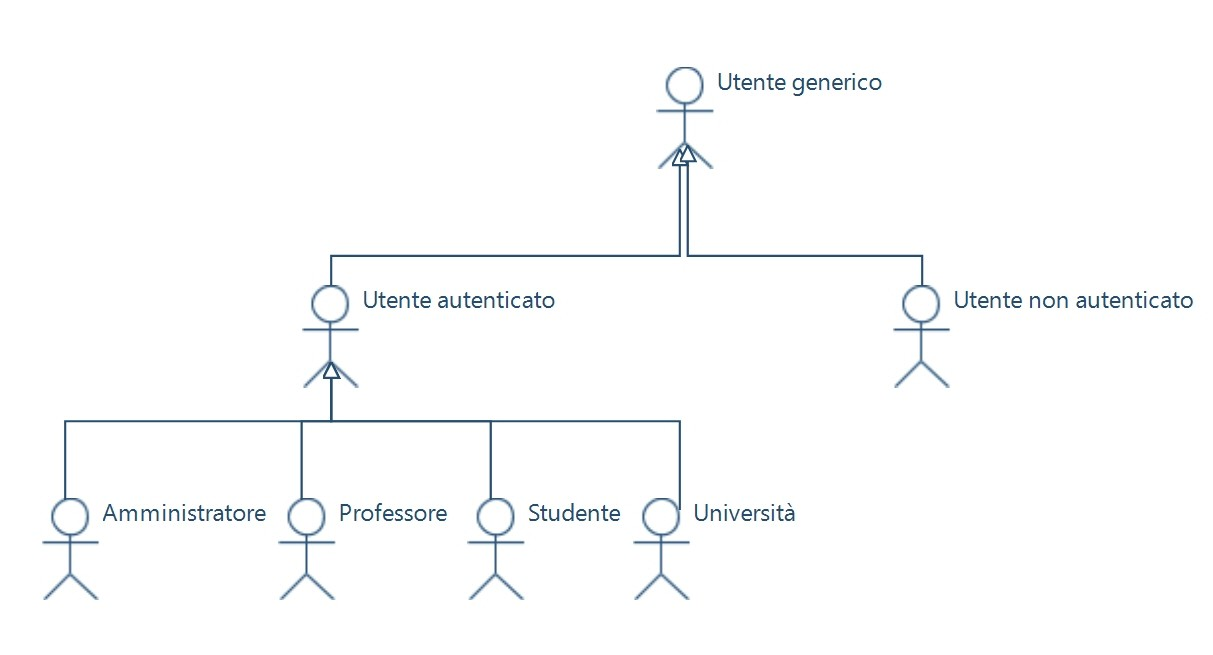
\includegraphics[width=1\linewidth]{attoriPrincipali.jpg}
		\caption{Gerarchia attori primari}
		\label{fig:Gerarchia attori primari}
	\end{figure}
	
	\item \textbf{Utente generico}\\
	Si riferisce a un utente generico che accede al sito;\\
	
	\item \textbf{Utente non autenticato}\\
	Si riferisce a un utente generico che non ha ancora effettuato il login;\\
	
	\item \textbf{Utente autenticato}\\
	 Si riferisce a un utente generico con \citGloss{indirizzo} valido e autenticato nel sistema tramite la procedura di login;\\
	
	\item \textbf{Amministratore}\\
	Si riferisce a un utente autenticato nel sistema nel ruolo di amministratore, ha i permessi per gestire i professori;\\
	
	\item \textbf{Professore}\\
	Si riferisce a un utente autenticato nel sistema nel ruolo di professore;\\
	
	\item \textbf{Studente}\\
	Si riferisce a un utente autenticato nel sistema nel ruolo di studente;\\
		
	\item \textbf{Università}\\
	Si riferisce a un utente autenticato nel sistema nel ruolo di fondatore e rappresentante dell'università, ha i permessi per gestire gli amministratori.\\	
\end{enumerate}

\subsection{Attori secondari}
\begin{enumerate}
	\item \textbf{\citGloss{MetaMask}}\\
	Plugin per \citGloss{browser} che permette di interfacciarsi a una rete \citGloss{Ethereum};\\
	
	\item \textbf{Ufficio Universitario}\\
	Entità fisica che consente l'immatricolazione degli studenti e la registrazione dei professori.\\
\end{enumerate}

\section{Elenco dei casi d'uso}
Segue un breve elenco degli scenari base per ciascun tipo di attore. Per ogni caso si può riassumere come precondizione che il sistema riconosca l'attore nel ruolo indicato dal diagramma, mentre come postcondizione che il sistema mostri le azione disponibili per il determinato attore.
Ogni scenario possibile per un attore è disponibile anche ai suoi derivati.
\begin{figure}[H]
	\centering
	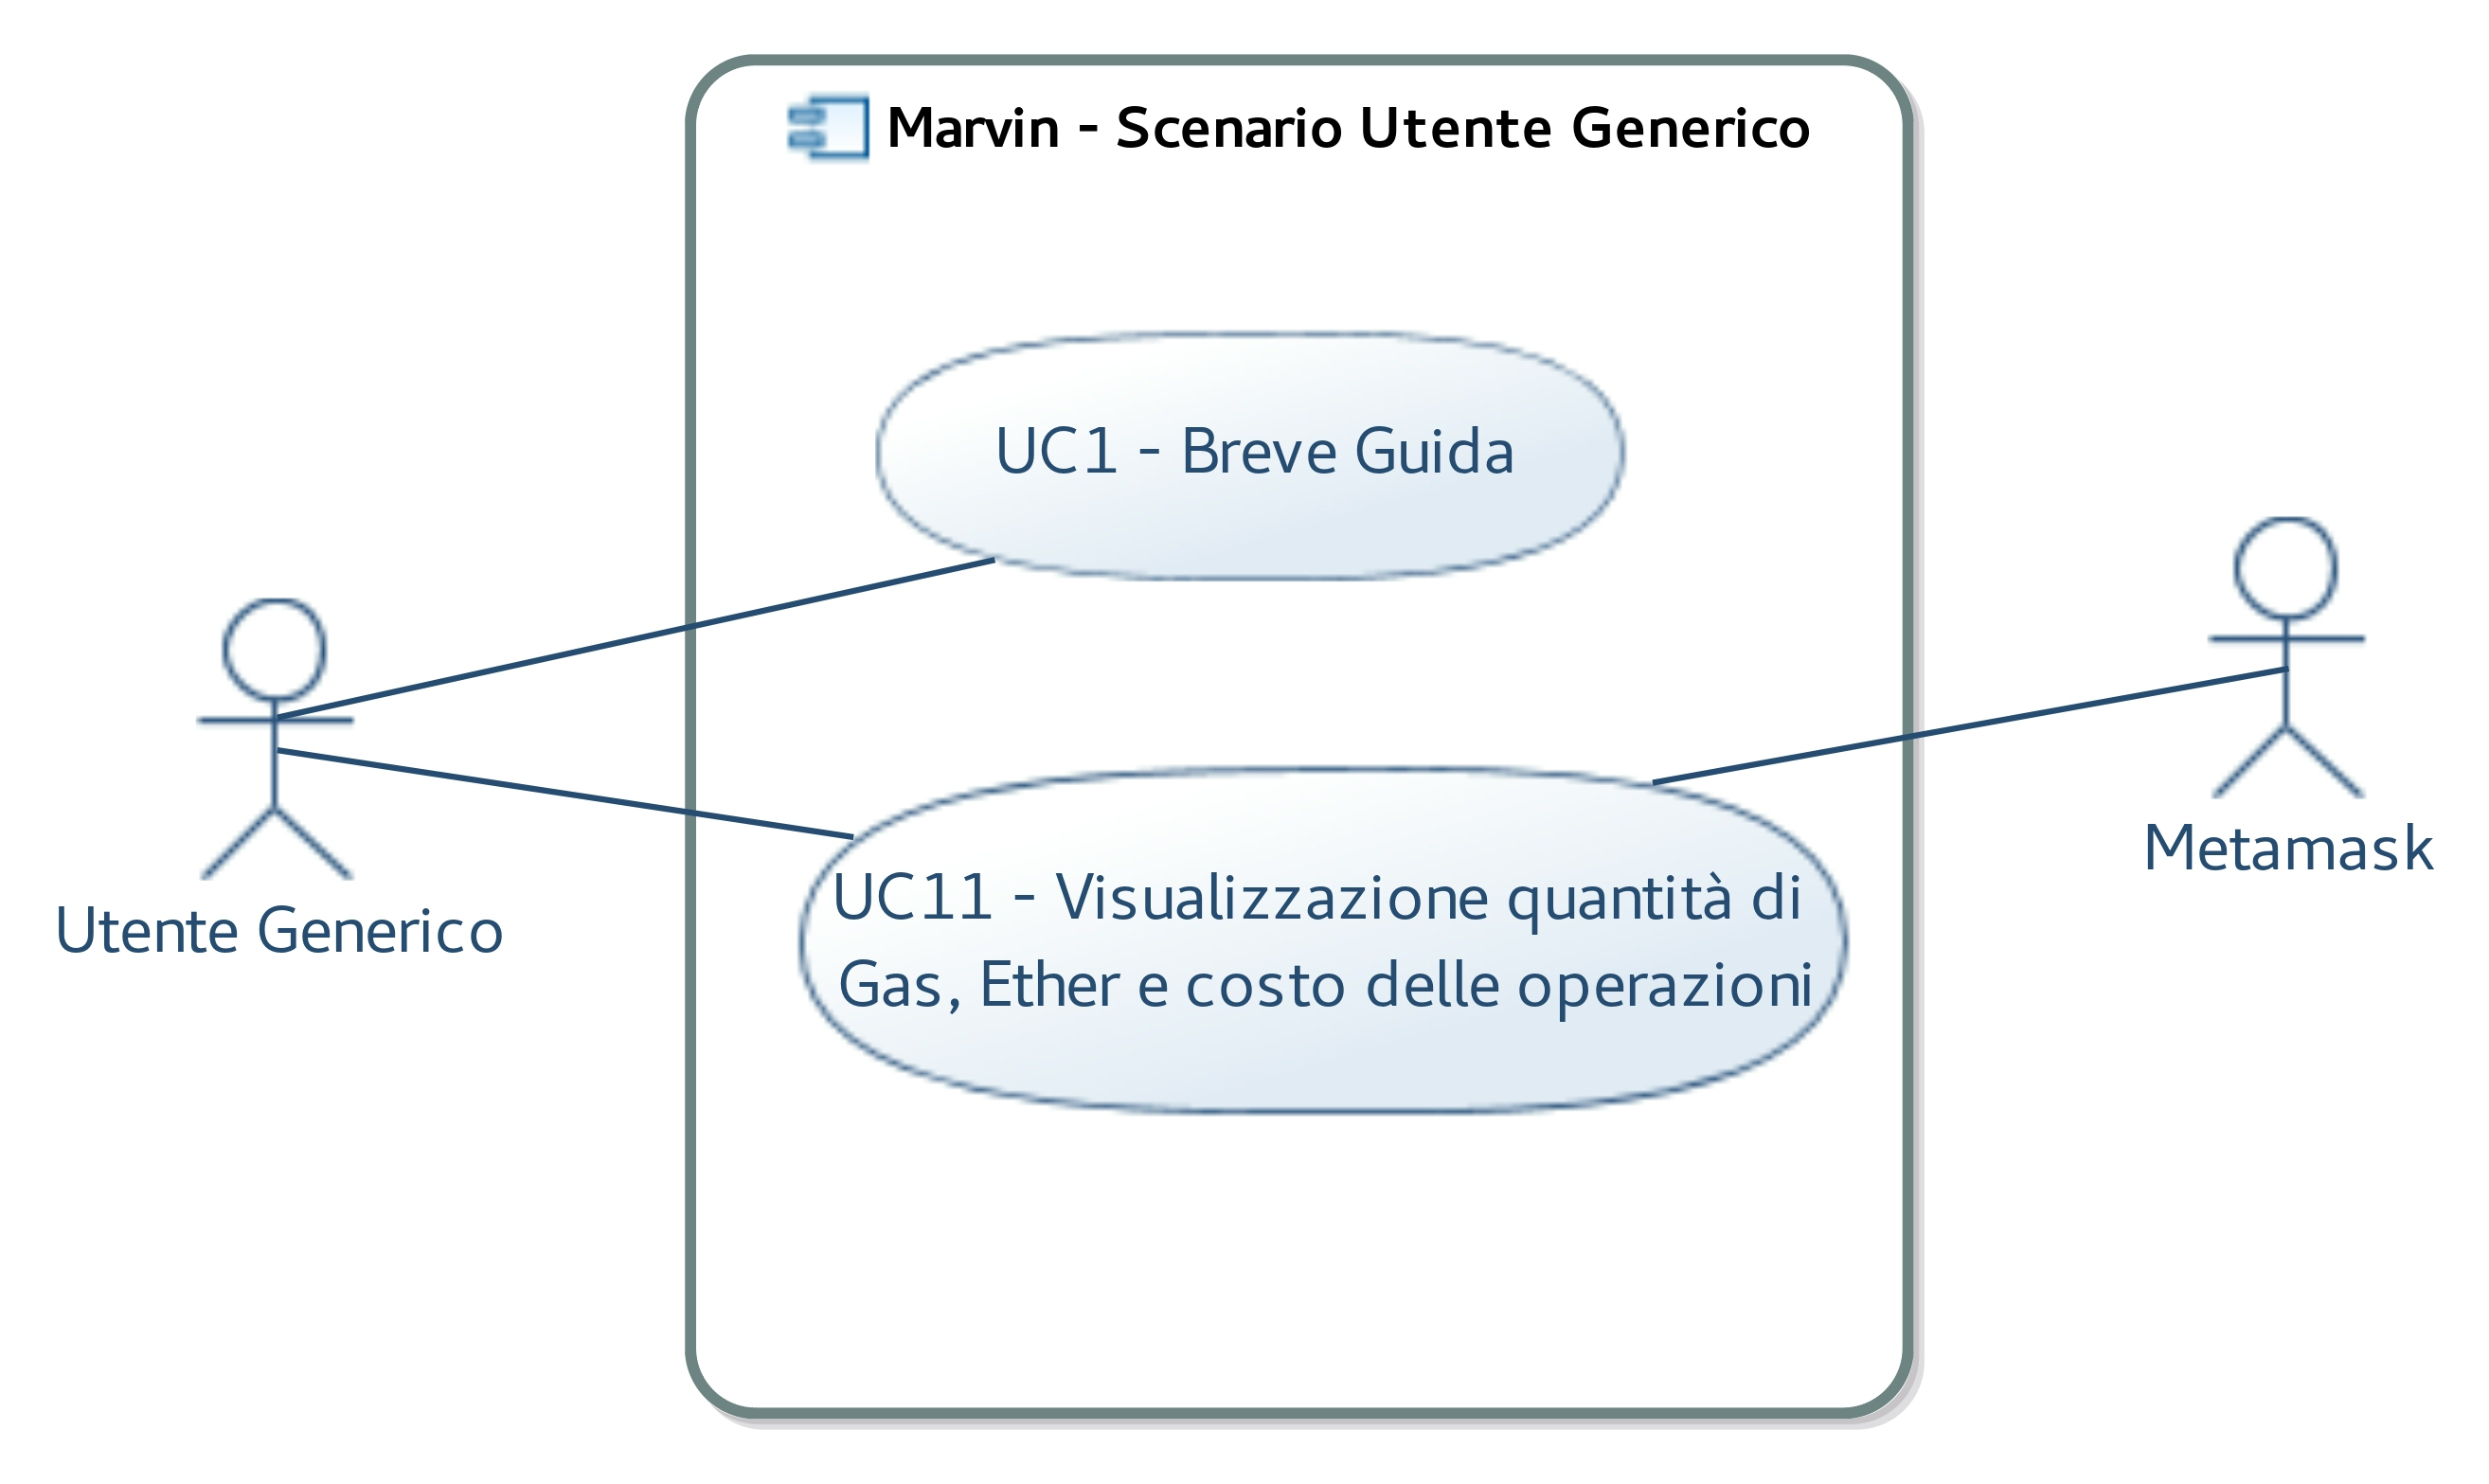
\includegraphics[width=1.0\linewidth]{UC01.jpg}
	\caption{Scenario Utente Generico}
	\label{fig:Scenario Utente Generico}
\end{figure}
\begin{figure}[H]
	\centering
	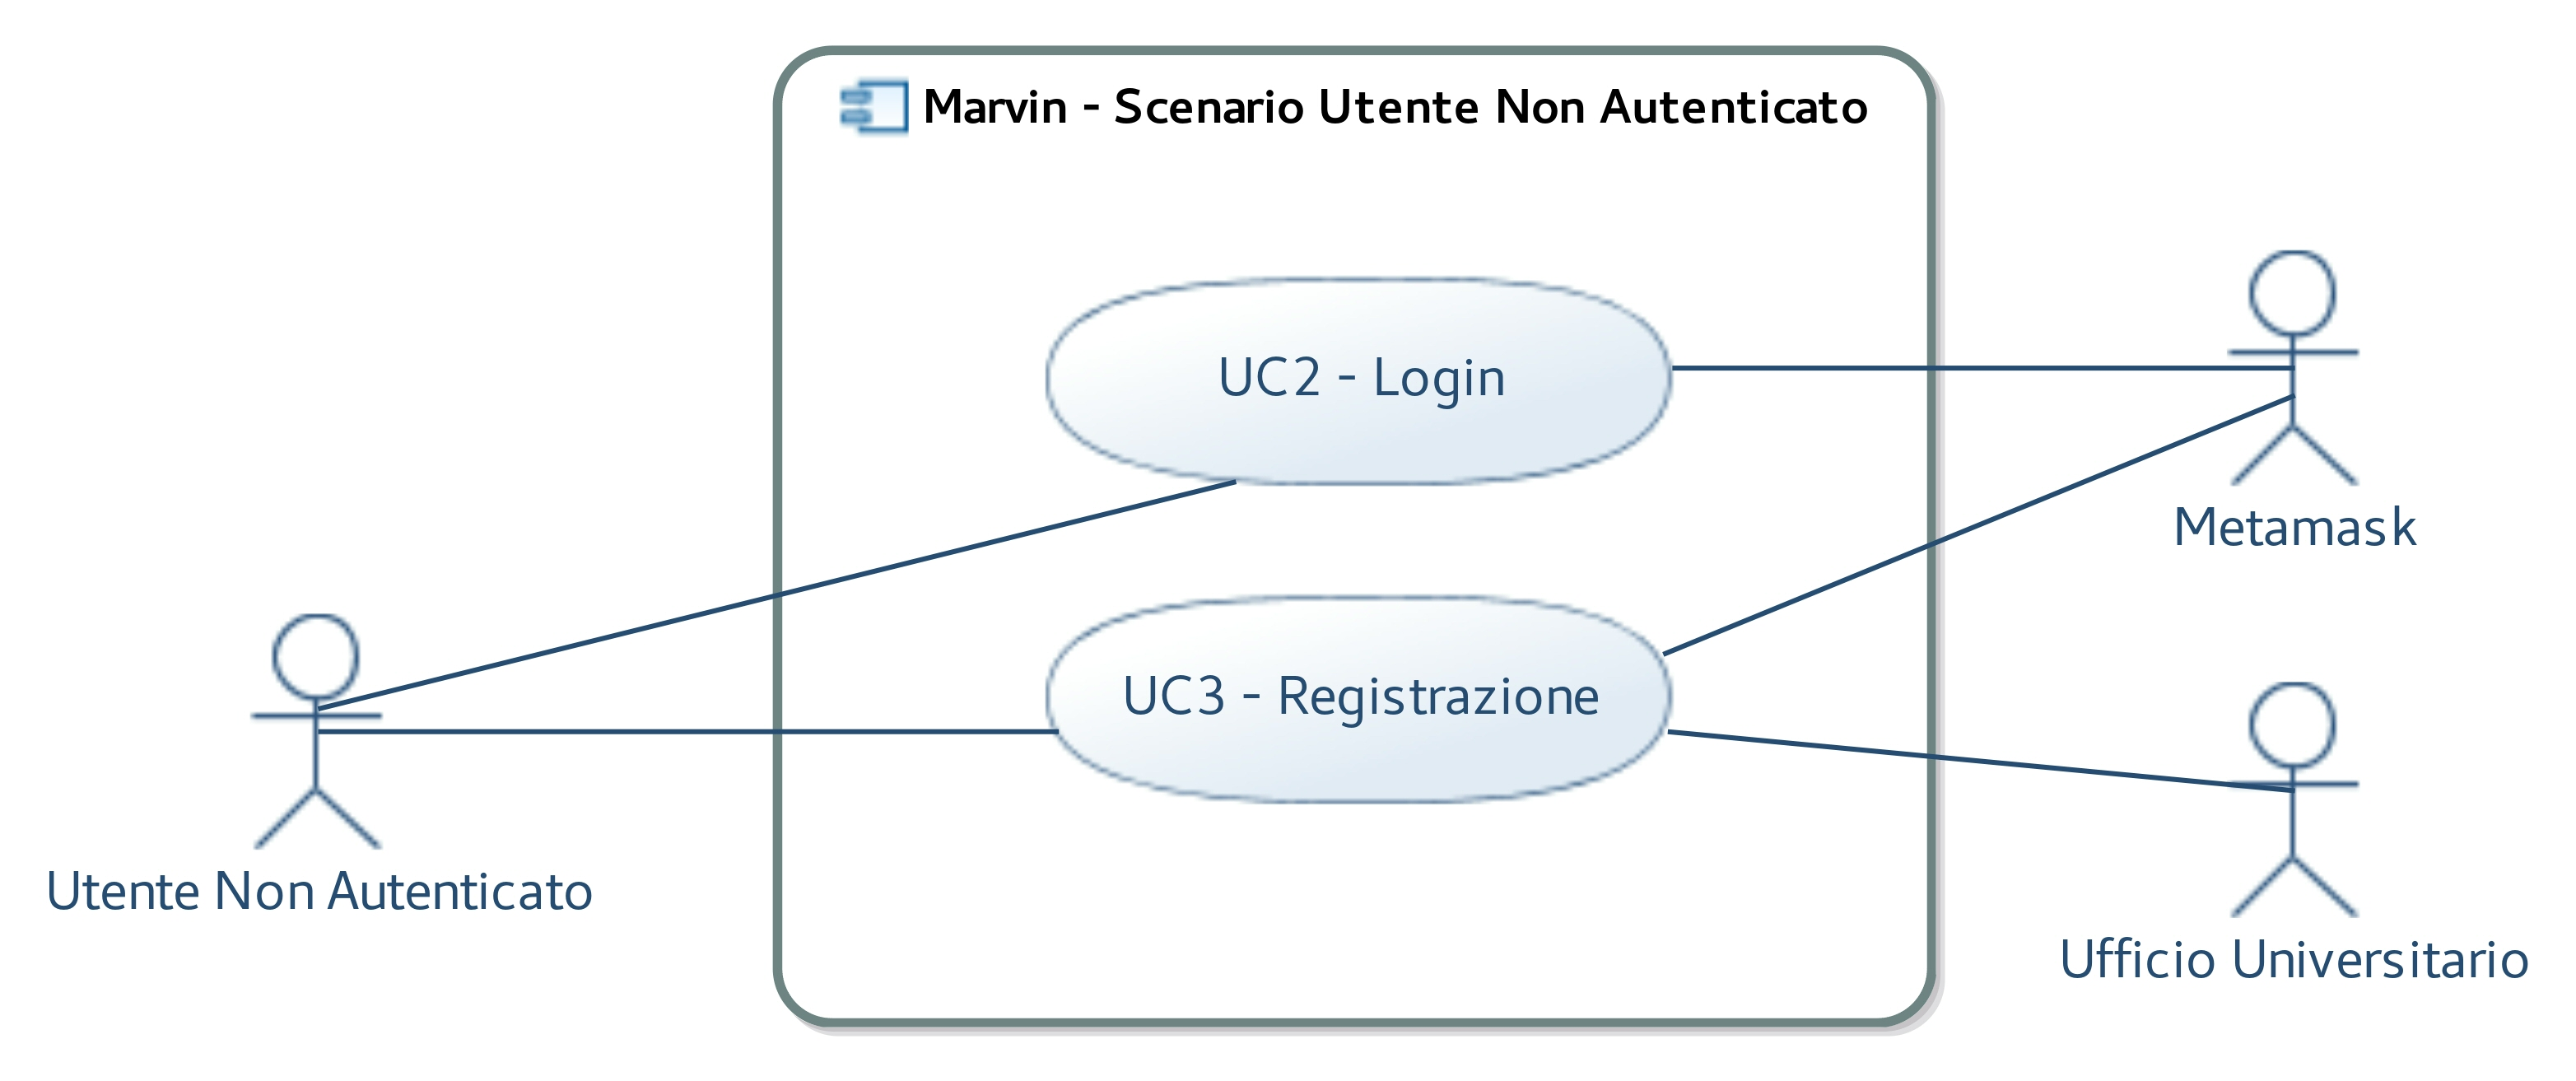
\includegraphics[width=1.0\linewidth]{UC02.jpg}
	\caption{Scenario Utente Non Autenticato}
	\label{fig:Scenario Utente Non Autenticato}
\end{figure}
\begin{figure}[H]
	\centering
	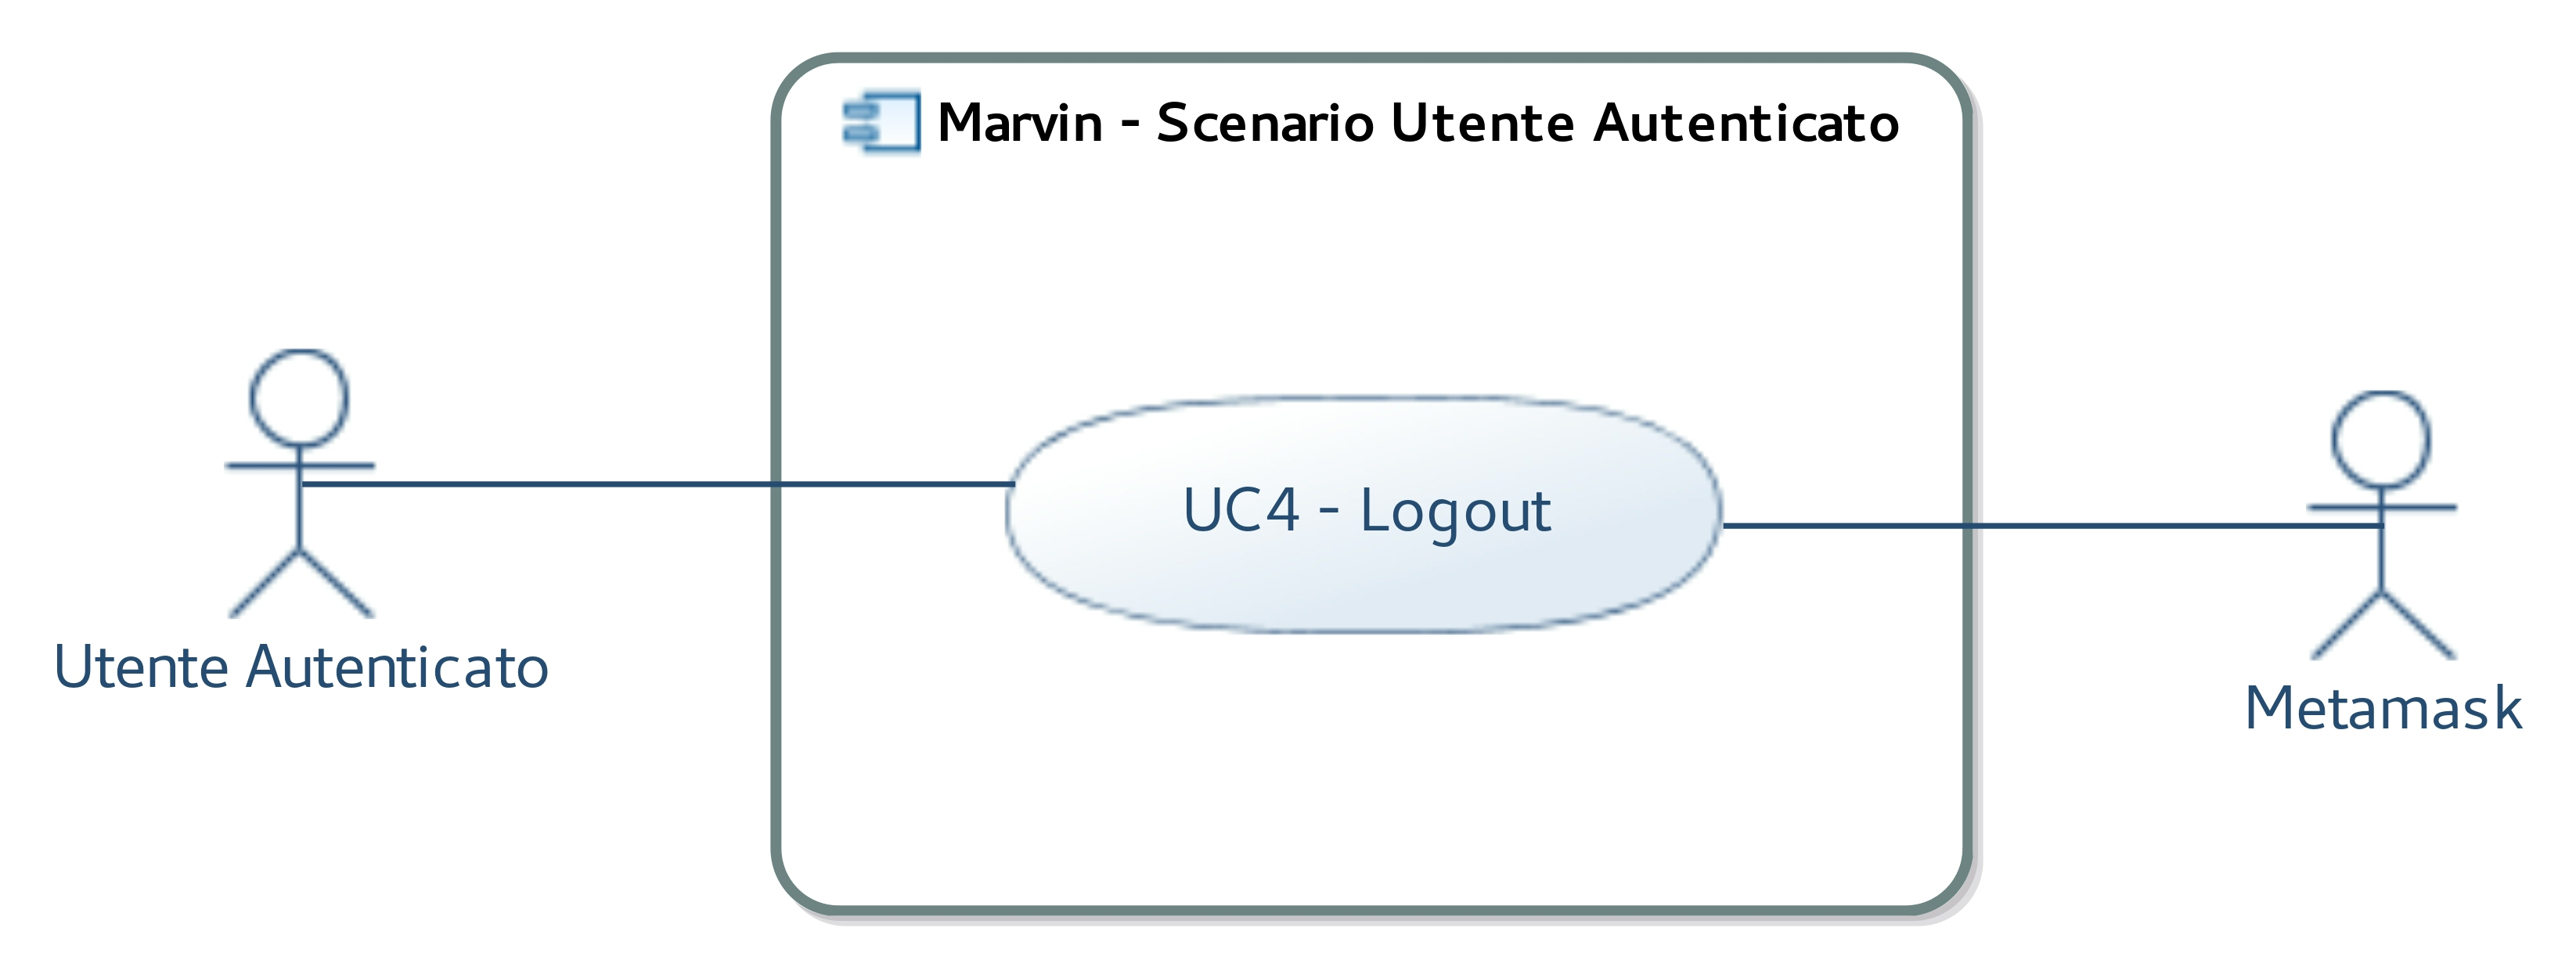
\includegraphics[width=1.0\linewidth]{UC03.jpg}
	\caption{Scenario Utente Autenticato}
	\label{fig:Scenario Utente Autenticato}
\end{figure}
\begin{figure}[H]
	\centering
	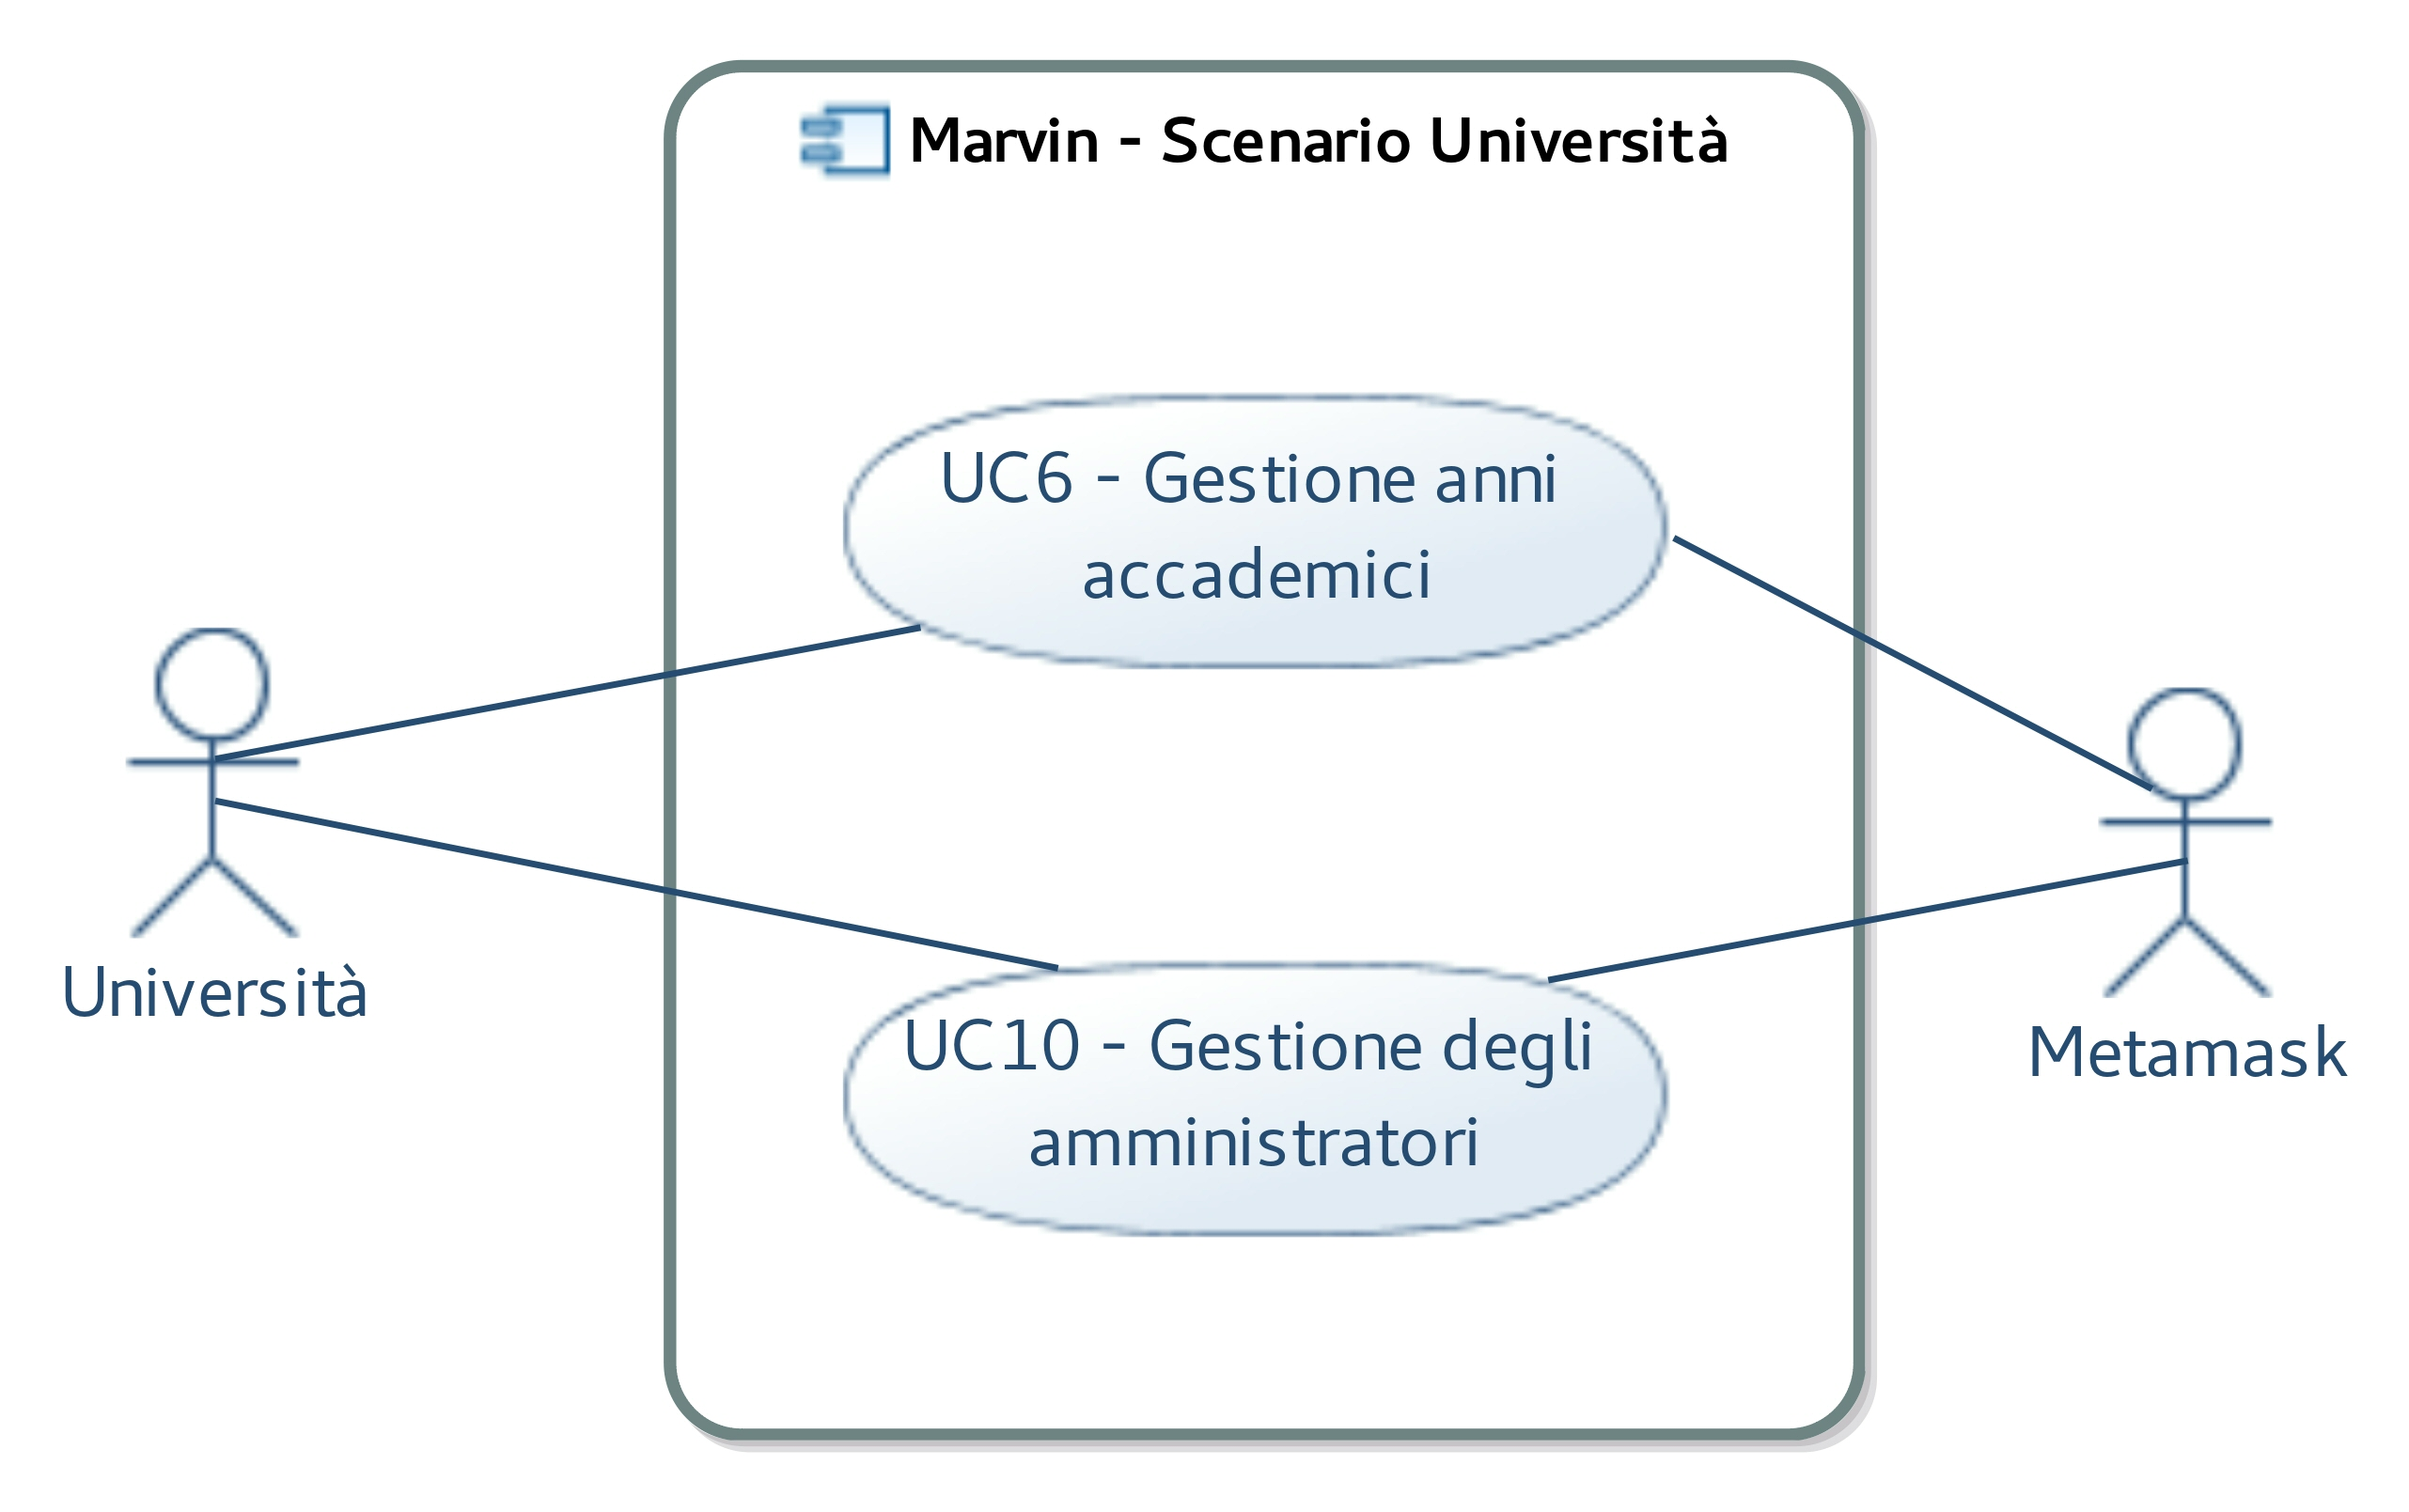
\includegraphics[width=1.0\linewidth]{UC07.jpg}
	\caption{Scenario Universita}
	\label{fig:Scenario Universita}
\end{figure}
\begin{figure}[H]
	\centering
	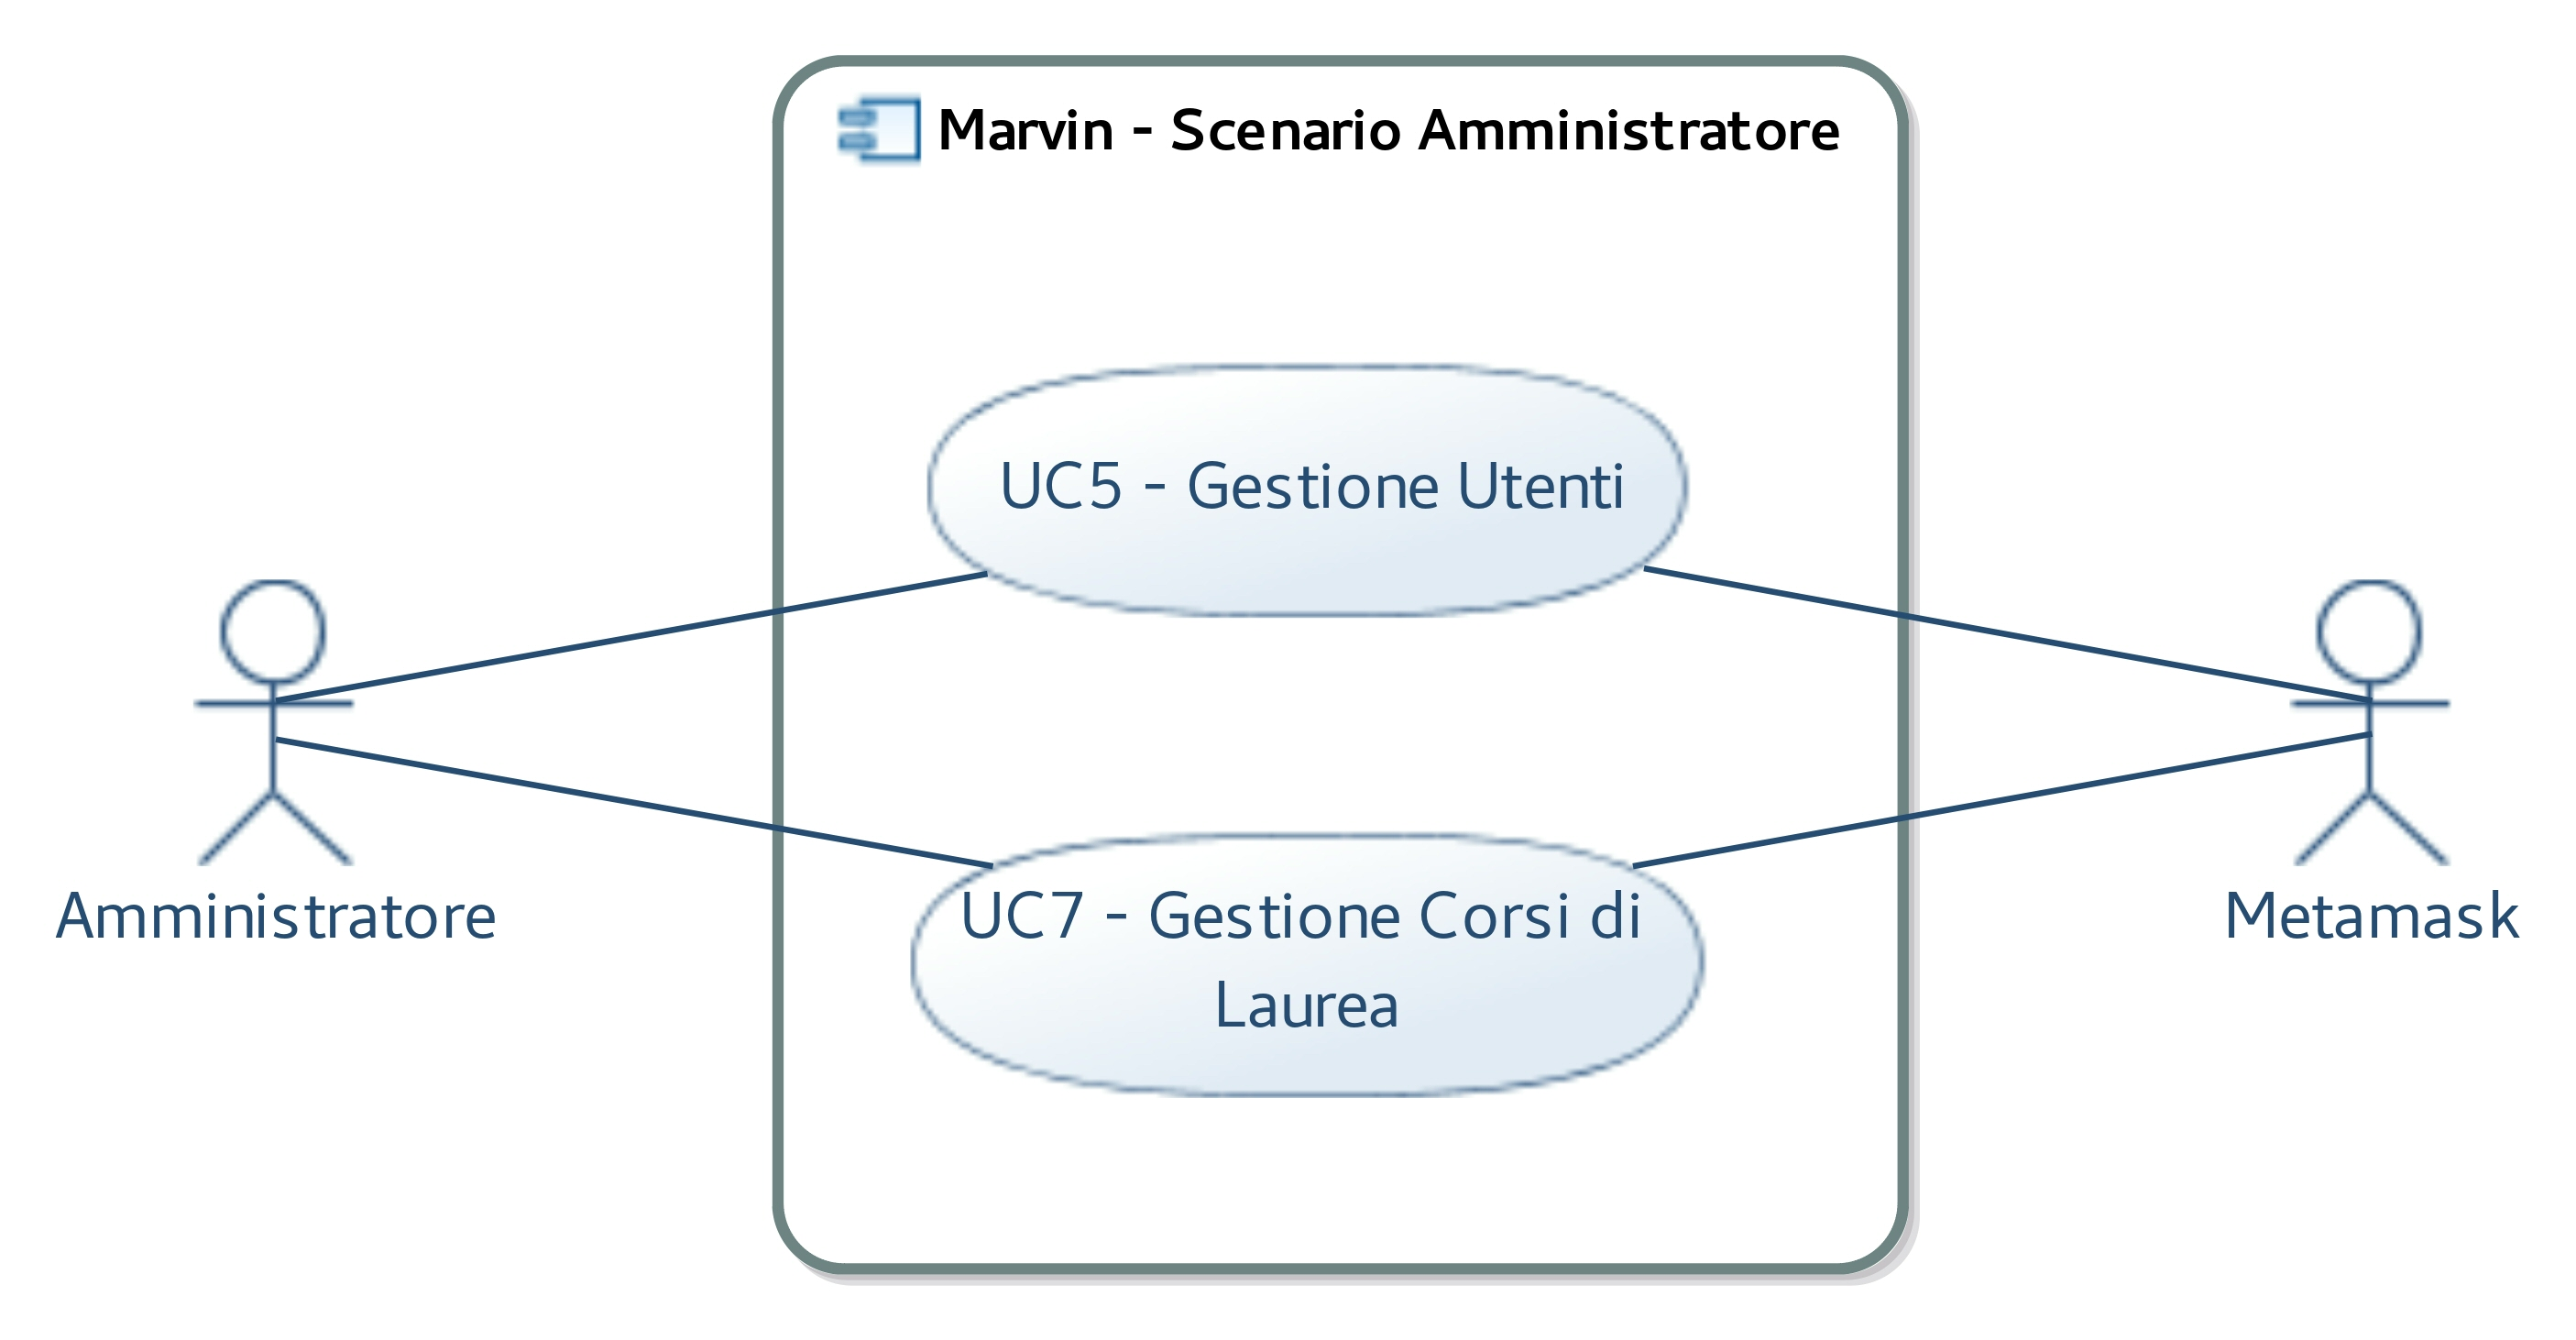
\includegraphics[width=1.0\linewidth]{UC04.jpg}
	\caption{Scenario Amministratore}
	\label{fig:Scenario Amministratore}
\end{figure}
\begin{figure}[H]
	\centering
	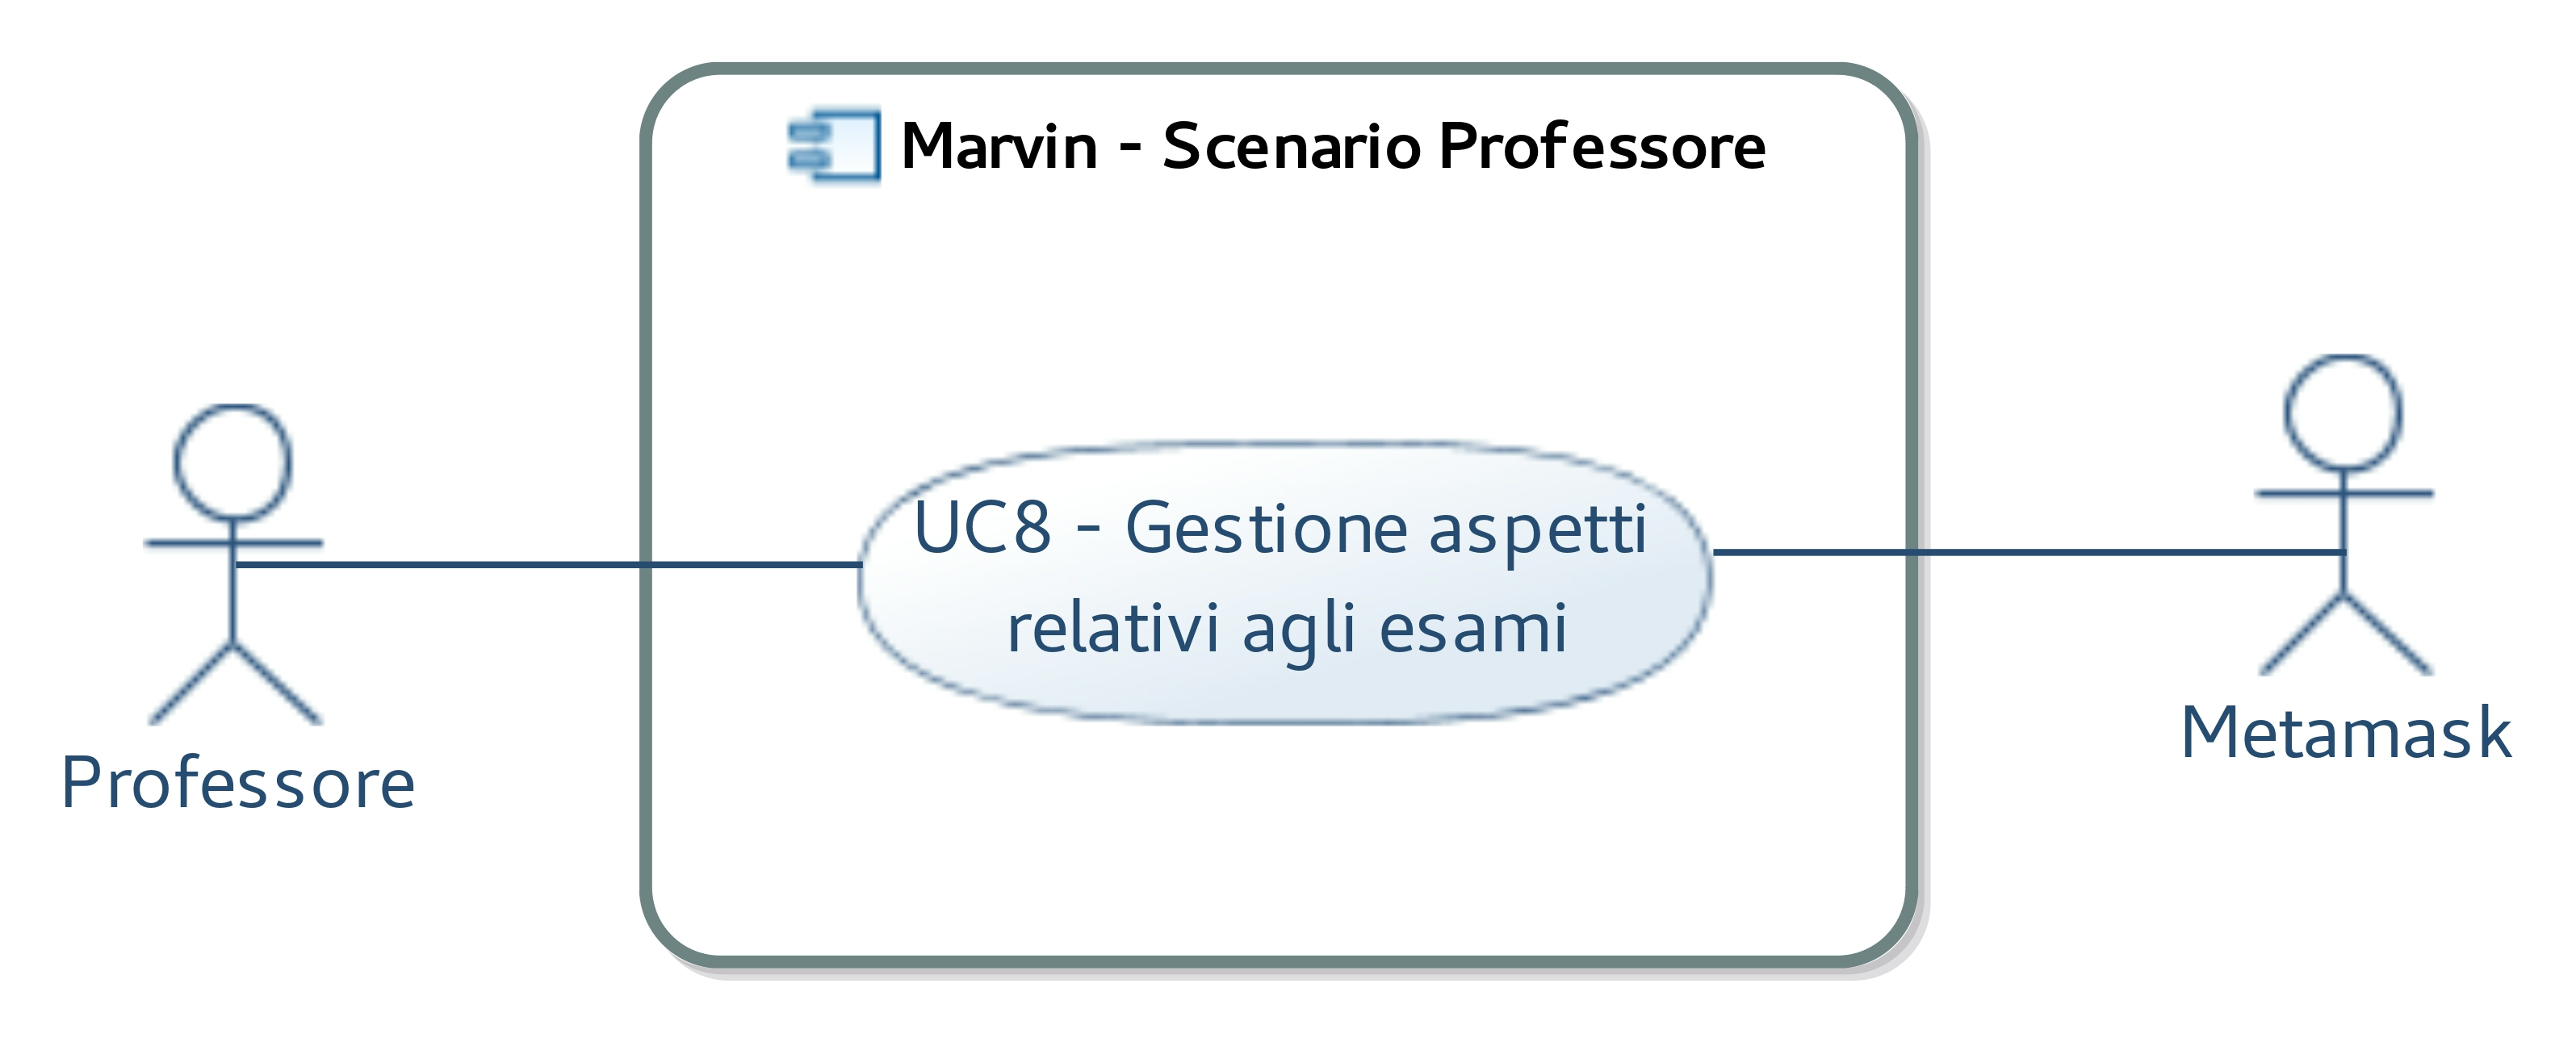
\includegraphics[width=1.0\linewidth]{UC05.jpg}
	\caption{Scenario Professore}
	\label{fig:Scenario Professore}
\end{figure}
\begin{figure}[H]
	\centering
	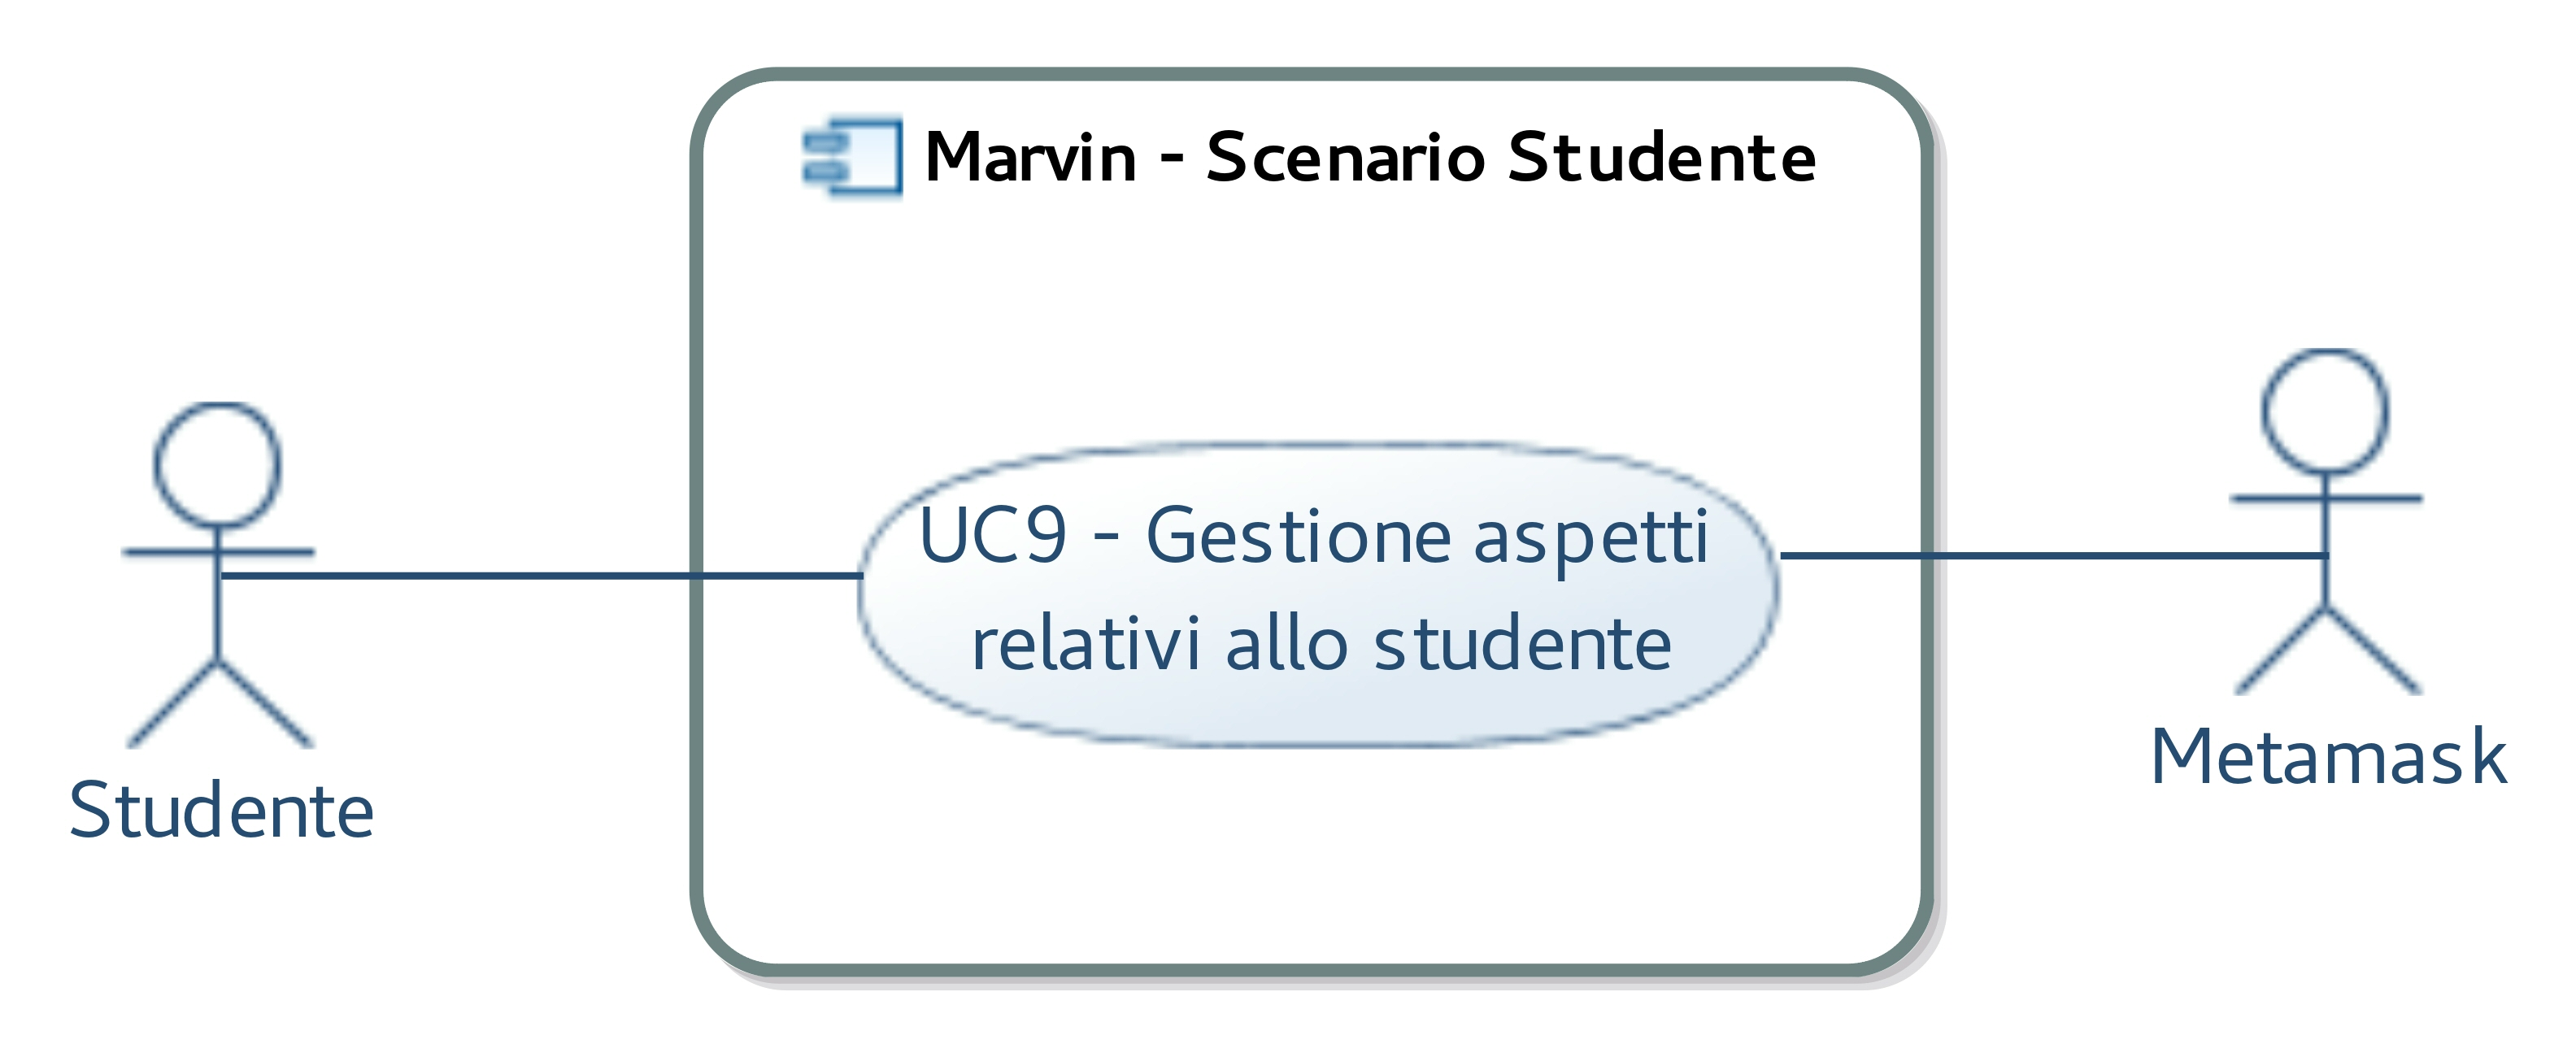
\includegraphics[width=1.0\linewidth]{UC06.jpg}
	\caption{Scenario Studente}
	\label{fig:Scenario Studente}
\end{figure}


%   -------------------------------------------------------------------------------------
%   ----------                 MODELLO PER GLI USER CASE              -------------------
%   -------------------------------------------------------------------------------------
\begin{comment}
\subsection{UCX - Nome}
\begin{itemize}
	\item \textbf{Attori primari:} ;\\
	\item \textbf{Attori secondari:} ;\\
	\item \textbf{Scopo e descrizione:} ;\\
	\item \textbf{Scenario principale:} ;\\
	\item \textbf{Scenario alternativo:} ;\\
	\item \textbf{Flusso principale degli eventi:};\\
	\begin{enumerate}
		\item L'utente... ;
		\item L'utente... ;
	\end{enumerate}
	\item \textbf{Estensioni:}\\
		\begin{enumerate}
		\item Se l'utente... ;[UCX.X.X]
	\end{enumerate}
	\item \textbf{Precondizione:} ;\\
	\item \textbf{Postcondizione:} .\\
\end{itemize}
\end{comment}

\subsection{UC1 - Breve guida}
\begin{itemize}
	\item \textbf{Attori primari:} utente generico;
	\item \textbf{Scopo e descrizione:} l'utente visualizza una breve guida di introduzione su come installare il plugin \citGloss{MetaMask} e su come gestire le chiavi in modo da istruirlo sulle modalità di accesso al sistema;
	\item \textbf{Scenario principale:} l'utente accede alla guida;
	\item \textbf{Precondizione:} il sistema è raggiungibile e funzionante e l'utente desidera aprire la guida;
	\item \textbf{Postcondizione:} il sistema fornisce la guida e l'utente riceve delle nozioni riguardanti l'accesso al sistema.
\end{itemize}
\subsection{UC2 - Login}
\begin{itemize}
	\item \textbf{Attori primari:} utente non autenticato;
	\item \textbf{Attori secondari:} \citGloss{MetaMask};
	\item \textbf{Scopo e descrizione:} l'utente richiede il login al sistema attraverso il plugin \citGloss{MetaMask};
	\item \textbf{Scenario principale:} l'utente non ancora riconosciuto dal sistema effettua il login;
	\item \textbf{Precondizione:} il sistema considera l'utilizzatore come un utente non autenticato;
	\item \textbf{Postcondizione:} il sistema riconosce l'utilizzatore come un utente autenticato.\\
\end{itemize}

\begin{figure}[H]
	\centering
	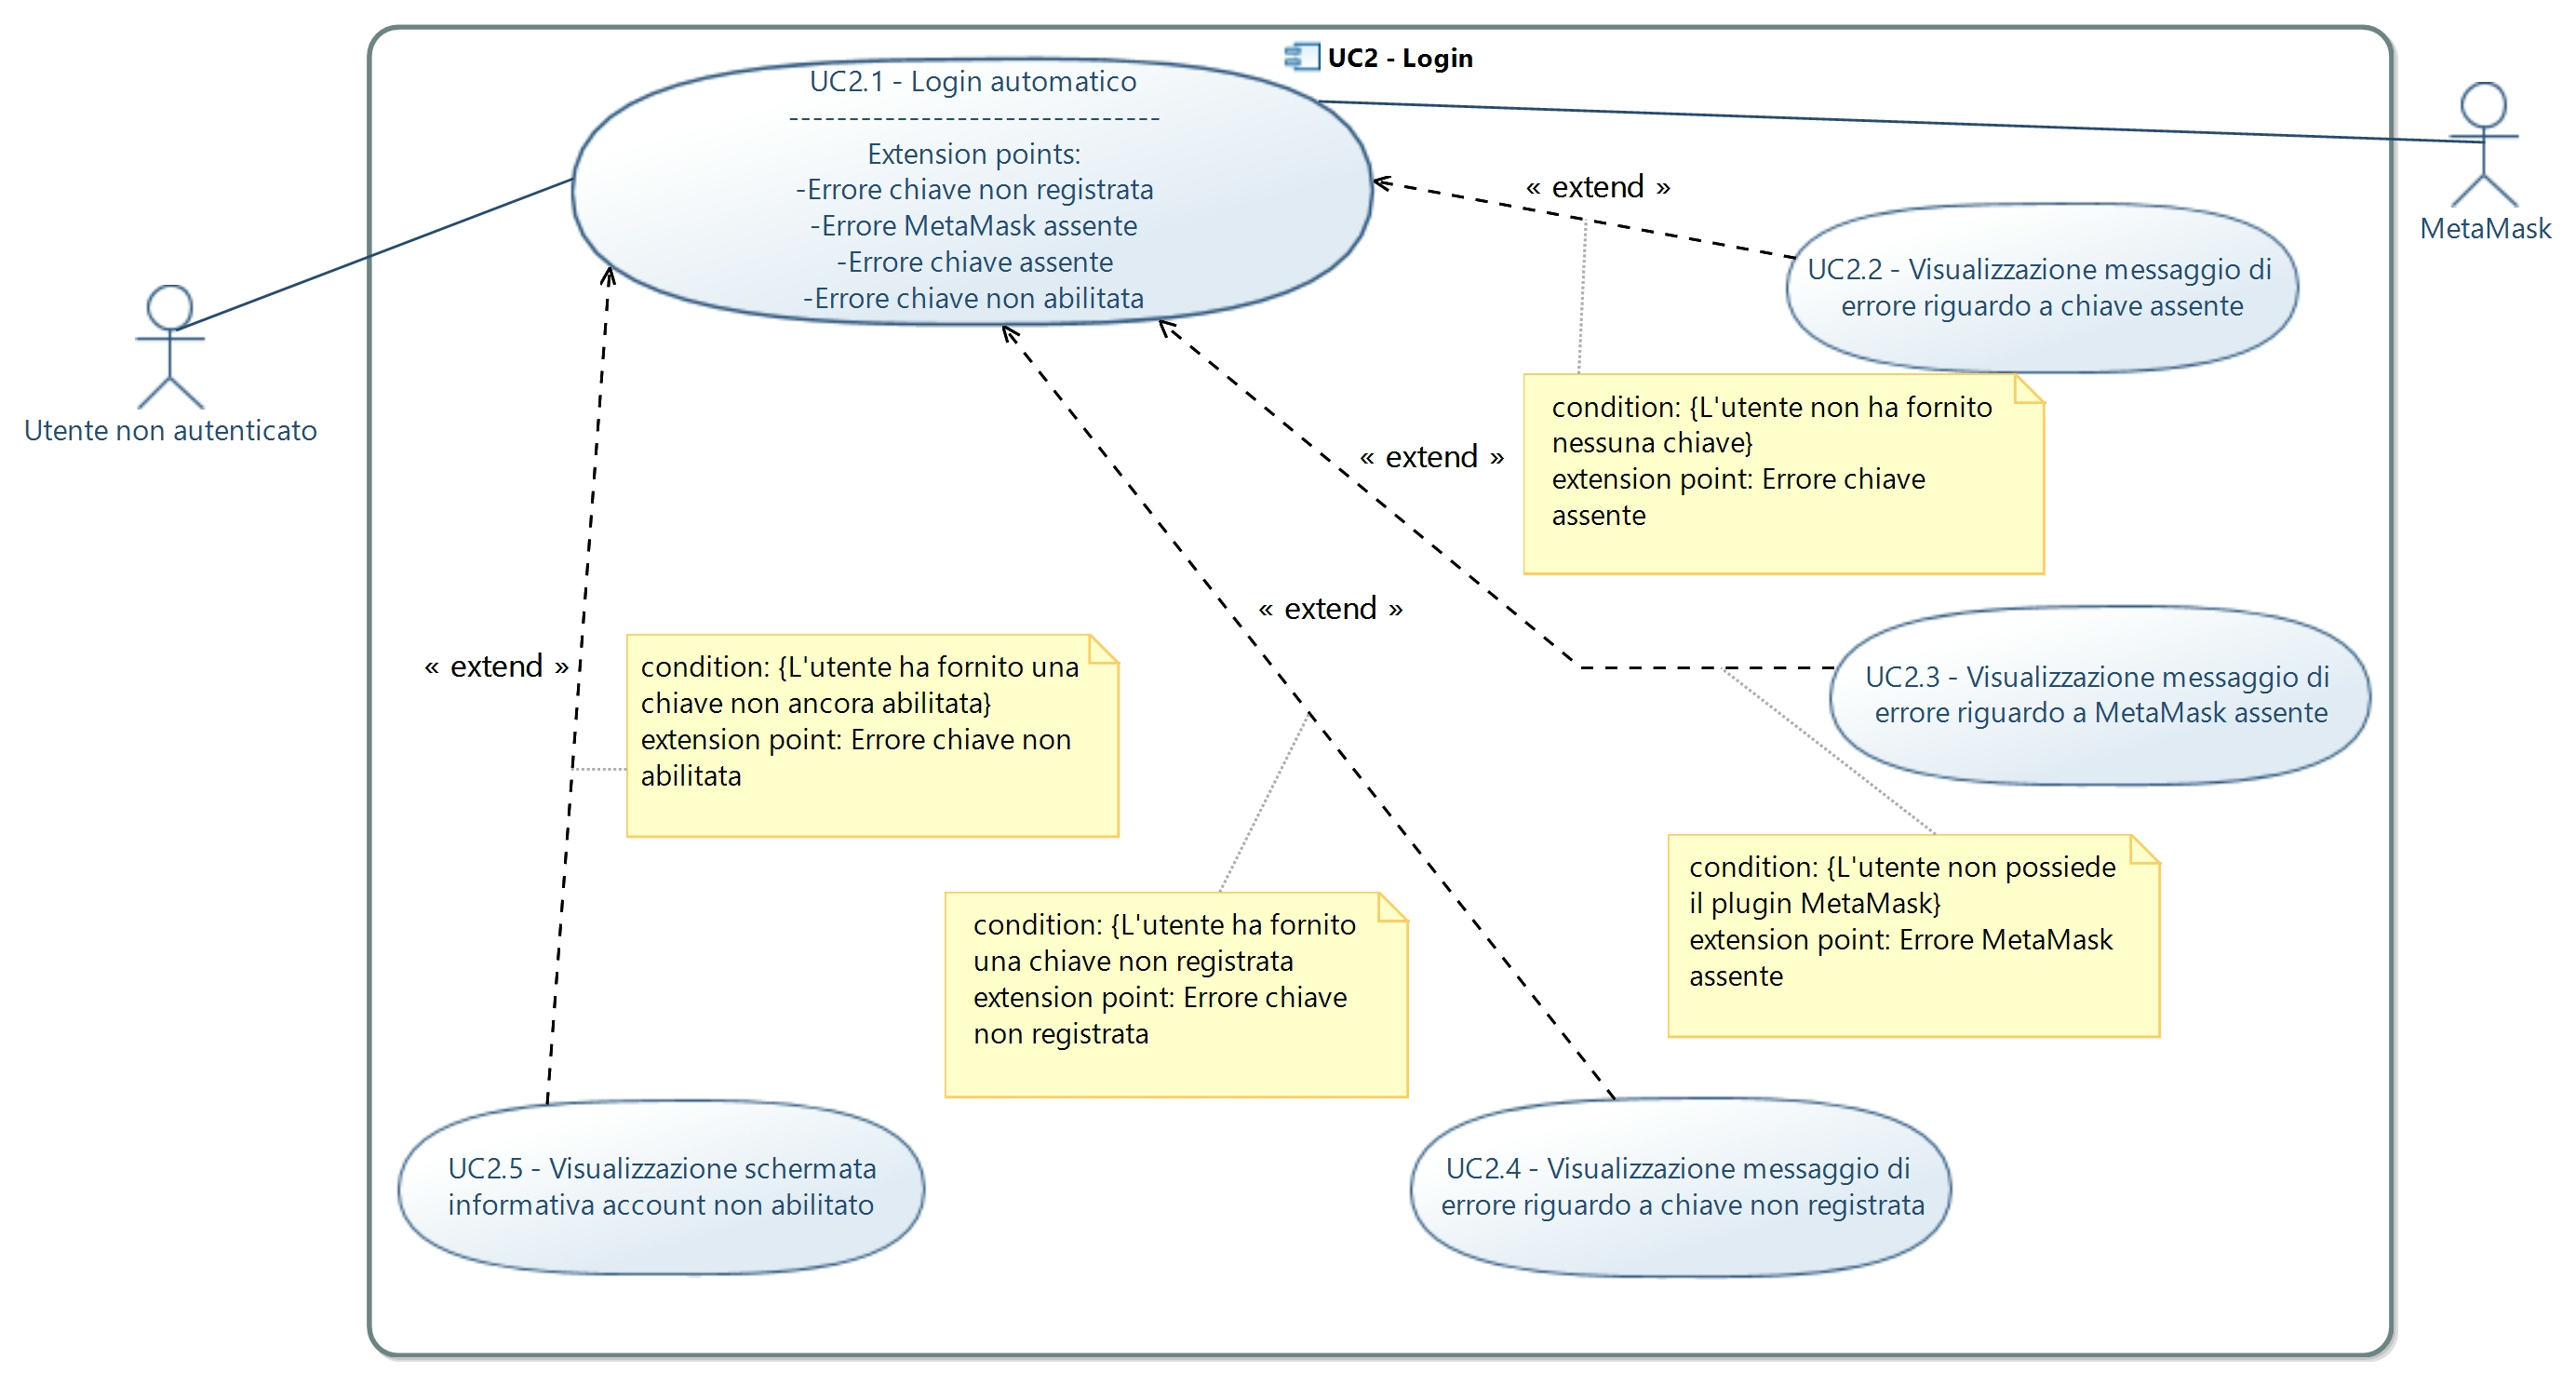
\includegraphics[width=1.0\linewidth]{UC2.jpg}
	\caption{UC2 - Login}
	\label{fig:UC2 - Login}
\end{figure}

\subsection{UC2.1 - Login automatico}
\begin{itemize}
\item \textbf{Attori primari:} utente non autenticato;
\item \textbf{Attori secondari:} \citGloss{MetaMask};
\item \textbf{Scopo e descrizione:} l'utente attende il login da parte del sistema senza effettuare nessuna operazione aggiuntiva;
\item \textbf{Scenario principale:} l'utente non ancora riconosciuto dal sistema richiede il login;
\item \textbf{Estensioni:}
\begin{enumerate}
	\item Se l'utente non ha a disposizione una \citGloss{chiave} viene avvisato con un errore a riguardo [UC2.2];
	\item Se l'utente non ha il plugin \citGloss{MetaMask} installato nel \citGloss{browser} viene avvisato con un errore a riguardo [UC2.3];
	\item Se l'utente ha a disposizione una \citGloss{chiave} non registrata viene avvisato con un errore a riguardo [UC2.4];
	\item Se l'utente tenta di fare il login con un account in attesa di approvazione viene avvisato con una schermata informativa a riguardo [UC2.5].
\end{enumerate}
\item \textbf{Precondizione:} il sistema considera l'utilizzatore come un utente non autenticato;
\item \textbf{Postcondizione:} il sistema, grazie a una interazione con \citGloss{MetaMask}, riconosce l'utente come autenticato.
\end{itemize}
\subsection{UC2.2 - Visualizzazione messaggio di errore riguardo a \citGloss{chiave} assente}
\begin{itemize}
	\item \textbf{Attori primari:} utente non autenticato;
	\item \textbf{Scopo e descrizione:} l'utente viene avvisato del fatto che non è stato possibile da parte del sistema il recupero della \citGloss{chiave};
	\item \textbf{Scenario principale:} l'utente visualizza l'errore relativo all'assenza di una \citGloss{chiave} per accedere al sistema;
	\item \textbf{Precondizione:} il sistema riceve una richiesta di login da parte di un utente non in possesso di una \citGloss{chiave};
	\item \textbf{Postcondizione:} il sistema avvisa l'utente di dover interagire con \citGloss{MetaMask} per poter fornire una \citGloss{chiave}.
\end{itemize}
\subsection{UC2.3 - Visualizzazione messaggio di errore riguardo a \citGloss{MetaMask} assente}
\begin{itemize}
	\item \textbf{Attori primari:} utente non autenticato;
	\item \textbf{Scopo e descrizione:} l'utente viene avvisato del fatto sta cercando di accedere al sistema senza il plugin \citGloss{MetaMask};
	\item \textbf{Scenario principale:} l'utente visualizza il messaggio d'errore relativo alla mancanza del plugin \citGloss{MetaMask};
	\item \textbf{Precondizione:} il sistema riceve una richiesta di login da parte di un utente che non ha installato nel browser attualmente in uso il plugin \citGloss{MetaMask};
	\item \textbf{Postcondizione:} il sistema avvisa l'utente della necessità di possedere \citGloss{MetaMask} per poter accedere.
\end{itemize}
\subsection{UC2.4 - Visualizzazione messaggio di errore riguardo a chiave non registrata}
\begin{itemize}
	\item \textbf{Attori primari:} utente non autenticato;
	\item \textbf{Scopo e descrizione:} l'utente viene avvisato del fatto che ha fornito una \citGloss{chiave} non registrata nel sistema;
	\item \textbf{Scenario principale:} l'utente viene informato che la sua \citGloss{chiave} non risulta registrata, in quanto il relativo \citGloss{indirizzo} non è presente nel sistema, suggerendone la registrazione;
	\item \textbf{Precondizione:} il sistema riceve una richiesta di login da parte di un utente che sta utilizzando una \citGloss{chiave} non registrata;
	\item \textbf{Postcondizione:} il sistema avvisa l'utente della necessità di dover effettuare la registrazione per accedere al sistema.
\end{itemize}
\subsection{UC2.5 - Visualizzazione schermata informativa account non abilitato}
\begin{itemize}
	\item \textbf{Attori primari:} utente non autenticato;
	\item \textbf{Scopo e descrizione:} l'utente viene informato che il suo \citGloss{indirizzo} non è ancora stato abilitato all'uso dei servizi;
	\item \textbf{Scenario principale:} il sistema mostra una schermata informativa per avvisare l'utente che il suo account è in attesa di essere abilitato;
	\item \textbf{Precondizione:} il sistema riceve una richiesta di login da parte di un utente senza che il suo account sia stato precedentemente abilitato da un amministratore;
	\item \textbf{Postcondizione:} il sistema avvisa l'utente della necessità di dover attendere l'abilitazione del suo account da parte di un amministratore per accedere al sistema.
\end{itemize}
\subsection{UC3 - Registrazione}
\begin{itemize}
	\item \textbf{Attori primari:} utente non autenticato;
	\item \textbf{Attori secondari:} \citGloss{MetaMask}, Ufficio Universitario;
	\item \textbf{Scopo e descrizione:} l'utente non autenticato compila i campi richiesti per registrarsi nel sistema, successivamente si dovrà presentare all'ufficio universitario con i documenti per l'identificazione;
	\item \textbf{Scenario principale:}
	\begin{enumerate}
		\item L'utente inserisce il suo nome [UC3.1];
		\item L'utente inserisce il suo cognome [UC3.2];
		\item L'utente seleziona la sua categoria [UC3.3];
		\item L'utente seleziona il corso desiderato [UC3.4].
	\end{enumerate}
	\item \textbf{Precondizione:} il sistema considera l'utilizzatore come un utente non autenticato, il quale desidera procedere con la registrazione;
	\item \textbf{Postcondizione:} il sistema riceve la richiesta di registrazione, registrando le informazioni immesse dall'utente.
\end{itemize}

\begin{figure}[H]
	\centering
	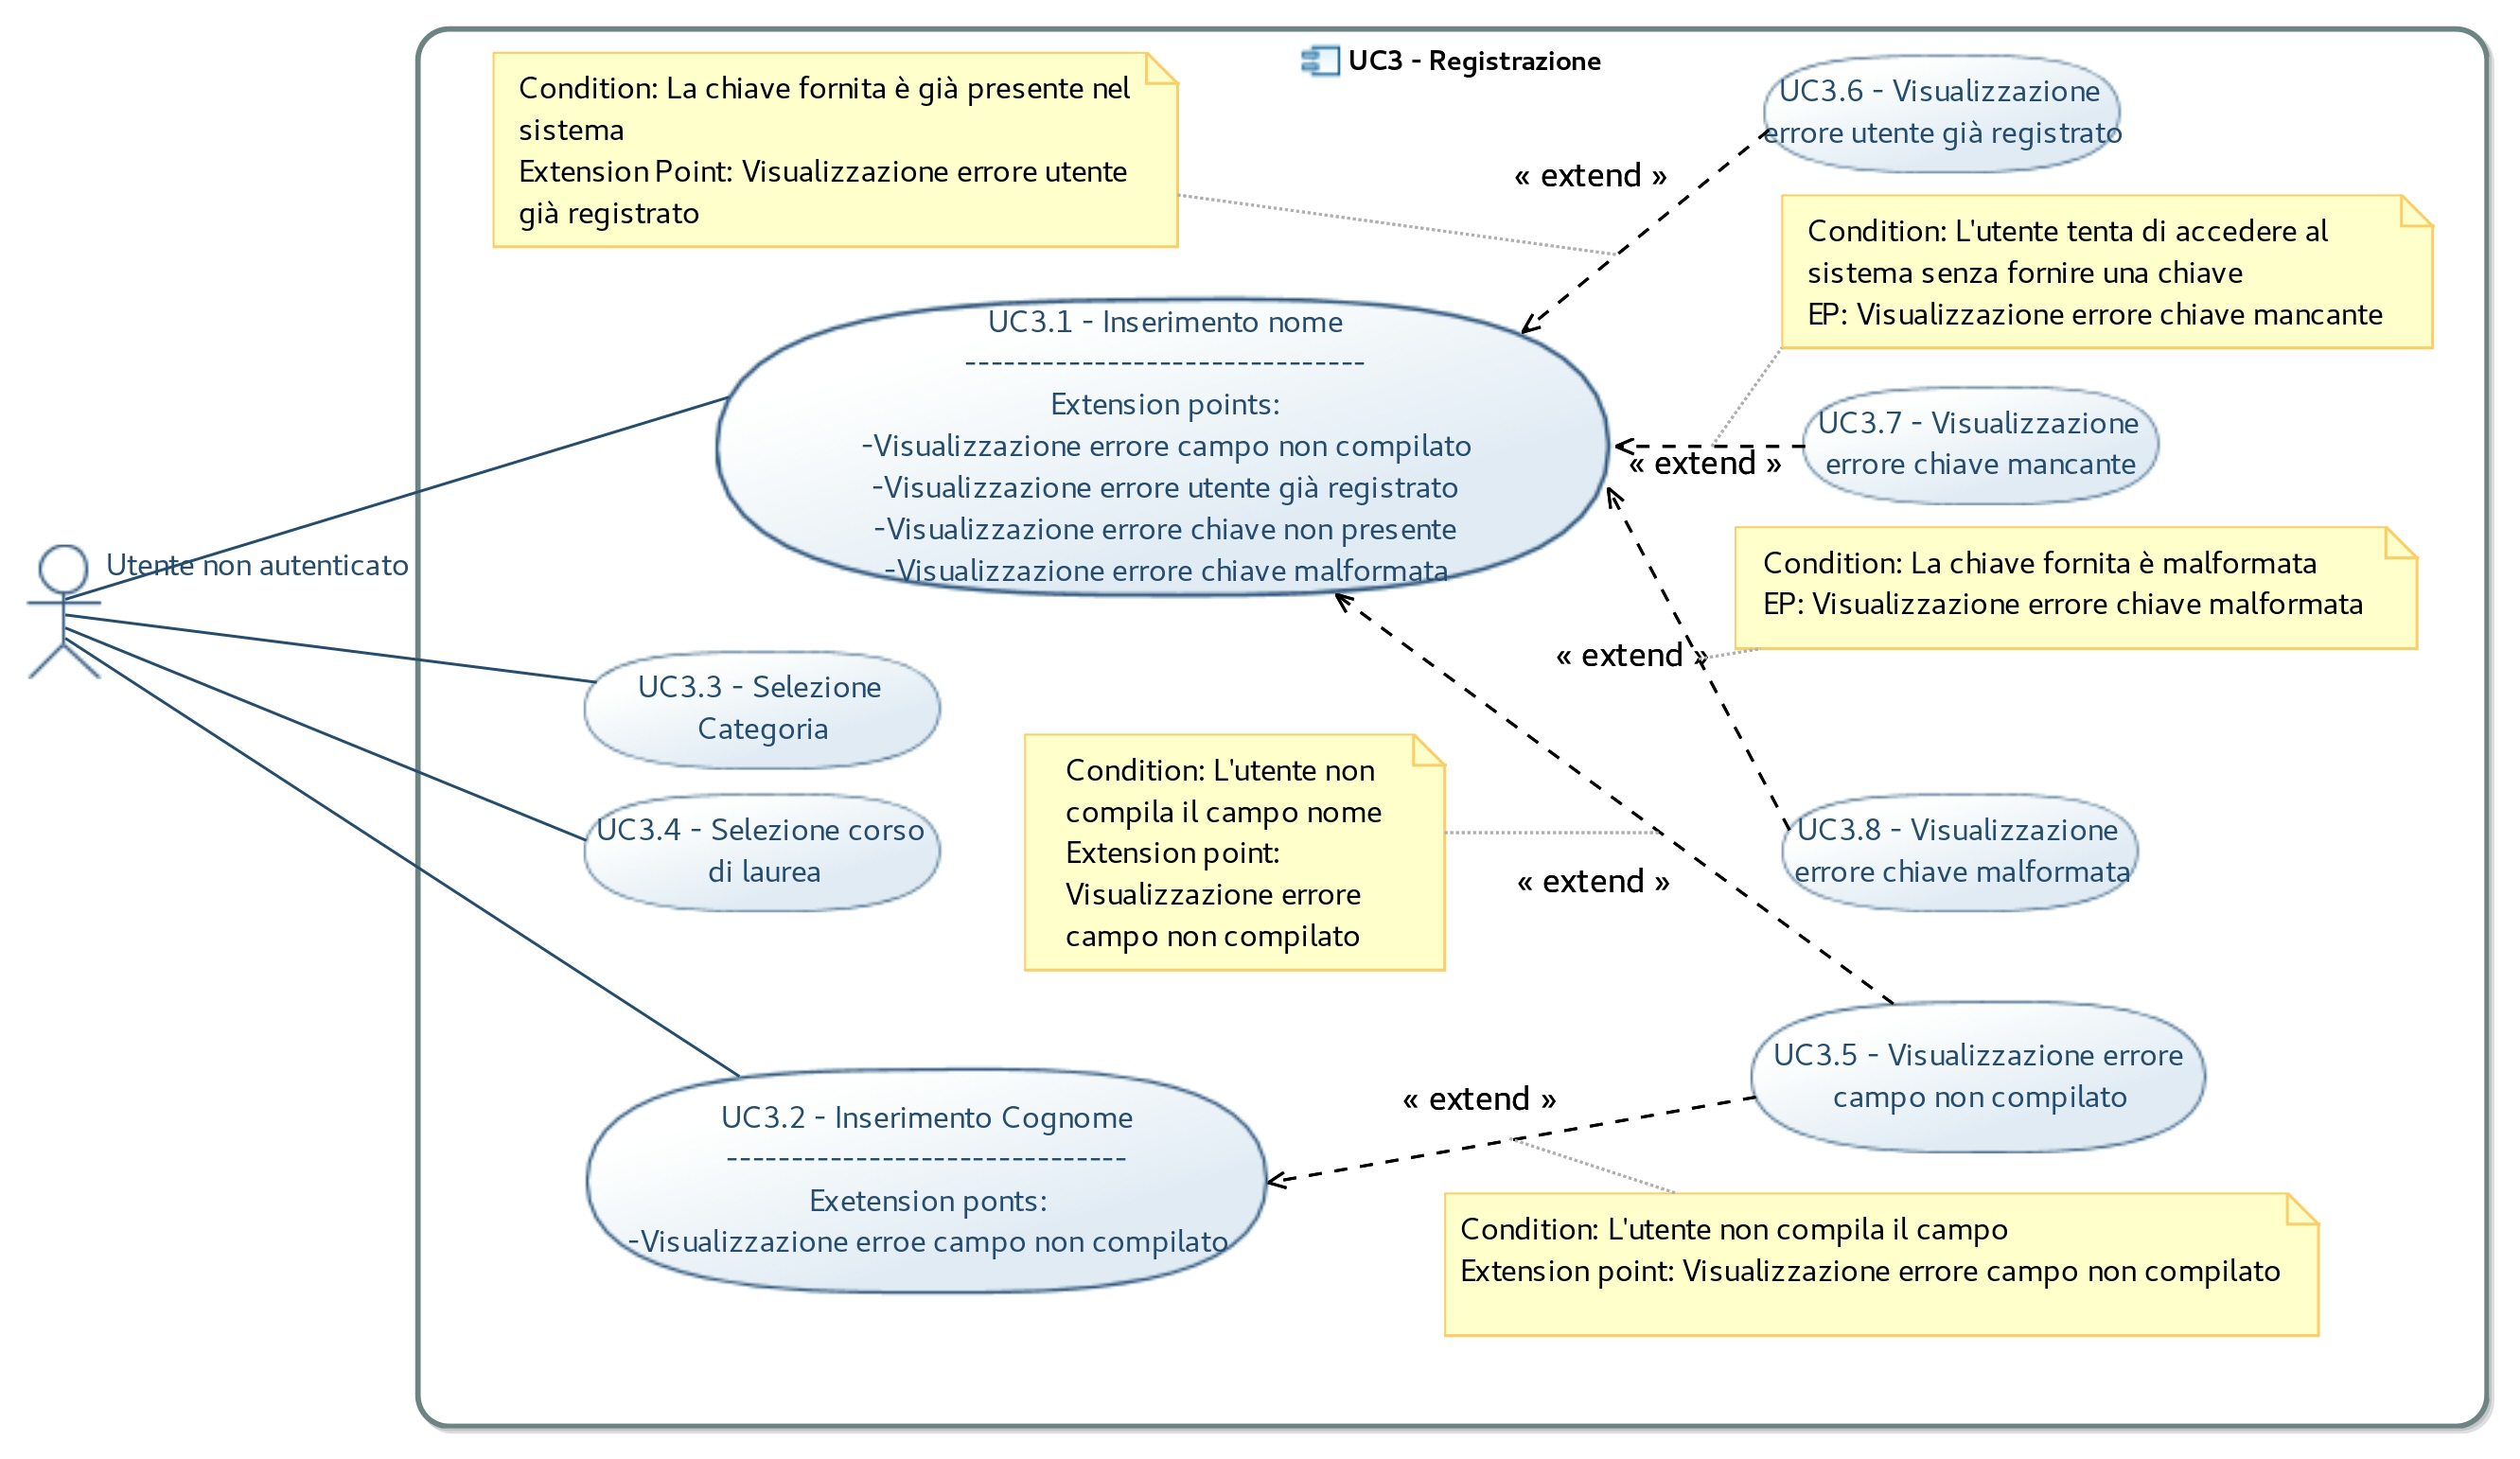
\includegraphics[width=1.0\linewidth]{UC3.jpg}
	\caption{UC3 - Registrazione}
	\label{fig:UC3 - Registrazione}
\end{figure}


\subsection{UC3.1 - Inserimento nome}
\begin{itemize}
	\item \textbf{Attori Primari:} utente non autenticato;
	\item \textbf{Scopo e Descrizione:} il sistema \citGloss{verifica} la validità della \citGloss{chiave} e offre l'interfaccia per inserire il nome dell'utente. Il nome unito al cognome non necessita sia univoco, essendo solamente un' indicazione per facilitare l'identificazione, in quanto a definire univocamente l'account ci pensa la chiave pubblica, che andrà a sostituire la matricola di UniWeb;
	\item \textbf{Scenario principale:} l'utente fornisce tramite un dispositivo di input il suo nome;
	\item \textbf{Estensioni:}
		\begin{enumerate}
			\item Se l'utente non ha un \citGloss{chiave} viene avvisato tramite un messaggio d'errore [UC3.7];
			\item Se l'utente non possiede \citGloss{MetaMask} viene avvisato tramite messaggio d'errore [UC3.8];
			\item Se la \citGloss{chiave} fornita dall'utente è già presente nel sistema l'utente viene avvisato tramite un messaggio d'errore [UC3.6];
			\item Se l'utente non compila il campo viene avvisato con un messaggio d'errore [UC3.5].
		\end{enumerate}
	\item \textbf{Precondizione:} il sistema, che ha ricevuto la richiesta di registrazione da parte dell'utente, fornisce un'interfaccia per l'inserimento del nome e rimane in attesa dell'input;
	\item \textbf{Postcondizione:} il sistema verifica che la \citGloss{chiave} con il quale l'utente sta cercando di registrarsi risulti non utilizzata nel sistema e salva il nome dell'utente.
\end{itemize}	
\subsection{UC3.2 - Inserimento cognome}
\begin{itemize}
	\item \textbf{Attori Primari:} utente non autenticato;
	\item \textbf{Scopo e Descrizione:} il sistema offre l'interfaccia per inserire il cognome dell'utente. Il cognome unito al nome non necessita sia univoco, essendo solamente un' indicazione per facilitare l'identificazione, in quanto a definire univocamente l'account ci pensa la chiave pubblica, che andrà a sostituire la matricola di UniWeb;
	\item \textbf{Scenario principale:} l'utente fornisce tramite un dispositivo di input il suo cognome;
	\item \textbf{Estensioni:}
		\begin{enumerate}
				\item Se l'utente non compila il campo viene avvisato dal sistema [UC3.5].
		\end{enumerate}		
	\item \textbf{Precondizione:} il sistema, che ha ricevuto la richiesta di registrazione da parte dell'utente e ne conosce il nome, fornisce un'interfaccia per l'inserimento del cognome e rimane in attesa dell'input;
	\item \textbf{Postcondizione:} il sistema salva il cognome dell'utente.
\end{itemize}
\subsection{UC3.3 - Selezione categoria}
\begin{itemize}
	\item \textbf{Attori Primari:} utente non autenticato;
	\item \textbf{Scopo e Descrizione:} il sistema offre l'interfaccia per selezionare la categoria di registrazione (studente o professore);
	\item \textbf{Scenario principale:} l'utente seleziona tramite un dispositivo di input la sua categoria;
	\item \textbf{Precondizione:} il sistema, che ha ricevuto la richiesta di registrazione da parte dell'utente e ne conosce il nome e il cognome, fornisce un'interfaccia per la selezione della categoria dell'account che l'utente desidera, a scelta tra professore e studente e rimane in attesa dell'input;
	\item \textbf{Postcondizione:} il sistema salva la categoria nella quale l'utente desidera registrarsi. Se la categoria scelta è quella del professore allora la procedura di registrazione viene terminata e i dati salvati fino a quel momento vengono resi persistenti.
\end{itemize}
\subsection{UC3.4 - Selezione corso di laurea}
\begin{itemize}
	\item \textbf{Attori Primari:} utente non autenticato;
	\item \textbf{Scopo e Descrizione} il sistema offre l'interfaccia per selezionare il \citGloss{corso di laurea} desiderato da un elenco, specificando per ognuno la sigla di riferimento;
	\item \textbf{Scenario principale:} l'utente seleziona tramite un dispositivo di input il \citGloss{corso di laurea} scelto;
	\item \textbf{Precondizione:} il sistema, che ha ricevuto la richiesta di registrazione da parte dell'utente che desidera divenire uno studente, fornisce un'interfaccia per la selezione del \citGloss{corso di laurea} e rimane in attesa dell'input;
	\item \textbf{Postcondizione:} il sistema salva il \citGloss{corso di laurea} nel quale l'utente desidera registrarsi, la procedura di registrazione viene terminata e i dati salvati fino a quel momento vengono resi persistenti.
\end{itemize}

\subsection{UC3.5 - Visualizzazione errore campo non compilato}
\begin{itemize}
	\item \textbf{Attori Primari:} utente non autenticato;
	\item \textbf{Scopo e Descrizione} il sistema avvisa l'utente che non ha compilato il campo selezionato;
	\item \textbf{Scenario principale:} il sistema mostra un messaggio d'errore all'utente che indica la mancata compilazione del campo selezionato;
	\item \textbf{Precondizione:} il sistema ottiene come input da una richiesta di inserimento di un dato una sequenza di caratteri vuota;
	\item \textbf{Postcondizione:} il sistema avvisa l'utente di non aver compilato il campo selezionato.
\end{itemize}
\subsection{UC3.6 - Visualizzazione errore utente già registrato}
\begin{itemize}
	\item \textbf{Attori Primari:} utente non autenticato;
	\item \textbf{Scopo e Descrizione} il sistema avvisa l'utente che la sua \citGloss{chiave} è già presente nel sistema, facendo collidere il suo \citGloss{indirizzo} con uno precedentemente inserito, e che quindi non può procedere alla registrazione;
	\item \textbf{Scenario principale:} il sistema mostra un messaggio d'errore all'utente che indica che sta tentando di effettuare una registrazione utilizzando una \citGloss{chiave} già utilizzata nel sistema;
	\item \textbf{Precondizione:} al sistema viene richiesta una registrazione da parte di un utente che presenta una \citGloss{chiave} precedentemente registrata;
	\item \textbf{Postcondizione:} il sistema avvisa l'utente di star utilizzando una \citGloss{chiave} che corrisponde a un account precedentemente registrato nel sistema.
\end{itemize}
\subsection{UC3.7 - Visualizzazione errore chiave non presente}
\begin{itemize}
	\item \textbf{Attori Primari:} utente non autenticato;
	\item \textbf{Scopo e Descrizione} il sistema avvisa l'utente che non ha fornito una \citGloss{chiave} e quindi non può procedere alla registrazione;
	\item \textbf{Scenario principale:} il sistema mostra un messaggio d'errore all'utente indicandogli l'assenza della \citGloss{chiave};
	\item \textbf{Precondizione:} al sistema viene richiesta una registrazione da parte di un utente che non fornisce una \citGloss{chiave};
	\item \textbf{Postcondizione:} il sistema avvisa l'utente di possedere una \citGloss{chiave} già registrata all'interno del sistema.
\end{itemize}
\subsection{UC3.8 - Visualizzazione errore \citGloss{MetaMask} non installato}
\begin{itemize}
	\item \textbf{Attori Primari:} utente non autenticato;
	\item \textbf{Scopo e Descrizione} il sistema avvisa l'utente del fatto che non possiede il plugin \citGloss{MetaMask};
	\item \textbf{Scenario principale:} il sistema mostra un messaggio d'errore all'utente indicandogli che non ha il plugin \citGloss{MetaMask} installato;
	\item \textbf{Precondizione:} al sistema viene richiesta una registrazione da parte di un utente che non possiede il plugin \citGloss{MetaMask};
	\item \textbf{Postcondizione:} il sistema avvisa l'utente della necessità di dover installare il plugin \citGloss{MetaMask} per potersi registrare.
\end{itemize}
\subsection{UC4 - Logout}
\begin{itemize}
	\item \textbf{Attori primari:} utente autenticato;
	\item \textbf{Scopo e descrizione:} l'utente desidera effettuare il logout dal sistema e gli vengono fornite le istruzioni per effettuarlo, in quanto per completare l'operazione l'utente deve interagire direttamente con il plugin \citGloss{MetaMask};
	\item \textbf{Scenario principale:} l'utente autenticato richiede il logout dal sistema;
	\item \textbf{Precondizione:} il sistema riconosce l'utente come autenticato e riceve una richiesta di logout;
	\item \textbf{Postcondizione:} il sistema informa l'utente riguardo alla modalità di logout dal sistema.
\end{itemize}

\subsection{UC5 - Gestione Utenti}
\begin{itemize}
	\item \textbf{Attori primari:} amministratore;
	\item \textbf{Scopo e descrizione:} l'amministratore è in grado di eseguire operazioni sugli utenti all'interno dell'ateneo che presentano account registrati o in attesa di registrazione nel ruolo di studenti o professori;
	\item \textbf{Scenario principale:} l'amministratore visualizza una lista di operazioni eseguibili sugli utenti appartenenti alla categoria dei professori o degli studenti e sceglie quale effettuare;
	\item \textbf{Precondizione:} il sistema riconosce l'utente nel ruolo di amministratore e mette a disposizione una serie di strumenti per la manipolazione degli utenti; 
	\item \textbf{Postcondizione:} il sistema effettua le operazioni richieste riguardanti la gestione degli utenti.
\end{itemize}
\begin{figure}[H]
	\centering
	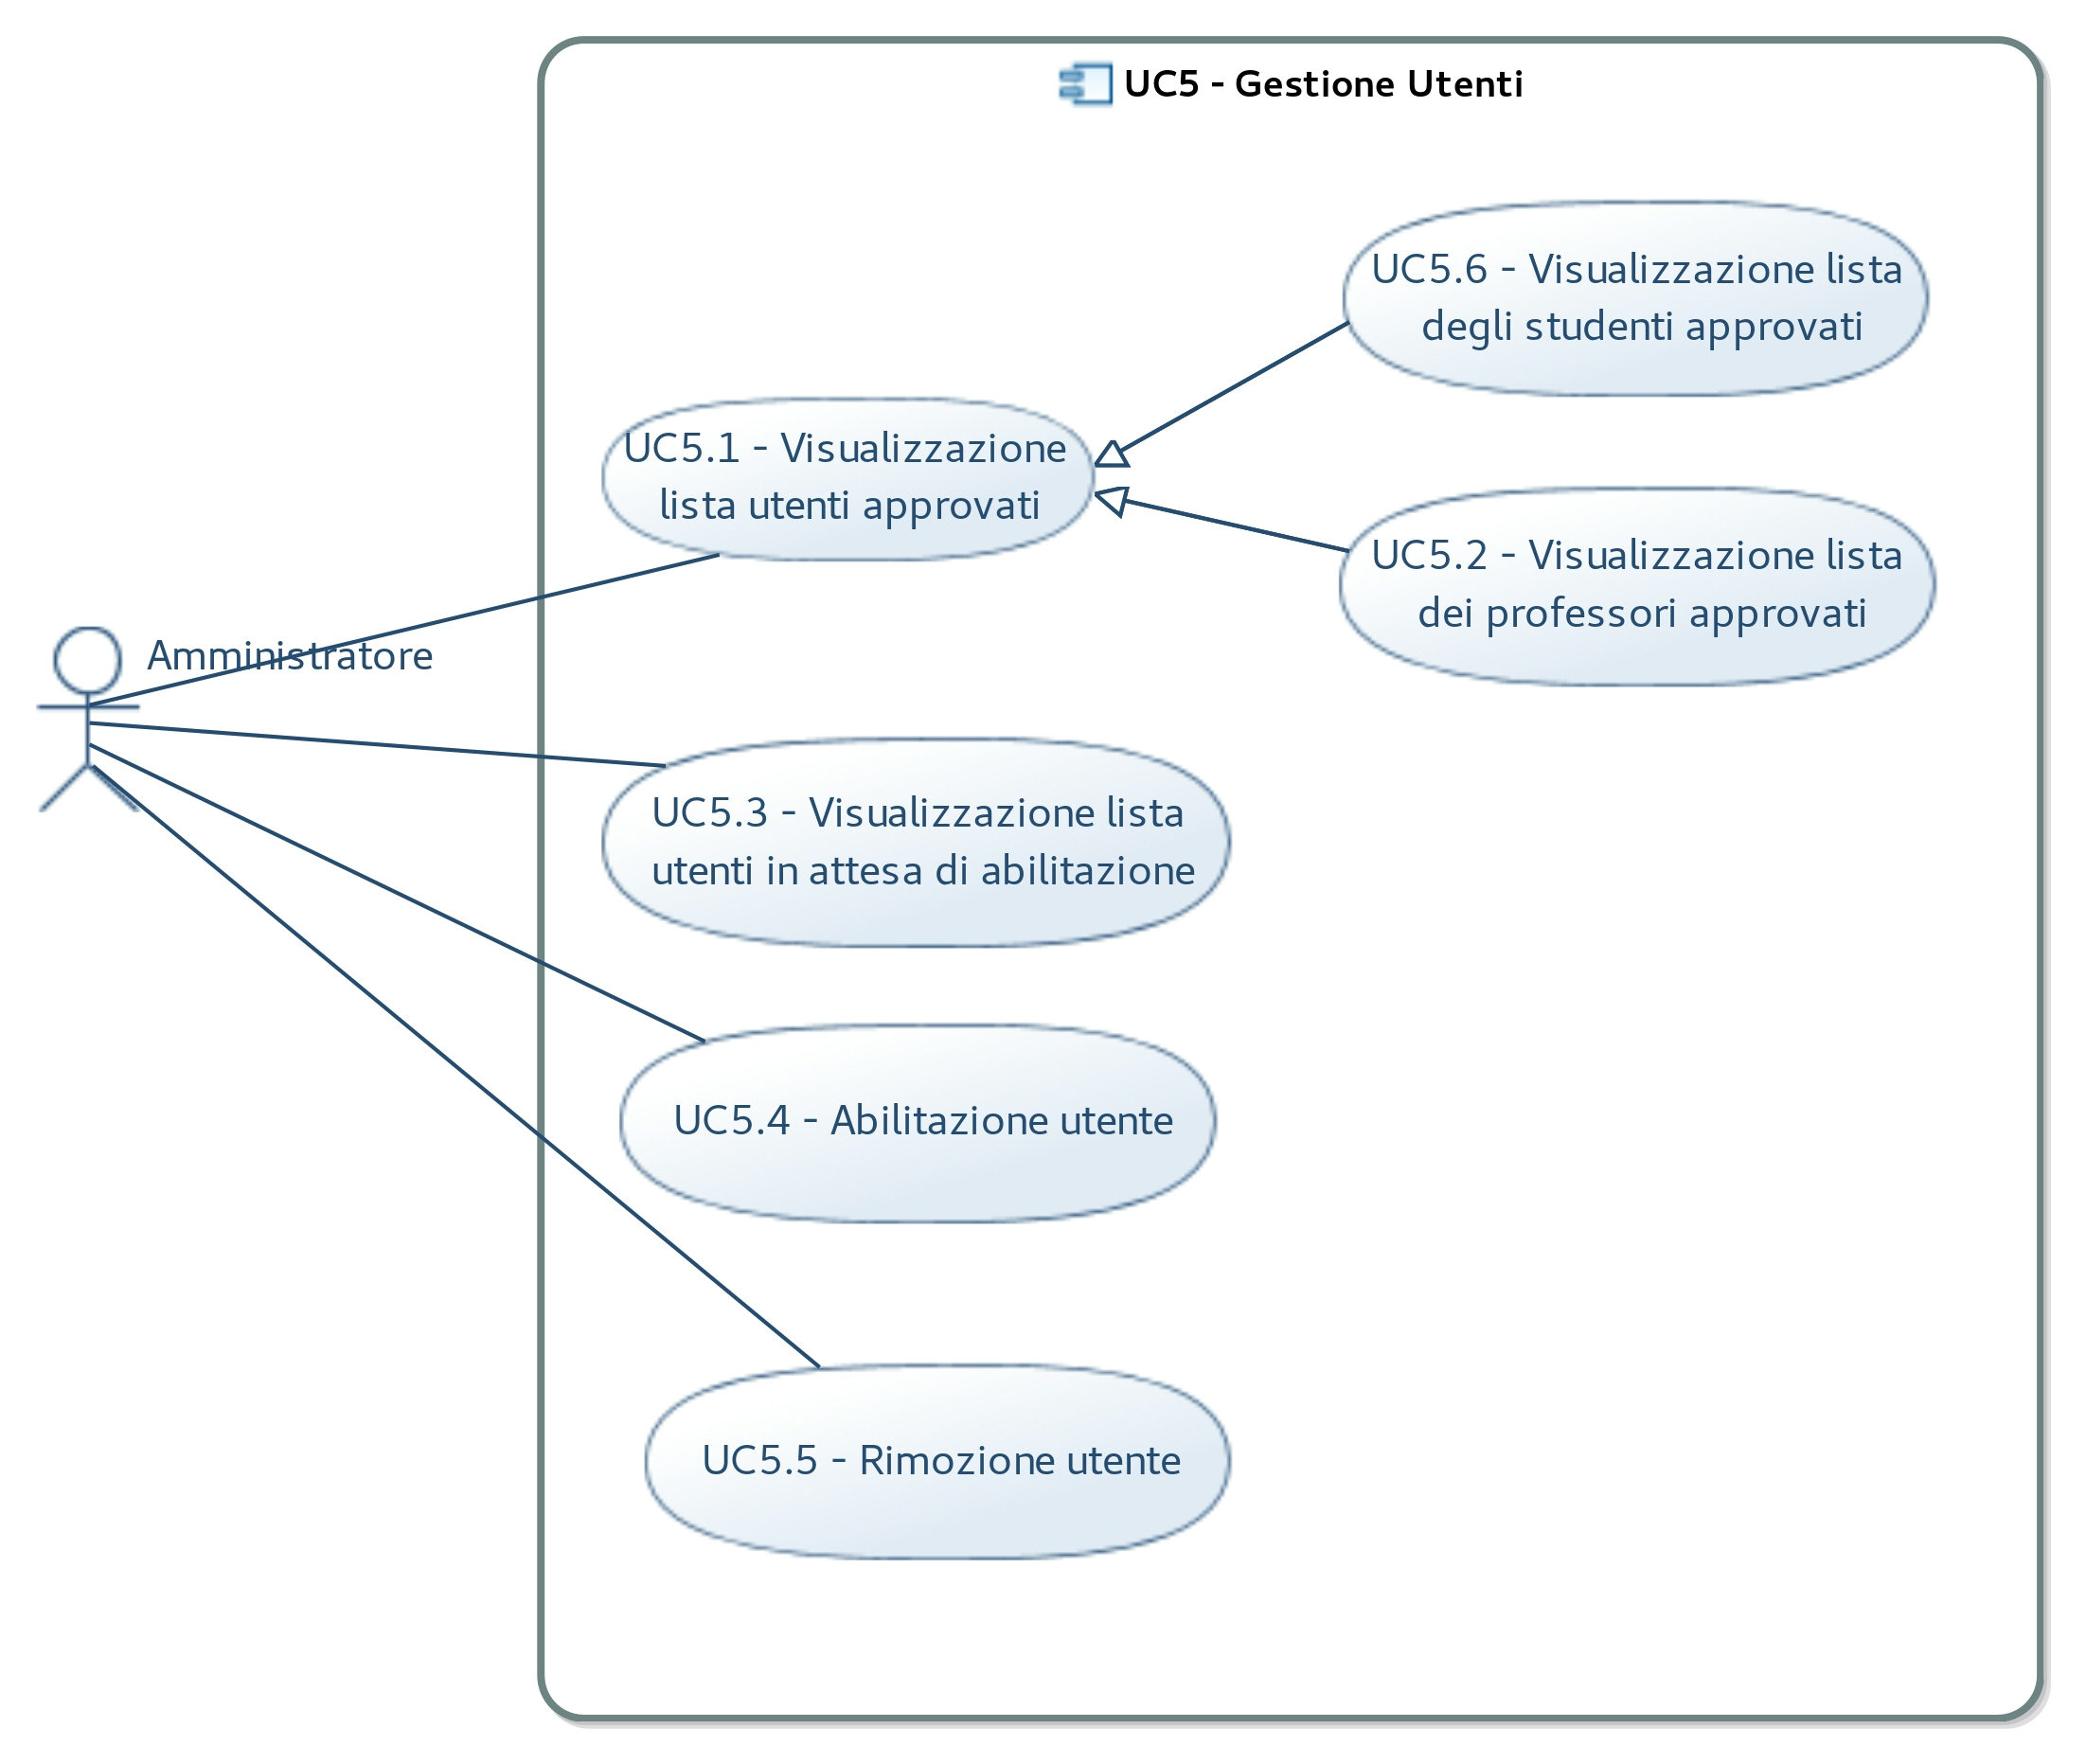
\includegraphics[width=0.8\linewidth]{UC5.jpg}
	\caption{UC5 - Gestione Utenti}
	\label{fig:UC5 - Gestione Utenti}
\end{figure}
\subsection{UC5.1 - Visualizzazione lista degli utenti approvati}
\begin{itemize}
	\item \textbf{Attori primari:} amministratore;
	\item \textbf{Scopo e descrizione:} l'amministratore visualizza una lista di tutti gli utenti registrati nel sistema, visualizzando per ognuno di essi le informazioni basilari;
	\item \textbf{Scenario principale:} l'amministratore richiede al sistema una lista di utenti per poterli visualizzare ed eventualmente compiere altre operazioni su di essi;
	\item \textbf{Specializzazioni:}
	\begin{enumerate}
		\item UC5.2 - Visualizzazione lista degli studenti approvati;
		\item UC5.3 - Visualizzazione lista dei professori approvati.
	\end{enumerate}
	\item \textbf{Precondizione:} il sistema riconosce l'utente nel ruolo di amministratore; 
	\item \textbf{Postcondizione:} il sistema offre all'amministratore la lista degli utenti approvati.
\end{itemize}
\begin{figure}[H]
	\centering
	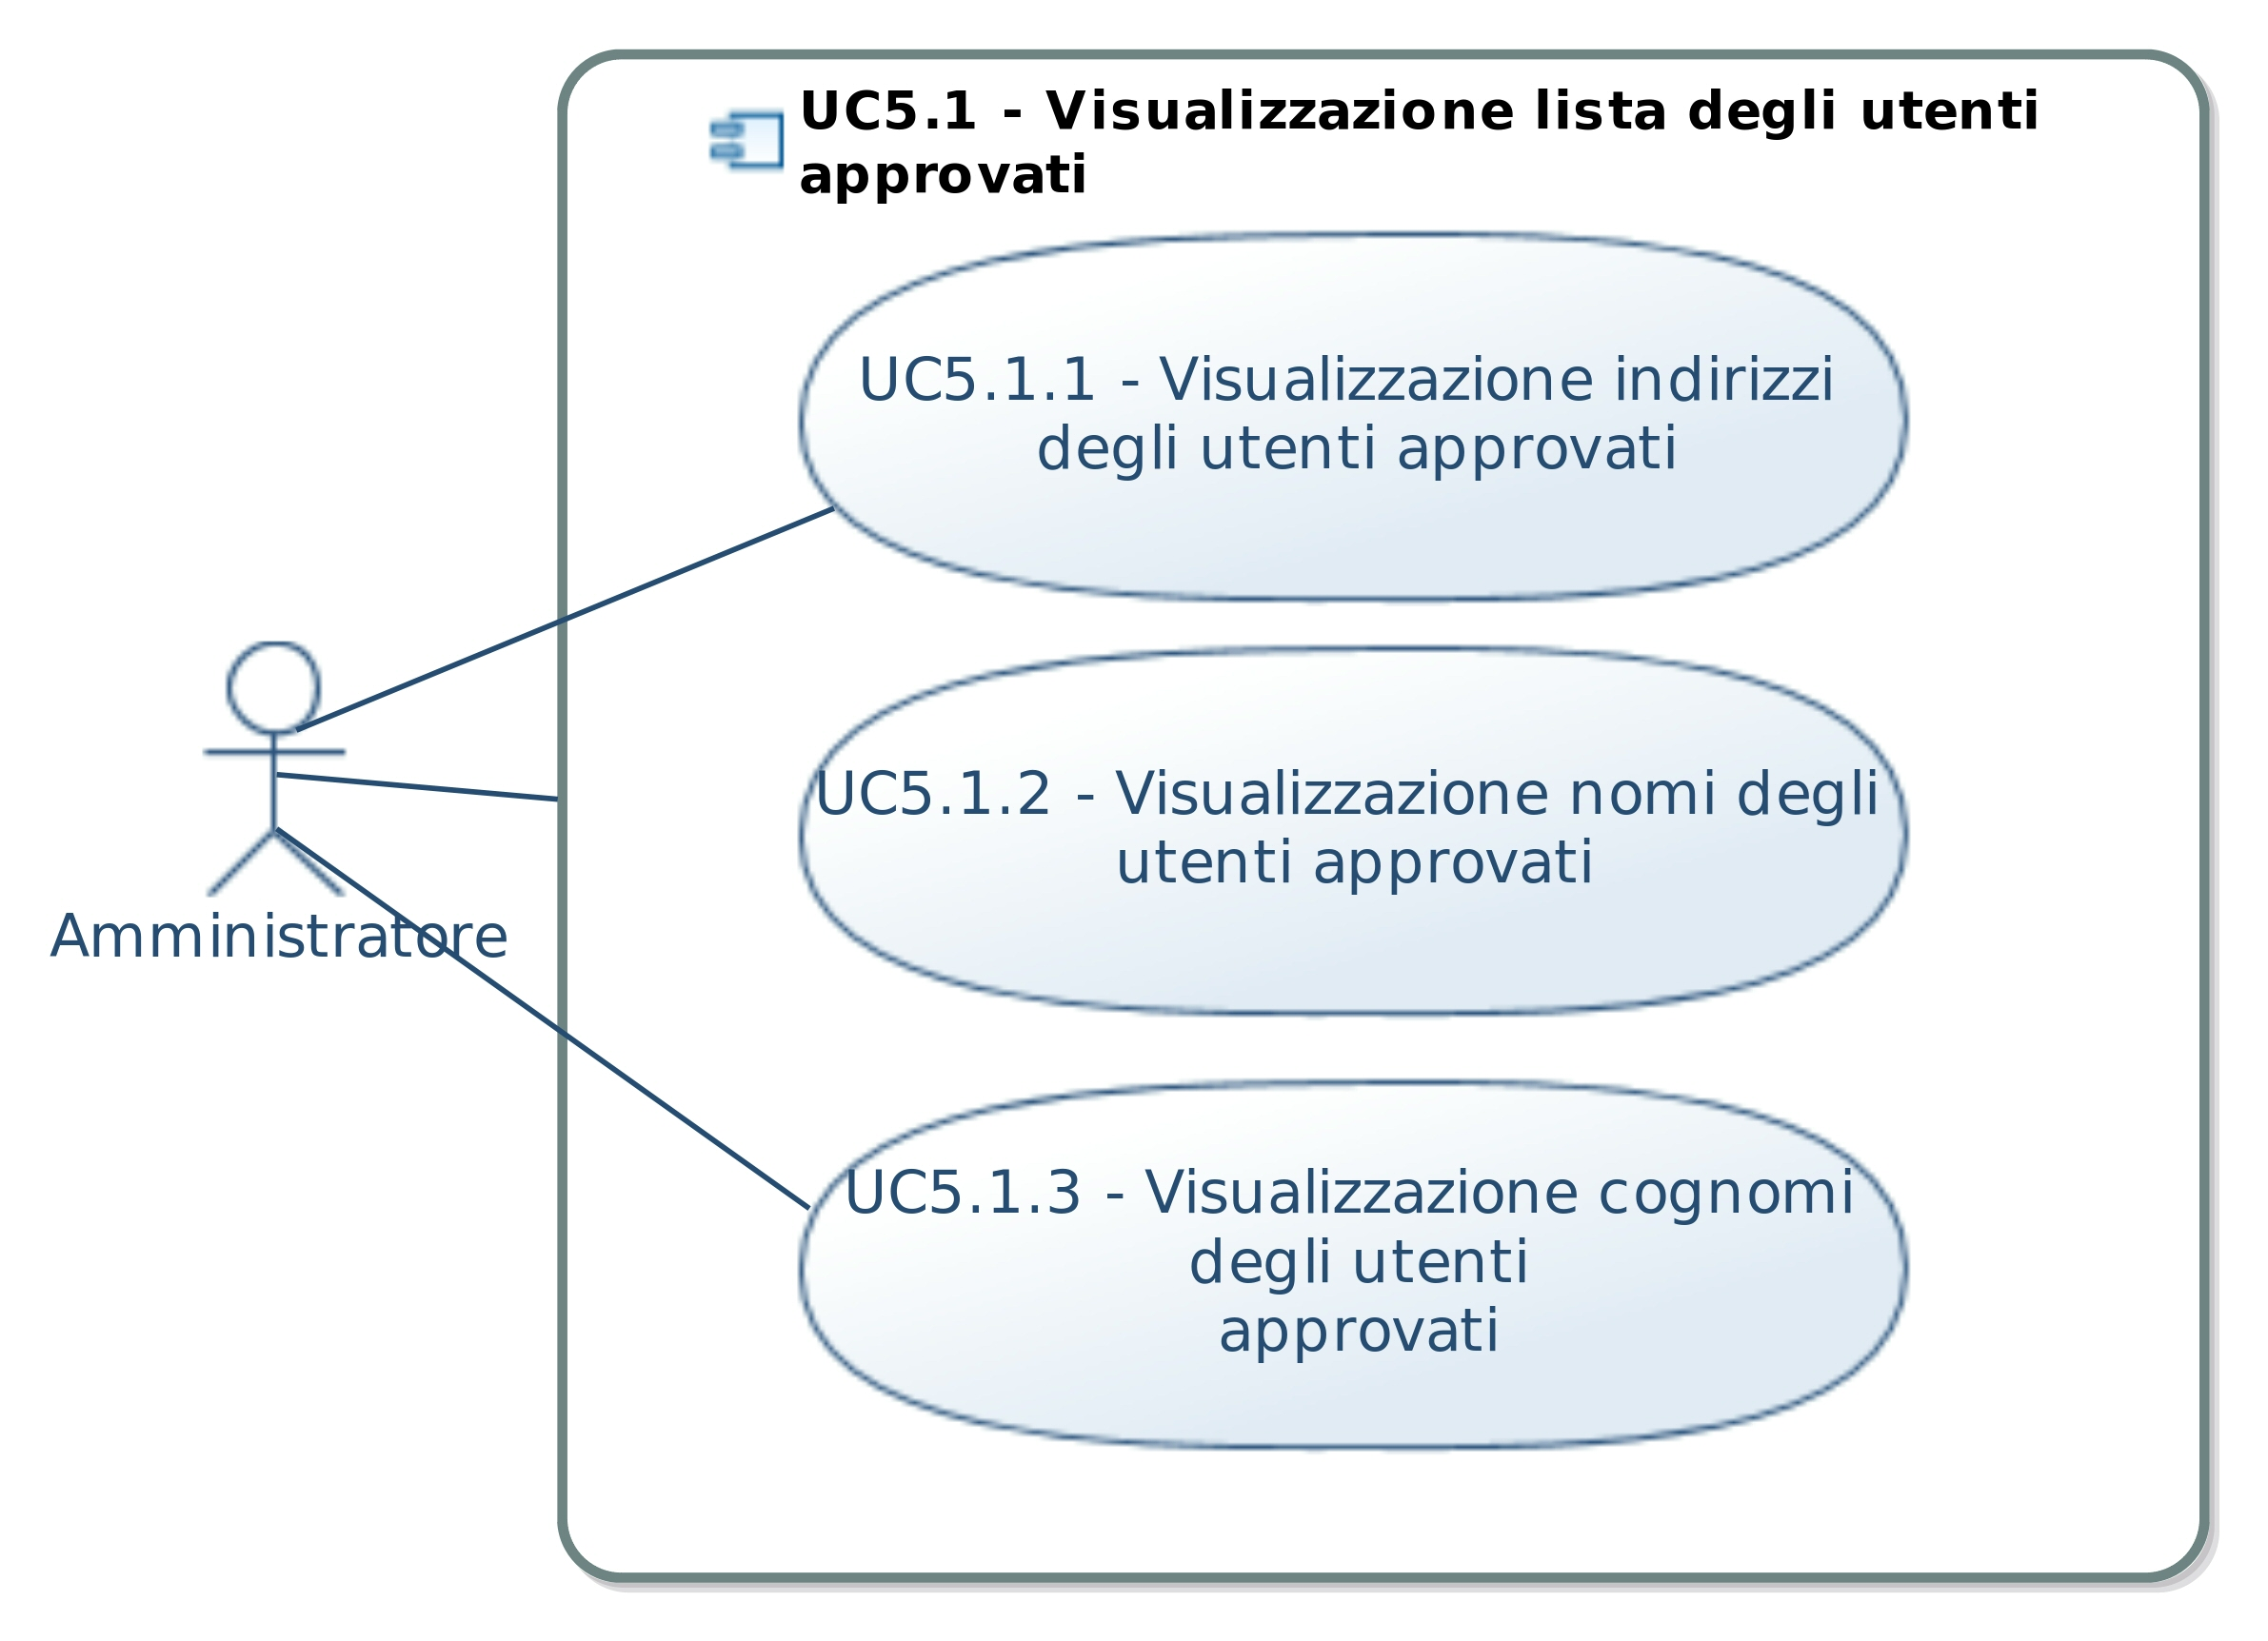
\includegraphics[width=0.9\linewidth]{UC5_1.jpg}
	\caption{UC5.1 - Visualizzazione lista degli utenti approvati}
	\label{fig:UC5.1 - Visualizzazione lista degli utenti approvati}
\end{figure}
\subsection{UC5.1.1 - Visualizzazione indirizzi degli utenti approvati}
\begin{itemize}
	\item \textbf{Attori primari:} amministratore;
	\item \textbf{Scopo e descrizione:} l'amministratore visualizza una lista di tutti gli \citGloss{indirizzi} della rete \citGloss{Ethereum} degli utenti registrati nel sistema;
	\item \textbf{Scenario principale:} l'amministratore richiede al sistema una lista di utenti per poterne visualizzare l'\citGloss{indirizzo} ed eventualmente compiere altre operazioni su di essi;
	\item \textbf{Precondizione:} il sistema riconosce l'utente nel ruolo di amministratore e riceve la richiesta di visualizzazione della lista degli utenti approvati;
	\item \textbf{Postcondizione:} il sistema offre all'amministratore la lista degli utenti approvati con indicati gli \citGloss{indirizzi}.
\end{itemize}
\subsection{UC5.1.2 - Visualizzazione nomi degli utenti approvati}
\begin{itemize}
	\item \textbf{Attori primari:} amministratore;
	\item \textbf{Scopo e descrizione:} l'amministratore visualizza una lista di tutti i nomi degli utenti registrati nel sistema;
	\item \textbf{Scenario principale:} l'amministratore richiede al sistema una lista di utenti per poterne visualizzare il nome ed eventualmente compiere altre operazioni su di essi;
	\item \textbf{Precondizione:} il sistema riconosce l'utente nel ruolo di amministratore e riceve la richiesta di visualizzazione della lista degli utenti approvati;
	\item \textbf{Postcondizione:} il sistema offre all'amministratore la lista degli utenti approvati con indicati i nomi.
\end{itemize}
\subsection{UC5.1.3 - Visualizzazione cognomi degli utenti approvati}
\begin{itemize}
	\item \textbf{Attori primari:} amministratore;
	\item \textbf{Scopo e descrizione:} l'amministratore visualizza una lista di tutti i cognomi degli utenti registrati nel sistema;
	\item \textbf{Scenario principale:} l'amministratore richiede al sistema una lista di utenti per poterne visualizzare il cognome ed eventualmente compiere altre operazioni su di essi;
	\item \textbf{Precondizione:} il sistema riconosce l'utente nel ruolo di amministratore e riceve la richiesta di visualizzazione della lista degli utenti approvati;
	\item \textbf{Postcondizione:} il sistema offre all'amministratore la lista degli utenti approvati con indicati i cognomi.
\end{itemize}
\subsection{UC5.2 - Visualizzazione lista degli studenti approvati}
\begin{itemize}
	\item \textbf{Attori primari:} amministratore;
	\item \textbf{Scopo e descrizione:} l'amministratore visualizza una lista di tutti gli studenti registrati nel sistema, visualizzando per ognuno di essi le informazioni basilari;
	\item \textbf{Scenario principale:} l'amministratore richiede al sistema una lista di studenti per poterli visualizzare ed eventualmente compiere altre operazioni su di essi;
	\item \textbf{Use case padre:} UC5.1 - Visualizzazione lista degli utenti approvati;
	\item \textbf{Precondizione:} il sistema riconosce l'utente nel ruolo di amministratore; 
	\item \textbf{Postcondizione:} il sistema offre all'amministratore la lista degli studenti approvati.
\end{itemize}
\begin{figure}[H]
	\centering
	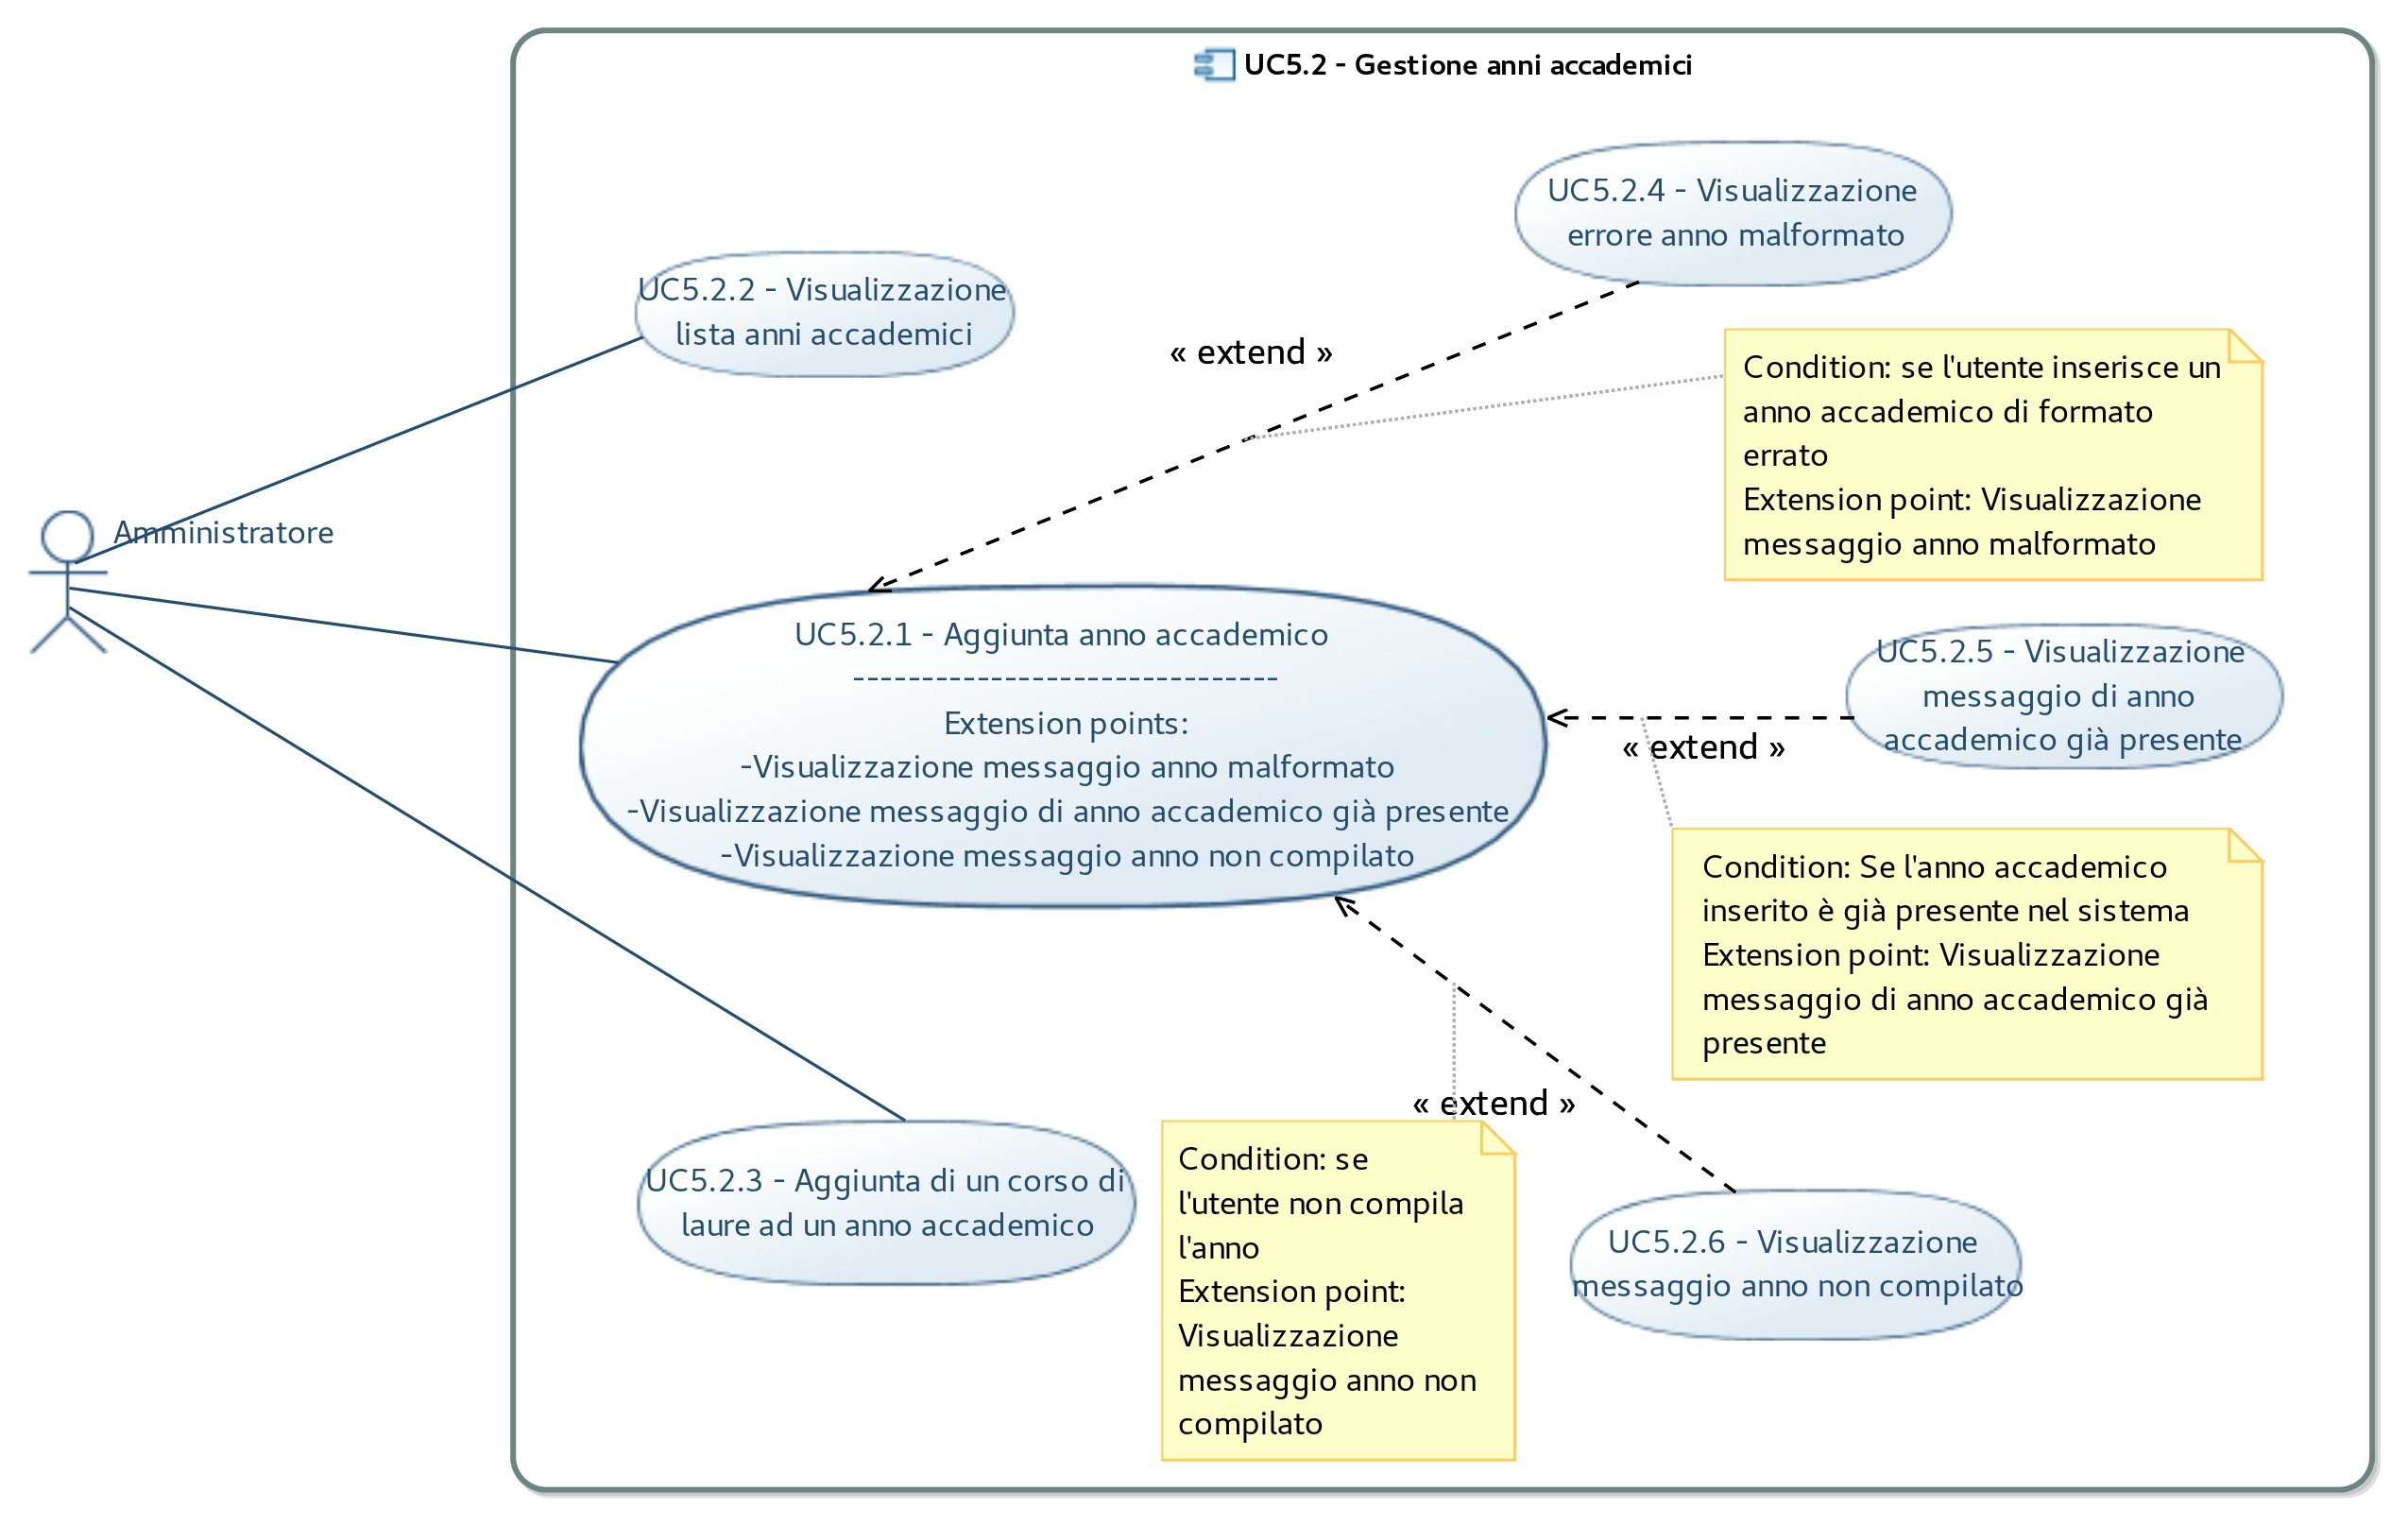
\includegraphics[width=0.9\linewidth]{UC5_2.jpg}
	\caption{UC5.2 - Visualizzazione lista degli studenti approvati}
	\label{fig:UC5.2 - Visualizzazione lista degli studenti approvati}
\end{figure}
\subsection{UC5.2.1 - Visualizzazione nomi dei corsi degli studenti approvati}
\begin{itemize}
	\item \textbf{Attori primari:} amministratore;
	\item \textbf{Scopo e descrizione:} l'amministratore visualizza una lista di tutti gli studenti registrati nel sistema con indicato il nome del relativo corso universitario;
	\item \textbf{Scenario principale:} l'amministratore richiede al sistema una lista di studenti per poterne visualizzare il nome del corso universitario ed eventualmente compiere altre operazioni su di essi;
	\item \textbf{Precondizione:} il sistema riconosce l'utente nel ruolo di amministratore e riceve la richiesta di visualizzazione della lista degli studenti approvati;
	\item \textbf{Postcondizione:} il sistema offre all'amministratore la lista degli studenti approvati con indicati i nomi dei corsi di laurea.
\end{itemize}
\subsection{UC5.3 - Visualizzazione lista dei professori approvati}
\begin{itemize}
	\item \textbf{Attori primari:} amministratore;
	\item \textbf{Scopo e descrizione:} l'amministratore visualizza una lista di tutti i professori registrati nel sistema, visualizzando per ognuno di essi le informazioni basilari;
	\item \textbf{Scenario principale:} l'amministratore richiede al sistema una lista di professori per poterli visualizzare ed eventualmente compiere altre operazioni su di essi;
	\item \textbf{Use case padre:} UC5.1 - Visualizzazione lista degli utenti approvati;
	\item \textbf{Precondizione:} il sistema riconosce l'utente nel ruolo di amministratore; 
	\item \textbf{Postcondizione:} il sistema offre all'amministratore la lista dei professori approvati.
\end{itemize}
\subsection{UC5.4 - Visualizzazione lista utenti in attesa di abilitazione}
\begin{itemize}
	\item \textbf{Attori primari:} amministratore;
	\item \textbf{Scopo e descrizione:} l'amministratore visualizza una lista di tutti gli utenti ancora non abilitati, ottenendo per ognuno tutte le informazioni utili;
	\item \textbf{Scenario principale:} l'amministratore richiede al sistema una lista di utenti in attesa di abilitazione per poterli visualizzare ed eventualmente compiere altre operazioni su di essi;
	\item \textbf{Precondizione:} il sistema riconosce l'utente nel ruolo di amministratore; 
	\item \textbf{Postcondizione:} il sistema offre all'amministratore la lista degli utenti in attesa di approvazione.
\end{itemize}
\begin{figure}[H]
	\centering
	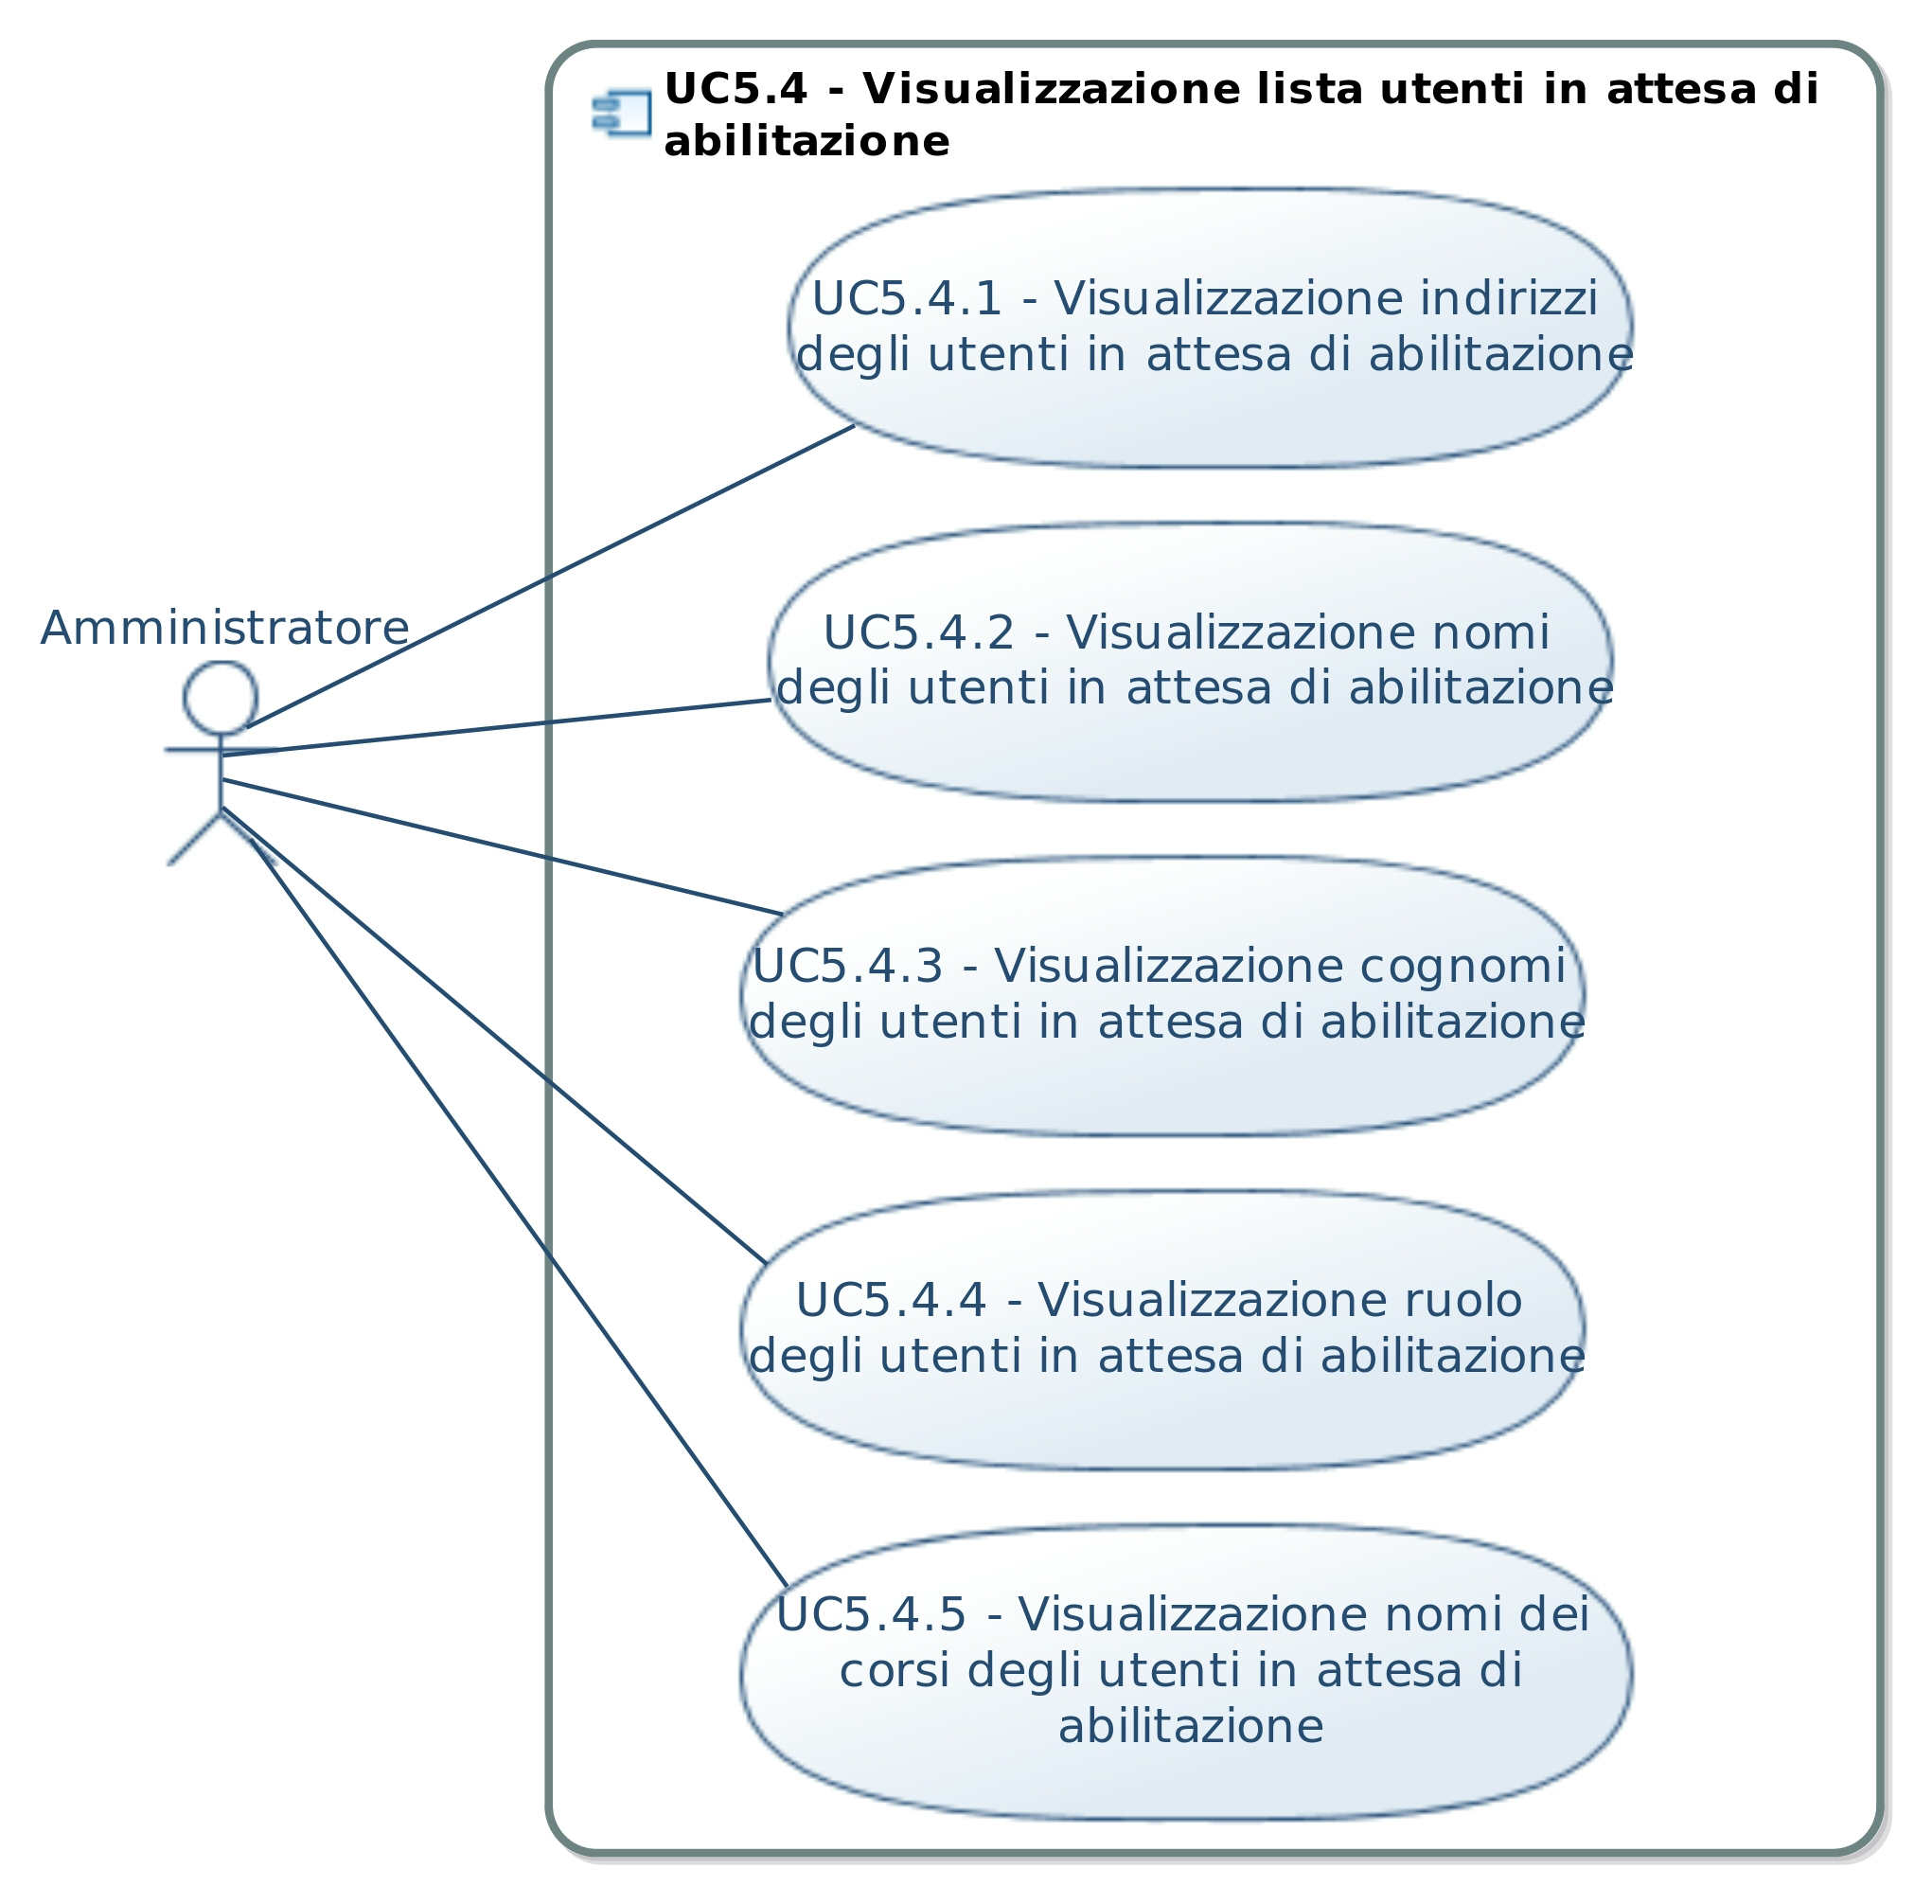
\includegraphics[width=0.8\linewidth]{UC5_4.jpg}
	\caption{UC5.4 - Visualizzazione lista utenti in attesa di abilitazione}
	\label{fig:UC5.4 - Visualizzazione lista utenti in attesa di abilitazione}
\end{figure}
\subsection{UC5.4.1 - Visualizzazione indirizzi degli utenti in attesa di abilitazione}
\begin{itemize}
	\item \textbf{Attori primari:} amministratore;
	\item \textbf{Scopo e descrizione:} l'amministratore visualizza una lista di tutti gli \citGloss{indirizzi} della rete \citGloss{Ethereum} degli utenti in attesa di abilitazione;
	\item \textbf{Scenario principale:} l'amministratore richiede al sistema una lista degli utenti in attesa di abilitazione per poterne visualizzare l'\citGloss{indirizzo} ed eventualmente compiere altre operazioni su di essi;
	\item \textbf{Precondizione:} il sistema riconosce l'utente nel ruolo di amministratore e riceve la richiesta di visualizzazione della lista degli utenti in attesa di approvazione;
	\item \textbf{Postcondizione:} il sistema offre all'amministratore la lista degli utenti in attesa di approvazione con indicati gli \citGloss{indirizzi}.
\end{itemize}
\subsection{UC5.4.2 - Visualizzazione nomi degli utenti in attesa di abilitazione}
\begin{itemize}
	\item \textbf{Attori primari:} amministratore;
	\item \textbf{Scopo e descrizione:} l'amministratore visualizza una lista di tutti i nomi degli utenti in attesa di abilitazione;
	\item \textbf{Scenario principale:} l'amministratore richiede al sistema una lista degli utenti in attesa di abilitazione per poterne visualizzare il nome ed eventualmente compiere altre operazioni su di essi;
	\item \textbf{Precondizione:} il sistema riconosce l'utente nel ruolo di amministratore e riceve la richiesta di visualizzazione della lista degli utenti in attesa di approvazione;
	\item \textbf{Postcondizione:} il sistema offre all'amministratore la lista degli utenti in attesa di approvazione con indicati i nomi.
\end{itemize}
\subsection{UC5.4.3 - Visualizzazione cognomi degli utenti in attesa di abilitazione}
\begin{itemize}
	\item \textbf{Attori primari:} amministratore;
	\item \textbf{Scopo e descrizione:} l'amministratore visualizza una lista di tutti i cognomi degli utenti in attesa di abilitazione;
	\item \textbf{Scenario principale:} l'amministratore richiede al sistema una lista degli utenti in attesa di abilitazione per poterne visualizzare il cognome ed eventualmente compiere altre operazioni su di essi;
	\item \textbf{Precondizione:} il sistema riconosce l'utente nel ruolo di amministratore e riceve la richiesta di visualizzazione della lista degli utenti in attesa di approvazione;
	\item \textbf{Postcondizione:} il sistema offre all'amministratore la lista degli utenti in attesa di approvazione con indicati i cognomi.
\end{itemize}
\subsection{UC5.4.4 - Visualizzazione ruolo degli utenti in attesa di abilitazione}
\begin{itemize}
	\item \textbf{Attori primari:} amministratore;
	\item \textbf{Scopo e descrizione:} l'amministratore visualizza una lista degli utenti in attesa di abilitazione e i relativi ruoli che desiderano ricoprire una volta approvati, cioè professori o studenti;
	\item \textbf{Scenario principale:} l'amministratore richiede al sistema una lista degli utenti in attesa di abilitazione per poterne visualizzare il ruolo desiderato ed eventualmente compiere altre operazioni su di essi;
	\item \textbf{Precondizione:} il sistema riconosce l'utente nel ruolo di amministratore e riceve la richiesta di visualizzazione della lista degli utenti in attesa di approvazione;
	\item \textbf{Postcondizione:} il sistema offre all'amministratore la lista degli utenti in attesa di approvazione con indicati i ruoli che desiderano ottenere.
\end{itemize}
\subsection{UC5.4.5 - Visualizzazione nomi dei corsi degli utenti in attesa di abilitazione}
\begin{itemize}
	\item \textbf{Attori primari:} amministratore;
	\item \textbf{Scopo e descrizione:} l'amministratore visualizza una lista di tutti gli utenti in attesa di abilitazione con indicato il nome del relativo corso universitario nel caso l'utente abbia richiesto di essere uno studente;
	\item \textbf{Scenario principale:} l'amministratore richiede al sistema una lista degli utenti in attesa di abilitazione per poterne visualizzare il nome del corso universitario ove possibile ed eventualmente compiere altre operazioni su di essi;
	\item \textbf{Precondizione:} il sistema riconosce l'utente nel ruolo di amministratore e riceve la richiesta di visualizzazione della lista degli utenti in attesa di approvazione;
	\item \textbf{Postcondizione:} il sistema offre all'amministratore la lista degli utenti in attesa di approvazione con indicati i nomi relativi ai corsi universitari ai quali desiderano partecipare nel caso si tratti di studenti, altrimenti viene restituito un campo vuoto.
\end{itemize}
\subsection{UC5.5 - Abilitazione utente}
\begin{itemize}
	\item \textbf{Attori primari:} amministratore;
	\item \textbf{Scopo e descrizione:} l'amministratore abilita la registrazione di un utente;
	\item \textbf{Scenario principale:}
	\begin{enumerate}
		\item L'amministratore visualizza la lista degli utenti in attesa di abilitazione [UC7];
		\item L'amministratore lo abilita [UC5.5].
	\end{enumerate}
	\item \textbf{Precondizione:} il sistema riconosce l'utente nel ruolo di amministratore e gli ha precedentemente fornito la lista degli utenti in attesa di abilitazione [UC5.4];
	\item \textbf{Postcondizione:} il sistema abilita un utente, rimuovendolo dalla lista degli utenti in attesa di abilitazione e aggiungendolo alla relativa lista degli utenti abilitati.
\end{itemize}
\subsection{UC5.6 - Rimozione utente}
\begin{itemize}
	\item \textbf{Attori primari:} amministratore;
	\item \textbf{Scopo e descrizione:} l'amministratore rimuove dal sistema un utente non ancora abilitato o già abilitato;
	\item \textbf{Scenario principale:}
	\begin{enumerate}
		\item L'amministratore visualizza gli utenti abilitati o in attesa di abilitazione e ne seleziona uno [UC5.1 o UC6 o UC7];
		\item L'amministratore rimuove l'utente selezionato [UC5.6].
	\end{enumerate}
	\item \textbf{Precondizione:} il sistema riconosce l'utente nel ruolo di amministratore e gli ha precedentemente fornito la lista degli utenti, di qualsiasi genere [UC5.1, UC5.3, UC5.4];
	\item \textbf{Postcondizione:} il sistema rimuove l'utente indicato dall'amministratore.
\end{itemize}

\subsection{UC6 - Gestione anni accademici}
\begin{itemize}
	\item \textbf{Attori primari:} università;
	\item \textbf{Scopo e descrizione:} l'utente è già riconosciuto dal sistema come rappresentante dell'università ed è in grado di eseguire operazioni di amministrazione riguardanti gli anni accademici dell'ateneo;
	\item \textbf{Scenario principale:} l'utente che rappresenta l'università visualizza una lista di operazioni eseguibili sugli anni accademici e ne sceglie una;
	\item \textbf{Precondizione:} il sistema riconosce l'utente nel ruolo di rappresentante dell'università e mette a disposizione una serie di operazioni atte alla gestione degli anni accademici; 
	\item \textbf{Postcondizione:} il sistema effettua le operazioni richieste riguardanti la gestione degli anni accademici.
\end{itemize}

\begin{figure}[H]
	\centering
	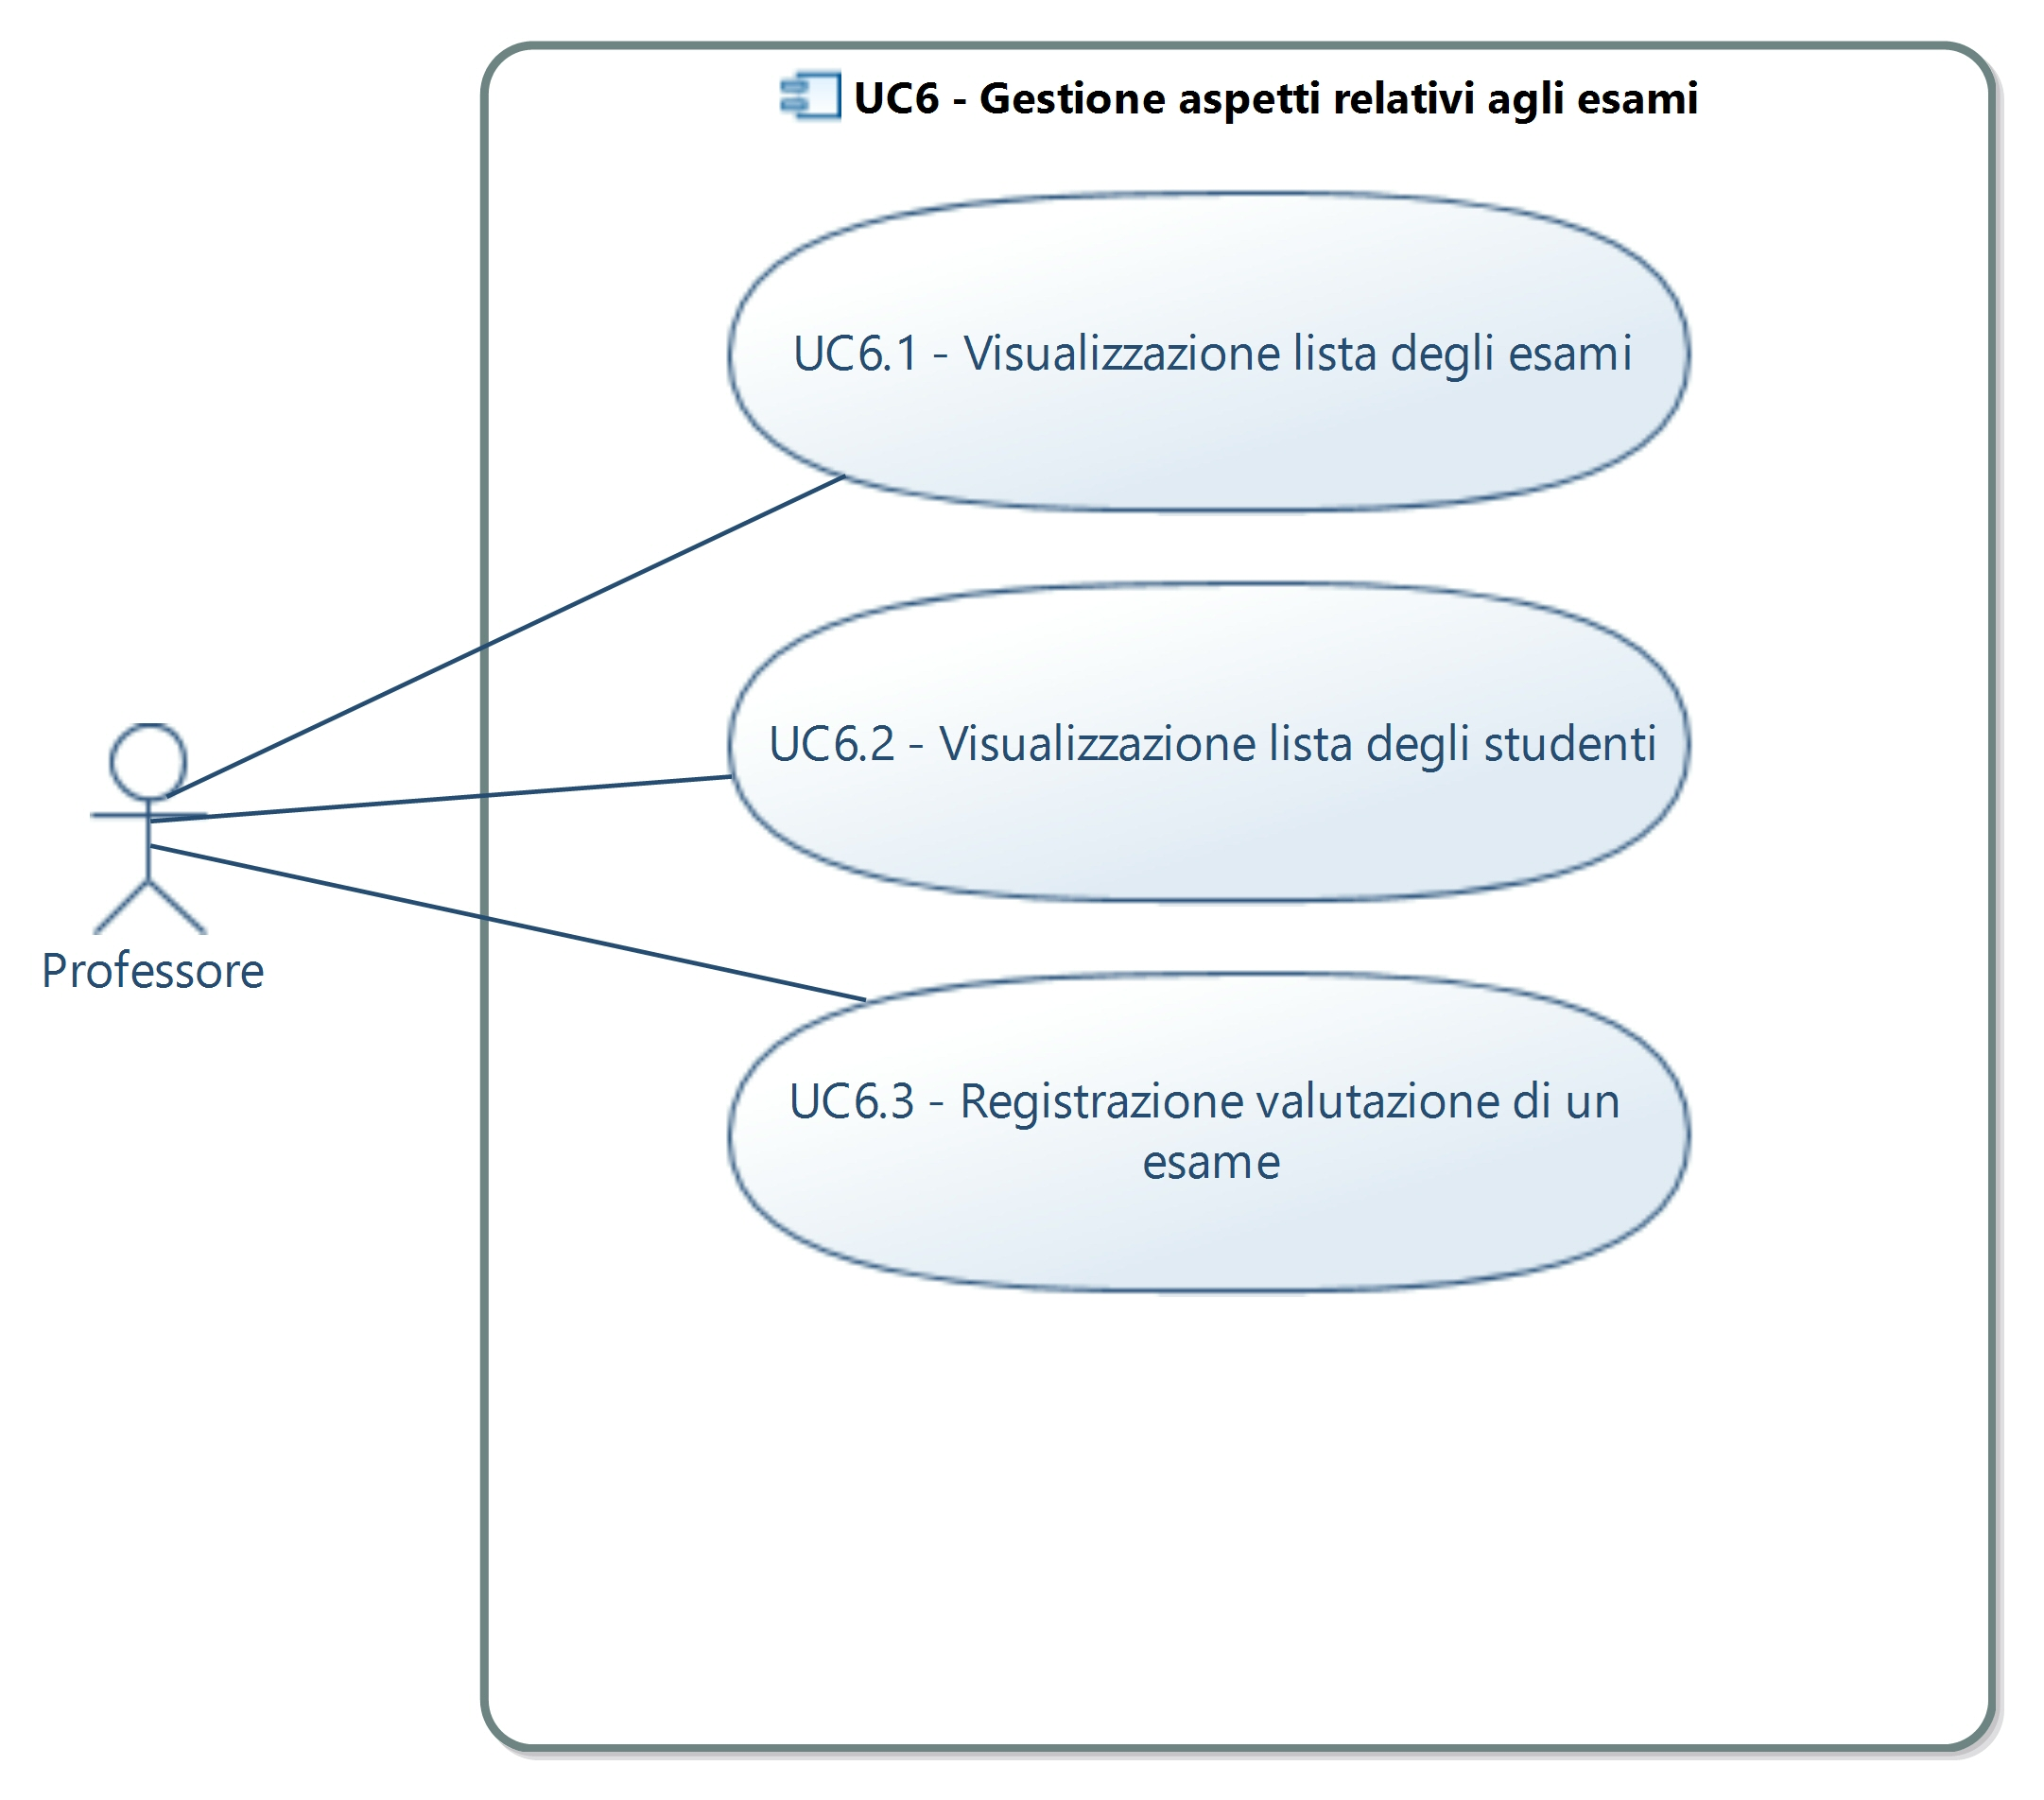
\includegraphics[width=0.8\linewidth]{UC6.jpg}
	\caption{UC6 - Gestione Anni Accademici}
	\label{fig:UC6 - Gestione Anni Accademici}
\end{figure}

\subsection{UC6.1 - Aggiunta anno accademico}
\begin{itemize}
	\item \textbf{Attori primari:} università;
	\item \textbf{Scopo e descrizione:} l'utente è già riconosciuto dal sistema come rappresentante dell'università e aggiunge un \citGloss{anno accademico};
	\item \textbf{Scenario principale:} l'utente che rappresenta l'università inserisce un nuovo anno accademico nel sistema;
	\item \textbf{Precondizione:} il sistema riconosce l'utente nel ruolo di gestore dell'università; 
	\item \textbf{Postcondizione:} all'interno del sistema viene aggiunto un nuovo \citGloss{anno accademico} da parte dell'utente che rappresenta l'università.
\end{itemize}

\begin{figure}[H]
	\centering
	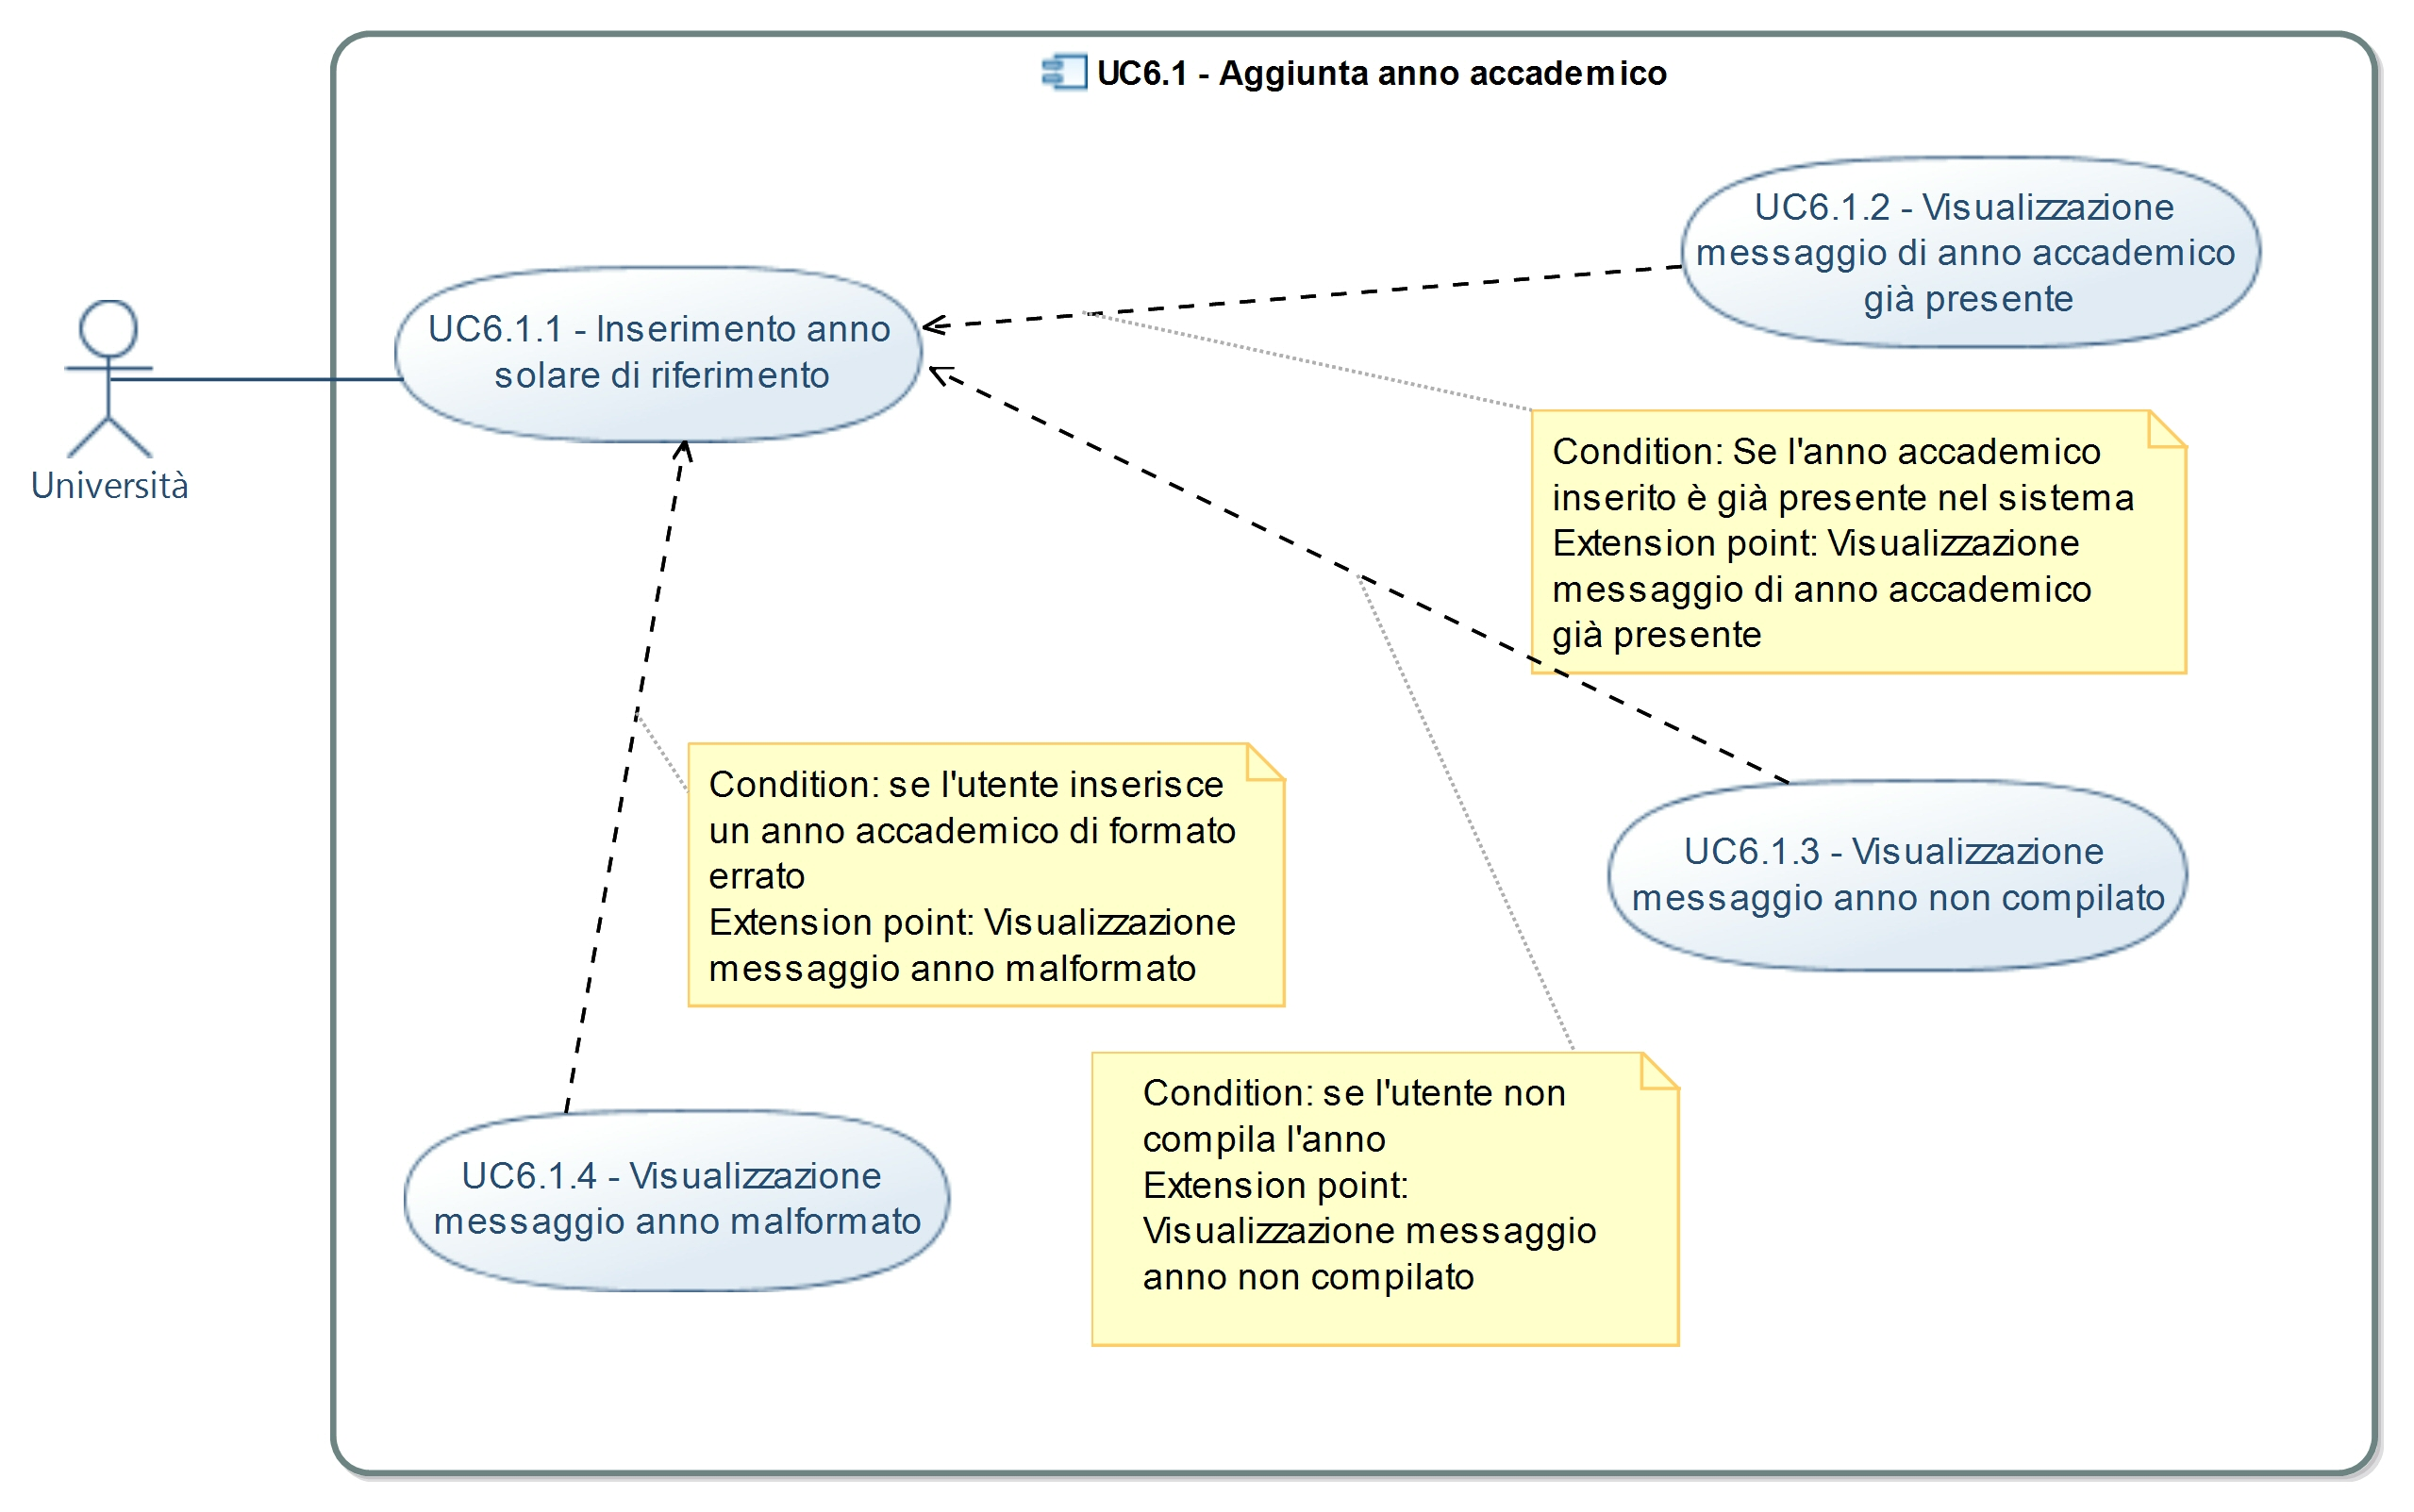
\includegraphics[width=1.1\linewidth]{UC6_1.jpg}
	\caption{UC6.1 - Aggiunta anno accademico}
	\label{fig:UC6.1 - Aggiunta anno accademico}
\end{figure}
\subsection{UC6.1.1 - Inserimento anno solare di riferimento}
	\begin{itemize}
	\item \textbf{Attori primari:} università;
	\item \textbf{Scopo e descrizione:} l'utente è già riconosciuto dal sistema come rappresentante dell'università e inserisce l'anno solare di riferimento per l'inserimento di un anno accademico;
	\item \textbf{Scenario principale:} l'utente che rappresenta l'università inserisce il numero dell'anno solare da aggiungere in un campo fornito dal sistema;
	\item \textbf{Estensioni:}
	\begin{enumerate}
		\item Se l'utente che rappresenta l'università inserisce un anno non numerico viene mostrato un messaggio d'errore relativo all'invalidità del dato fornito [UC6.1.2];
		\item Se l'utente che rappresenta l'università inserisce un'anno già presente nel sistema viene mostrato un messaggio d'errore relativo alla non univocità dell'anno [UC6.1.3];
		\item Se l'utente che rappresenta l'università lascia il campo vuoto l'utente viene avvisato con un relativo messaggio d'errore [UC6.1.4].
	\end{enumerate}
	\item \textbf{Precondizione:} il sistema riconosce l'utente nel ruolo di gestore dell'università, al quale viene fornito un campo di testo per permettere l'inserimento dell'anno solare di riferimento; 
	\item \textbf{Postcondizione:} all'interno del sistema viene aggiunto un nuovo \citGloss{anno accademico} da parte dell'utente che rappresenta l'università con l'anno solare di riferimento indicato.
\end{itemize}
\subsection{UC6.1.2 - Visualizzazione messaggio di anno accademico già presente}
\begin{itemize}
	\item \textbf{Attori primari:} università;
	\item \textbf{Scopo e descrizione:} l'utente che rappresenta l'università visualizza un messaggio che indica che un \citGloss{anno accademico} come quello inserito è già presente nel sistema;
	\item \textbf{Scenario principale:} il sistema mostra all'utente che rappresenta l'università un messaggio d'errore relativo alla non univocità dell'\citGloss{anno accademico} inserito;
	\item \textbf{Precondizione:} il sistema riceve una richiesta di creazione di un nuovo anno accademico da parte dell'utente che gestisce l'università con indicato un anno già presente;
	\item \textbf{Postcondizione:} il sistema avvisa l'utente che non è possibile inserire un anno già presente.
\end{itemize}
\subsection{UC6.1.3 - Visualizzazione messaggio anno non compilato}
\begin{itemize}
	\item \textbf{Attori primari:} università;
	\item \textbf{Scopo e descrizione:} l'utente che rappresenta l'università visualizza un messaggio che lo avvisa di aver lasciato vuoto il campo dell'\citGloss{anno accademico};
	\item \textbf{Scenario principale:} il sistema mostra un messaggio d'errore relativo alla non compilazione dell'\citGloss{anno accademico};
	\item \textbf{Precondizione:} il sistema riceve una richiesta di creazione di un nuovo anno accademico da parte dell'utente che gestisce l'università con l'indicazione dell'anno solare lasciata da compilare; 
	\item \textbf{Postcondizione:} il sistema avvisa l'utente che non è possibile inserire un anno accademico senza indicarne l'anno solare.
\end{itemize}
\subsection{UC6.1.4 - Visualizzazione messaggio anno malformato}
\begin{itemize}
	\item \textbf{Attori primari:} università;
	\item \textbf{Scopo e descrizione:} l'utente che rappresenta l'università visualizza un messaggio che lo informa che l'anno inserito non è numerico;
	\item \textbf{Scenario principale:} il sistema mostra all'utente che rappresenta l'università un messaggio d'errore relativo alla malformazione dell'anno inserito;
	\item \textbf{Precondizione:} il sistema riceve una richiesta di creazione di un nuovo anno accademico da parte dell'utente che gestisce l'università con indicato un anno non numerico; 
	\item \textbf{Postcondizione:} il sistema avvisa l'utente che non è possibile inserire un anno non numerico.
\end{itemize}

\subsection{UC6.2 - Visualizzazione lista di tutti gli anni accademici}
\begin{itemize}
	\item \textbf{Attori primari:} università;
	\item \textbf{Scopo e descrizione:} l'utente è già riconosciuto dal sistema come rappresentante dell'università e visualizza una lista di tutti gli anni accademici presenti nel sistema, visualizzandone l'anno solare di riferimento;
	\item \textbf{Scenario principale:} l'utente che rappresenta l'università richiede la lista di tutti gli anni del sistema;
	\item \textbf{Precondizione:} il sistema riconosce l'utente nel ruolo di gestore dell'università;
	\item \textbf{Postcondizione:} il sistema offre all'utente che gestisce l'università la lista degli anni accademici.
\end{itemize}
\begin{figure}[H]
	\centering
	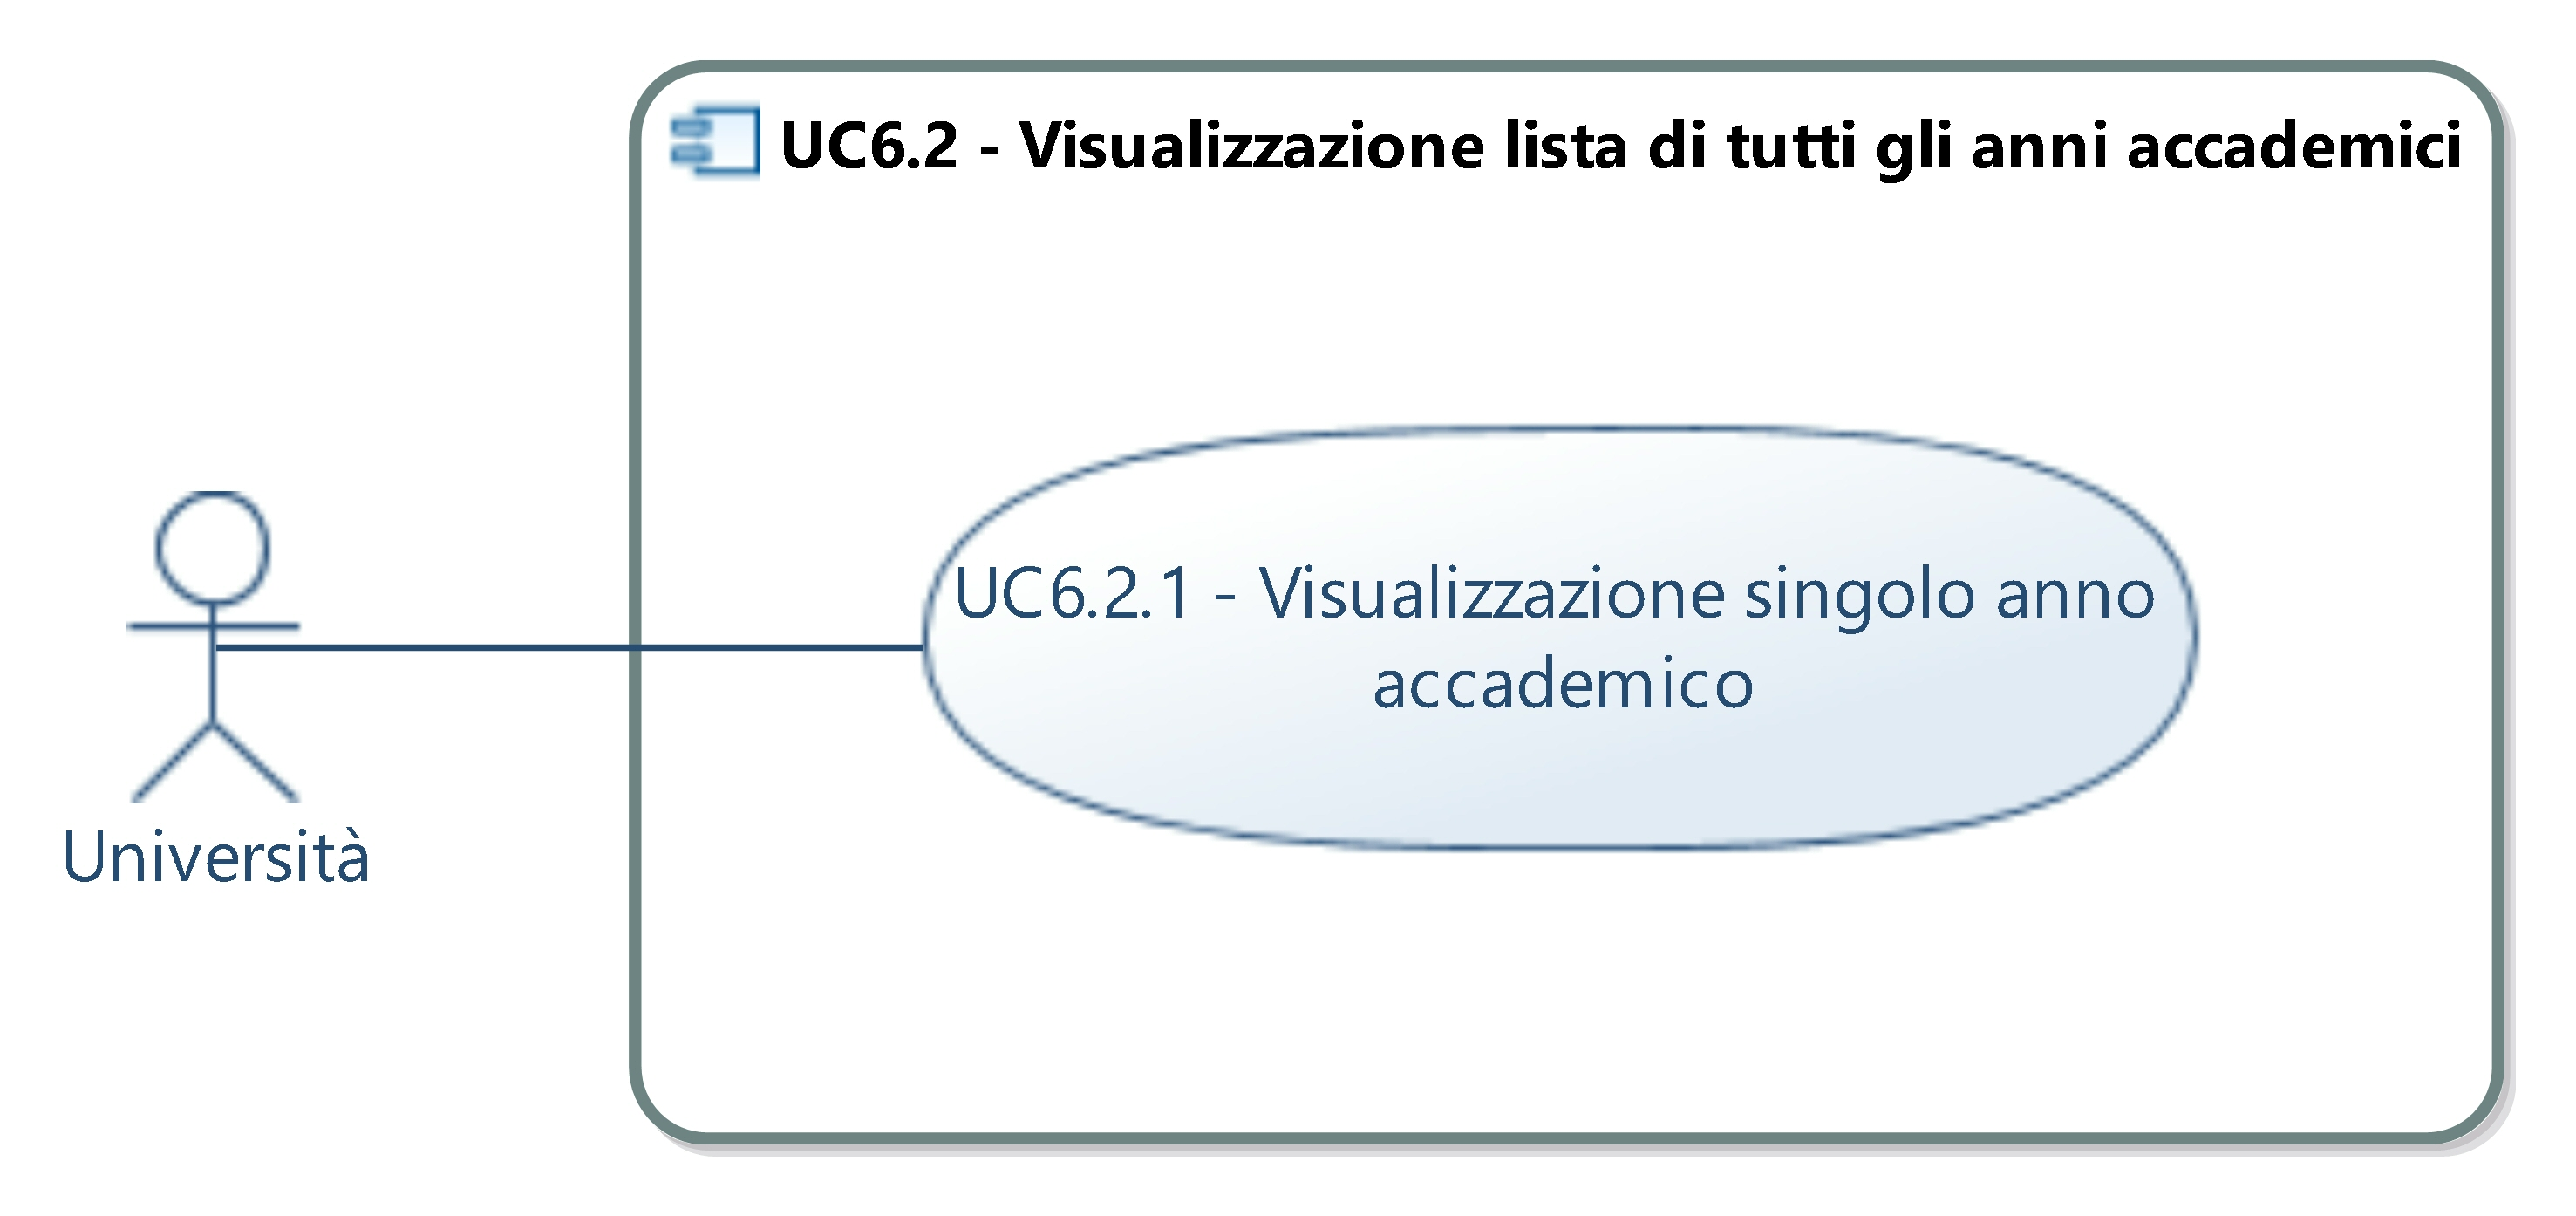
\includegraphics[width=0.7\linewidth]{UC6_2.jpg}
	\caption{UC6.2 - Visualizzazione lista di tutti gli anni accademici}
	\label{fig:UC6.2 - Visualizzazione lista di tutti gli anni accademici}
\end{figure}
\subsection{UC6.2.1 - Visualizzazione anni solari relativi agli anni accademici}
\begin{itemize}
	\item \textbf{Attori primari:} università;
	\item \textbf{Scopo e descrizione:} l'utente già riconosciuto dal sistema come rappresentante dell'università visualizza una lista di tutti gli anni solari relativi agli anni accademici inseriti nella rete \citGloss{Ethereum};
	\item \textbf{Scenario principale:} L'utente che rappresenta l'università richiede al sistema la lista di anni accademici inseriti nel sistema per visualizzarli ed eventualmente compiere operazioni su di esse;
	\item \textbf{Precondizione:} il sistema riconosce l'utente nel ruolo di gestore dell'università e riceve una richiesta di visualizzazione di tutti gli anni accademici;
	\item \textbf{Postcondizione:} il sistema offre all'utente che gestisce l'università la lista degli anni solari relativi agli anni accademici.
\end{itemize}

\subsection{UC6.3 - Eliminazione anno accademico vuoto}
\begin{itemize}
	\item \textbf{Attori primari:} università;
	\item \textbf{Scopo e descrizione:} l'utente che rappresenta l'università desidera la rimozione di un anno accademico che non presenta ancora dei corsi di laurea al suo interno, ad esempio per rimediare a un inserimento con informazioni errate;
	\item \textbf{Scenario principale:} l'utente che rappresenta l'università desidera rimuovere un anno accademico che non presenta corsi collegati dal sistema;
	\item \textbf{Precondizione:} il sistema fornisce una lista degli \citGloss{anni accademici} [UC6.2] all'utente;
	\item \textbf{Postcondizione:} L'\citGloss{anno accademico} che l'utente desidera cancellare viene rimosso dal sistema.
\end{itemize}

\subsection{UC7 - Gestione corsi di laurea}
\begin{itemize}
	\item \textbf{Attori primari:} amministratore;
	\item \textbf{Scopo e descrizione:} l'amministratore è in grado di eseguire operazioni sui corsi di laurea. La gestione non è stata assegnata al gestore dell'università in quanto molto onerosa in termini di tempo e quindi difficilmente adempibile da una singola persona;
	\item \textbf{Scenario principale:} l'amministratore visualizza una lista di operazioni eseguibili sui corsi di laurea e ne sceglie una;
	\item \textbf{Precondizione:} il sistema riconosce l'utente come amministratore e fornisce la lista delle funzionalità alle quali ha accesso relative all'amministrazione dei corsi di laurea;
	\item \textbf{Postcondizione:} il sistema effettua le operazioni richieste riguardanti la gestione dei corsi di laurea.
\end{itemize}

\begin{figure}[H]
	\centering
	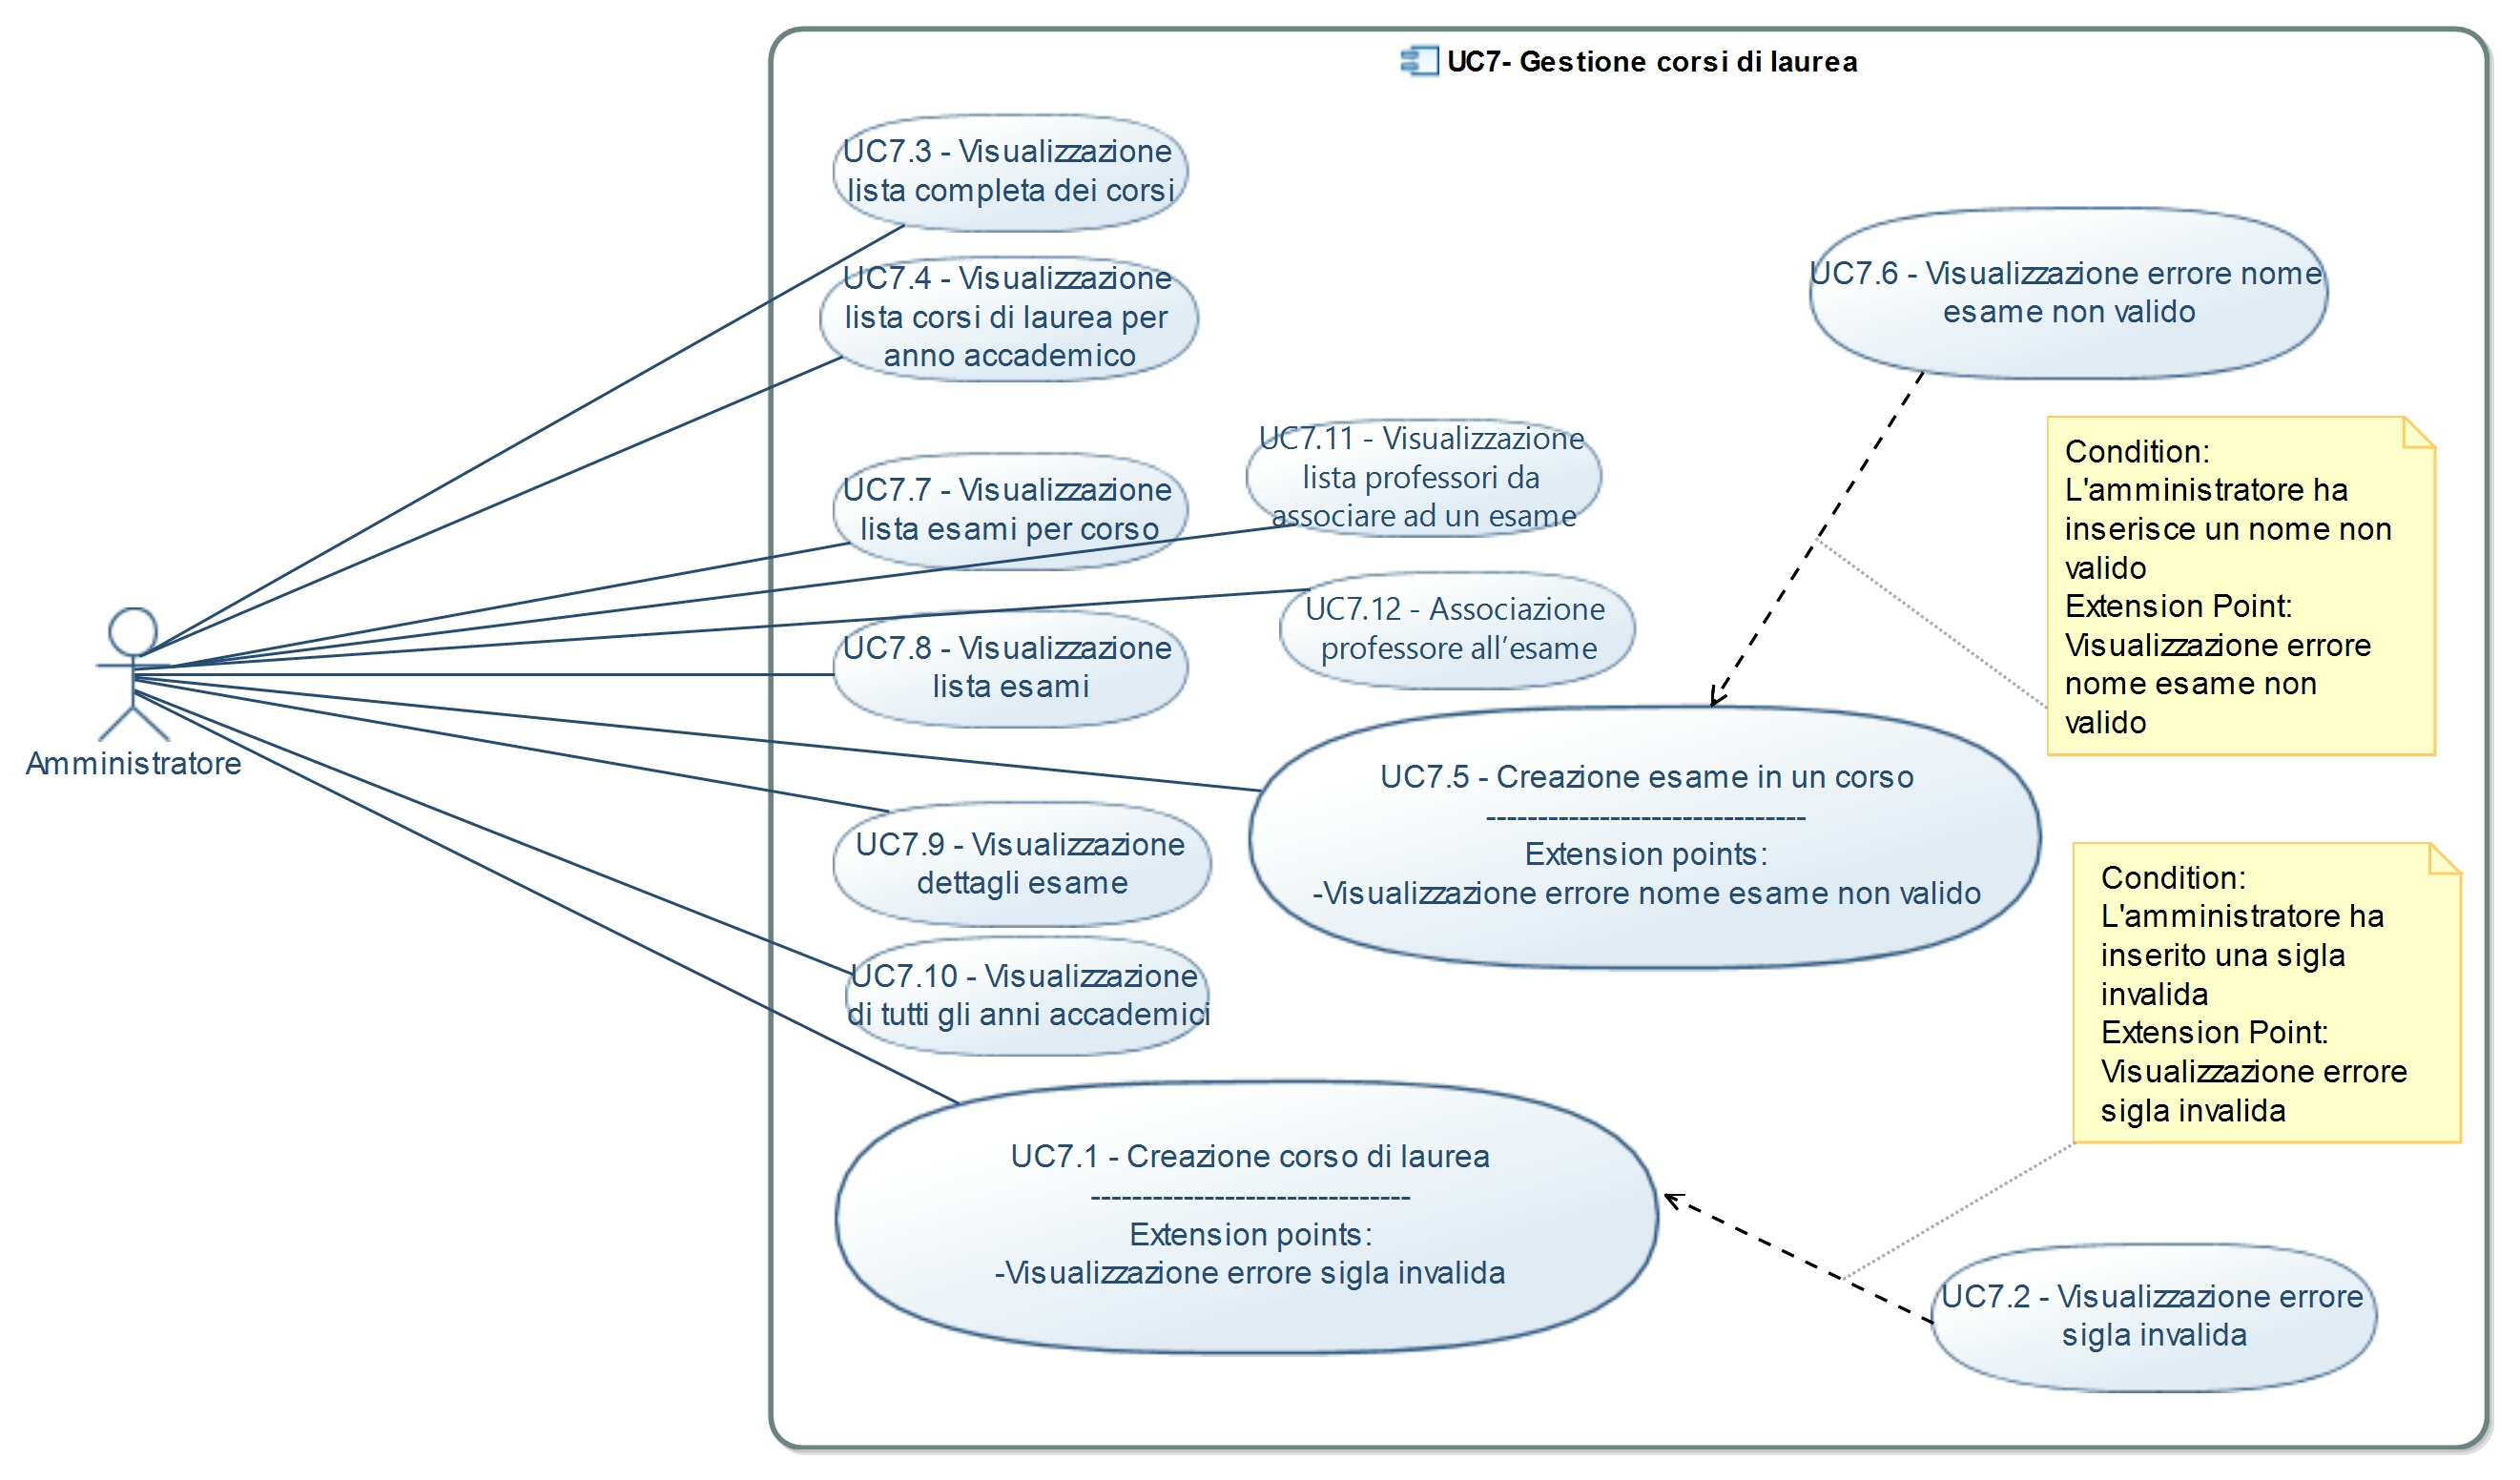
\includegraphics[width=1.1\linewidth]{UC7.jpg}
	\caption{UC7 - Gestione Corsi di laurea}
	\label{fig:UC7 - Gestione Corsi di laurea}
\end{figure}

\subsection{UC7.1 - Creazione corso di laurea}
\begin{itemize}
	\item \textbf{Attori primari:} amministratore;
	\item \textbf{Scopo e descrizione:} l'amministratore crea un nuovo corso di laurea associato a un \citGloss{anno accademico}, indicando la sigla da utilizzare per riferirsi al corso;
	\item \textbf{Scenario principale:} l'amministratore inserisce un nuovo corso di laurea;
	\item \textbf{Precondizione:} il sistema identifica l'utente come amministratore e fornisce una lista di \citGloss{anni accademici} [UC7.8];
	\item \textbf{Postcondizione:} viene creato e inserito nel sistema un nuovo \citGloss{corso di laurea} relativo all'anno accademico indicato dall'utente.
\end{itemize}

\begin{figure}[H]
	\centering
	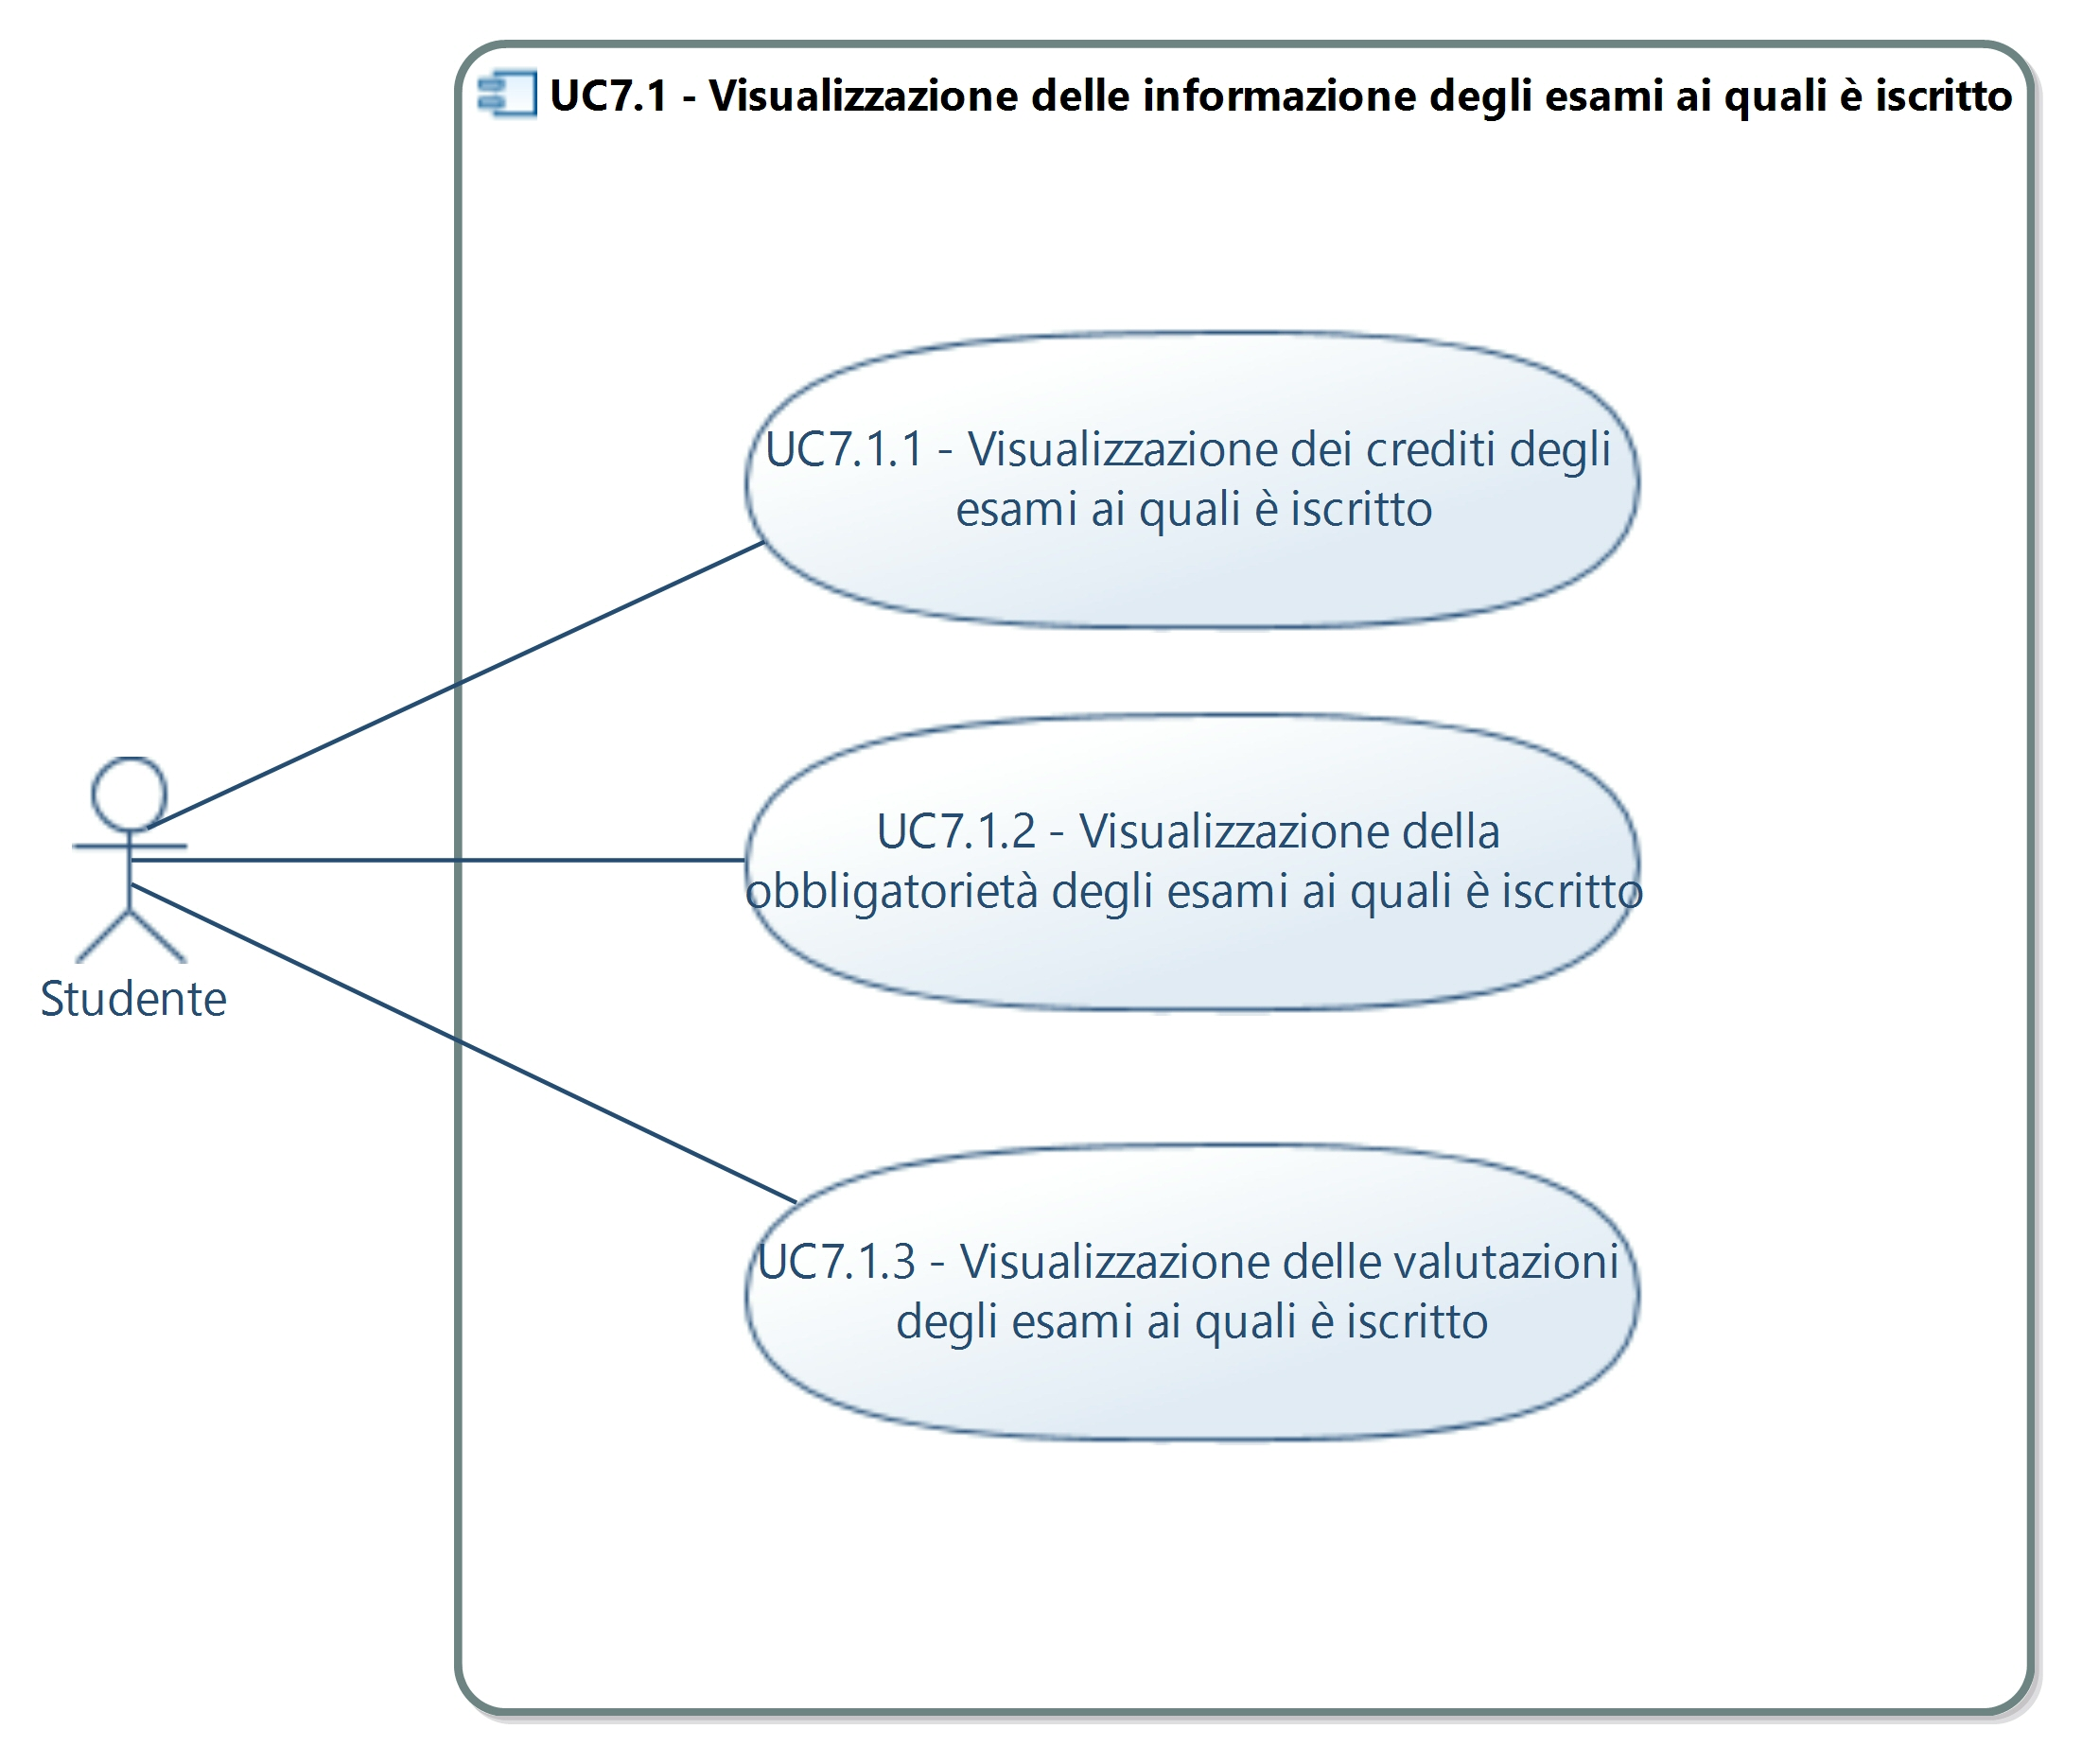
\includegraphics[width=1.1\linewidth]{UC7_1.jpg}
	\caption{UC7.1 - Creazione corso di laurea}
	\label{fig:UC7.1 - Creazione corso di laurea}
\end{figure}

\subsection{UC7.1.1 - Inserimento sigla corso di laurea}
\begin{itemize}
	\item \textbf{Attori primari:} amministratore;
	\item \textbf{Scopo e descrizione:} l'amministratore specifica la sigla del corso di laurea che vuole inserire;
	\item \textbf{Scenario principale:} l'amministratore inserisce la sigla del corso di laurea;
	\item \textbf{Estensioni:}
	\begin{enumerate}
		\item Se l'amministratore inserisce una sigla invalida viene avvisato con un messaggio [UC7.1.2].
	\end{enumerate}
	\item \textbf{Precondizione:} il sistema offre all'amministratore un campo dati per inserire la sigla; 
	\item \textbf{Postcondizione:} il sistema riceve la sigla del corso di laurea.
\end{itemize}

\subsection{UC7.1.2 - Visualizzazione errore sigla invalida}
\begin{itemize}
	\item \textbf{Attori primari:} amministratore;
	\item \textbf{Scopo e descrizione:} viene mostrato un messaggio d'errore per avvisare l'amministratore che non è possibile utilizzare la sigla inserita, in quanto non rispetta il pattern indicato dal sistema oppure risulta già in uso;
	\item \textbf{Scenario principale:} il sistema avvisa l'amministratore che non è possibile utilizzare la sigla indicata;
	\item \textbf{Precondizione:} il sistema riceve una richiesta di creazione di un \citGloss{corso di laurea} utilizzando una sigla che non rispetta i \citGloss{requisiti} indicati dal sistema; 
	\item \textbf{Postcondizione:} il sistema avvisa l'amministratore dell'impossibilità di utilizzare quella determinata sigla per la creazione di un nuovo corso, indicandogli la forma corretta.
\end{itemize}

\subsection{UC7.2 - Visualizzazione lista completa dei corsi}
\begin{itemize}
	\item \textbf{Attori primari:} amministratore;
	\item \textbf{Scopo e descrizione:} vengono mostrati tutti i corsi di laurea presenti nel sistema, visualizzandone la sigla e l'anno solare dell'anno accademico associato;
	\item \textbf{Scenario principale:} l'amministratore visualizza tutti i corsi di laurea presenti nel sistema;
	\item \textbf{Precondizione:} il sistema riconosce l'utente come amministratore e fornisce la lista delle funzionalità alle quali ha accesso relative all'amministrazione dei corsi di laurea; 
	\item \textbf{Postcondizione:} il sistema fornisce all'utente la lista completa dei corsi.
\end{itemize}
\begin{figure}[H]
	\centering
	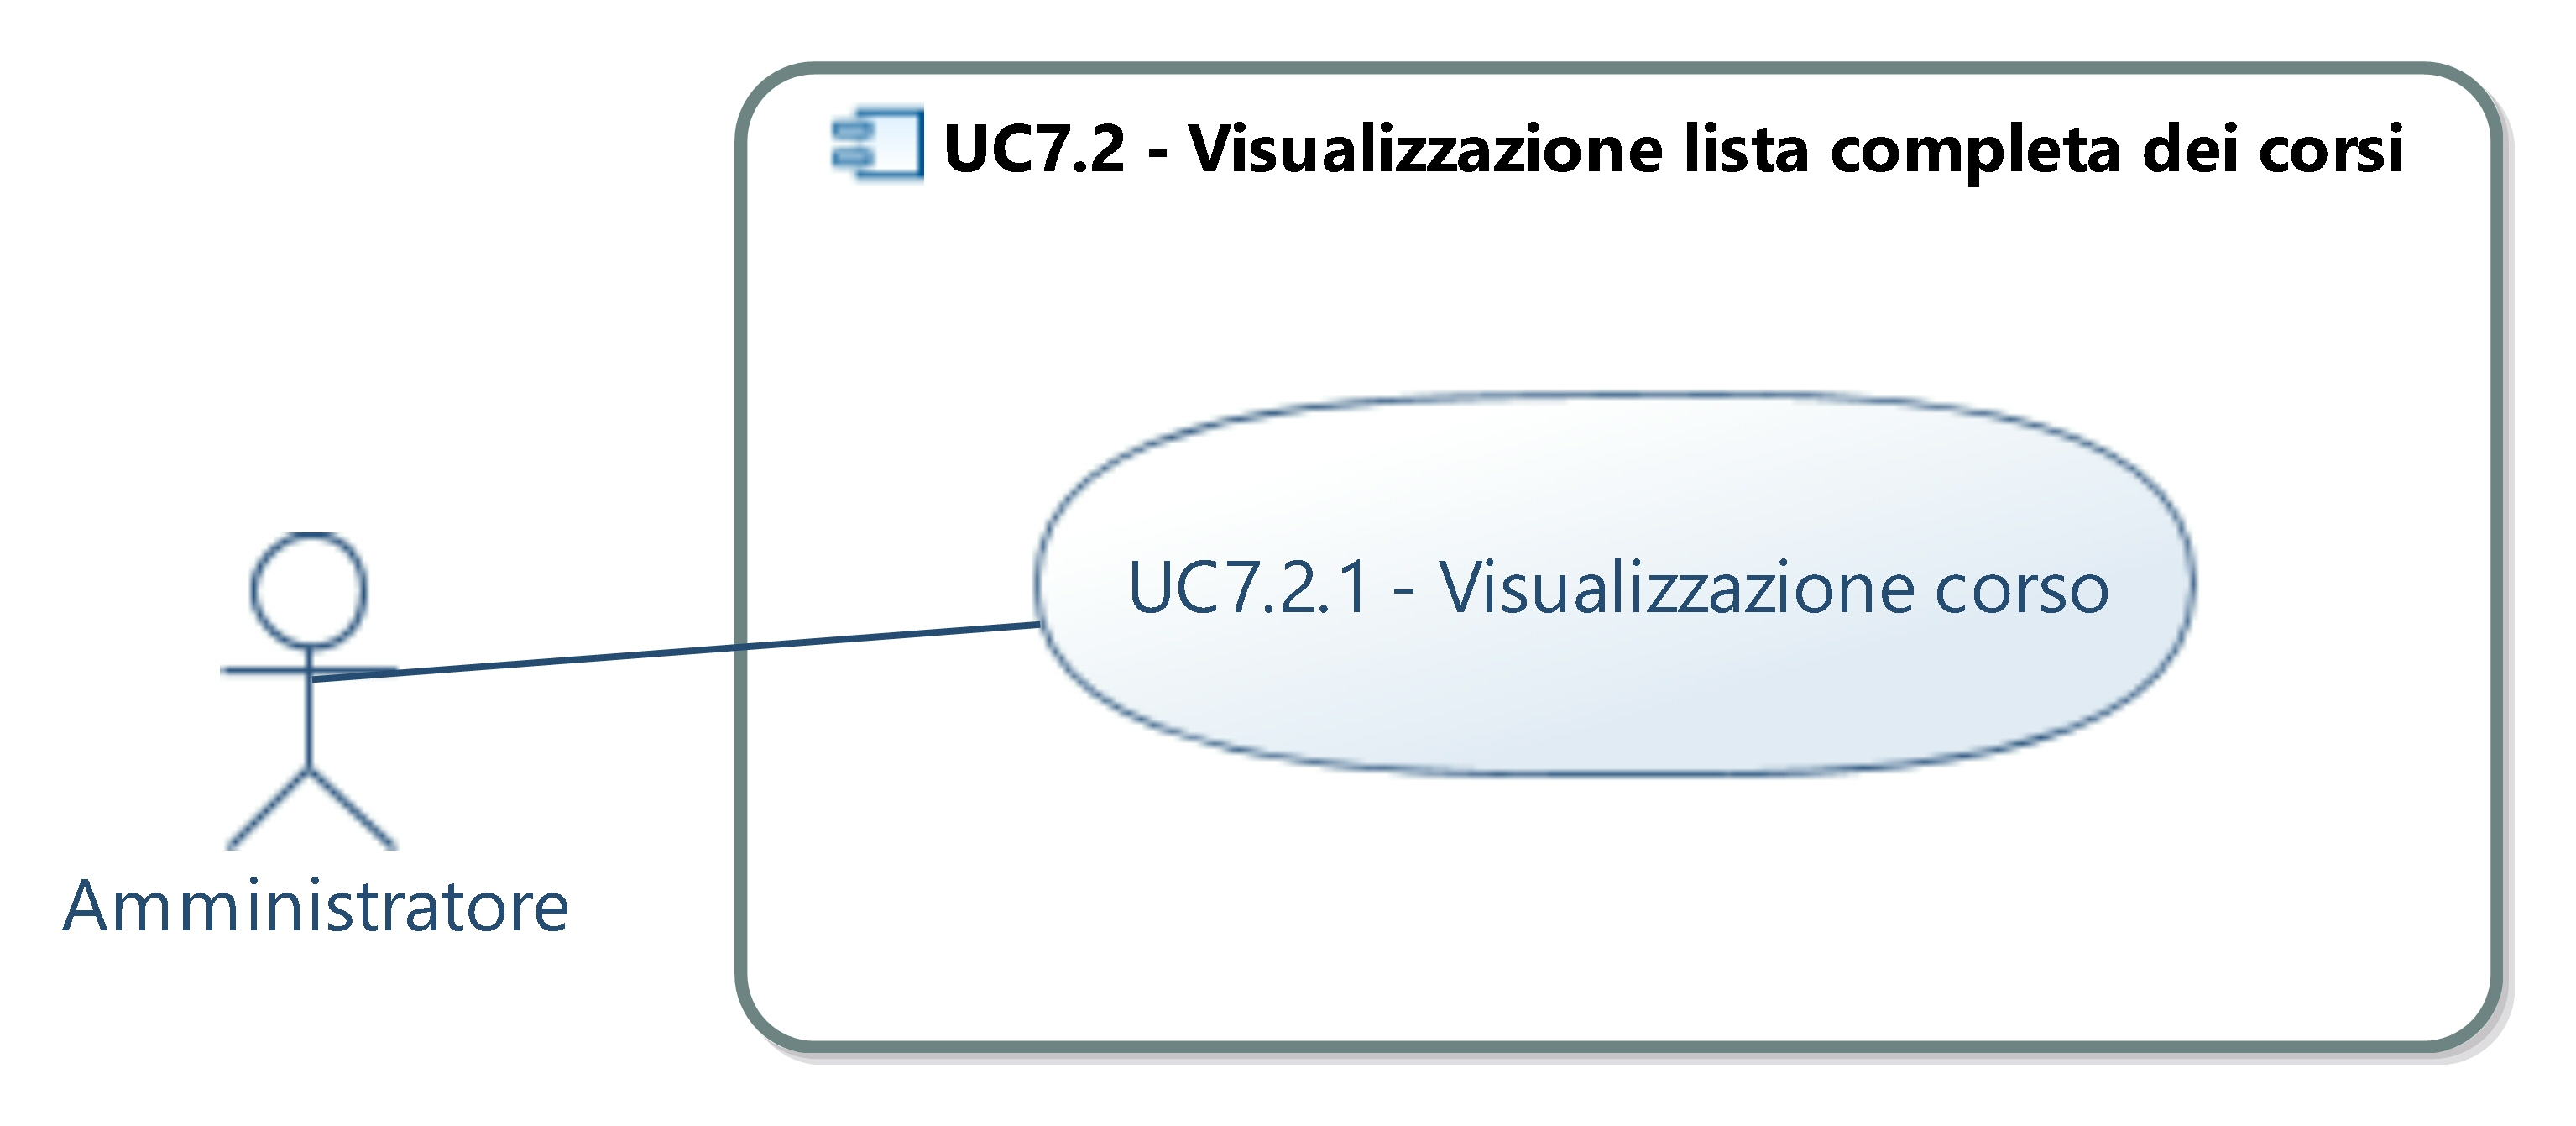
\includegraphics[width=0.8\linewidth]{UC7_2.jpg}
	\caption{UC7.2 - Visualizzazione lista completa dei corsi}
	\label{fig:UC7.2 - Visualizzazione lista completa dei corsi}
\end{figure}
\subsection{UC7.2.1 - Visualizzazione sigle dei corsi di laurea}
\begin{itemize}
	\item \textbf{Attori primari:} amministratore;
	\item \textbf{Scopo e descrizione:} l'amministratore visualizza la lista delle sigle relative ai corsi di laurea presenti nel sistema;
	\item \textbf{Scenario principale:} l'amministratore richiede una lista di corsi di laurea presenti nel sistema;
	\item \textbf{Precondizione:} il sistema riconosce l'utente come amministratore e riceve una richiesta di visualizzazione dei corsi di laurea; 
	\item \textbf{Postcondizione:} il sistema fornisce all'utente la sigla relativa a ogni corso di laurea.
\end{itemize}
\subsection{UC7.2.2 - Visualizzazione anni solari degli anni accademici associati ai corsi di laurea}
\begin{itemize}
	\item \textbf{Attori primari:} amministratore;
	\item \textbf{Scopo e descrizione:} l'amministratore visualizza la lista degli anni solari degli anni accademici relativi ai corsi di laurea presenti nel sistema;
	\item \textbf{Scenario principale:} l'amministratore richiede una lista di corsi di laurea presenti nel sistema;
	\item \textbf{Precondizione:} il sistema riconosce l'utente come amministratore e riceve una richiesta di visualizzazione dei corsi di laurea; 
	\item \textbf{Postcondizione:} il sistema fornisce all'utente l'anno solare dell'anno accademico relativo a ogni corso di laurea.
\end{itemize}
\subsection{UC7.3 - Visualizzazione lista corsi di laurea per anno accademico}
\begin{itemize}
	\item \textbf{Attori primari:} amministratore;
	\item \textbf{Scopo e descrizione:} vengono visualizzati i corsi di laurea relativi a un determinato \citGloss{anno accademico}, ottenendone le sigle;
	\item \textbf{Precondizione:} il sistema riconosce l'utente come amministratore e fornisce una lista di anni accademici [UC7.8];
	\item \textbf{Postcondizione:} il sistema fornisce all'utente la lista dei corsi di laurea relativi all'anno accademico indicato dall'utente.
\end{itemize}
\begin{figure}[H]
	\centering
	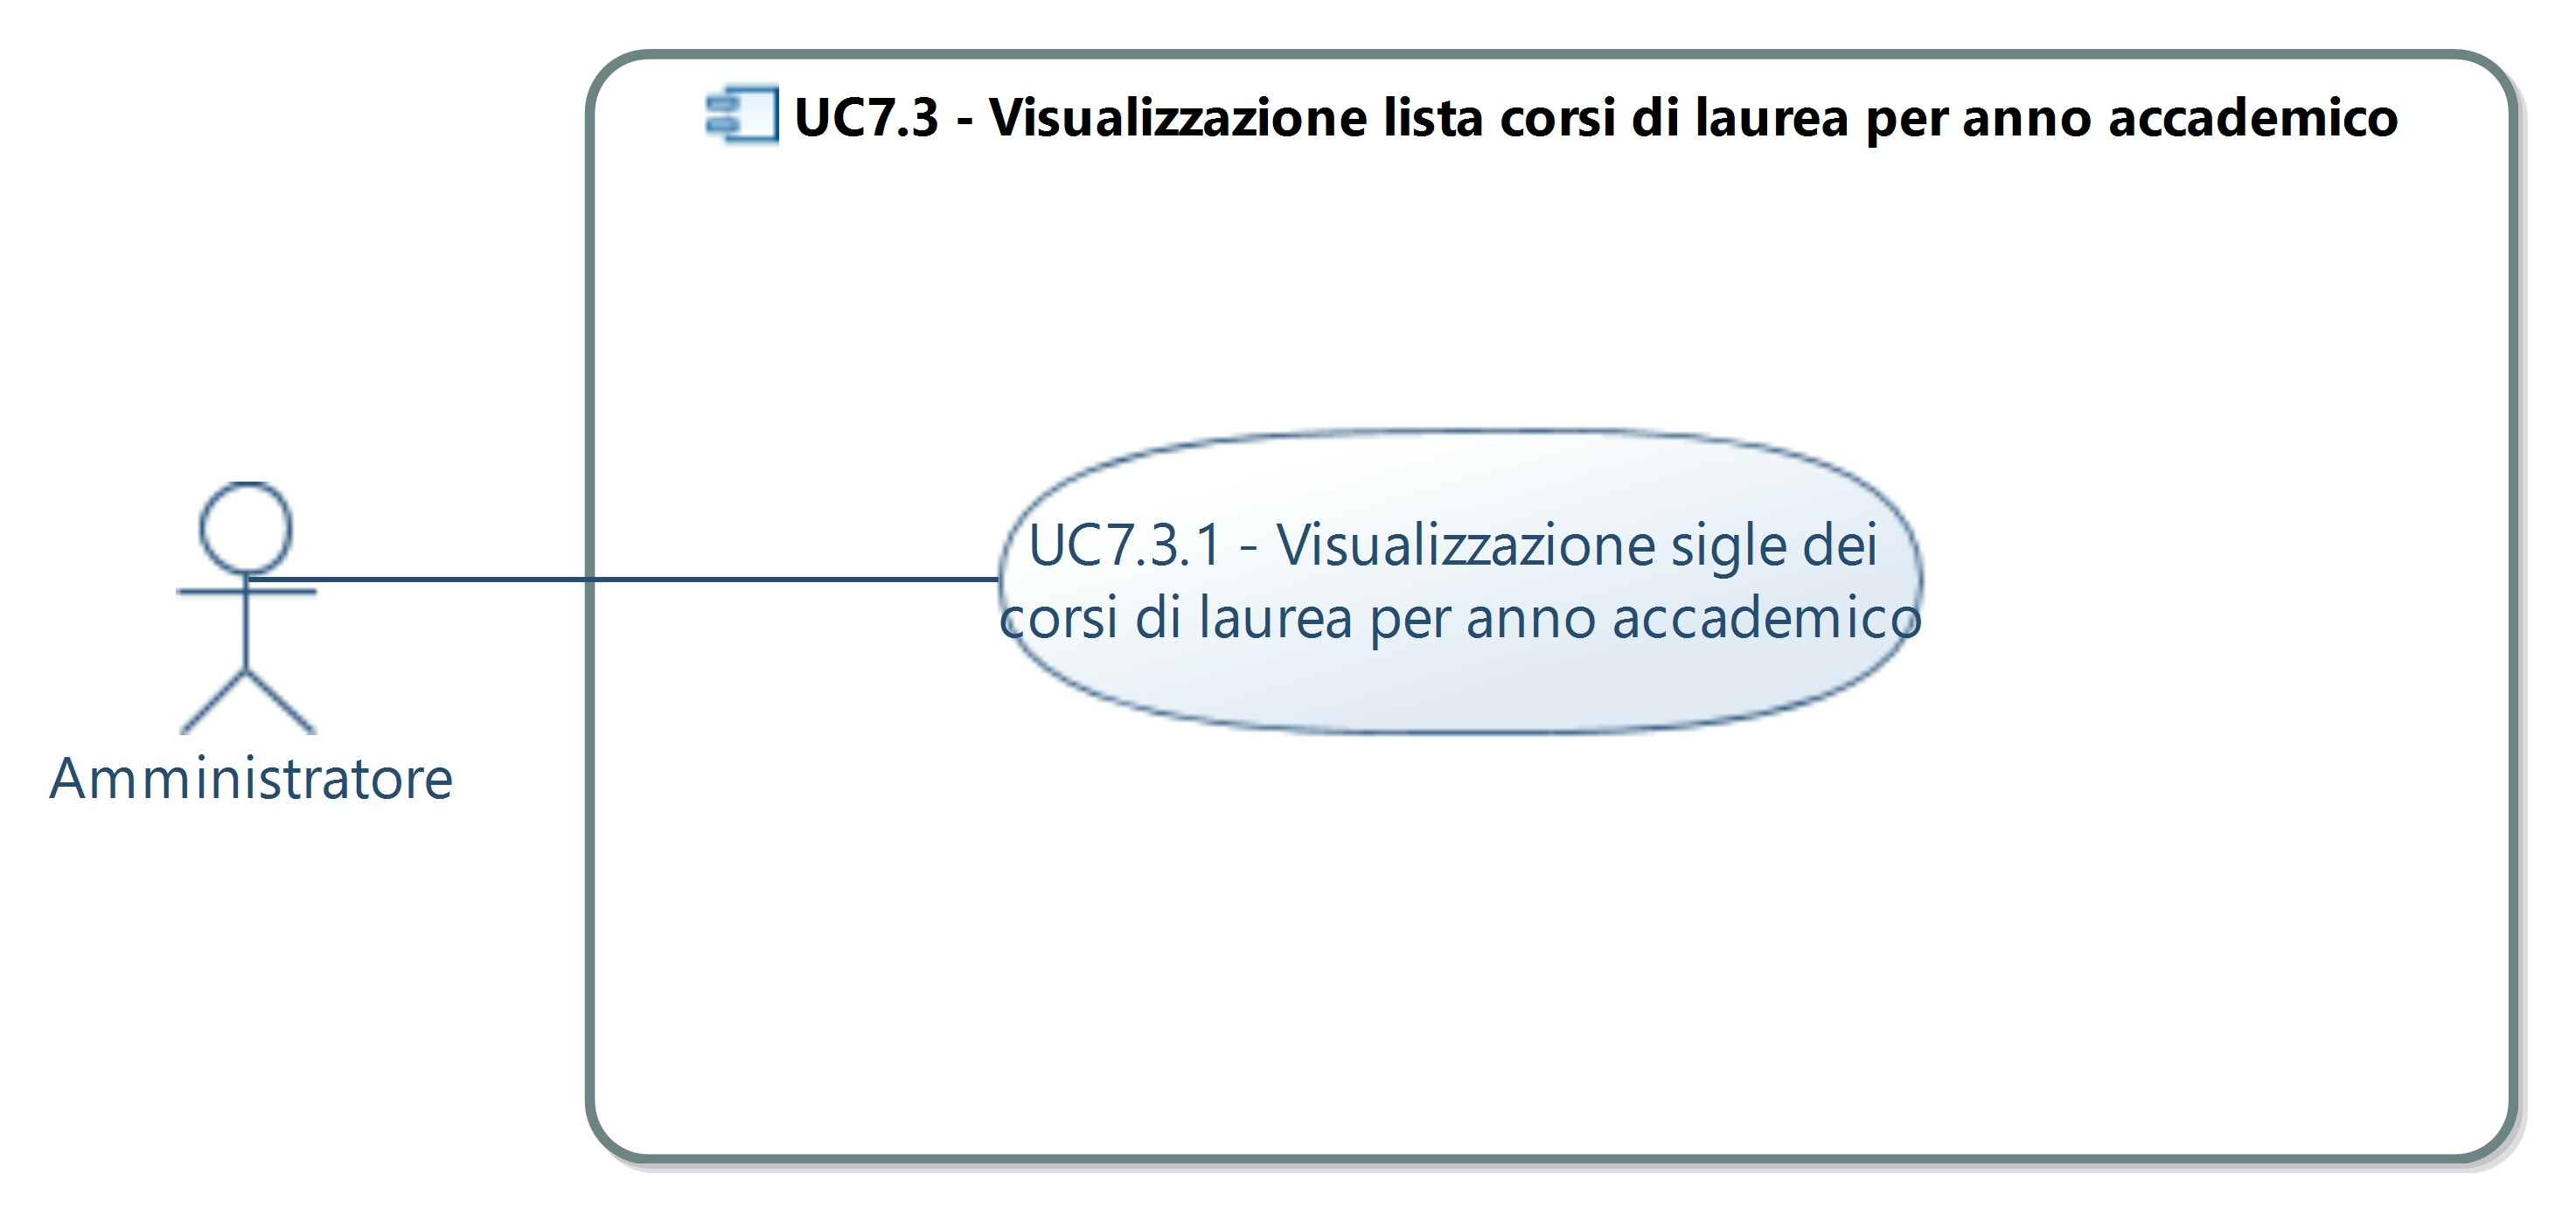
\includegraphics[width=0.7\linewidth]{UC7_3.jpg}
	\caption{UC7.3 - Visualizzazione lista corsi di laurea per anno accademico}
	\label{fig:UC7.3 - Visualizzazione lista corsi di laurea per anno accademico}
\end{figure}
\subsection{UC7.3.1 - Visualizzazione sigle dei corsi di laurea per anno accademico}
\begin{itemize}
	\item \textbf{Attori primari:} amministratore;
	\item \textbf{Scopo e descrizione:} l'amministratore visualizza la lista delle sigle relative ai corsi di laurea presenti nel sistema associati a un determinato anno accademico;
	\item \textbf{Scenario principale:} l'amministratore richiede una lista di corsi di laurea associati a un determinato anno accademico presenti nel sistema;
	\item \textbf{Precondizione:} il sistema riconosce l'utente come amministratore e riceve una richiesta di visualizzazione dei corsi di laurea relativi a un determinato anno accademico; 
	\item \textbf{Postcondizione:} il sistema fornisce all'utente la sigla relativa a ogni corso di laurea dell'anno accademico indicatogli.
\end{itemize}

\subsection{UC7.4 - Creazione esame in un corso}
\begin{itemize}
	\item \textbf{Attori primari:} amministratore;
	\item \textbf{Scopo e descrizione:} l'amministratore crea e assegna un esame all'interno di un \citGloss{corso di laurea} indicandone il nome, la quantità di crediti e l'obbligatorietà;
	\item \textbf{Scenario principale:} l'amministratore inserisce un nuovo esame all'interno di un corso;
	\item \textbf{Precondizione:} il sistema riconosce l'utente come amministratore e fornisce una lista di corsi di laurea per \citGloss{anno accademico} [UC7.2];
	\item \textbf{Postcondizione:} all'interno del sistema viene creato un nuovo esame associato al \citGloss{corso di laurea} indicato dall'utente.
\end{itemize}
\begin{figure}[H]
	\centering
	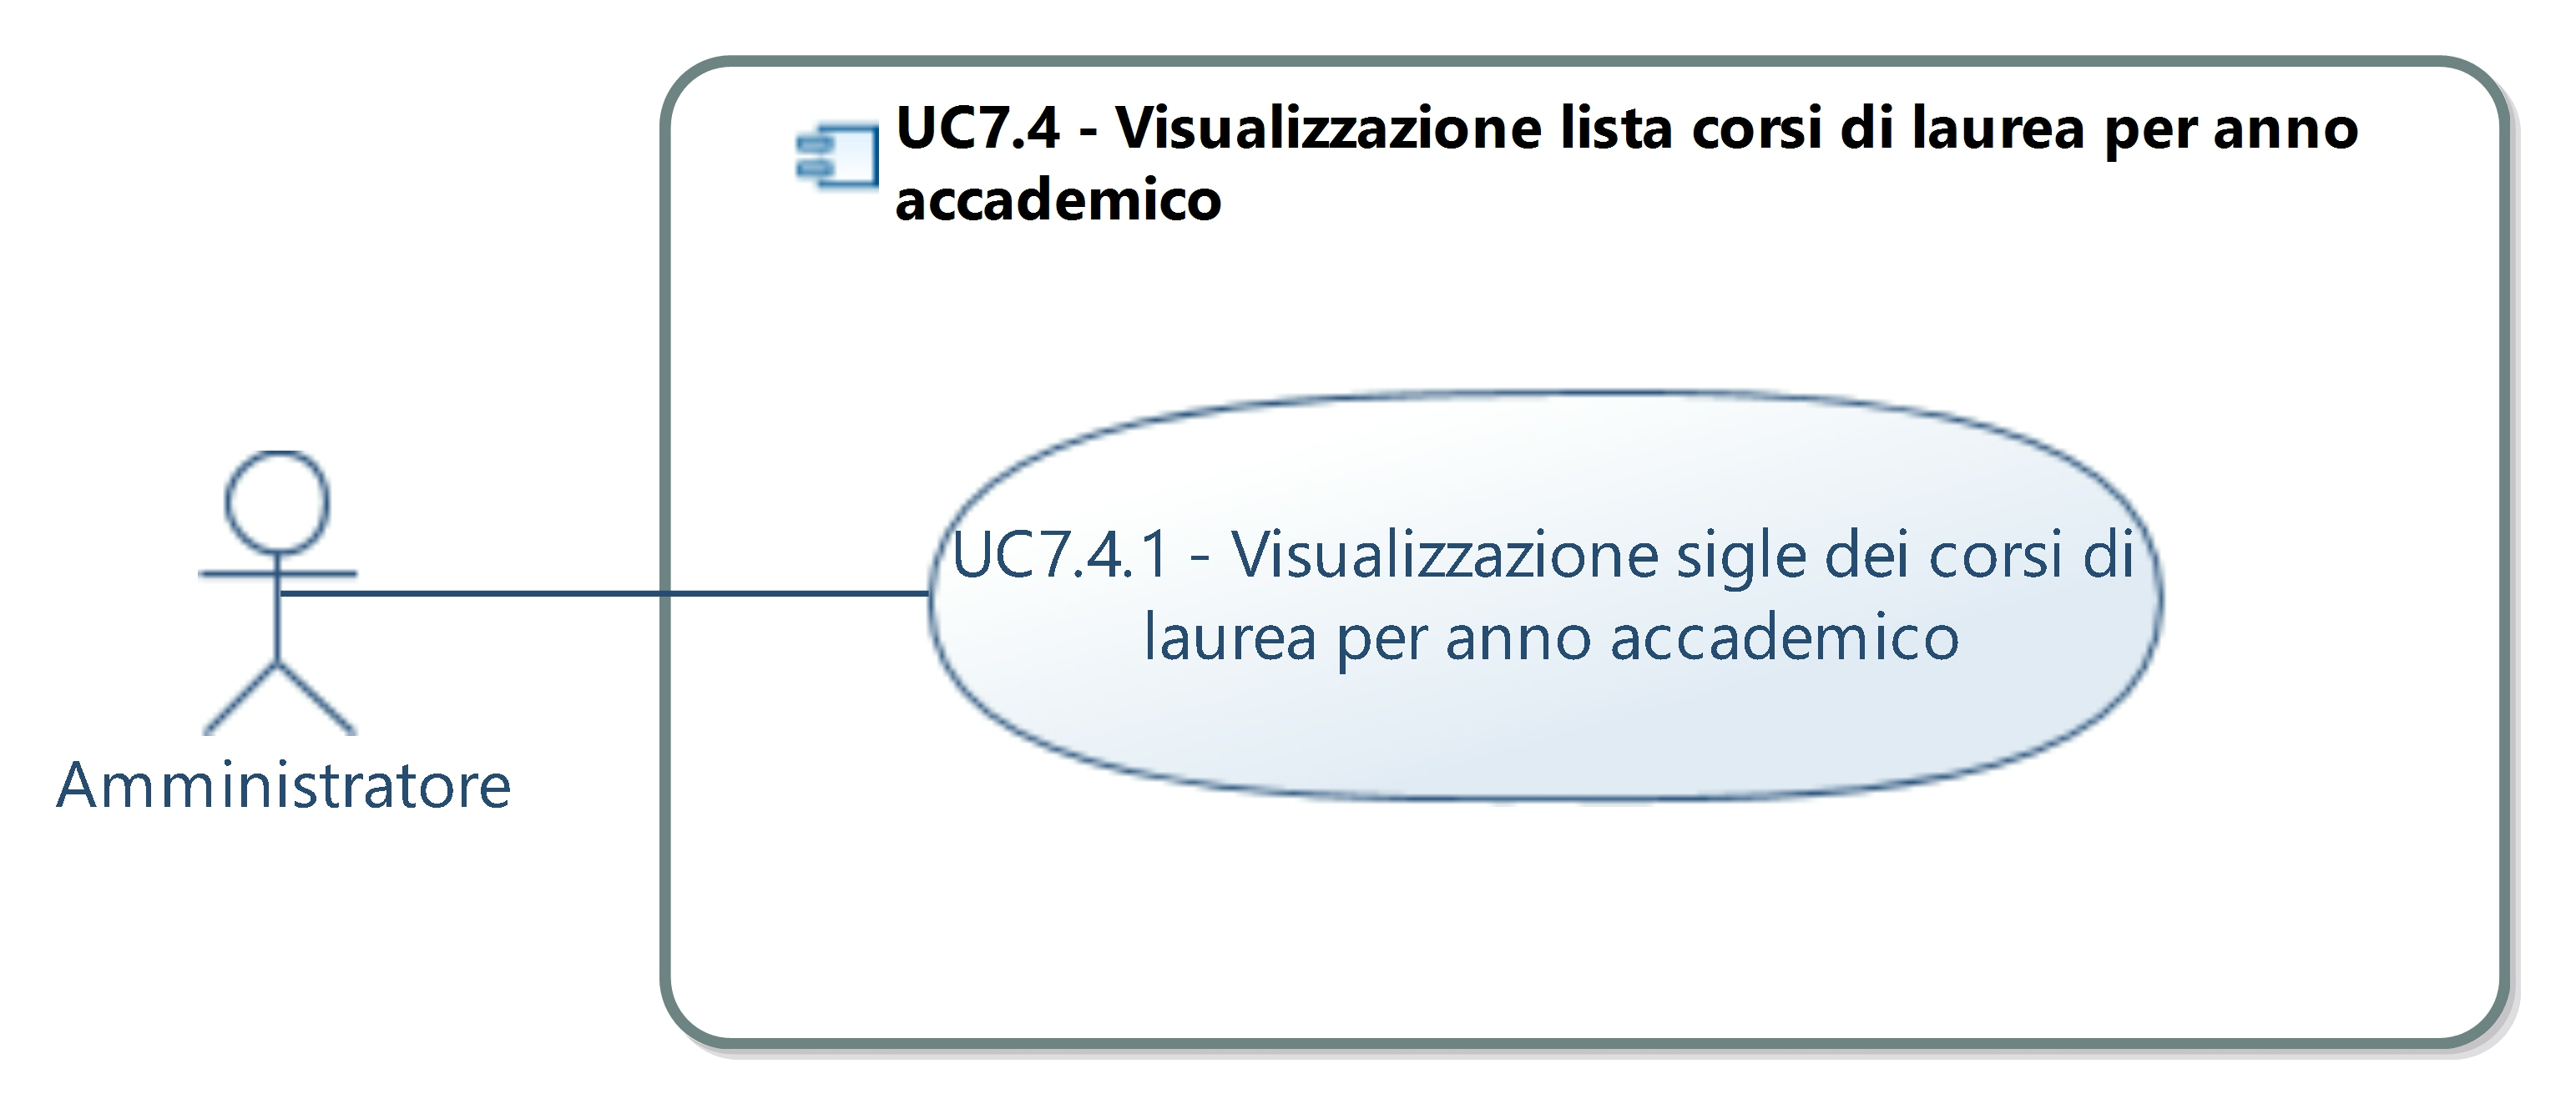
\includegraphics[width=1.0\linewidth]{UC7_4.jpg}
	\caption{UC7.4 - Creazione esame in un corso}
	\label{fig:UC7.4 - Creazione esame in un corso}
\end{figure}
\subsection{UC7.4.1 - Inserimento nome esame}
\begin{itemize}
	\item \textbf{Attori primari:} amministratore;
	\item \textbf{Scopo e descrizione:} l'amministratore specifica il nome dell'esame da inserire nel corso;
	\item \textbf{Scenario principale:} l'amministratore inserisce il nome dell'esame;
	\item \textbf{Estensioni:}
	\begin{enumerate}
		\item Se il nome non rispetta i vincoli indicati dal sistema l'amministratore viene avvisato con un messaggio d'errore [UC7.4.4].
	\end{enumerate}
	\item \textbf{Precondizione:} il sistema offre all'amministratore un campo da compilare con il nome dell'esame; 
	\item \textbf{Postcondizione:} il sistema riceve il nome dell'esame immesso dall'amministratore.
\end{itemize}
\subsection{UC7.4.2 - Inserimento numero crediti esami}
\begin{itemize}
	\item \textbf{Attori primari:} amministratore;
	\item \textbf{Scopo e descrizione:} l'amministratore specifica il numero di crediti dell'esame da inserire nel corso;
	\item \textbf{Scenario principale:} l'amministratore inserisce il numero di crediti dell'esame;
	\item \textbf{Estensioni:}
	\begin{enumerate}
		\item Se il numero di crediti non rispetta i vincoli indicati dal sistema l'amministratore viene avvisato con un messaggio d'errore [UC7.4.5].
	\end{enumerate}
	\item \textbf{Precondizione:} il sistema offre all'amministratore un campo da compilare con il numero di crediti dell'esame; 
	\item \textbf{Postcondizione:} il sistema riceve il numero di crediti immesso dall'amministratore.
\end{itemize}
\subsection{UC7.4.3 - Inserimento obbligatorietà esame}
\begin{itemize}
	\item \textbf{Attori primari:} amministratore;
	\item \textbf{Scopo e descrizione:} l'amministratore indica se l'esame da inserire nel corso è obbligatorio o meno;
	\item \textbf{Scenario principale:} l'amministratore inserisce l'obbligatorietà dell'esame;
	\item \textbf{Precondizione:} il sistema offre all'amministratore un campo per specificare l'obbligatorietà dell'esame; 
	\item \textbf{Postcondizione:} il sistema riceve la specifica di obbligatorietà immessa dall'amministratore.
\end{itemize}
\subsection{UC7.4.4 - Visualizzazione errore nome esame non valido}
\begin{itemize}
	\item \textbf{Attori primari:} amministratore;
	\item \textbf{Scopo e descrizione:} viene mostrato un messaggio d'errore relativo all'invalidità del nome del corso, in quanto non rispetta un pattern indicato dal sistema oppure già utilizzato;
	\item \textbf{Scenario principale:} l'amministratore visualizza il messaggio d'errore;
	\item \textbf{Precondizione:} il sistema riceve un nome che non rispetta i \citGloss{requisiti} indicati; 
	\item \textbf{Postcondizione:} il sistema indica all'utente che il nome inserito non è valido, indicando quali vincoli deve soddisfare.
\end{itemize}
\subsection{UC7.4.5 - Visualizzazione errore numero crediti esame non valido}
\begin{itemize}
	\item \textbf{Attori primari:} amministratore;
	\item \textbf{Scopo e descrizione:} viene mostrato un messaggio d'errore relativo all'invalidità del numero di crediti del corso, in quanto non rispetta un pattern indicato dal sistema oppure già utilizzato;
	\item \textbf{Scenario principale:} l'amministratore visualizza il messaggio d'errore;
	\item \textbf{Precondizione:} il sistema riceve un numero di crediti che non rispetta i \citGloss{requisiti} indicati; 
	\item \textbf{Postcondizione:} il sistema indica all'utente che il numero di crediti inserito non è valido, indicando quali vincoli deve soddisfare.
\end{itemize}

\subsection{UC7.5 - Visualizzazione lista esami per corso}
\begin{itemize}
	\item \textbf{Attori primari:} amministratore;
	\item \textbf{Scopo e descrizione:} vengono visualizzati gli esami relativi a un determinato \citGloss{corso di laurea}, con indicato per ognuno di essi il nome, il numero di crediti e, se presente, il nome e il cognome del professore assegnatogli;
	\item \textbf{Scenario principale:}
	\begin{enumerate}
		\item L'amministratore ottiene una lista dei corsi di laurea e seleziona quello di suo interesse [UC7.2 o UC7.3];
		\item Il sistema mostra la lista di esami associati al corso selezionato.
	\end{enumerate}
	\item \textbf{Precondizione:} il sistema riconosce l'utente come amministratore e ha già fornito una lista dei corsi di laurea [UC7.2 o UC7.3]; 
	\item \textbf{Postcondizione:} il sistema fornisce all'utente riconosciuto come amministratore la lista degli esami per un determinato corso indicatogli.
\end{itemize}
\begin{figure}[H]
	\centering
	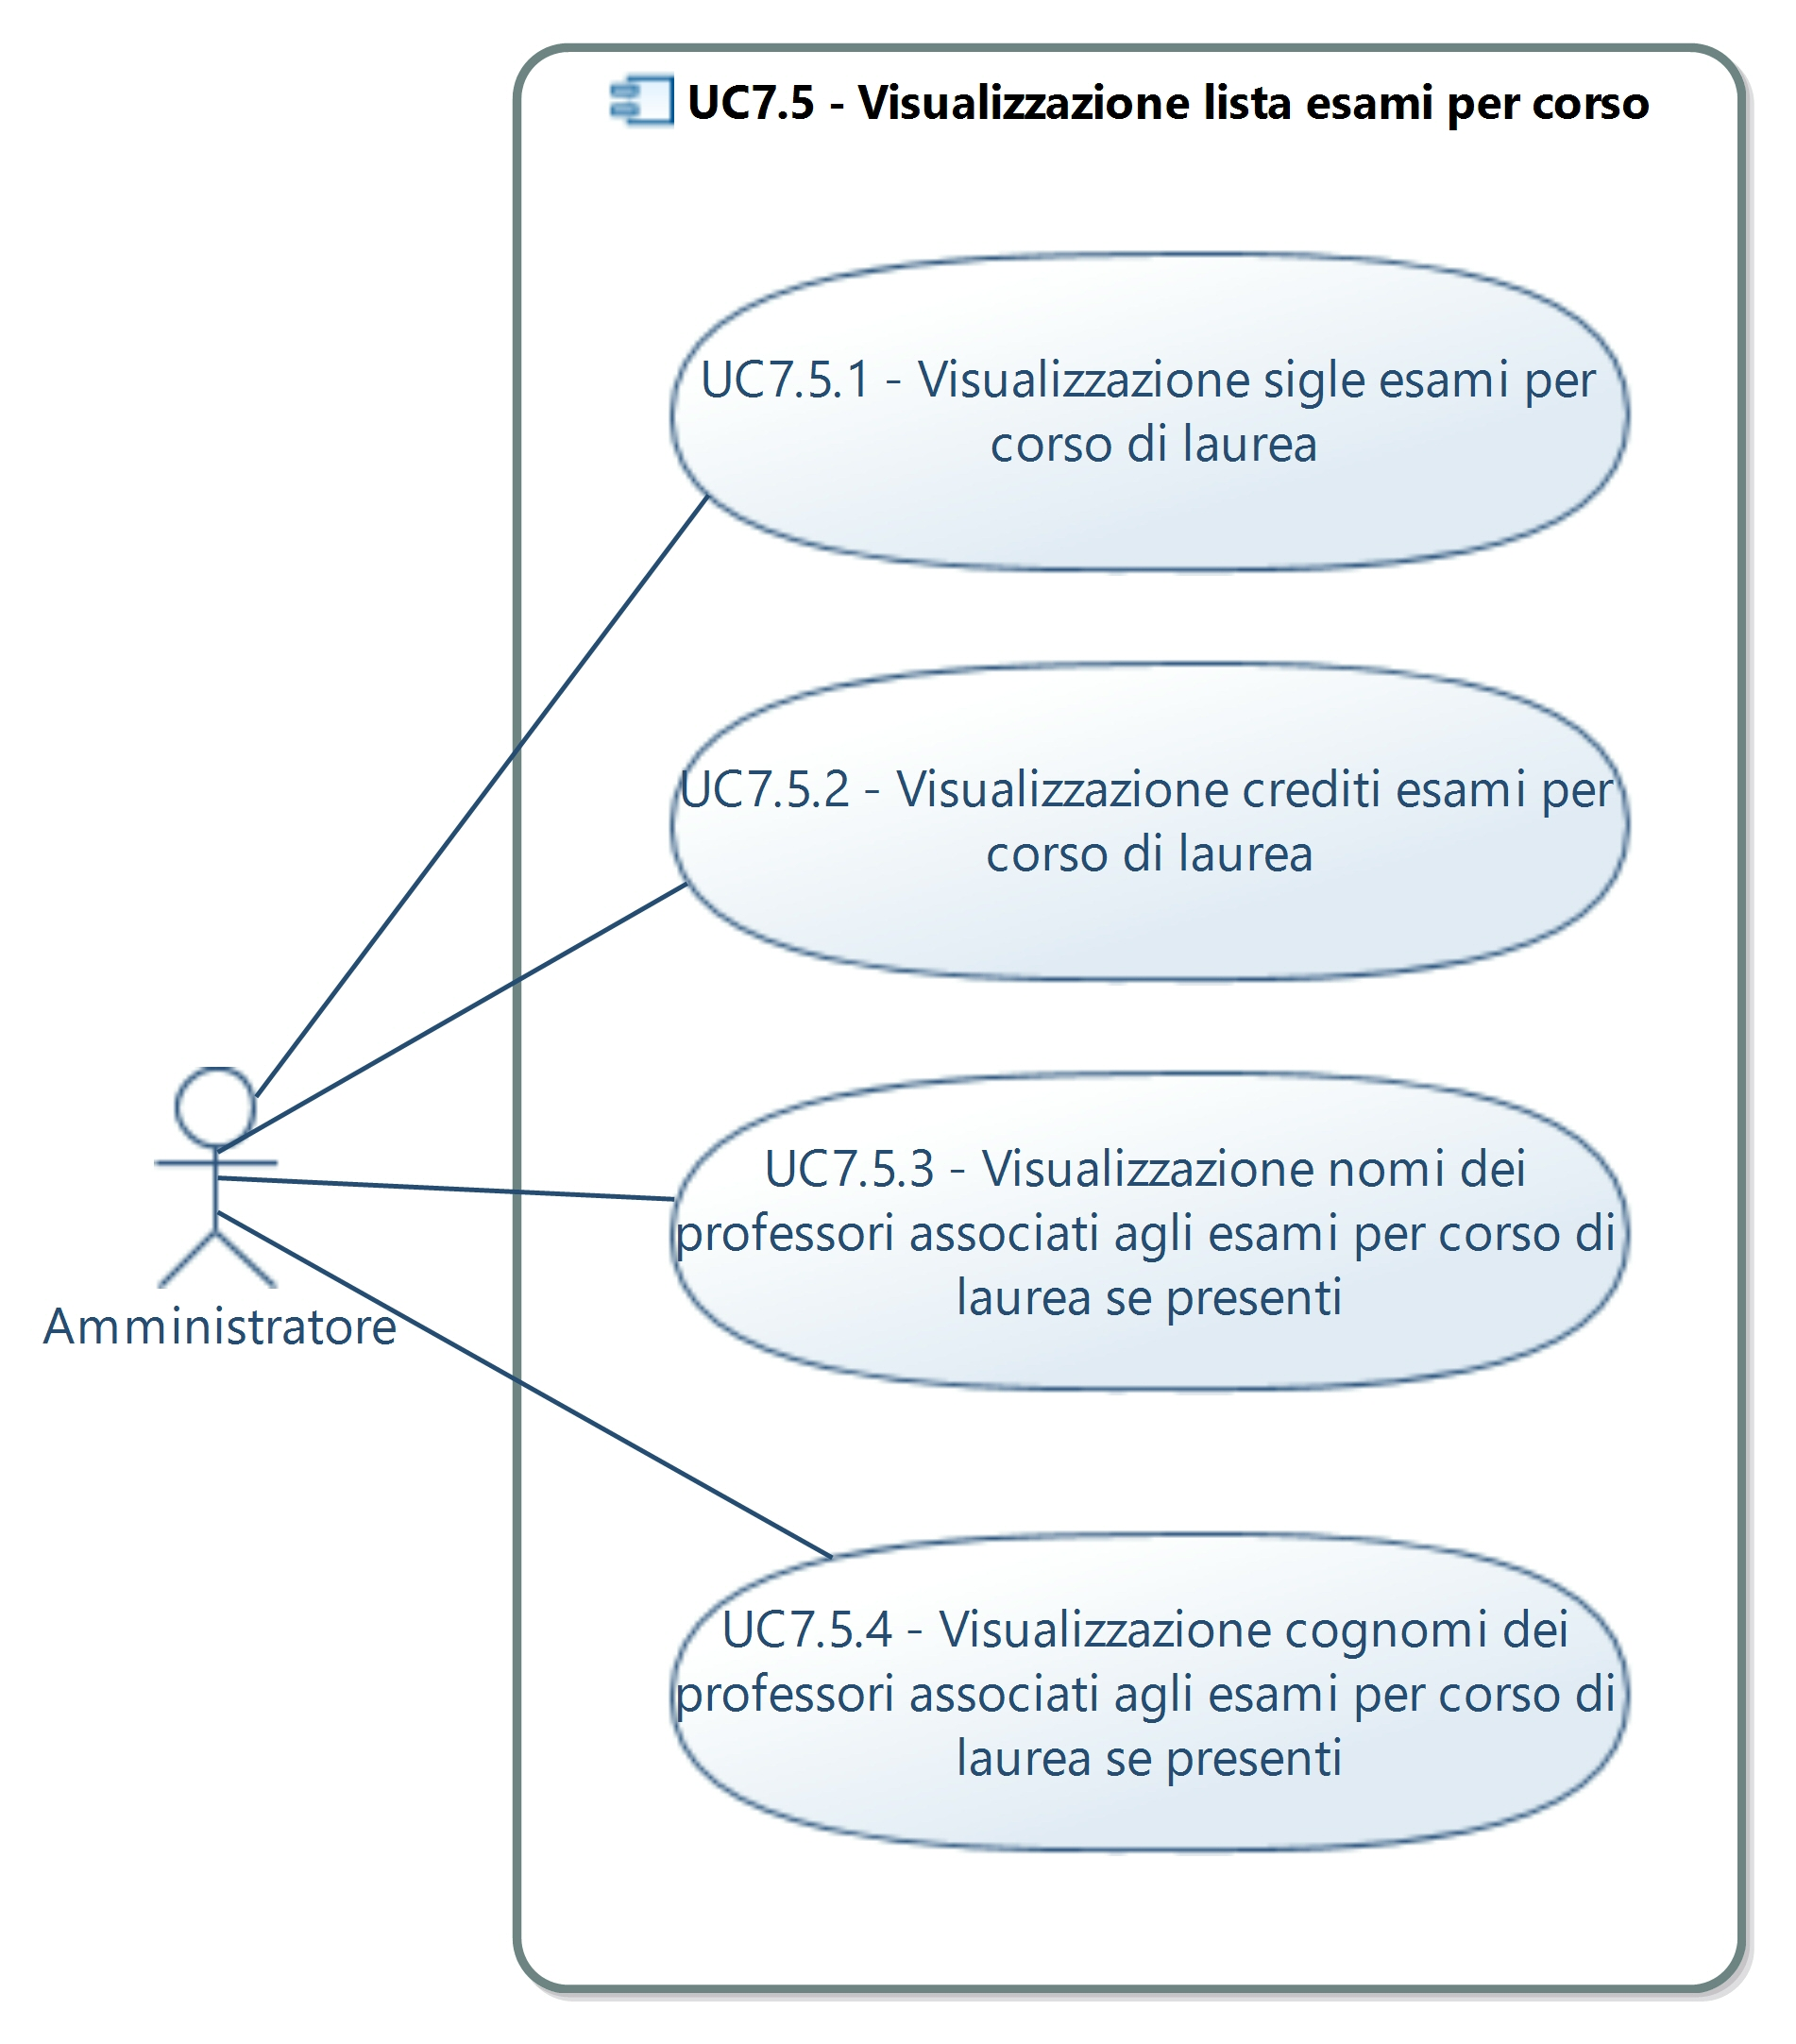
\includegraphics[width=0.8\linewidth]{UC7_5.jpg}
	\caption{UC7.5 - Visualizzazione lista esami per corso}
	\label{fig:UC7.5 - Visualizzazione lista esami per corso}
\end{figure}
\subsection{UC7.5.1 - Visualizzazione sigle esami per corso di laurea}
\begin{itemize}
	\item \textbf{Attori primari:} amministratore;
	\item \textbf{Scopo e descrizione:} l'amministratore visualizza la lista dei nomi degli esami presenti nel sistema per effettuare, eventualmente, delle operazioni su di esso;
	\item \textbf{Scenario principale:} il sistema mostra la lista di nomi degli esami associati a un determinato corso di laurea presenti nel sistema;
	\item \textbf{Precondizione:} il sistema riconosce l'utente come amministratore e riceve una richiesta di visualizzazione degli esami appartenenti a un determinato corso di laurea; 
	\item \textbf{Postcondizione:} il sistema fornisce all'amministratore la sigla di ogni esame presente nel corso di laurea indicatogli.
\end{itemize}
\subsection{UC7.5.2 - Visualizzazione crediti esami per corso di laurea}
\begin{itemize}
	\item \textbf{Attori primari:} amministratore;
	\item \textbf{Scopo e descrizione:} l'amministratore visualizza la lista dei crediti degli esami presenti nel sistema per effettuare, eventualmente, delle operazioni su di essa;
	\item \textbf{Scenario principale:} il sistema mostra la lista di crediti degli esami associati  un determinato corso di laurea presenti nel sistema;
	\item \textbf{Precondizione:} il sistema riconosce l'utente come amministratore e riceve una richiesta di visualizzazione degli esami appartenenti a un determinato corso di laurea; 
	\item \textbf{Postcondizione:} il sistema fornisce all'amministratore il numero di crediti relativi a ogni esame presente nel corso di laurea indicatogli.
\end{itemize}
\subsection{UC7.5.3 - Visualizzazione nomi dei professori associati agli esami per corso di laurea se presenti}
\begin{itemize}
	\item \textbf{Attori primari:} amministratore;
	\item \textbf{Scopo e descrizione:} l'amministratore visualizza la lista dei nomi dei professori degli esami presenti nel sistema per effettuare, eventualmente, delle operazioni su di esso;
	\item \textbf{Scenario principale:} il sistema mostra la lista di nomi dei professori degli esami associati a un determinato corso di laurea presenti nel sistema;
	\item \textbf{Precondizione:} il sistema riconosce l'utente come amministratore e riceve una richiesta di visualizzazione degli esami appartenenti a un determinato corso di laurea; 
	\item \textbf{Postcondizione:} il sistema fornisce per ogni esame presente nel corso di laurea indicatogli il nome del professore assegnato.
\end{itemize}
\subsection{UC7.5.4 - Visualizzazione cognomi dei professori associati agli esami per corso di laurea se presenti}
\begin{itemize}
	\item \textbf{Attori primari:} amministratore;
	\item \textbf{Scopo e descrizione:} l'amministratore visualizza la lista dei cognomi dei professori degli esami presenti nel sistema per effettuare, eventualmente, delle operazioni su di esso;
	\item \textbf{Scenario principale:} il sistema mostra la lista di cognomi dei professori degli esami associati a un determinato corso di laurea presenti nel sistema;
	\item \textbf{Precondizione:} il sistema riconosce l'utente come amministratore e riceve una richiesta di visualizzazione degli esami appartenenti a un determinato corso di laurea; 
	\item \textbf{Postcondizione:} il sistema fornisce per ogni esame presente nel corso di laurea indicatogli il cognome del professore assegnato.
\end{itemize}
\subsection{UC7.6 - Visualizzazione lista esami}
\begin{itemize}
	\item \textbf{Attori primari:} amministratore;
	\item \textbf{Scopo e descrizione:} vengono visualizzati gli esami all'interno del sistema, con indicato per ognuno di essi il nome, il numero di crediti, la sigla del corso a esso associato e, se presente, il nome e il cognome del professore assegnatogli;
	\item \textbf{Scenario principale:} l'amministratore visualizza la lista di tutti gli esami presenti nel sistema;
	\item \textbf{Precondizione:} il sistema riconosce l'utente come amministratore e fornisce la lista delle funzionalità alle quali ha accesso relative all'amministrazione dei corsi di laurea;
	\item \textbf{Postcondizione:} il sistema fornisce all'utente riconosciuto come amministratore la lista degli esami.
\end{itemize}
\begin{figure}[H]
	\centering
	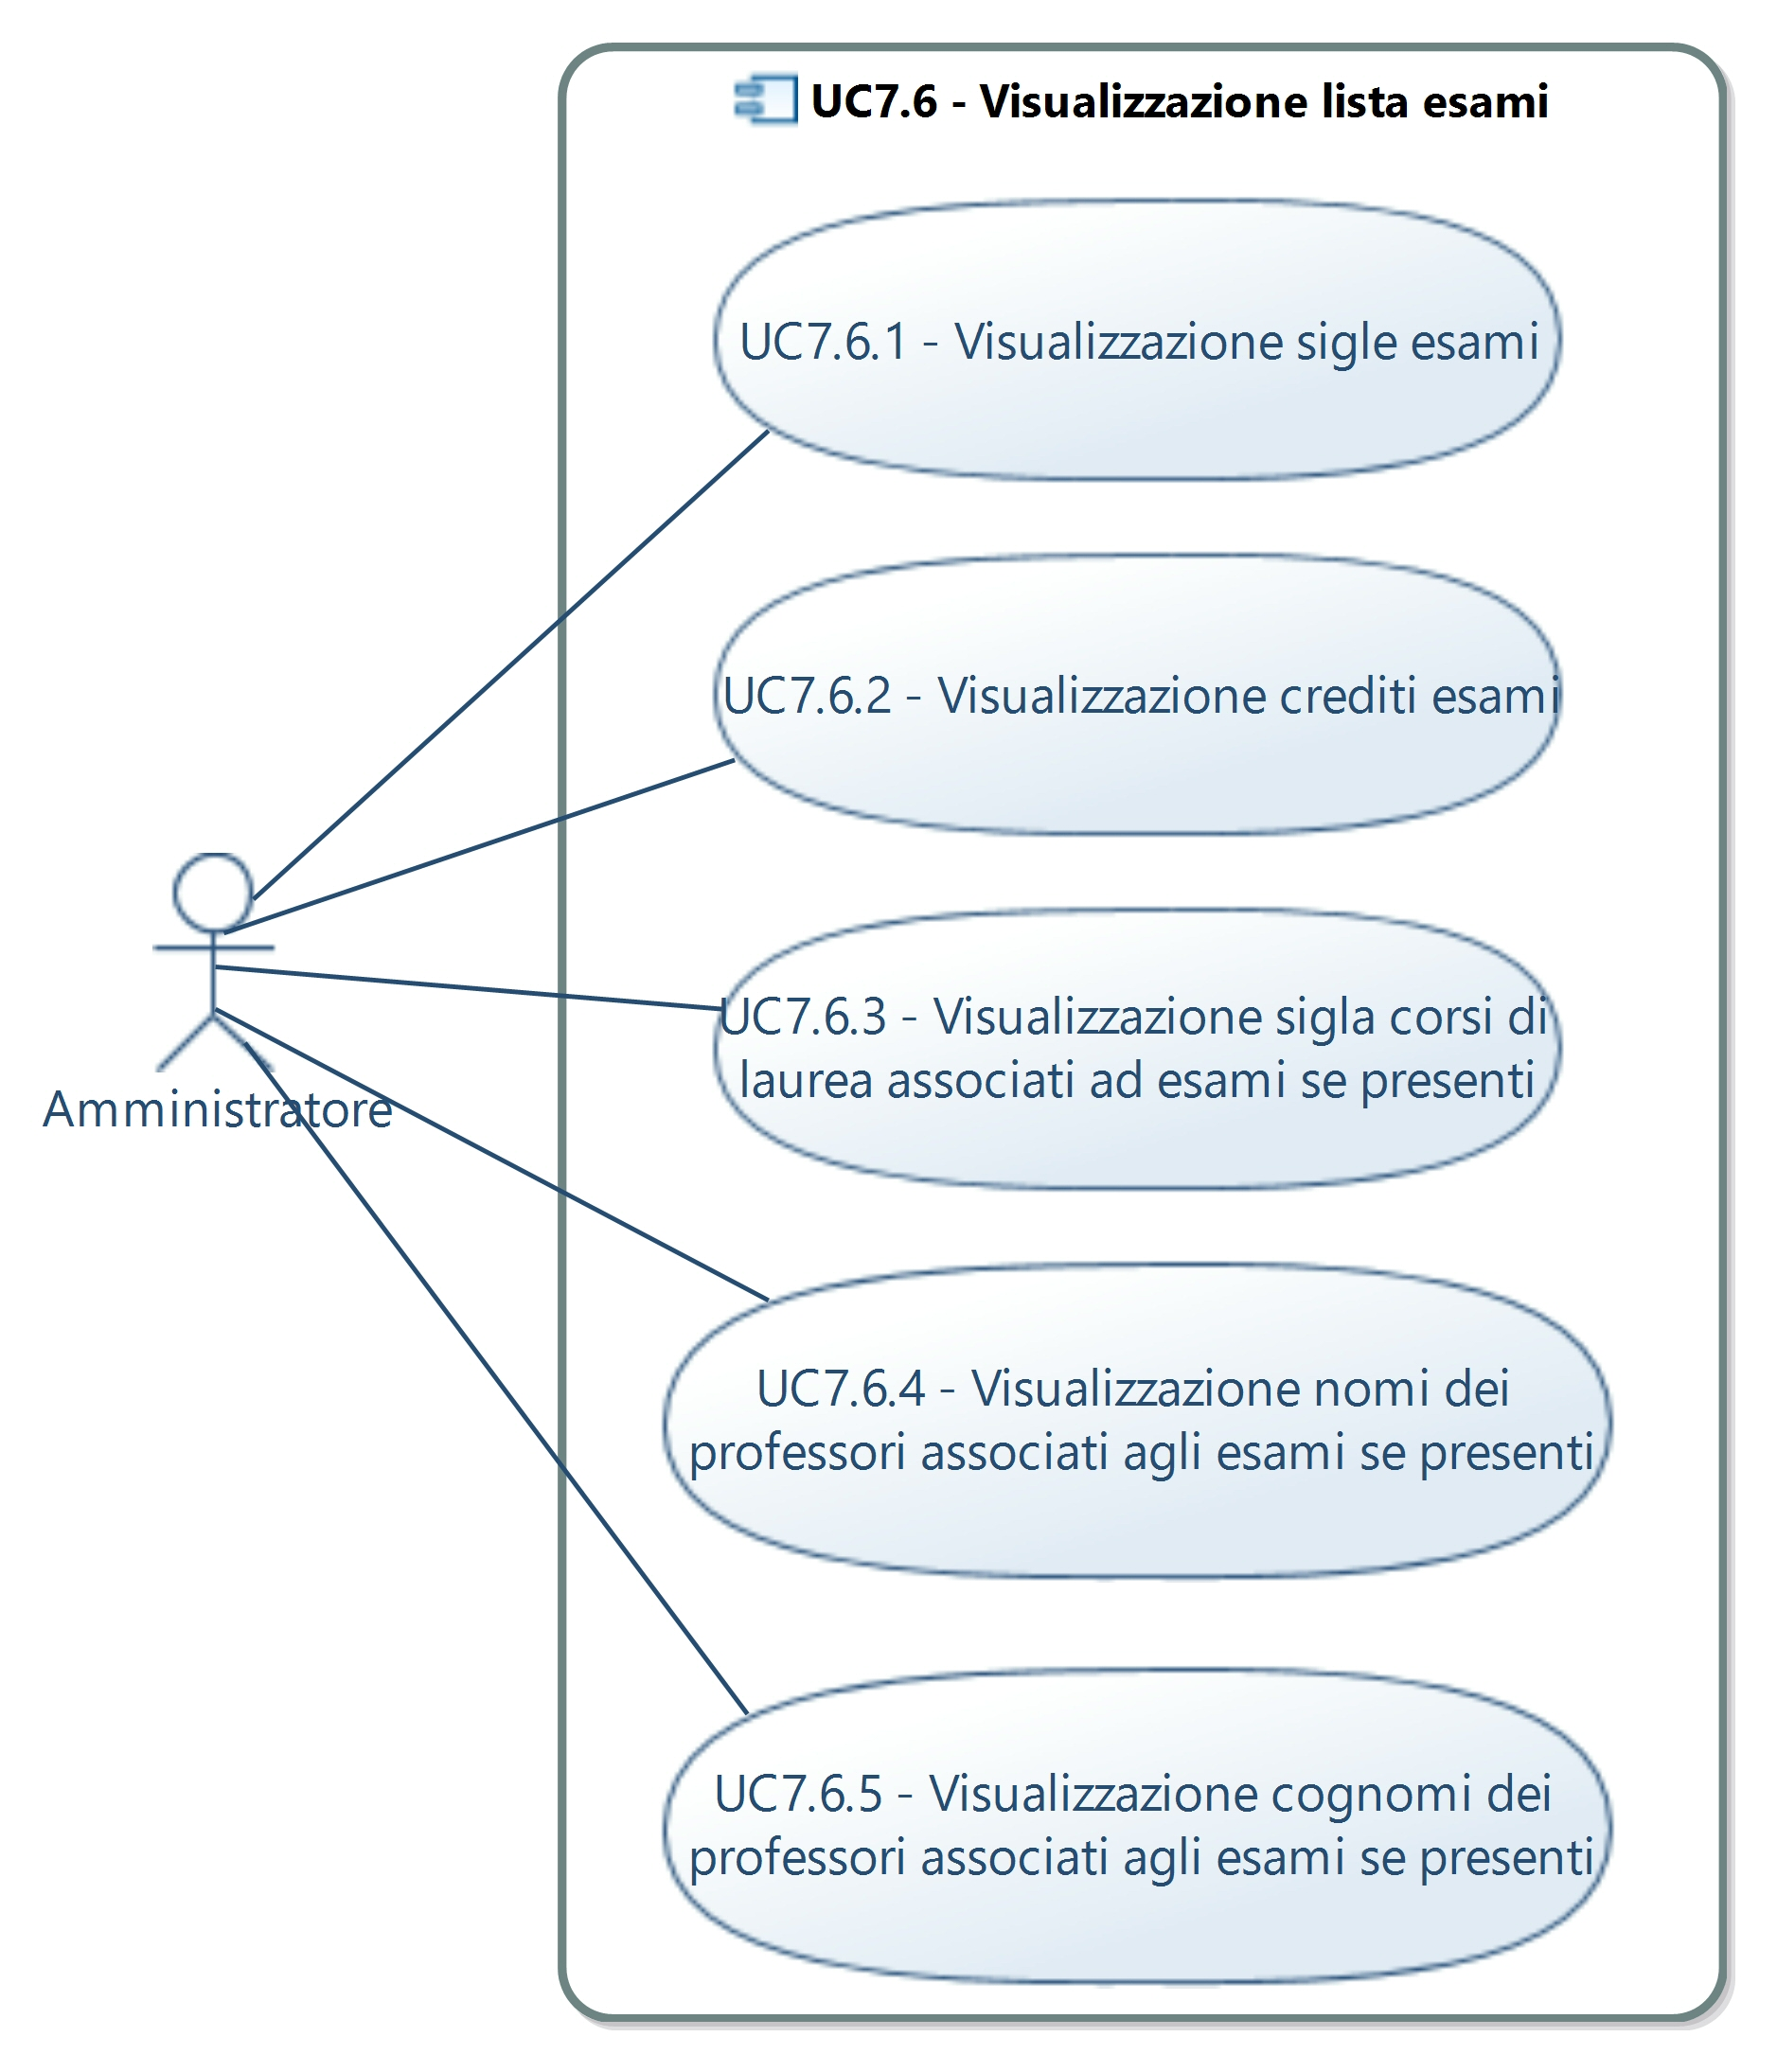
\includegraphics[width=0.7\linewidth]{UC7_6.jpg}
	\caption{UC7.6 - Visualizzazione lista esami}
	\label{fig:UC7.6 - Visualizzazione lista esami}
\end{figure}
\subsection{UC7.6.1 - Visualizzazione sigla esami}
\begin{itemize}
	\item \textbf{Attori primari:} amministratore;
	\item \textbf{Scopo e descrizione:} l'amministratore visualizza la lista dei nomi degli esami presenti nel sistema per effettuare, eventualmente, delle operazioni su di essa;
	\item \textbf{Scenario principale:} il sistema mostra la lista di nomi degli esami presenti nel sistema;
	\item \textbf{Precondizione:} il sistema riconosce l'utente come amministratore e riceve una richiesta di visualizzazione di tutti gli esami; 
	\item \textbf{Postcondizione:} il sistema fornisce all'amministratore la sigla di ogni esame presente nel sistema.
\end{itemize}
\subsection{UC7.6.2 - Visualizzazione crediti esami}
\begin{itemize}
	\item \textbf{Attori primari:} amministratore;
	\item \textbf{Scopo e descrizione:} l'amministratore visualizza la lista dei crediti degli esami presenti nel sistema per effettuare, eventualmente, delle operazioni su di esso;
	\item \textbf{Scenario principale:} il sistema mostra la lista di crediti degli esami presenti nel sistema;
	\item \textbf{Precondizione:} il sistema riconosce l'utente come amministratore e riceve una richiesta di visualizzazione di tutti gli esami; 
	\item \textbf{Postcondizione:} il sistema fornisce all'amministratore il numero di crediti relativi a ogni esame presente.
\end{itemize}
\subsection{UC7.6.3 - Visualizzazione sigla corsi di laurea associati a esami se presenti}
\begin{itemize}
	\item \textbf{Attori primari:} amministratore;
	\item \textbf{Scopo e descrizione:} l'amministratore visualizza la lista delle sigle dei corsi di laurea associati agli esami presenti nel sistema per effettuare, eventualmente, delle operazioni su di esso;
	\item \textbf{Scenario principale:} il sistema mostra la lista delle sigle dei corsi di laurea associati agli esami presenti nel sistema;
	\item \textbf{Precondizione:} il sistema riconosce l'utente come amministratore e riceve una richiesta di visualizzazione di tutti gli esami;  
	\item \textbf{Postcondizione:} il sistema fornisce per ogni esame presente la sigla del corso di laurea che lo contiene.
\end{itemize}
\subsection{UC7.6.4 - Visualizzazione nomi dei professori associati agli esami se presenti}
\begin{itemize}
	\item \textbf{Attori primari:} amministratore;
	\item \textbf{Scopo e descrizione:} l'amministratore visualizza la lista dei nomi dei professori degli esami presenti nel sistema per effettuare, eventualmente, delle operazioni su di essa;
	\item \textbf{Scenario principale:} il sistema mostra la lista di nomi dei professori degli esami presenti nel sistema;
	\item \textbf{Precondizione:} il sistema riconosce l'utente come amministratore e riceve una richiesta di visualizzazione di tutti gli esami; 
	\item \textbf{Postcondizione:} il sistema fornisce per ogni esame il nome del professore assegnato.
\end{itemize}
\subsection{UC7.6.5 - Visualizzazione cognomi dei professori associati agli esami se presenti}
\begin{itemize}
	\item \textbf{Attori primari:} amministratore;
	\item \textbf{Scopo e descrizione:} l'amministratore visualizza la lista dei cognomi dei professori degli esami presenti nel sistema per effettuare, eventualmente, delle operazioni su di essa;
	\item \textbf{Scenario principale:} il sistema mostra la lista di cognomi dei professori degli esami presenti nel sistema;
	\item \textbf{Precondizione:} il sistema riconosce l'utente come amministratore e riceve una richiesta di visualizzazione di tutti gli esami; 
	\item \textbf{Postcondizione:} il sistema fornisce per ogni esame il cognome del professore assegnato.
\end{itemize}
\subsection{UC7.7 - Visualizzazione dettagli esame}
\begin{itemize}
	\item \textbf{Attori primari:} amministratore;
	\item \textbf{Scopo e descrizione:} l'amministratore visualizza i dettagli dell'esame indicato;
	\item \textbf{Scenario principale:}
	\begin{enumerate}
		\item L'amministratore ottiene una lista degli esami e seleziona quello di suo interesse [UC7.5 o UC7.6];
		\item Il sistema mostra una schermata informativa contenente i dati relativi all'esame [UC7.7].
	\end{enumerate}
	\item \textbf{Precondizione:} il sistema riconosce l'utente come amministratore e ha precedentemente fornito un elenco di esami [UC7.5 o UC7.6]; 
	\item \textbf{Postcondizione:} il sistema fornisce all'amministratore informazioni maggiormente dettagliare riguardanti un esame richiesto.
\end{itemize}
\begin{figure}[H]
	\centering
	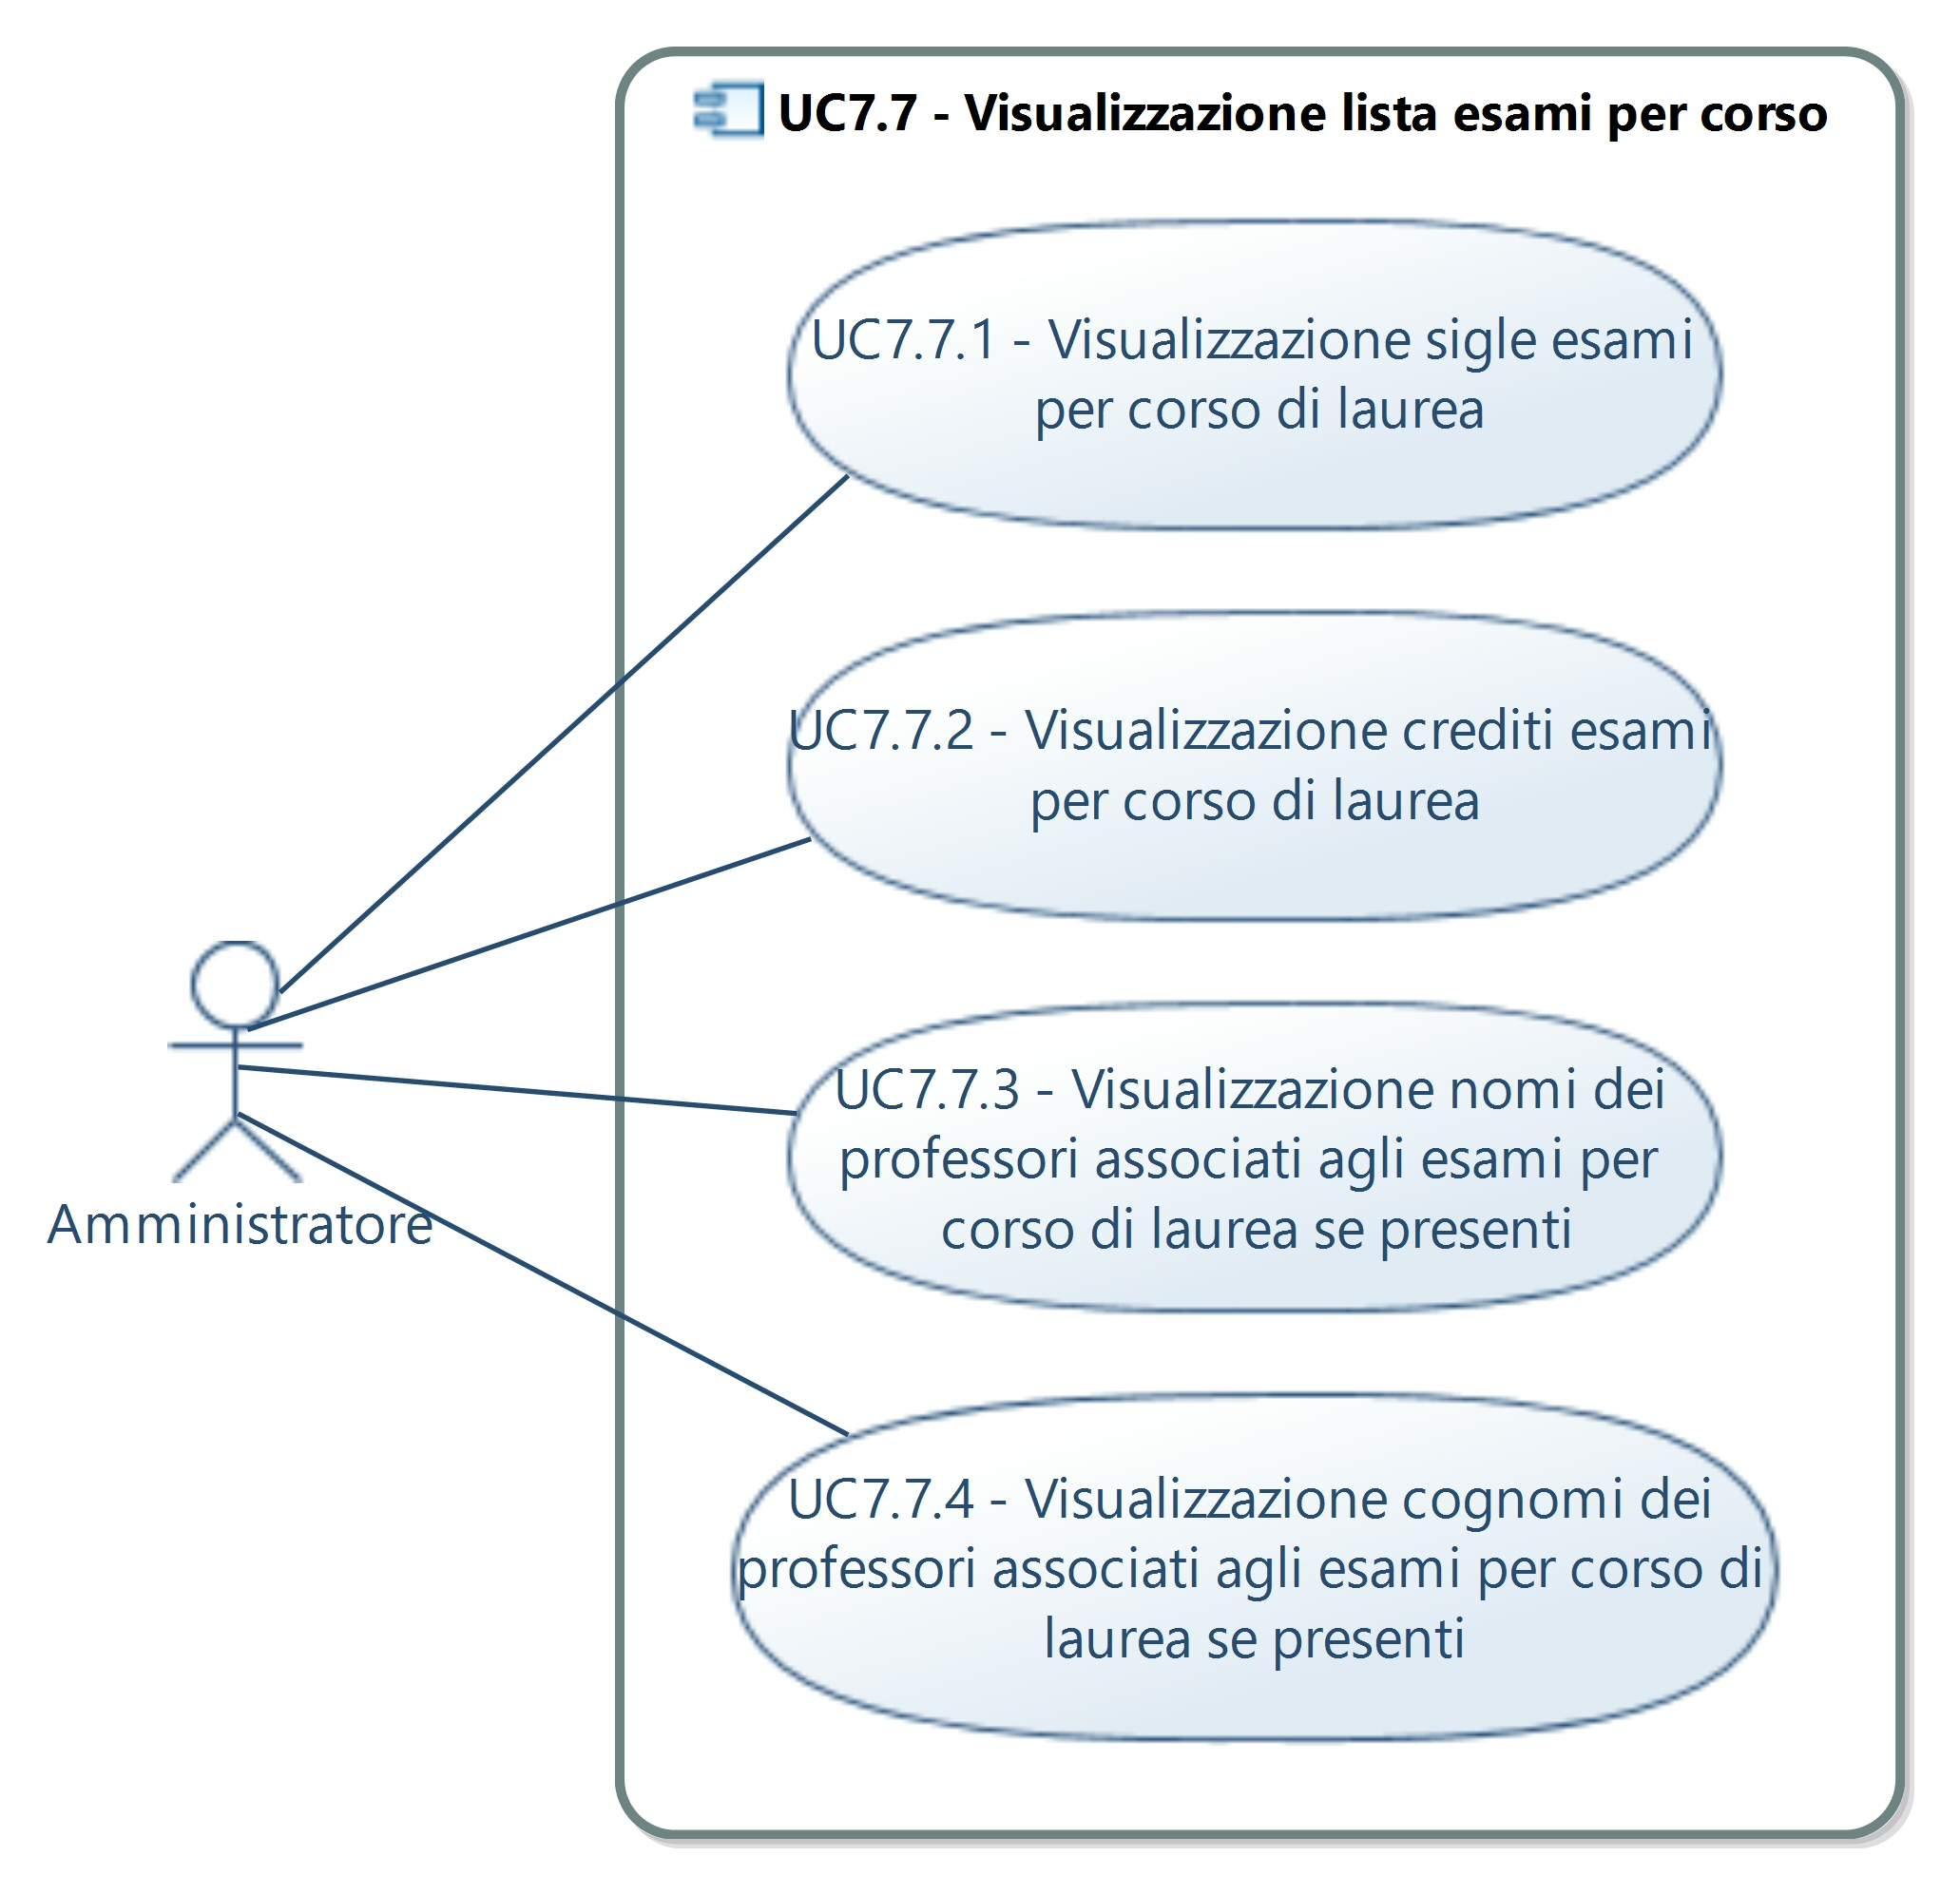
\includegraphics[width=1\linewidth]{UC7_7.jpg}
	\caption{UC7.7 - Visualizzazione dettagli esame}
	\label{fig:UC7.7 - Visualizzazione dettagli esame}
\end{figure}
\subsection{UC7.7.1 - Visualizzazione sigla esame}
\begin{itemize}
	\item \textbf{Attori primari:} amministratore;
	\item \textbf{Scopo e descrizione:} l'amministratore vuole visualizzare il nome dell'esame per effettuare, eventualmente, delle operazioni su di esso;
	\item \textbf{Scenario principale:} l'amministratore visualizza il nome dell'esame;
	\item \textbf{Precondizione:} il sistema riconosce l'utente come amministratore e quest'ultimo richiede la visualizzazione dei dettagli relativi a un esame; 
	\item \textbf{Postcondizione:} il sistema visualizza la sigla dell'esame indicato.
\end{itemize}
\subsection{UC7.7.2 - Visualizzazione crediti esame}
\begin{itemize}
	\item \textbf{Attori primari:} amministratore;
	\item \textbf{Scopo e descrizione:} l'amministratore vuole visualizzare i crediti dell'esame per effettuare, eventualmente, delle operazioni su di esso;
	\item \textbf{Scenario principale:} l'amministratore visualizza i crediti dell'esame;
	\item \textbf{Precondizione:} il sistema riconosce l'utente come amministratore e quest'ultimo richiede la visualizzazione dei dettagli relativi a un esame; 
	\item \textbf{Postcondizione:} il sistema visualizza i crediti dell'esame indicato.
\end{itemize}
\subsection{UC7.7.3 - Visualizzazione corso di laurea associato all'esame se presente}
\begin{itemize}
	\item \textbf{Attori primari:} amministratore;
	\item \textbf{Scopo e descrizione:} l'amministratore vuole visualizzare il nome del corso di laurea associato all'esame per effettuare, eventualmente, delle operazioni su di esso;
	\item \textbf{Scenario principale:} l'amministratore visualizza il nome del corso di laurea associato all'esame;
	\item \textbf{Precondizione:} il sistema riconosce l'utente come amministratore e quest'ultimo richiede la visualizzazione dei dettagli relativi a un esame; 
	\item \textbf{Postcondizione:} il sistema visualizza il corso di laurea al quale appartiene l'esame indicato.
\end{itemize}
\subsection{UC7.7.4 - Visualizzazione nome del professore associato all'esame se presente}
\begin{itemize}
	\item \textbf{Attori primari:} amministratore;
	\item \textbf{Scopo e descrizione:} l'amministratore vuole visualizzare il nome del professore associato all'esame per effettuare, eventualmente, delle operazioni su di esso;
	\item \textbf{Scenario principale:} l'amministratore visualizza il nome del professore associato all'esame;
	\item \textbf{Precondizione:} il sistema riconosce l'utente come amministratore e quest'ultimo richiede la visualizzazione dei dettagli relativi a un esame; 
	\item \textbf{Postcondizione:} il sistema visualizza il nome del professore assegnato all'esame indicato.
\end{itemize}
\subsection{UC7.7.5 - Visualizzazione cognome del professore associato all'esame se presente}
\begin{itemize}
	\item \textbf{Attori primari:} amministratore;
	\item \textbf{Scopo e descrizione:} l'amministratore vuole visualizzare il cognome del professore associato all'esame per effettuare, eventualmente, delle operazioni su di esso;
	\item \textbf{Scenario principale:} l'amministratore visualizza il cognome del professore associato all'esame;
	\item \textbf{Precondizione:} il sistema riconosce l'utente come amministratore e quest'ultimo richiede la visualizzazione dei dettagli relativi a un esame; 
	\item \textbf{Postcondizione:} il sistema visualizza il cognome del professore assegnato all'esame indicato.
\end{itemize}
\subsection{UC7.7.6 - Visualizzazione numero di studenti iscritti all'esame}
\begin{itemize}
	\item \textbf{Attori primari:} amministratore;
	\item \textbf{Scopo e descrizione:} l'amministratore vuole visualizzare il numero di studenti iscritti all'esame per effettuare, eventualmente, delle operazioni su di esso;
	\item \textbf{Scenario principale:} l'amministratore visualizza il numero di studenti iscritti all'esame;
	\item \textbf{Precondizione:} il sistema riconosce l'utente come amministratore e quest'ultimo richiede la visualizzazione dei dettagli relativi a un esame; 
	\item \textbf{Postcondizione:} il sistema visualizza il numero di studenti iscritti all'esame indicato.
\end{itemize}
\subsection{UC7.7.7 - Visualizzazione indirizzo del professore associato all'esame se presente}
\begin{itemize}
	\item \textbf{Attori primari:} amministratore;
	\item \textbf{Scopo e descrizione:} l'amministratore vuole visualizzare l'indirizzo del professore associato all'esame per effettuare, eventualmente, delle operazioni su di esso;
	\item \textbf{Scenario principale:} l'amministratore visualizza l'indirizzo del professore associato all'esame;
	\item \textbf{Precondizione:} il sistema riconosce l'utente come amministratore e quest'ultimo richiede la visualizzazione dei dettagli relativi a un esame; 
	\item \textbf{Postcondizione:} il sistema visualizza l'indirizzo del professore assegnato all'esame indicato.
\end{itemize}
\subsection{UC7.8 - Visualizzazione di tutti gli anni accademici}
\begin{itemize}
	\item \textbf{Attori primari:} amministratore;
	\item \textbf{Scopo e descrizione:} l'utente è già riconosciuto dal sistema come amministratore e visualizza una lista di tutti gli anni accademici presenti nel sistema, visualizzandone l'anno solare di riferimento;
	\item \textbf{Scenario principale:} l'amministratore richiede la lista di tutti gli anni del sistema;
	\item \textbf{Precondizione:} il sistema riconosce l'utente come amministratore e fornisce la lista delle funzionalità alle quali ha accesso relative all'amministrazione dei corsi di laurea;
	\item \textbf{Postcondizione:} il sistema fornisce la lista di tutti gli anni accademici presenti nel sistema.
\end{itemize}
\begin{figure}[H]
	\centering
	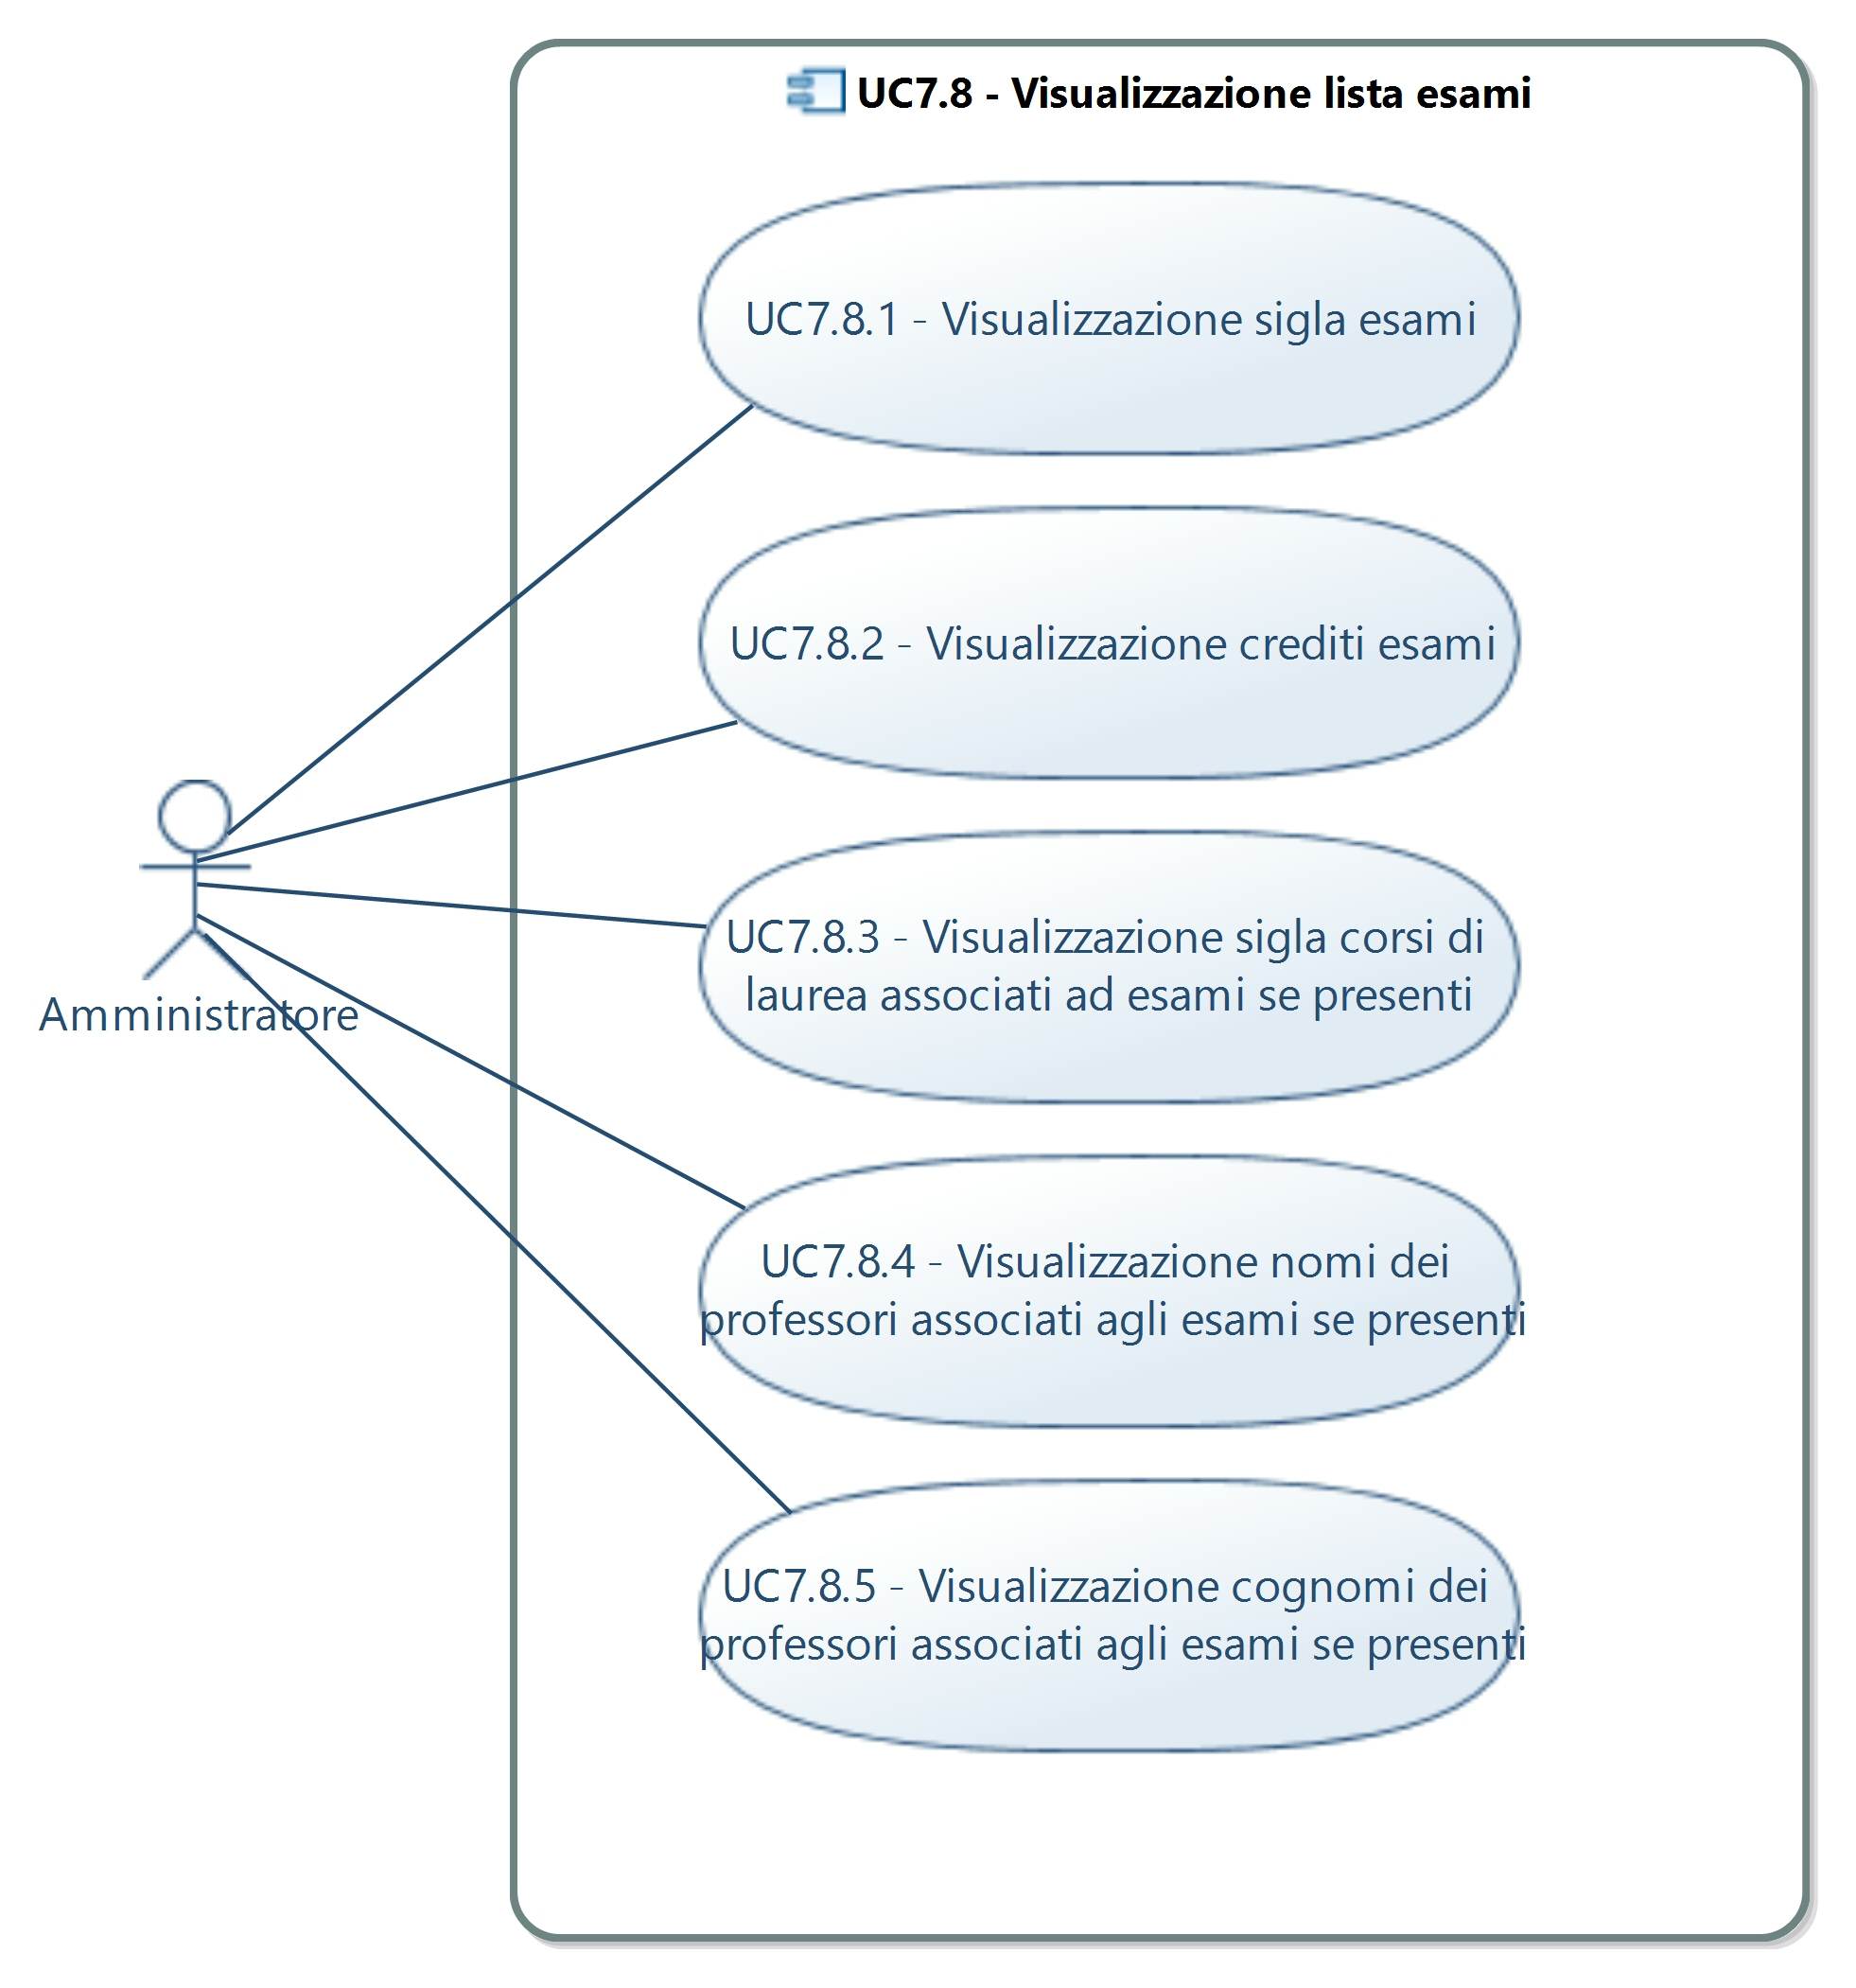
\includegraphics[width=0.7\linewidth]{UC7_8.jpg}
	\caption{UC7.8 - Visualizzazione di tutti gli anni accademici}
	\label{UC7.8 - Visualizzazione di tutti gli anni accademici}
\end{figure}
\subsection{UC7.8.1 - Visualizzazione anni solari relativi agli anni accademici}
\begin{itemize}
	\item \textbf{Attori primari:} amministratore;
	\item \textbf{Scopo e descrizione:} l'utente già riconosciuto dal sistema come amministratore visualizza una lista di tutti gli anni solari relativi agli anni accademici inseriti nella rete \citGloss{Ethereum};
	\item \textbf{Scenario principale:} l'amministratore richiede al sistema la lista di anni accademici inseriti nel sistema per visualizzarli ed eventualmente compiere operazioni su di essi;
	\item \textbf{Precondizione:} il sistema riconosce l'utente come amministratore, il quale richiede la lista di tutti gli anni accademici presenti nel sistema;
	\item \textbf{Postcondizione:} il sistema, per ogni anno accademico, visualizza il relativo anno solare.
\end{itemize}
\subsection{UC7.9 - Visualizzazione lista professori da associare a un esame}
\begin{itemize}
	\item \textbf{Attori primari:} amministratore;
	\item \textbf{Scopo e descrizione:} l'amministratore visualizza una lista dei nomi, cognomi e indirizzi dei professori per identificare quale assegnare all'esame precedentemente indicato;
	\item \textbf{Scenario principale:} il sistema mostra all'amministratore una lista di professori in modo da consentire la scelta di quale associare all'esame precedentemente indicato;
	\item \textbf{Precondizione:} il sistema riconosce l'utente come amministratore e fornisce la lista degli esami [UC7.6];  
	\item \textbf{Postcondizione:} il sistema fornisce all'amministratore la lista dei professori per permettere l'assegnazione di uno di essi a un dato esame indicato dall'utente.
\end{itemize}
\begin{figure}[H]
	\centering
	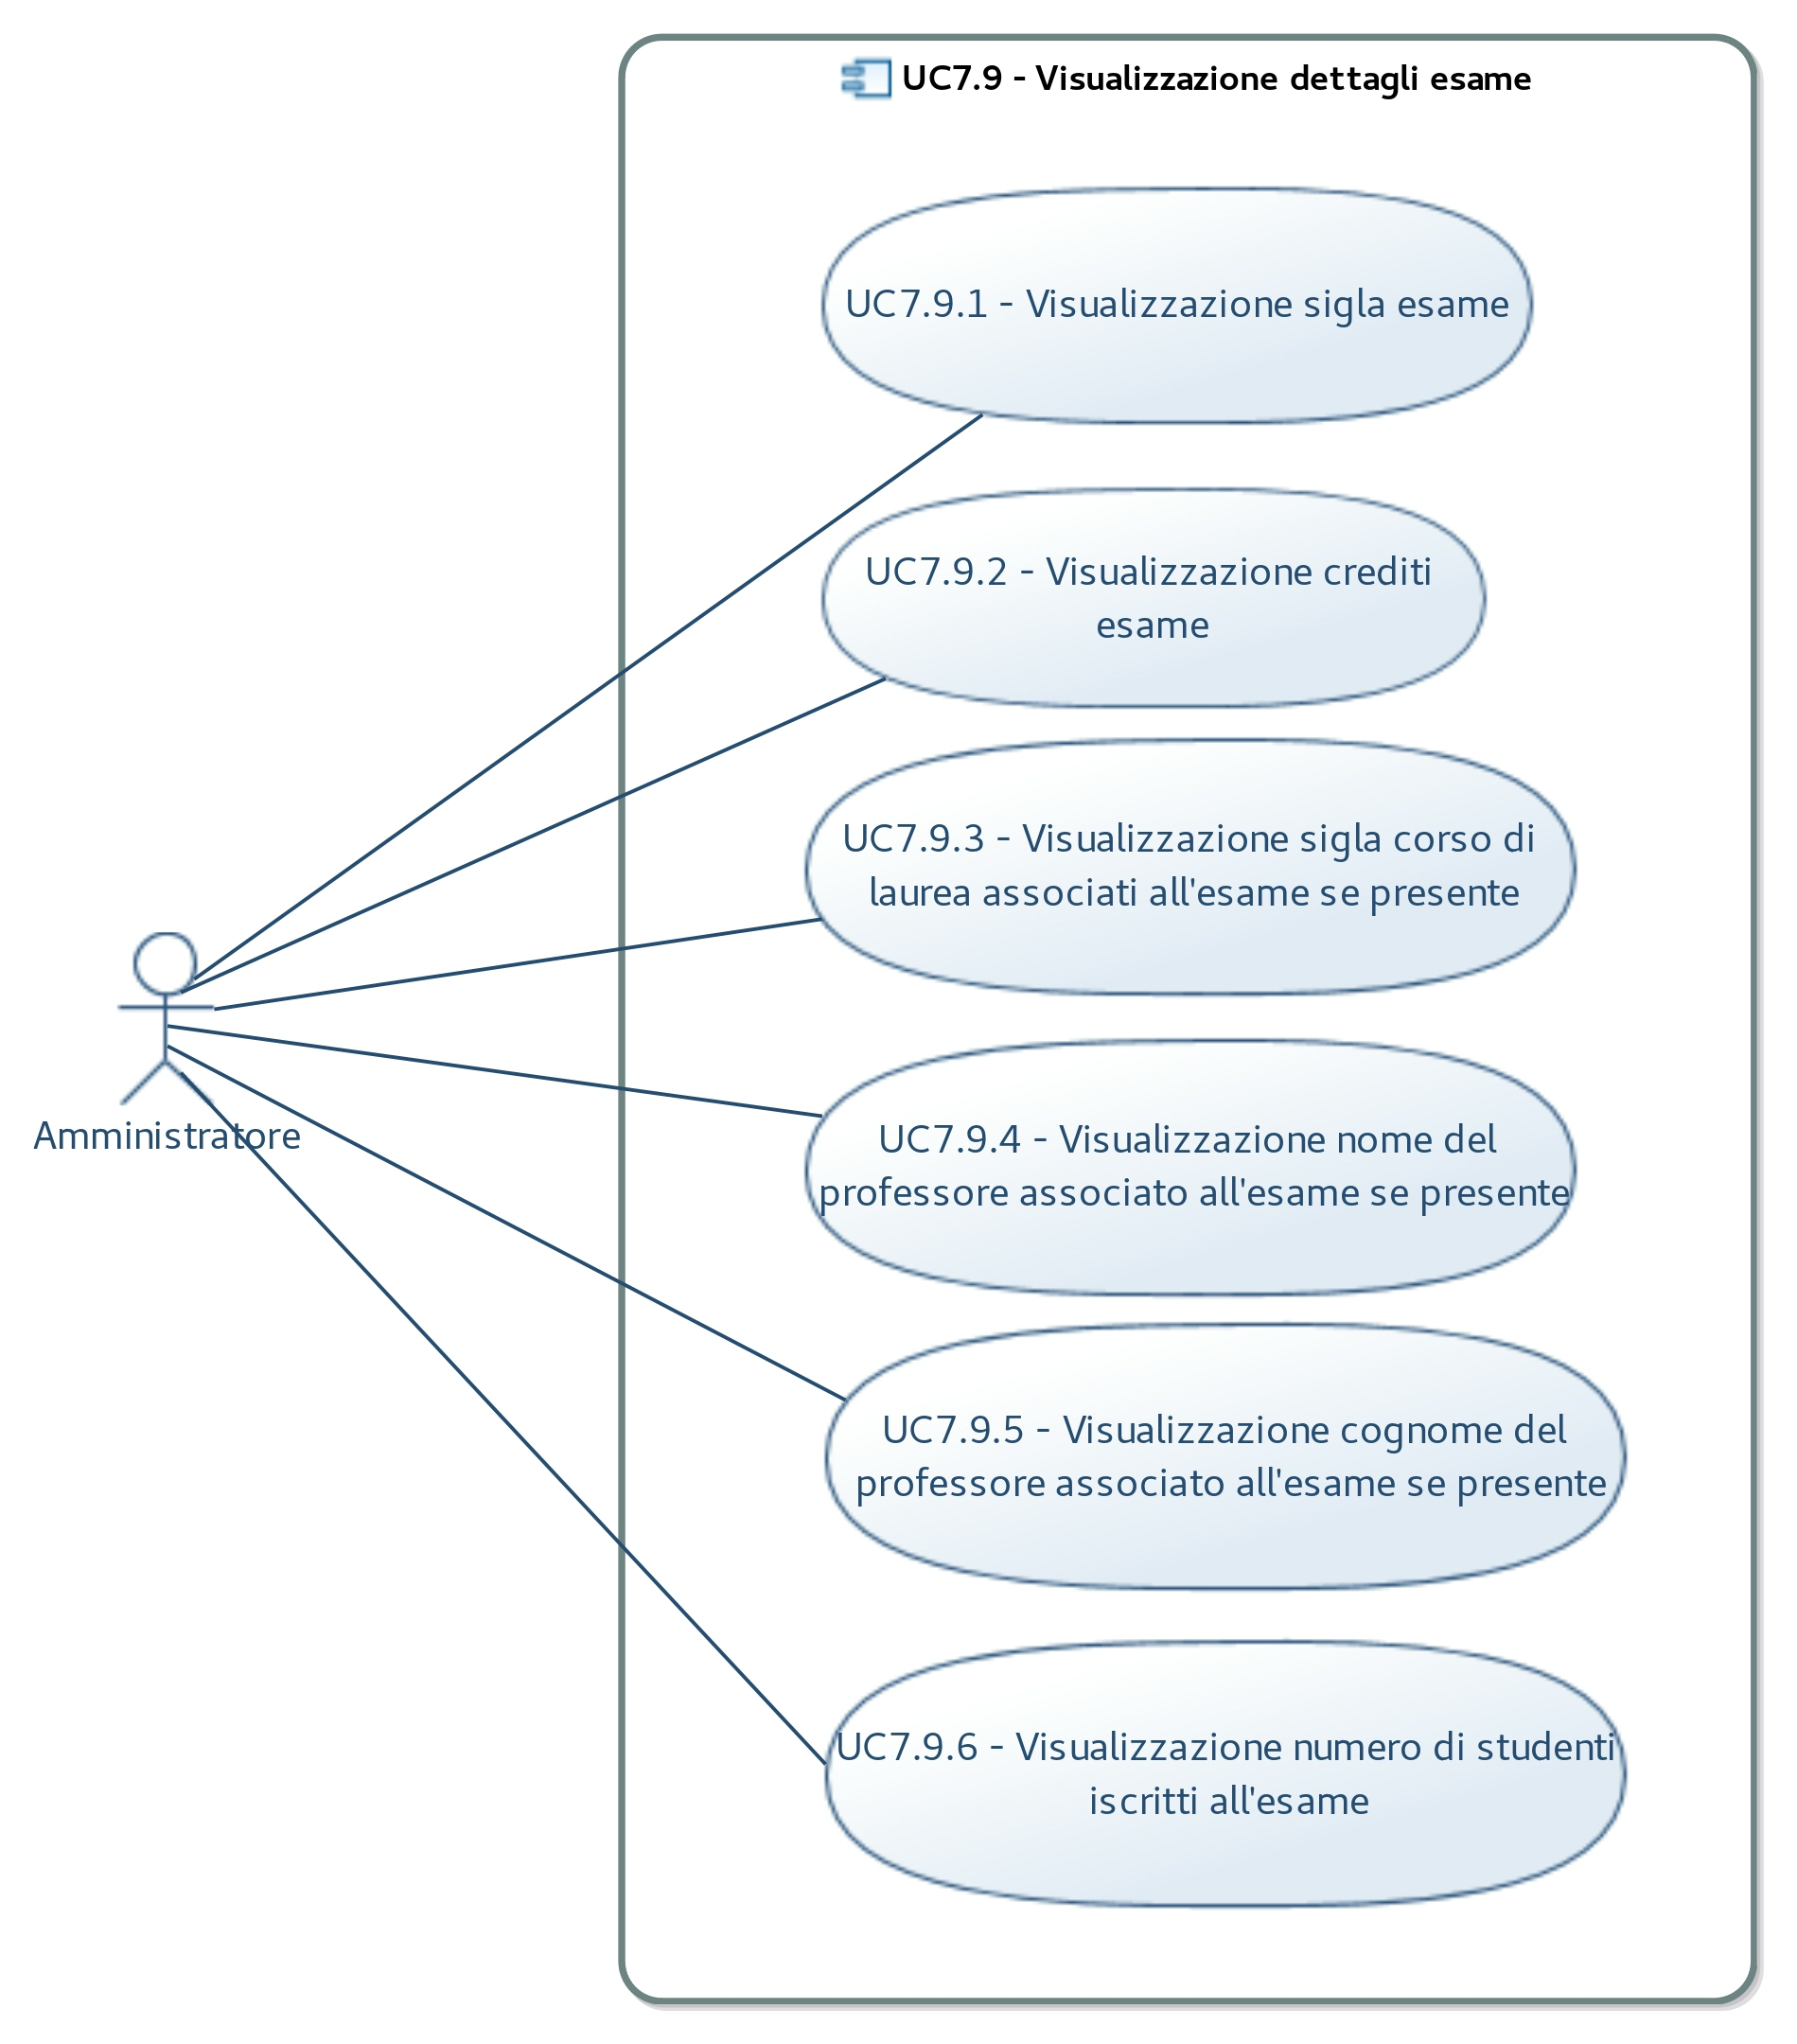
\includegraphics[width=0.7\linewidth]{UC7_9.jpg}
	\caption{UC7.9 - Visualizzazione lista professori da associare a un esame}
	\label{UC7.9 - Visualizzazione lista professori da associare a un esame}
\end{figure}
\subsection{UC7.9.1 - Visualizzazione nome per ogni professore}
\begin{itemize}
	\item \textbf{Attori primari:} amministratore;
	\item \textbf{Scopo e descrizione:} l'amministratore visualizza la lista dei nomi dei professori degli esami presenti nel sistema per poter determinare quale associare all'esame precedentemente indicato;
	\item \textbf{Scenario principale:} all'amministratore viene fornita la lista dei nomi dei professori presenti nel sistema;
	\item \textbf{Precondizione:} il sistema riconosce l'utente come amministratore e riceve una richiesta di visualizzazione dei professori per poterne assegnare uno a un dato esame precedentemente indicato; 
	\item \textbf{Postcondizione:} il sistema fornisce per ogni professore il relativo nome.
\end{itemize}
\subsection{UC7.9.2 - Visualizzazione cognome per ogni professore}
\begin{itemize}
	\item \textbf{Attori primari:} amministratore;
	\item \textbf{Scopo e descrizione:} l'amministratore visualizza la lista dei cognomi dei professori degli esami presenti nel sistema per poter determinare quale associare all'esame precedentemente indicato;
	\item \textbf{Scenario principale:} all'amministratore viene fornita la lista dei cognomi dei professori presenti nel sistema;
	\item \textbf{Precondizione:} il sistema riconosce l'utente come amministratore e riceve una richiesta di visualizzazione dei professori per poterne assegnare uno a un dato esame precedentemente indicato; 
	\item \textbf{Postcondizione:} il sistema fornisce per ogni professore il relativo cognome.
\end{itemize}
\subsection{UC7.9.3 - Visualizzazione indirizzo per ogni professore}
\begin{itemize}
	\item \textbf{Attori primari:} amministratore;
	\item \textbf{Scopo e descrizione:} l'amministratore visualizza la lista degli indirizzi dei professori degli esami presenti nel sistema per poter determinare quale associare all'esame precedentemente indicato;
	\item \textbf{Scenario principale:} all'amministratore viene fornita la lista degli indirizzi dei professori presenti nel sistema;
	\item \textbf{Precondizione:} il sistema riconosce l'utente come amministratore e riceve una richiesta di visualizzazione dei professori per poterne assegnare uno a un dato esame precedentemente indicato; 
	\item \textbf{Postcondizione:} il sistema fornisce per ogni professore il relativo indirizzo.
\end{itemize}
\subsection{UC7.10 - Associazione professore all'esame}
\begin{itemize}
	\item \textbf{Attori primari:} amministratore;
	\item \textbf{Scopo e descrizione:} l'amministratore associa un professore dopo averlo individuato in una lista contenente tutti i professori a un esame che ne è ancora sprovvisto;
	\item \textbf{Scenario principale:} l'amministratore associa a un esame un determinato professore;
	\item \textbf{Precondizione:} il sistema ha già fornito una lista di esami all'amministratore [UC7.9], il quale indica un determinato esame e successivamente fornisce una seconda lista contenete i professori [UC7.9]; 
	\item \textbf{Postcondizione:} il sistema assegna il professore indicato dall'utente all'esame precedentemente selezionato.
\end{itemize}
\subsection{UC8 - Gestione aspetti relativi agli esami}
\begin{itemize}
	\item \textbf{Attori primari:} professore;
	\item \textbf{Scopo e descrizione:} l'utente è già riconosciuto dal sistema come professore e sceglie di utilizzare una funzionalità messa a sua disposizione da parte del sistema;
	\item \textbf{Precondizione:} il sistema riconosce l'utente nel ruolo di professore e mette a disposizione una serie di operazioni atte alla gestione degli esami; 
	\item \textbf{Postcondizione:} il sistema effettua le operazioni richieste riguardanti la gestione degli esami.
\end{itemize}
\begin{figure}[H]
	\centering
	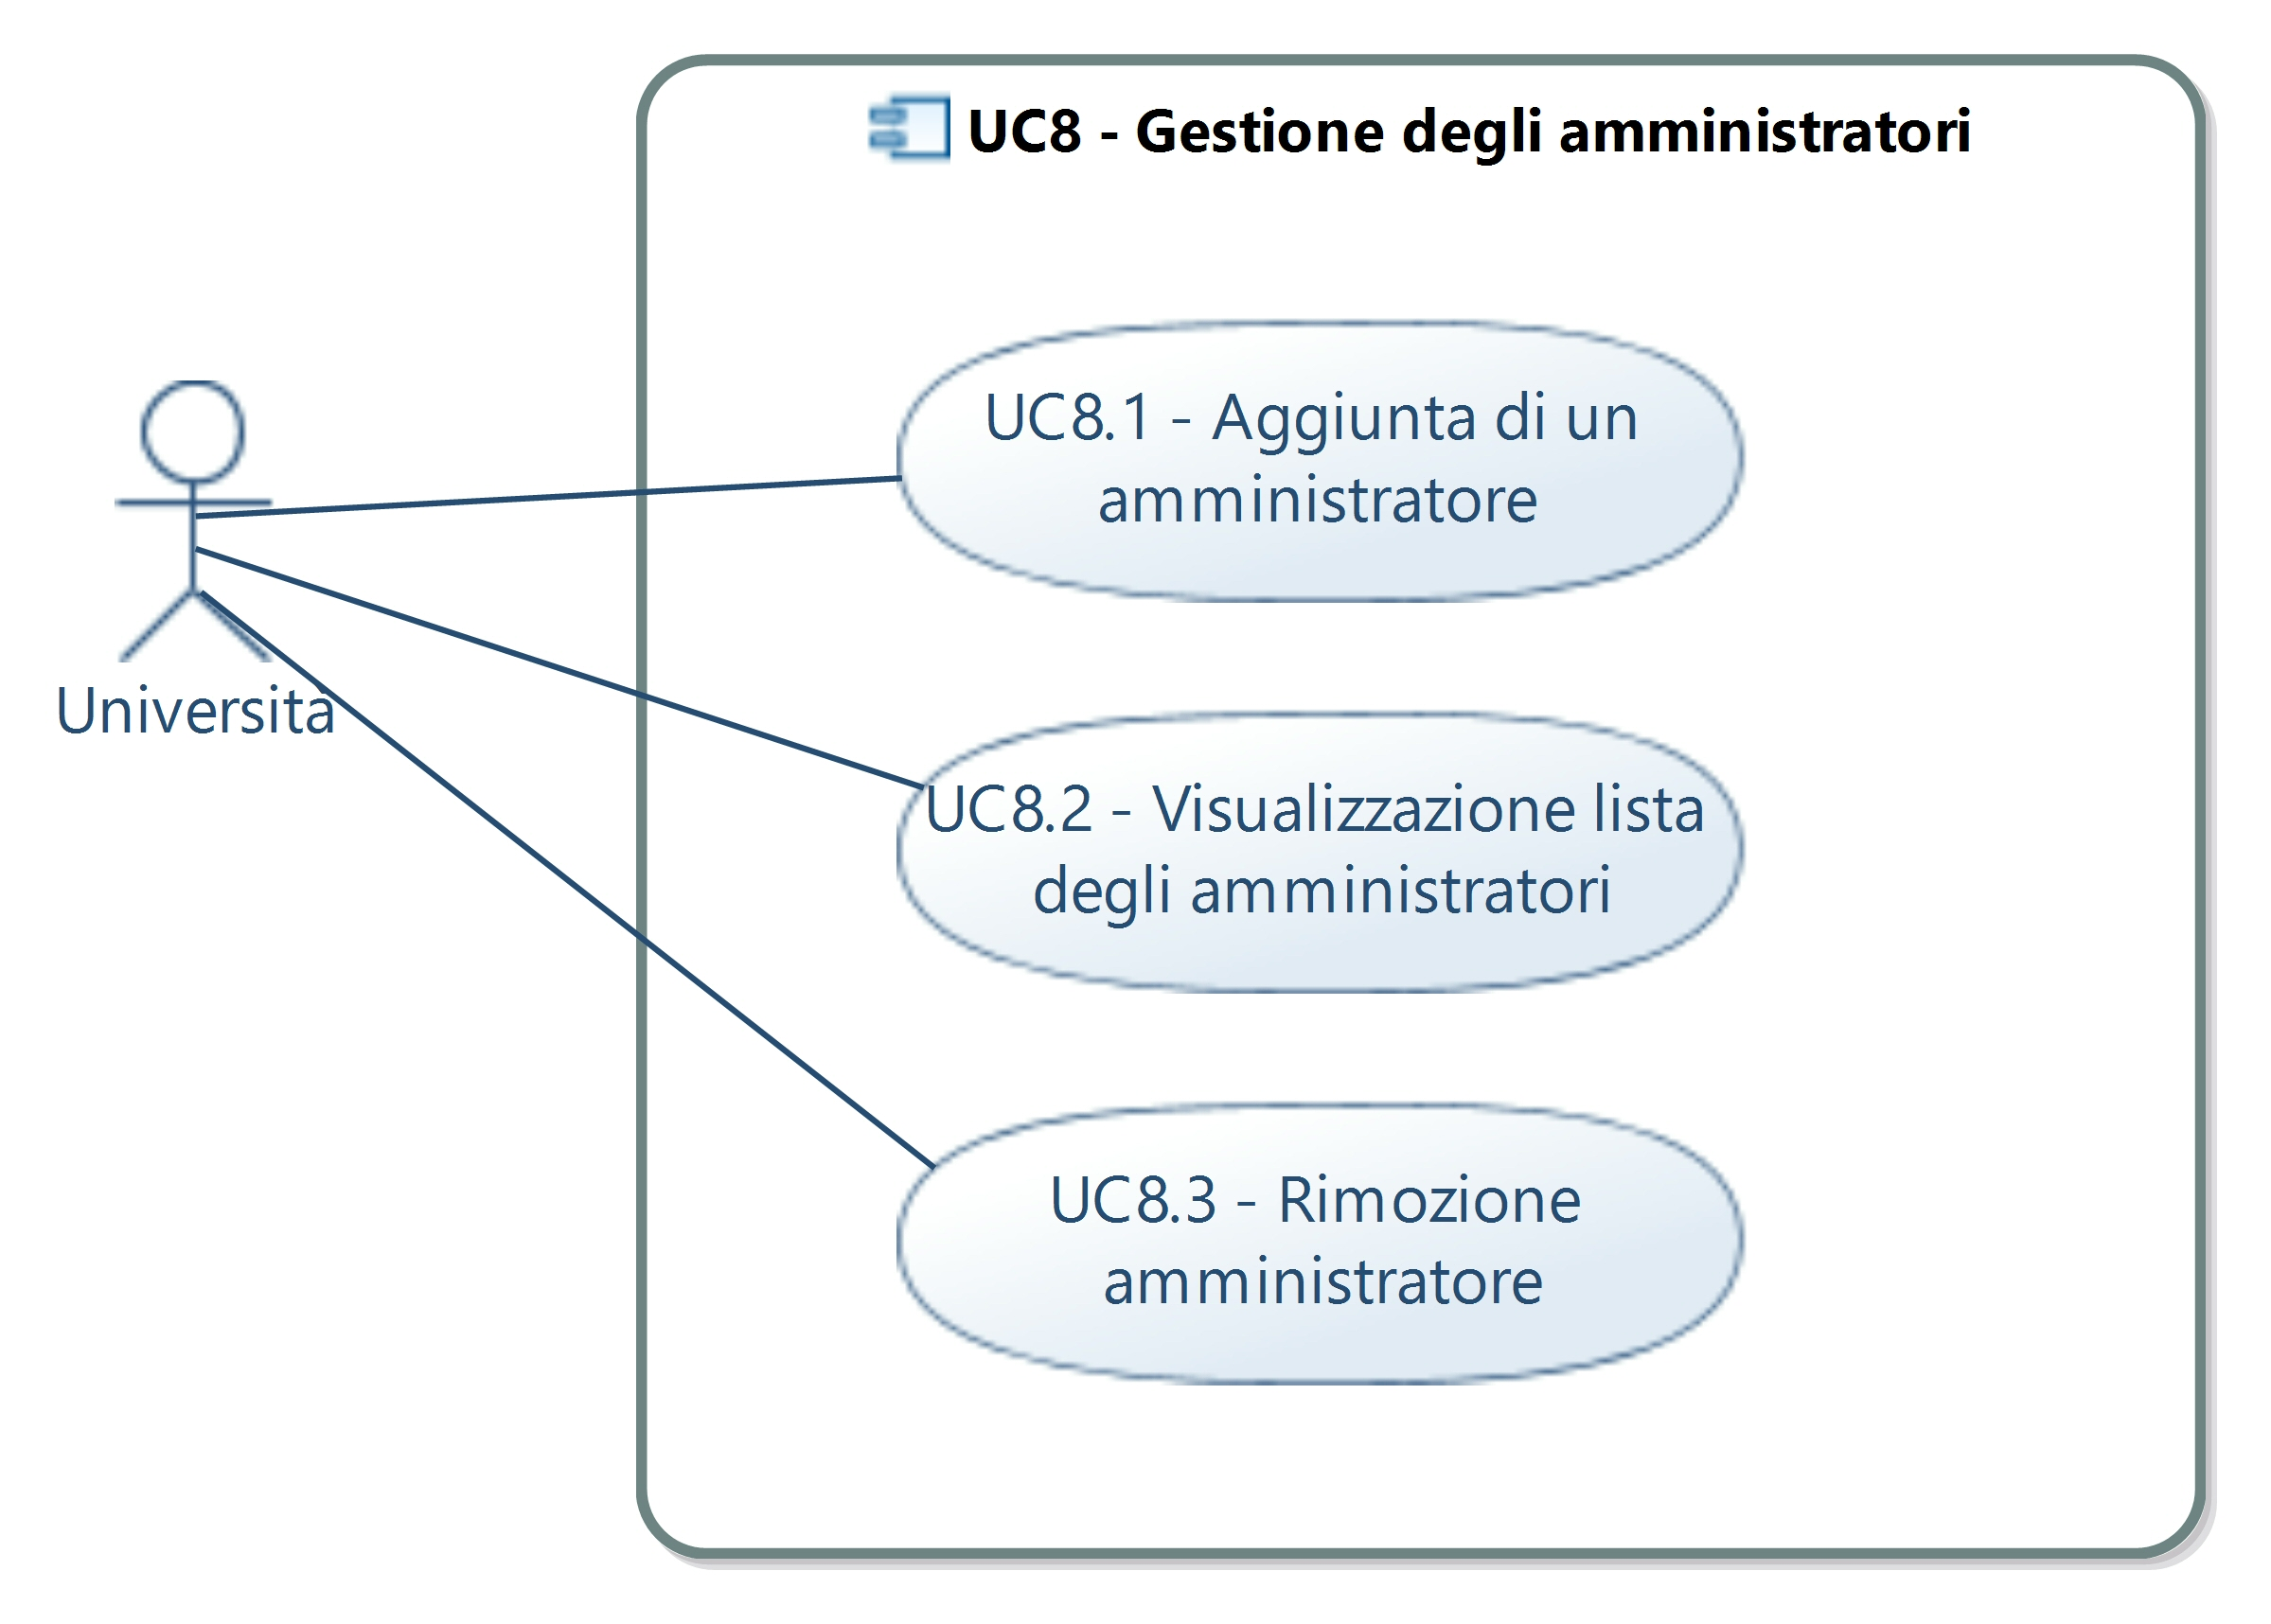
\includegraphics[width=0.8\linewidth]{UC8.jpg}
	\caption{UC8 - Gestione aspetti relativi agli esami}
	\label{fig:UC8 - Gestione aspetti relativi agli esami}
\end{figure}
\subsection{UC8.1 - Visualizzazione lista degli esami}
\begin{itemize}
	\item \textbf{Attori primari:} professore;
	\item \textbf{Scopo e descrizione:} il professore visualizza una lista di tutti gli esami ai quali è assegnato;
	\item \textbf{Scenario principale:} il professore richiede al sistema la lista degli esami di sua competenza per poterla consultare;
	\item \textbf{Precondizione:} il sistema riconosce l'utente nel ruolo del professore e fornisce la lista delle funzionalità alle quali ha accesso relative all'amministrazione degli esami secondo le restrizioni permesse dal suo ruolo; 
	\item \textbf{Postcondizione:} il sistema fornisce al professore la lista degli esami di sua competenza.
\end{itemize}
\begin{figure}[H]
	\centering
	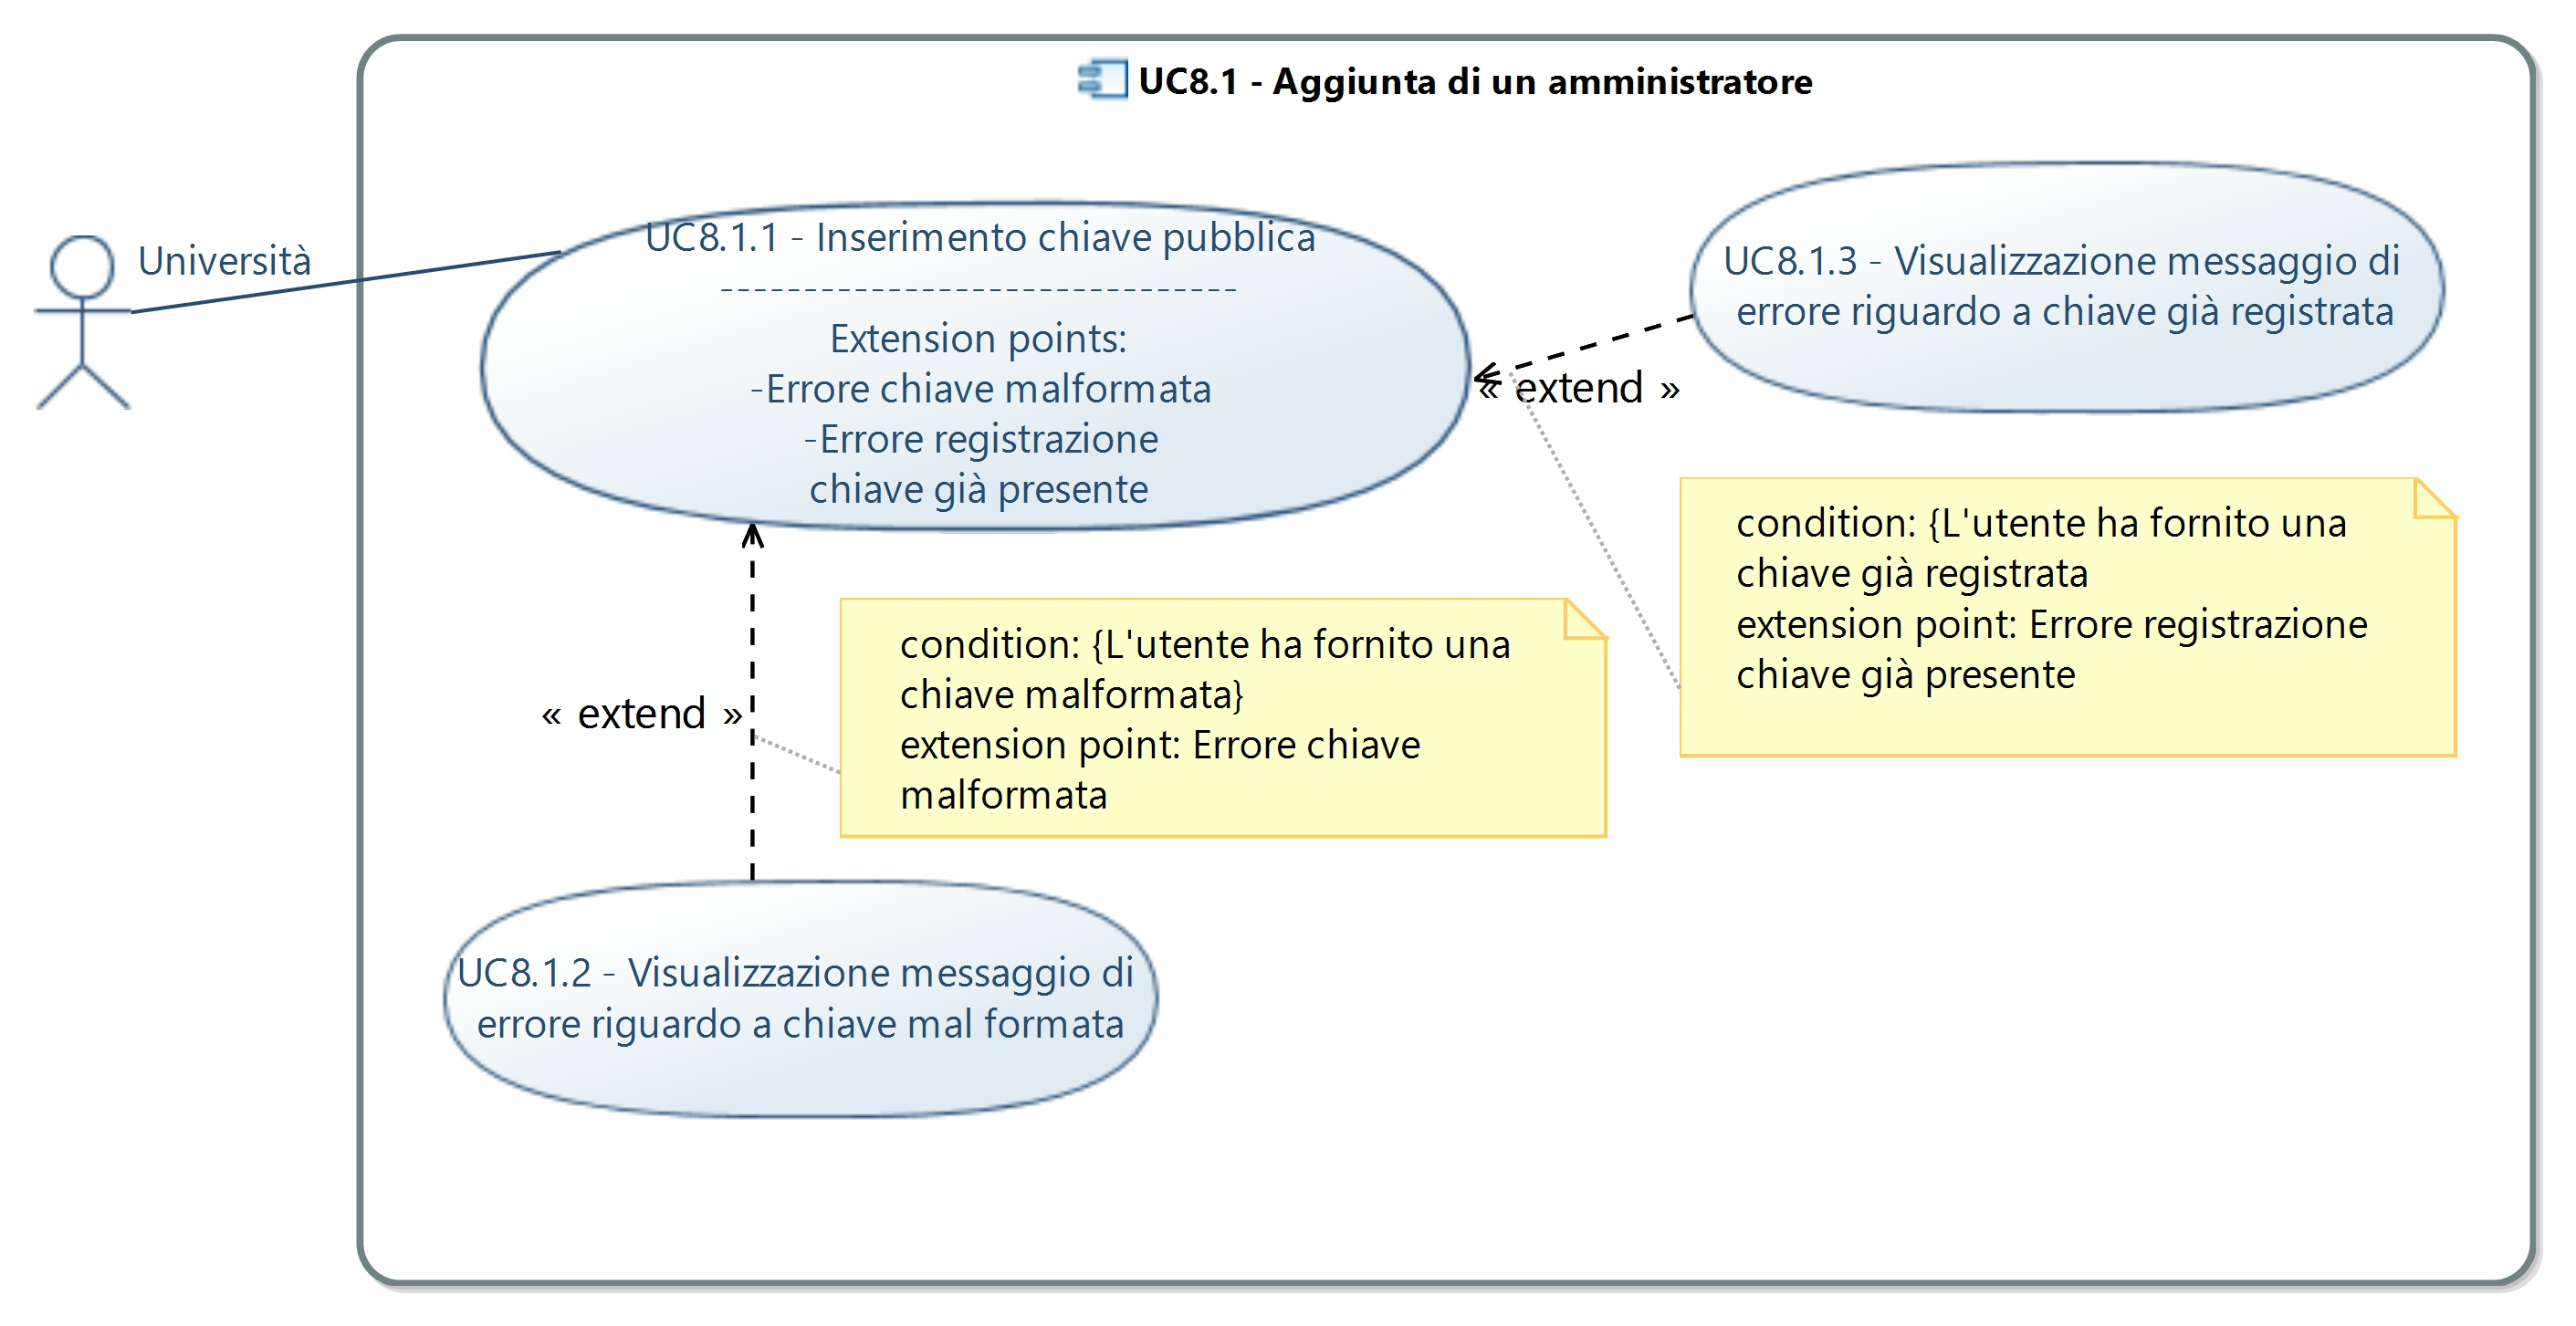
\includegraphics[width=0.7\linewidth]{UC8_1.jpg}
	\caption{UC8.1 - Visualizzazione lista degli esami}
	\label{UC8.1 - Visualizzazione lista degli esami}
\end{figure}
\subsection{UC8.1.1 - Visualizzazione codici degli esami}
\begin{itemize}
	\item \textbf{Attori primari:} professore;
	\item \textbf{Scopo e descrizione:} il professore visualizza per ogni esame il relativo codice;
	\item \textbf{Scenario principale:} il professore richiede al sistema la lista dei codici degli esami di sua competenza per poterla consultare;
	\item \textbf{Precondizione:} il sistema riconosce l'utente nel ruolo del professore, il quale richiede la visualizzazione degli esami di sua competenza;
	\item \textbf{Postcondizione:} il sistema fornisce per ogni esame di competenza del professore il relativo codice.
\end{itemize}
\subsection{UC8.1.2 - Visualizzazione nomi dei corsi degli esami}
\begin{itemize}
	\item \textbf{Attori primari:} professore;
	\item \textbf{Scopo e descrizione:} il professore visualizza per ogni esame il relativo nome del corso di laurea associato;
	\item \textbf{Scenario principale:} il professore richiede al sistema la lista dei nomi dei corsi di laurea degli esami di sua competenza per poterla consultare;
	\item \textbf{Precondizione:} il sistema riconosce l'utente nel ruolo del professore, il quale richiede la visualizzazione degli esami di sua competenza;
	\item \textbf{Postcondizione:} il sistema fornisce per ogni esame di competenza del professore il nome del corso di laurea al quale appartiene.
\end{itemize}

\subsection{UC8.2 - Visualizzazione lista degli studenti}
\begin{itemize}
	\item \textbf{Attori primari:} professore;
	\item \textbf{Scopo e descrizione:} il professore visualizza una lista di tutti gli studenti iscritti a un esame a lui assegnato;
	\item \textbf{Scenario principale:} il professore richiede al sistema la lista degli studenti iscritti a un esami di sua competenza per poterla consultare;
	\item \textbf{Flusso principale degli eventi:}
	\begin{enumerate}
		\item Il professore visualizza la lista degli esami di sua competenza [UC8.1];
		\item Il professore, una volta individuato l'esame al quale è interessato, ne richiede la lista degli studenti registrati [UC8.2].
	\end{enumerate}
	\item \textbf{Precondizione:} il sistema riconosce l'utente nel ruolo del professore e fornisce la lista degli esami di sua competenza [UC8.1]; 
	\item \textbf{Postcondizione:} il sistema fornisce al professore la lista degli studenti iscritti a un dato esame da lui indicatogli.
\end{itemize}
\begin{figure}[H]
	\centering
	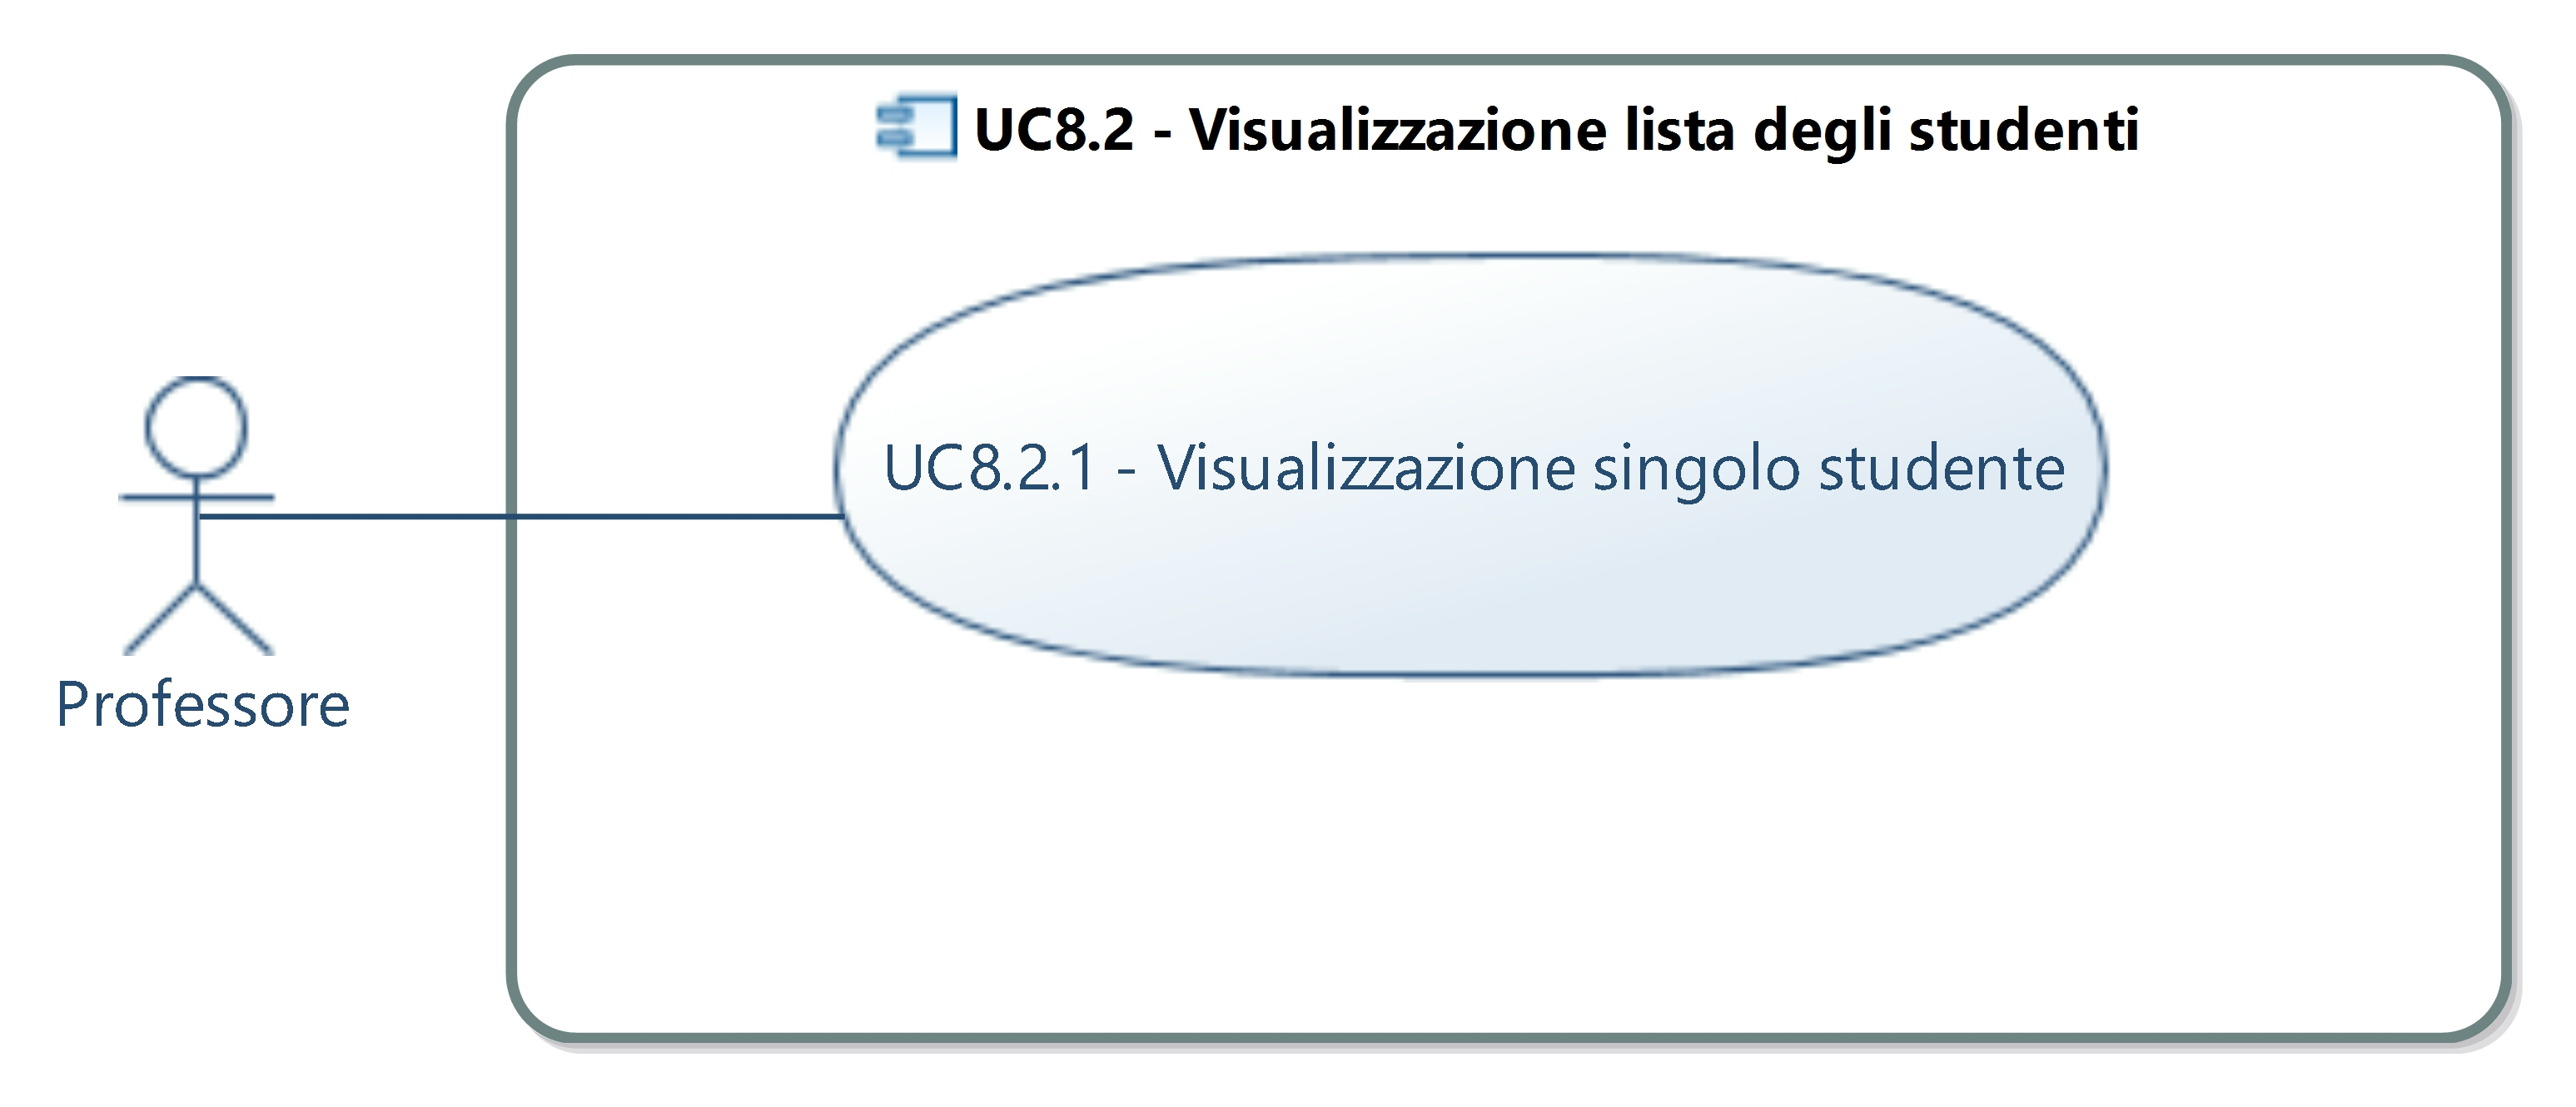
\includegraphics[width=0.7\linewidth]{UC8_2.jpg}
	\caption{UC8.2 - Visualizzazione lista degli studenti}
	\label{UC8.2 - Visualizzazione lista degli studenti}
\end{figure}
\subsection{UC8.2.1 - Visualizzazione indirizzi degli studenti dell'esame}
\begin{itemize}
	\item \textbf{Attori primari:} professore;
	\item \textbf{Scopo e descrizione:} il professore visualizza una lista di tutti gli \citGloss{indirizzi} della rete \citGloss{Ethereum} degli studenti registrati all'esame;
	\item \textbf{Scenario principale:} il professore richiede al sistema una lista di studenti per poterne visualizzare l'\citGloss{indirizzo} ed eventualmente compiere altre operazioni su di essi;
	\item \textbf{Precondizione:} il sistema riconosce l'utente nel ruolo del professore, il quale richiede la visualizzazione degli studenti registrati a un dato esame;
	\item \textbf{Postcondizione:} il sistema fornisce per ogni studente il relativo \citGloss{indirizzo}.
\end{itemize}
\subsection{UC8.2.2 - Visualizzazione nomi degli studenti dell'esame}
\begin{itemize}
	\item \textbf{Attori primari:} professore;
	\item \textbf{Scopo e descrizione:} il professore visualizza una lista di tutti i nomi degli studenti registrati all'esame;
	\item \textbf{Scenario principale:} il professore richiede al sistema una lista di studenti per poterne visualizzare il nome ed eventualmente compiere altre operazioni su di essi;
	\item \textbf{Precondizione:} il sistema riconosce l'utente nel ruolo del professore, il quale richiede la visualizzazione degli studenti registrati a un dato esame;
	\item \textbf{Postcondizione:} il sistema fornisce per ogni studente il relativo nome.
\end{itemize}
\subsection{UC8.2.3 - Visualizzazione cognomi degli studenti dell'esame}
\begin{itemize}
	\item \textbf{Attori primari:} professore;
	\item \textbf{Scopo e descrizione:} il professore visualizza una lista di tutti i cognomi degli studenti registrati all'esame;
	\item \textbf{Scenario principale:} il professore richiede al sistema una lista di studenti per poterne visualizzare il cognome ed eventualmente compiere altre operazioni su di essi;
	\item \textbf{Precondizione:} il sistema riconosce l'utente nel ruolo del professore, il quale richiede la visualizzazione degli studenti registrati a un dato esame;
	\item \textbf{Postcondizione:} il sistema fornisce per ogni studente il relativo cognome.
\end{itemize}

\subsection{UC8.3 - Registrazione valutazione di un esame}
\begin{itemize}
	\item \textbf{Attori primari:} professore;
	\item \textbf{Scopo e descrizione:} il professore inserisce nel sistema una valutazione;
	\item \textbf{Flusso principale degli eventi:}
	\begin{enumerate}
		\item Il professore visualizza la lista degli esami di sua competenza [UC8.1];
		\item Il professore, una volta individuato l'esame al quale è interessato, ne richiede la lista degli studenti registrati [UC8.2];
		\item Il professore consulta la lista degli studenti e individua la persona alla quale deve inserire la valutazione [UC8.2];
		\item Il professore inserisce la valutazione allo studente [UC8.3].
	\end{enumerate}
	\item \textbf{Precondizione:} il sistema fornisce al professore la lista degli esami di sua competenza [UC8.1] e, dopo che l'utente ne ha indicato uno, fornisce la lista degli studenti registrati a esso [UC8.2];
	\item \textbf{Postcondizione:} il sistema fornisce gli elementi necessari per registrare l'esame sulla \citGloss{blockchain}.
\end{itemize}
\begin{figure}[H]
	\centering
	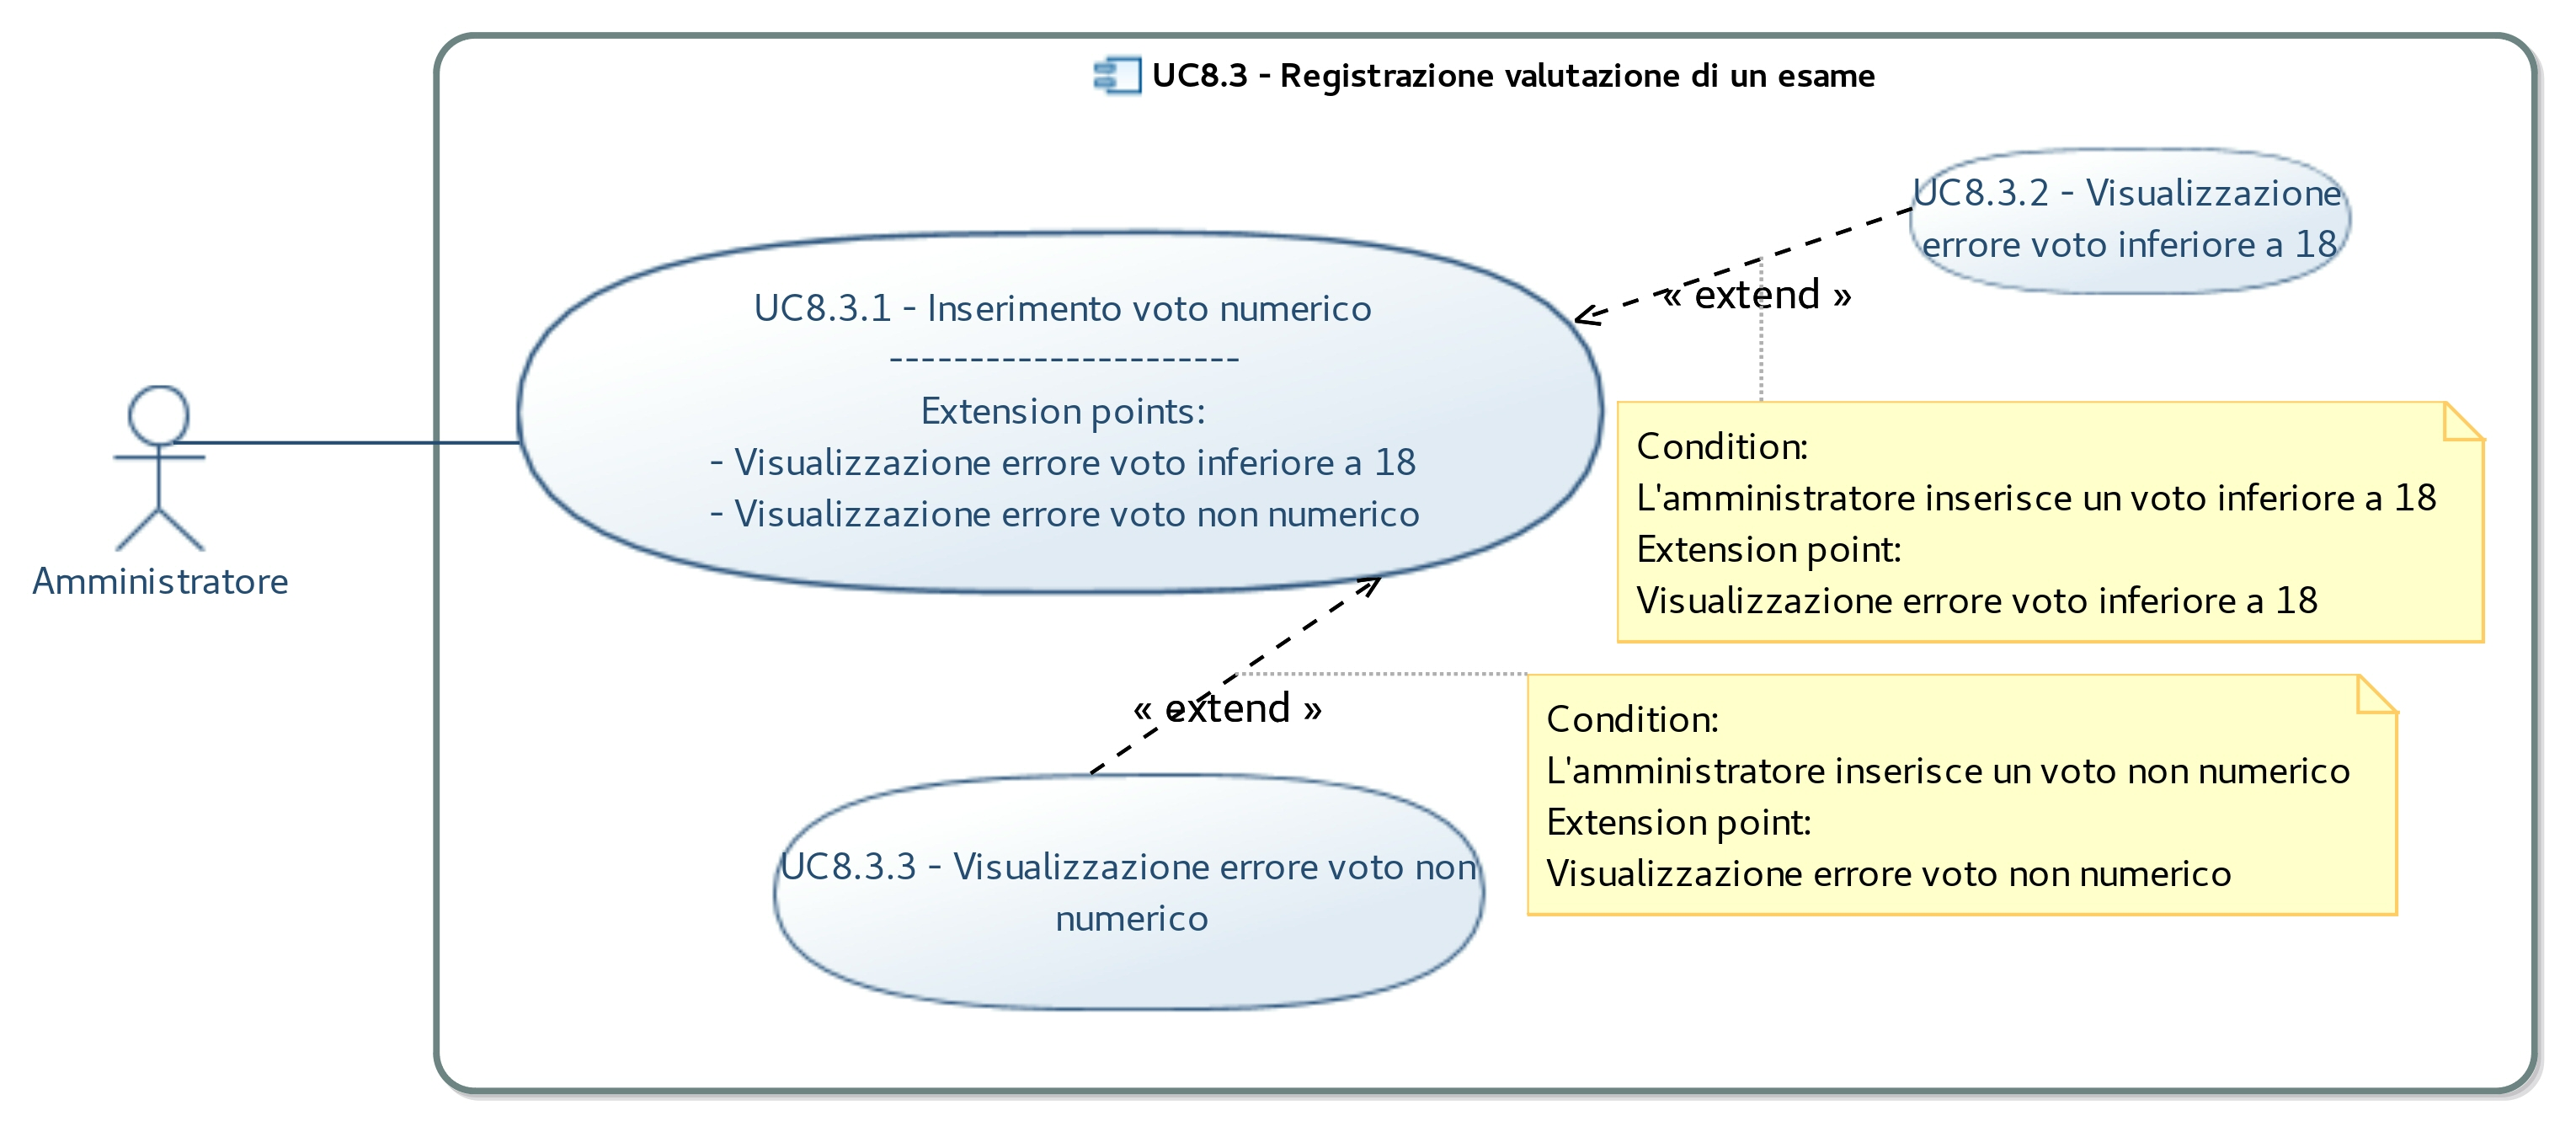
\includegraphics[width=0.7\linewidth]{UC8_3.jpg}
	\caption{UC8.3 - Registrazione valutazione di un esame}
	\label{UC8.3 - Registrazione valutazione di un esame}
\end{figure}
\subsection{UC8.3.1 - Inserimento voto numerico}
\begin{itemize}
	\item \textbf{Attori primari:} professore;
	\item \textbf{Scopo e descrizione:} il professore inserisce la valutazione numerica relativa all'esame;
	\item \textbf{Scenario principale:} il professore riempie il campo dati relativo alla valutazione con un voto superiore a 17;
	\item \textbf{Estensioni:}
	\begin{itemize}
		\item Se il professore inserisce un voto inferiore a 18 viene avvisato con un messaggio d'errore a riguardo [UC8.3.2];
		\item Se il professore inserisce un voto non numerico viene avvisato con un errore a riguardo [UC8.3.3].
	\end{itemize}
	\item \textbf{Precondizione:} Il sistema fornisce al professore un campo dati per inserire il voto; 
	\item \textbf{Postcondizione:} Il sistema riceve il voto e lo inserisce all'interno della \citGloss{blockchain}.
\end{itemize}
\subsection{UC8.3.2 - Visualizzazione errore voto inferiore a 18}
\begin{itemize}
	\item \textbf{Attori primari:} professore;
	\item \textbf{Scopo e descrizione:} il professore viene avvisato che ha inserito un voto inferiore a 18;
	\item \textbf{Scenario principale:} il professore visualizza una schermata d'errore relativa all'inserimento del voto;
	\item \textbf{Precondizione:} il sistema riceve un voto inferiore a 18; 
	\item \textbf{Postcondizione:} il sistema mostra una schermata d'errore per avvisare il professore.
\end{itemize}
\subsection{UC8.3.3 - Visualizzazione errore voto non numerico}
\begin{itemize}
	\item \textbf{Attori primari:} professore;
	\item \textbf{Scopo e descrizione:} il professore viene avvisato che ha inserito un voto non numerico;
	\item \textbf{Scenario principale:} il professore visualizza una schermata d'errore relativa all'inserimento del voto;
	\item \textbf{Precondizione:} il sistema riceve un voto non numerico; 
	\item \textbf{Postcondizione:} il sistema mostra una schermata d'errore per avvisare il professore.
\end{itemize}
\subsection{UC9 - Gestione aspetti relativi allo studente}
\begin{itemize}
	\item \textbf{Attori primari:} studente;
	\item \textbf{Attori secondari:} \citGloss{MetaMask};
	\item \textbf{Scopo e descrizione:} l'utente è già riconosciuto dal sistema come studente e sceglie di utilizzare una funzionalità messa a sua disposizione da parte del sistema;
	\item \textbf{Precondizione:} il sistema riconosce l'utente nel ruolo di studente e mette a disposizione una serie di operazioni atte alla gestione degli aspetti relativi al perseguimento della laurea;
	\item \textbf{Postcondizione:} il sistema effettua le operazioni richieste riguardanti il perseguimento della laurea.
\end{itemize}
\begin{figure}[H]
	\centering
	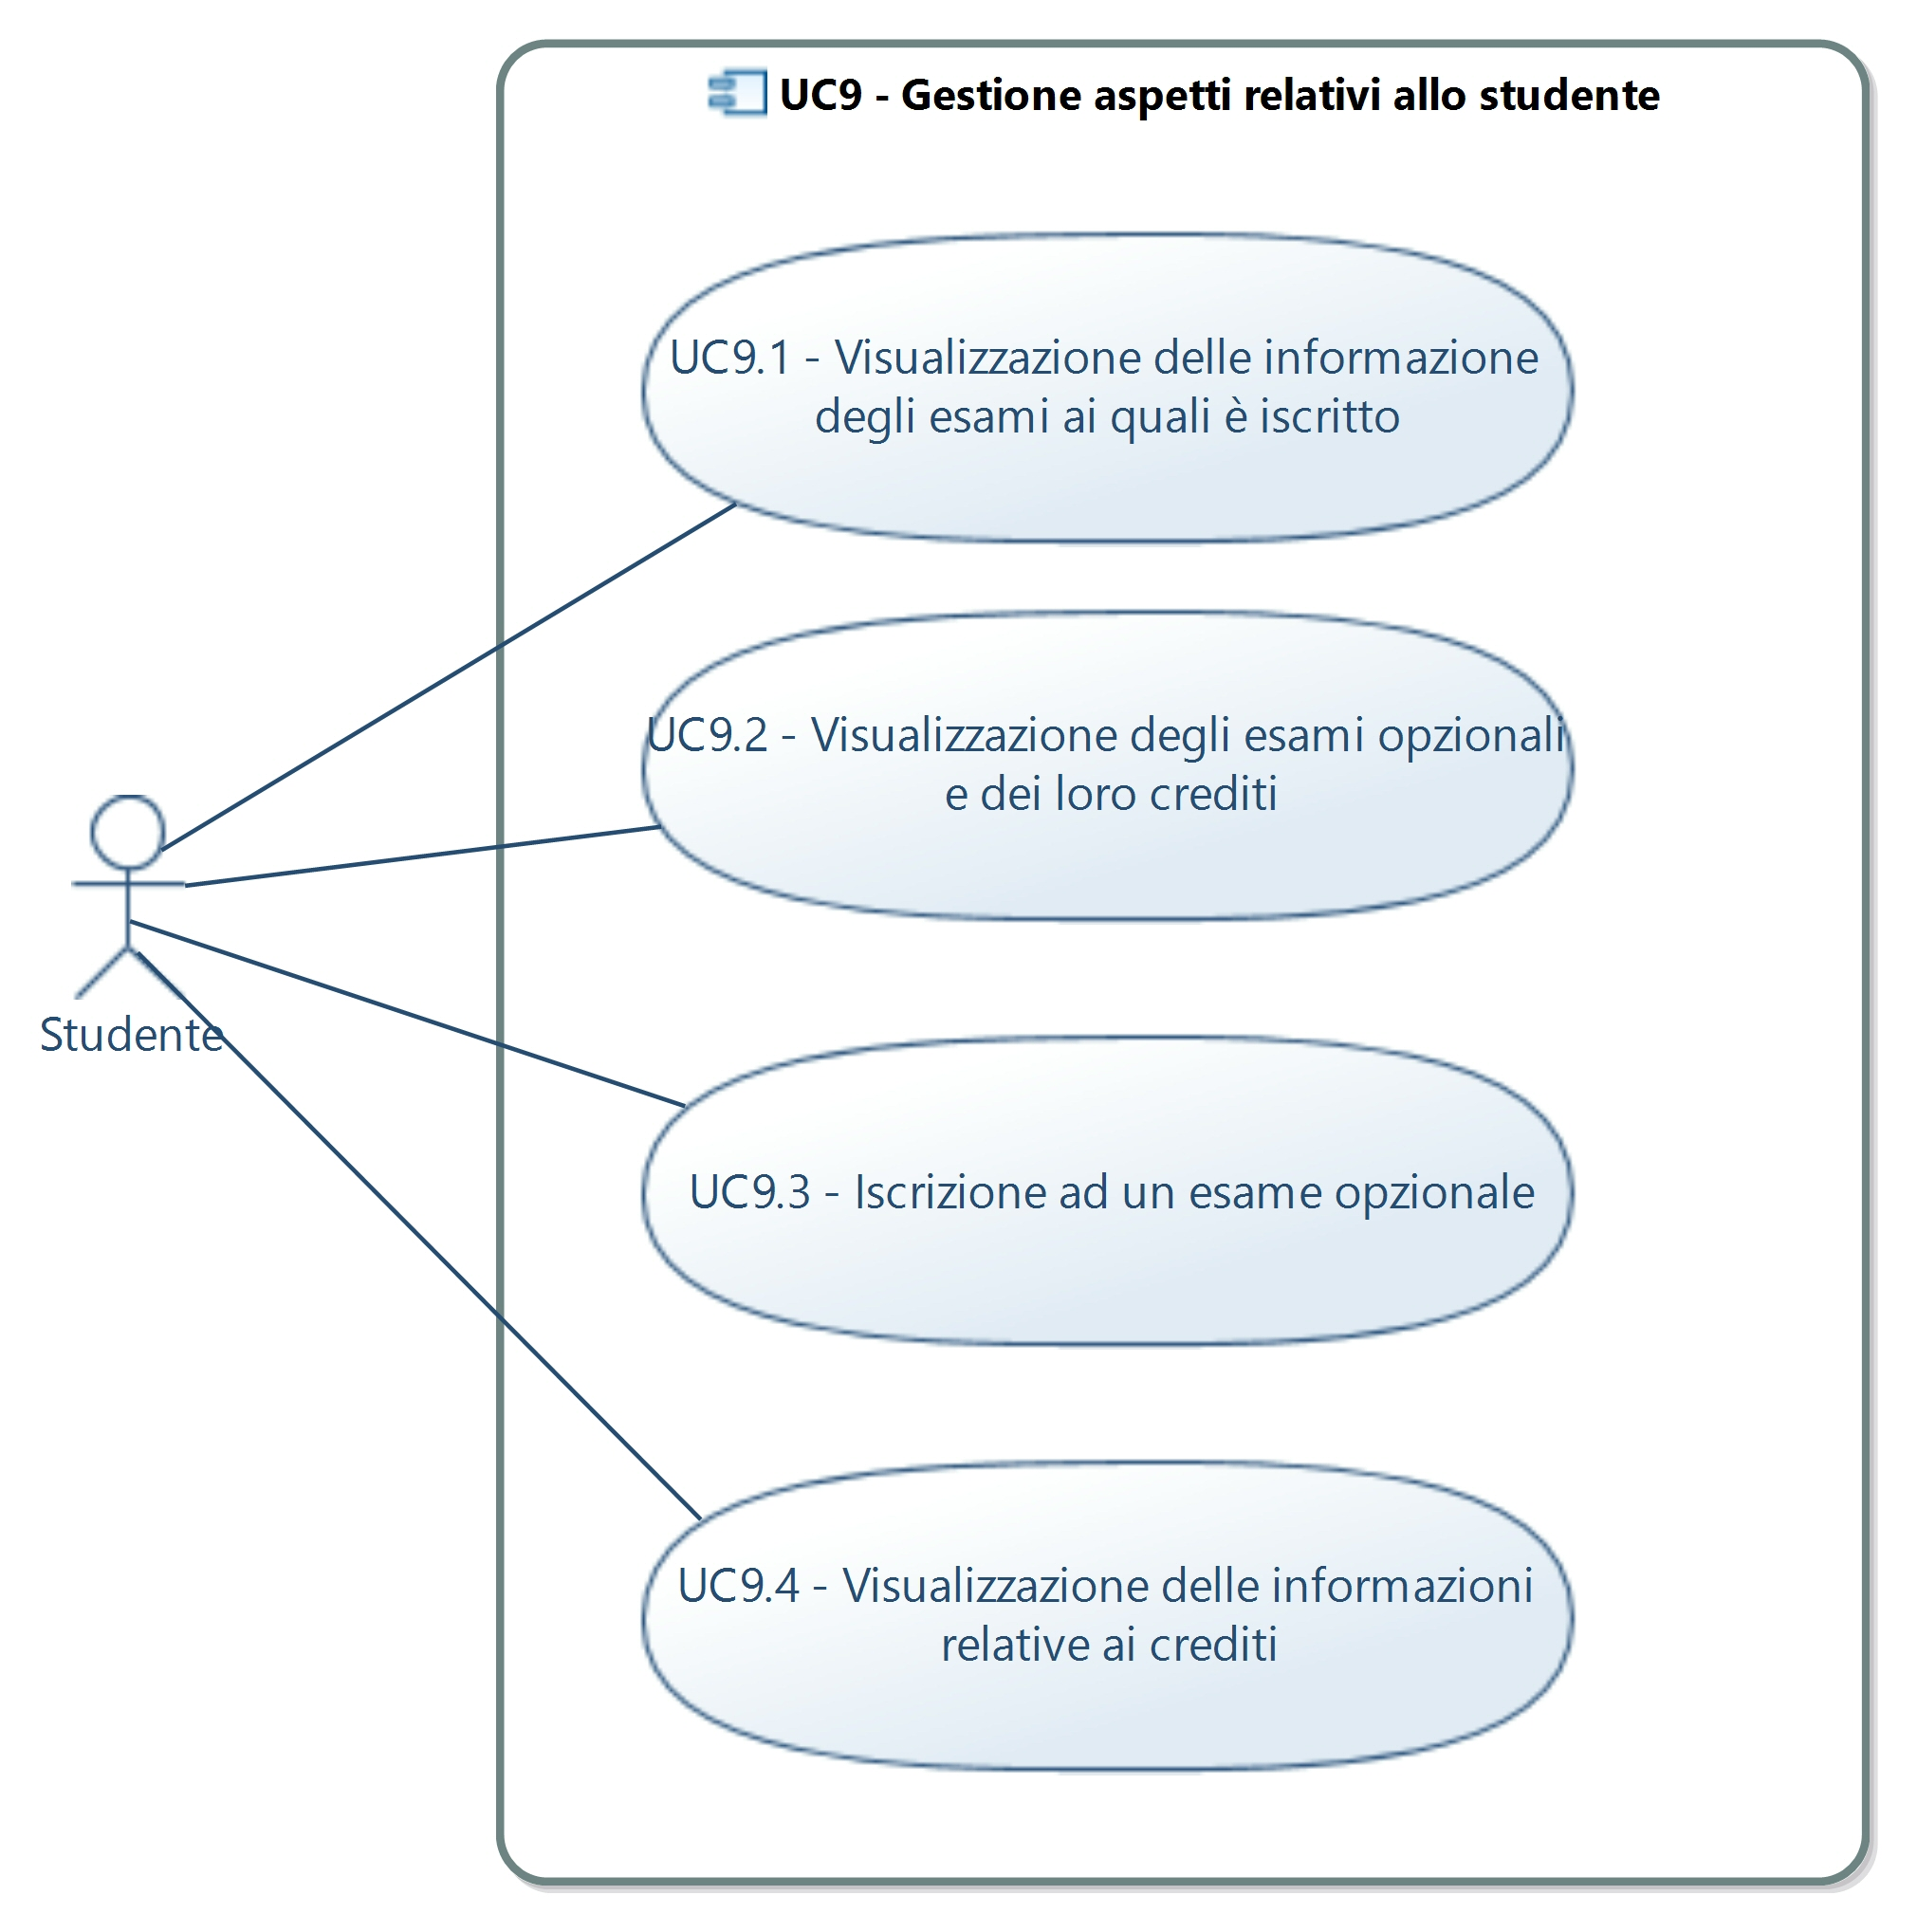
\includegraphics[width=0.8\linewidth]{UC9.jpg}
	\caption{UC9 - Gestione aspetti relativi allo studente}
	\label{fig:UC9 - Gestione aspetti relativi allo studente}
\end{figure}

\subsection{UC9.1 - Visualizzazione delle informazione degli esami ai quali è iscritto}
\begin{itemize}
	\item \textbf{Attori primari:} studente;
	\item \textbf{Scopo e descrizione:} lo studente visualizza una lista di tutti gli esami ai quali è iscritto indicati dal nome;
	\item \textbf{Scenario principale:} lo studente richiede al sistema la lista degli esami ai quali è iscritto per poterla consultare;
	\item \textbf{Precondizione:} il sistema riconosce l'utente nel ruolo di studente e fornisce la lista delle funzionalità alle quali ha accesso relative alla gestione degli esami secondo le restrizioni permesse dal suo ruolo; 
	\item \textbf{Postcondizione:} il sistema fornisce allo studente la lista degli esami al quale è iscritto.
\end{itemize}

\begin{figure}[H]
	\centering
	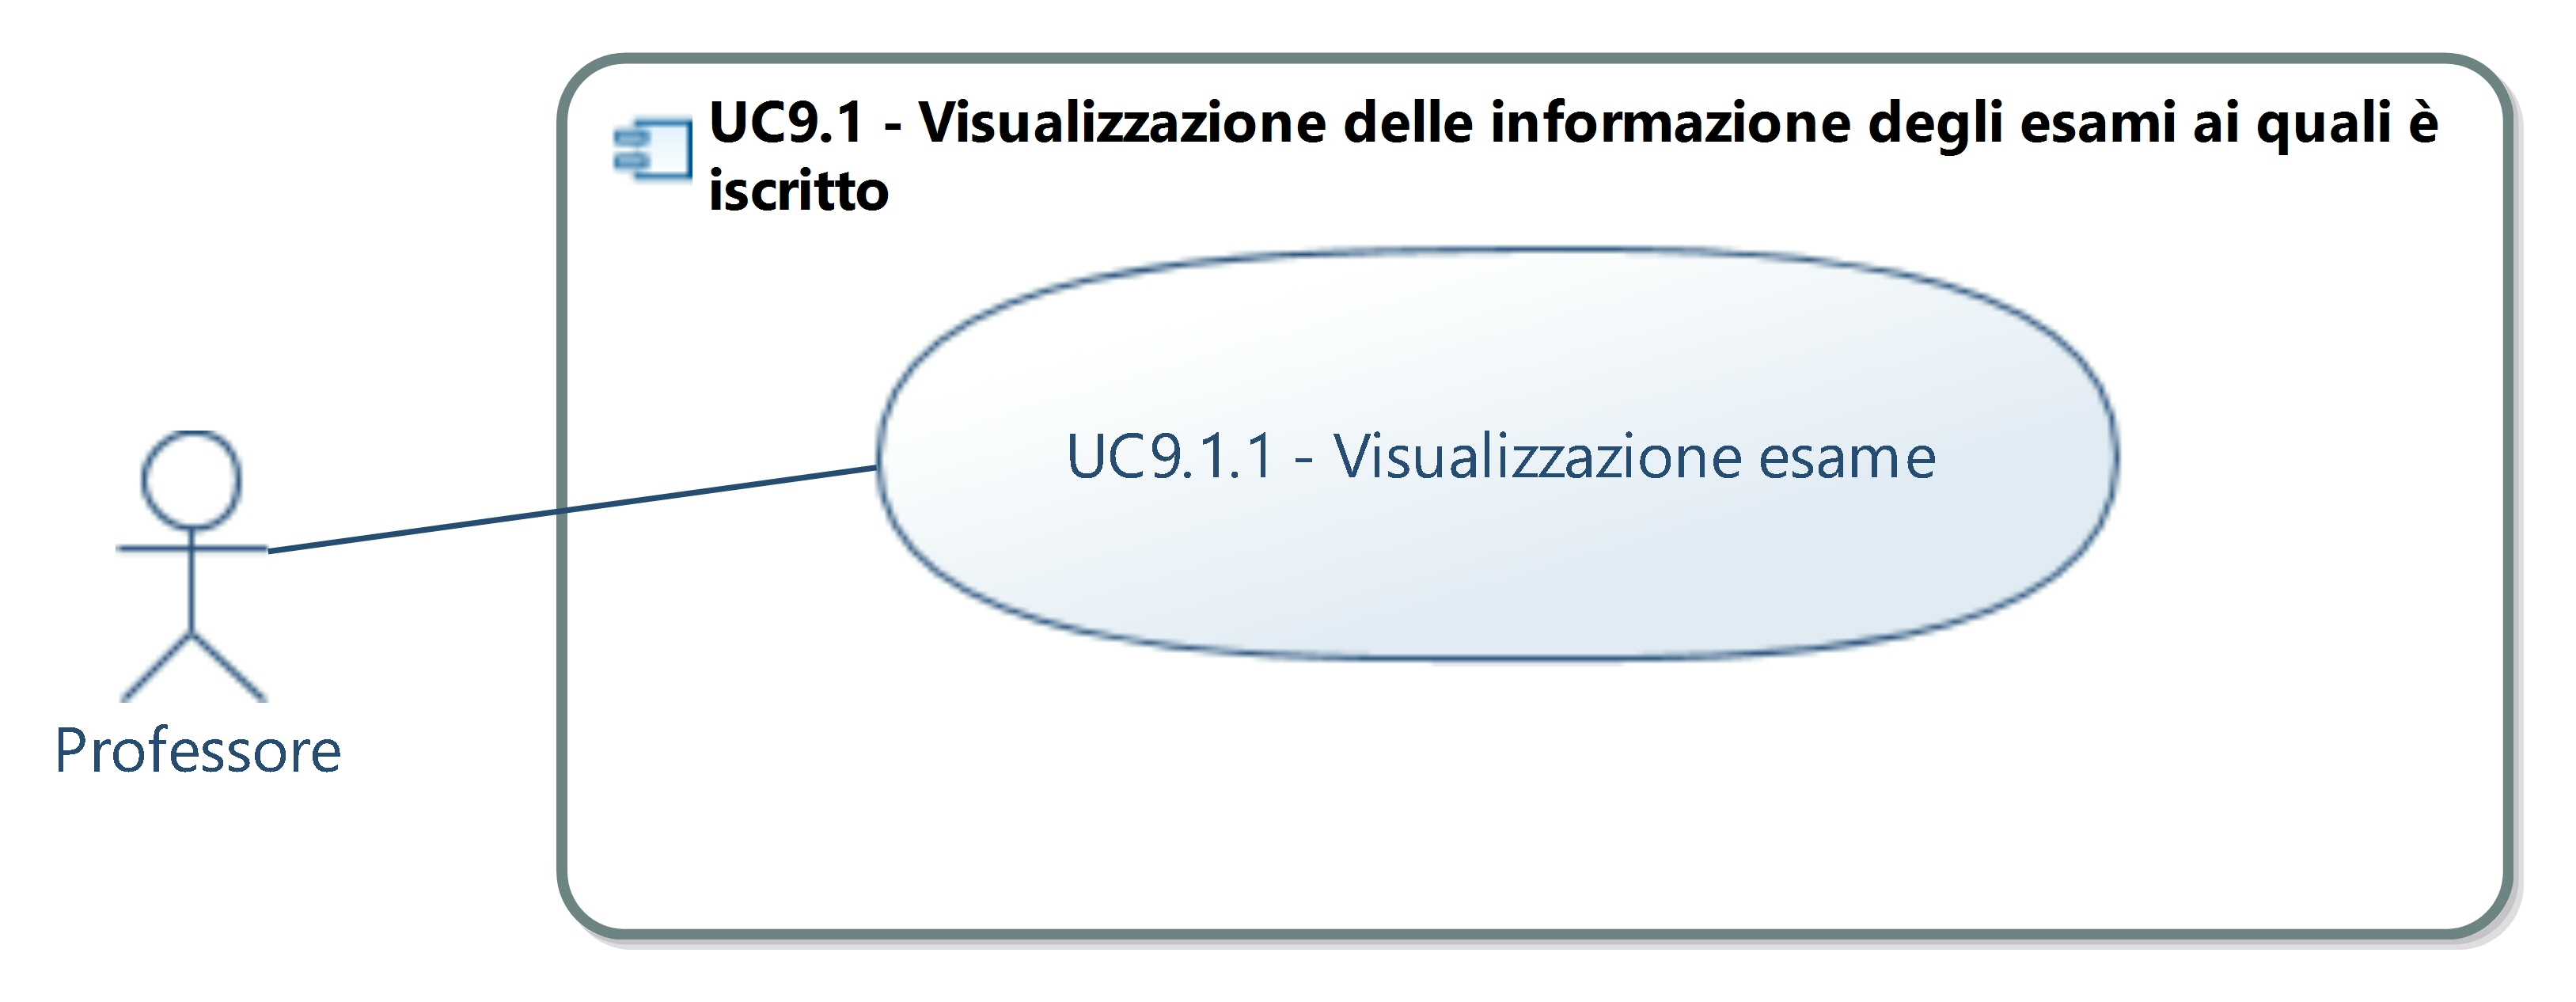
\includegraphics[width=1.0\linewidth]{UC9_1.jpg}
	\caption{UC9.1 - Visualizzazione delle informazione degli esami ai quali è iscritto}
	\label{fig:UC9.1 - Visualizzazione delle informazione degli esami ai quali 'e iscritto}
\end{figure}

\subsection{UC9.1.1 - Visualizzazione dei crediti degli esami ai quali è iscritto}
\begin{itemize}
	\item \textbf{Attori primari:} studente;
	\item \textbf{Scopo e descrizione:} lo studente visualizza il numero di crediti per ogni esame al quale è iscritto;
	\item \textbf{Scenario principale:} lo studente richiede al sistema il numero di crediti degli esami ai quali è iscritto per consultarli;
	\item \textbf{Precondizione:} il sistema riconosce l'utente nel ruolo di studente, il quale richiede la lista degli esami ai quali risulta iscritto; 
	\item \textbf{Postcondizione:} il sistema fornisce, per ogni esame al quale lo studente risulta iscritto, il relativo numero di crediti.
\end{itemize}

\subsection{UC9.1.2 - Visualizzazione della obbligatorietà degli esami ai quali è iscritto}
\begin{itemize}
	\item \textbf{Attori primari:} studente;
	\item \textbf{Scopo e descrizione:} lo studente visualizza l'obbligatorietà di per ogni esame al quale è iscritto;
	\item \textbf{Scenario principale:} lo studente richiede al sistema l'obbligatorietà degli esami ai quali è iscritto;
	\item \textbf{Precondizione:} il sistema riconosce l'utente nel ruolo di studente, il quale richiede la lista degli esami ai quali risulta iscritto; 
	\item \textbf{Postcondizione:} il sistema fornisce, per ogni esame al quale lo studente risulta iscritto, la relativa obbligatorietà.
\end{itemize}

\subsection{UC9.1.3 - Visualizzazione delle valutazioni degli esami ai quali è iscritto}
\begin{itemize}
	\item \textbf{Attori primari:} studente;
	\item \textbf{Scopo e descrizione:} lo studente visualizza la valutazione, in formato numerico con l'indicazione di averlo superato se il voto è superiore a 18, per ogni esame al quale è iscritto;
	\item \textbf{Scenario principale:} lo studente richiede al sistema le informazioni riguardanti le valutazioni degli esami ai quali è iscritto per consultarle;
	\item \textbf{Precondizione:} il sistema riconosce l'utente nel ruolo di studente, il quale richiede la lista degli esami ai quali risulta iscritto; 
	\item \textbf{Postcondizione:} il sistema fornisce, per ogni esame al quale lo studente risulta iscritto, la relativa valutazione, ove presente.
\end{itemize}

\subsection{UC9.2 - Visualizzazione degli esami opzionali e dei loro crediti}
\begin{itemize}
	\item \textbf{Attori primari:} studente;
	\item \textbf{Scopo e descrizione:} lo studente visualizza una lista di tutti gli esami opzionali del suo corso, con indicati nomi e crediti, ai quali ha possibilità di iscriversi;
	\item \textbf{Scenario principale:} lo studente richiede al sistema la lista di tutti gli esami opzionali ai quali ha possibilità di iscriversi per poterla consultare;
	\item \textbf{Precondizione:} il sistema riconosce l'utente nel ruolo di studente e fornisce la lista delle funzionalità alle quali ha accesso relative alla gestione degli esami secondo le restrizioni permesse dal suo ruolo; 
\item \textbf{Postcondizione:} il sistema fornisce allo studente la lista degli esami opzionali ai quali può iscriversi.
\end{itemize}

\subsection{UC9.3 - Iscrizione a un esame opzionale}
\begin{itemize}
	\item \textbf{Attori primari:} studente;
	\item \textbf{Scopo e descrizione:} lo studente si iscrive a un determinato esame opzionale;
	\item \textbf{Flusso principale degli eventi:}
	\begin{enumerate}
		\item Lo studente visualizza la lista degli esami opzionali [UC9.2];
		\item Lo studente individua l'esame al quale è interessato iscriversi;
		\item Lo studente compie l'operazione di iscrizione.
	\end{enumerate}
	\item \textbf{Postcondizione:} il sistema fornisce allo studente la lista degli esami opzionali ai quali può iscriversi e quest'ultimo ne individua uno di suo interesse;
	\item \textbf{Postcondizione:} il sistema iscrive l'utente all'esame opzionale da lui scelto.
\end{itemize}

\subsection{UC9.4 - Visualizzazione delle informazioni relative ai crediti}
\begin{itemize}
	\item \textbf{Attori primari:} studente;
	\item \textbf{Scopo e descrizione:} lo studente visualizza un riepilogo del numero dei crediti che possiede e dell'obiettivo per poter conseguire la laurea;
	\item \textbf{Scenario principale:} lo studente richiede al sistema le informazioni riguardanti i suoi crediti;
	\item \textbf{Precondizione:} il sistema riconosce l'utente nel ruolo di studente e fornisce la lista delle funzionalità alle quali ha accesso relative alla gestione degli esami secondo le restrizioni permesse dal suo ruolo; 
	\item \textbf{Postcondizione:} il sistema fornisce allo studente delle informazioni riguardanti la sua attuale situazione universitaria.
\end{itemize}
\begin{figure}[H]
	\centering
	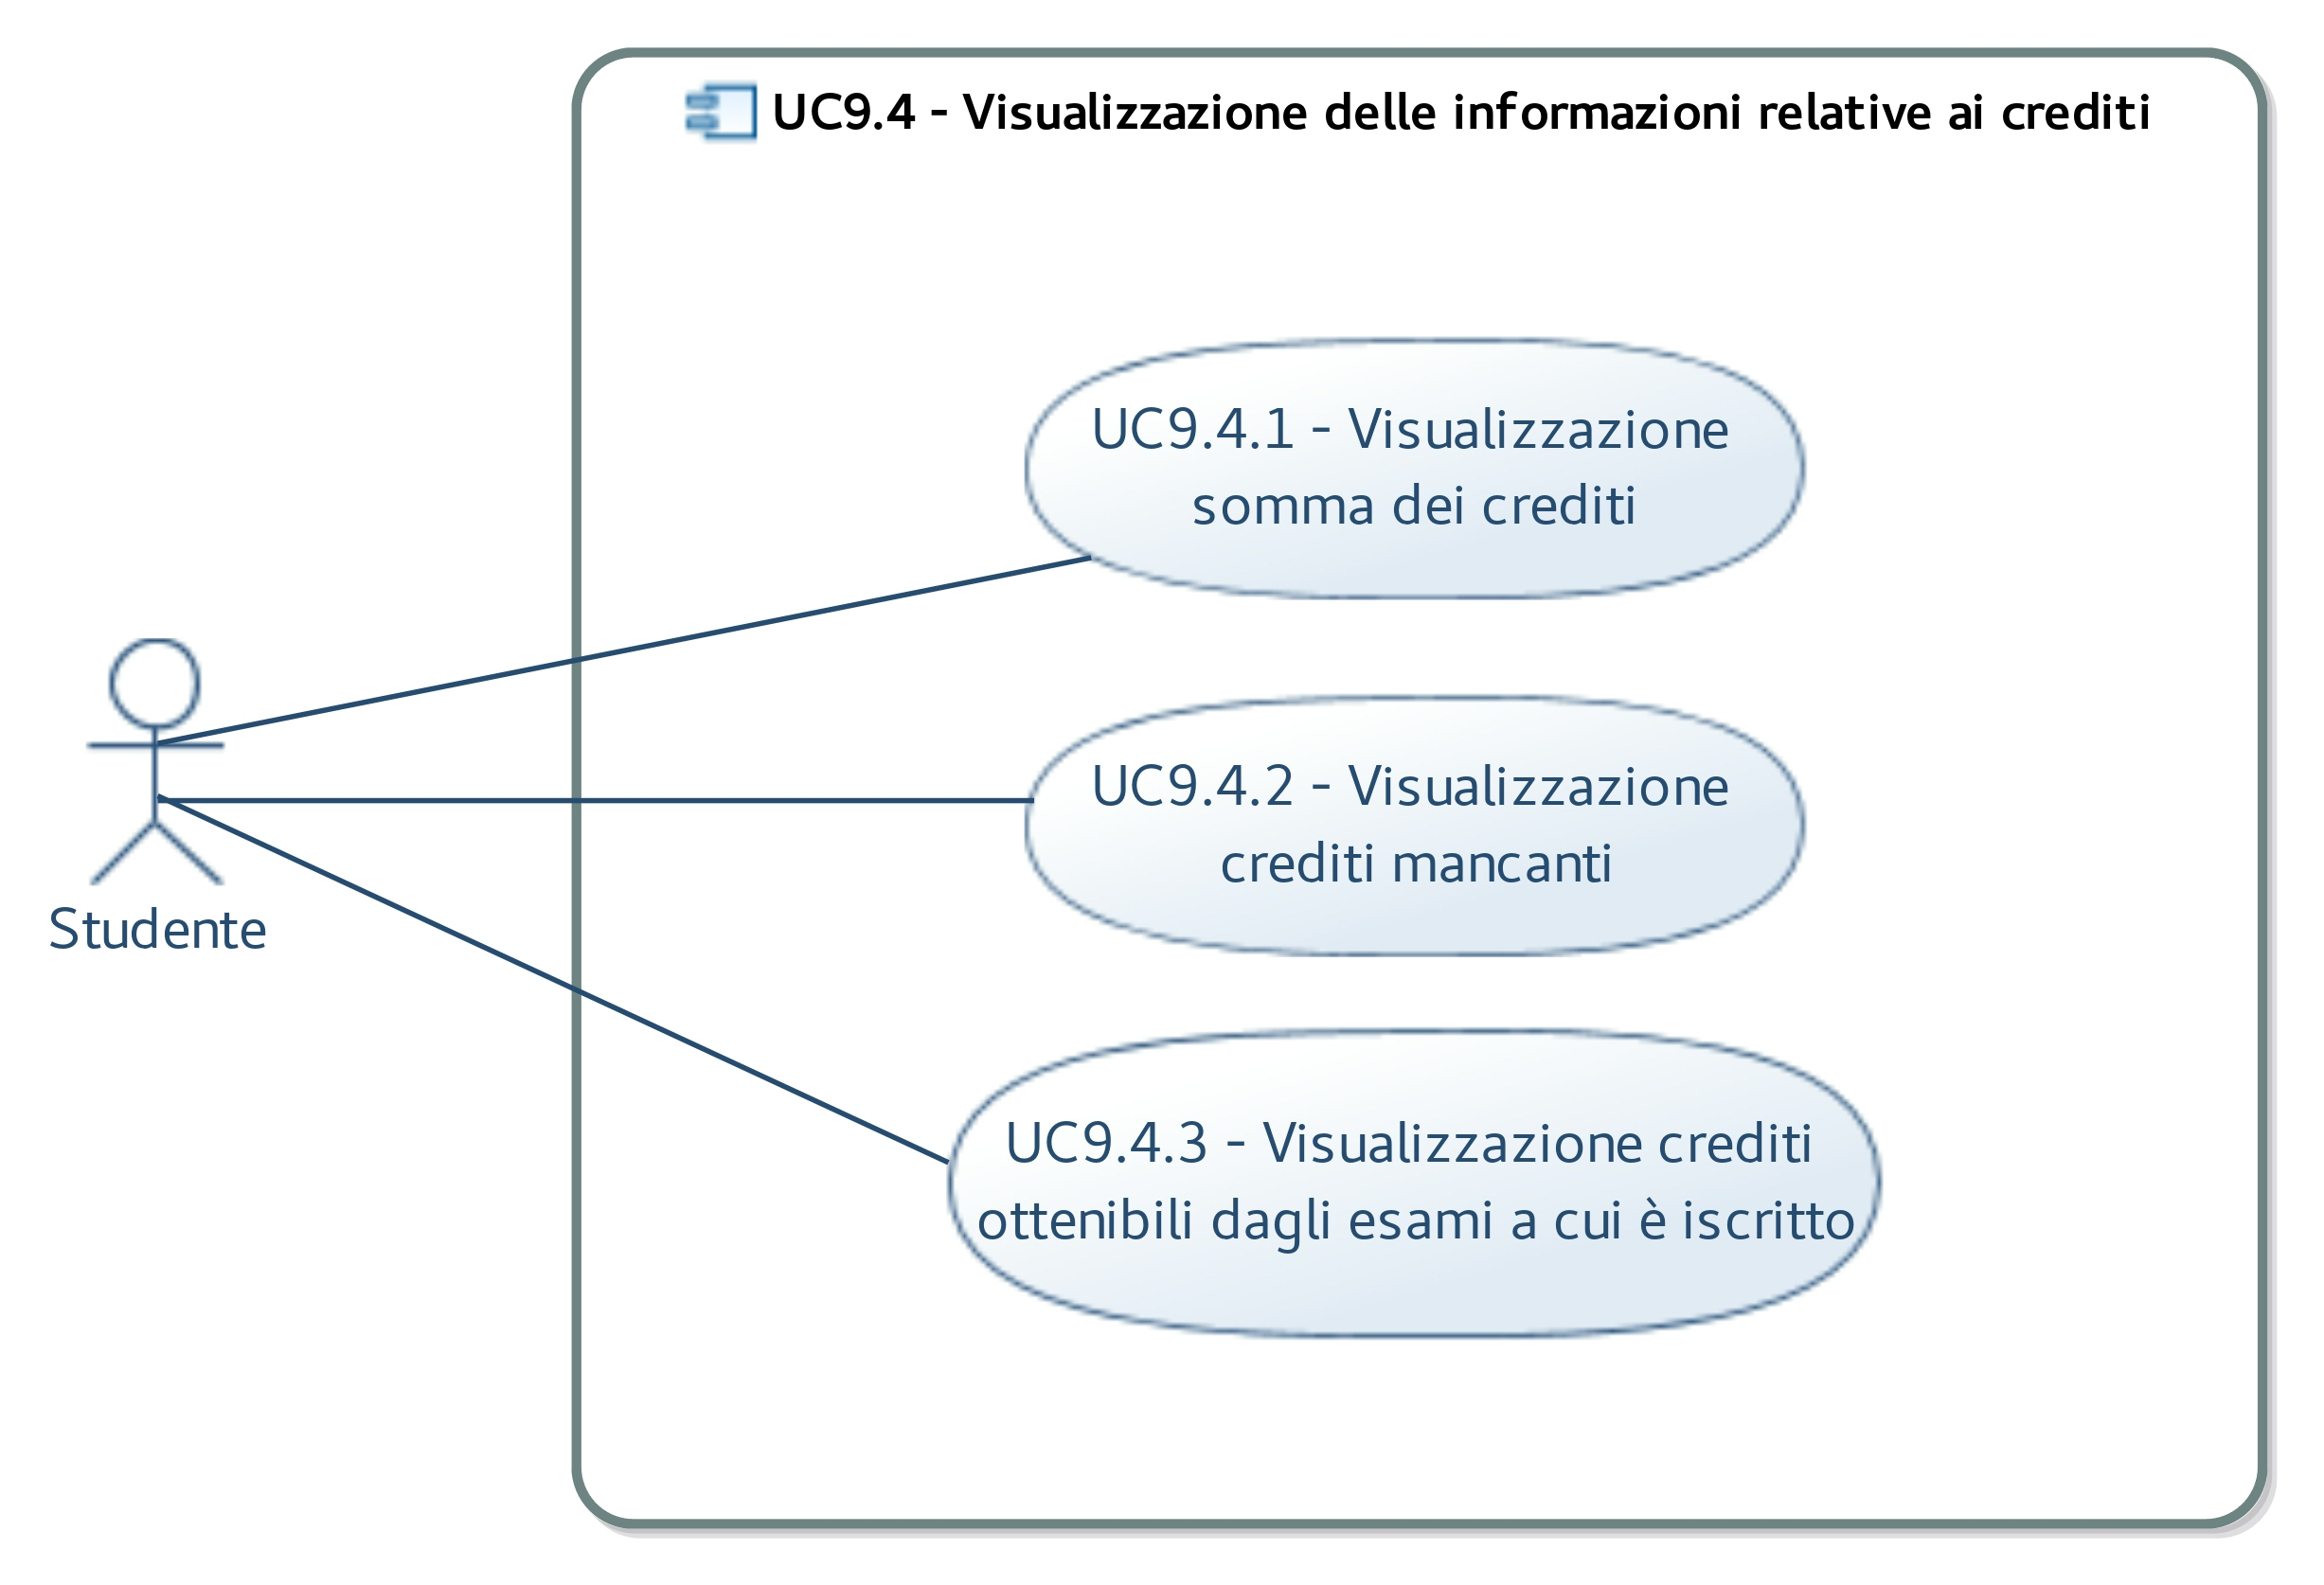
\includegraphics[width=1.0\linewidth]{UC9_4.jpg}
	\caption{UC9.4 - Visualizzazione delle informazioni relative ai crediti}
	\label{fig:UC9.4 - Visualizzazione delle informazioni relative ai crediti}
\end{figure}
\subsection{UC9.4.1 - Visualizzazione somma dei crediti}
\begin{itemize}
	\item \textbf{Attori primari:} studente;
	\item \textbf{Scopo e descrizione:} lo studente visualizza il numero di crediti totalizzati nel suo percorso di studi;
	\item \textbf{Scenario principale:} lo studente richiede al sistema la somma totale dei crediti a lui assegnati;
	\item \textbf{Precondizione:} il sistema mostra allo studente il riepilogo del suo percorso accademico;
	\item \textbf{Postcondizione:} il sistema fornisce allo studente le informazioni relative al numero di crediti realizzati.
\end{itemize}
\subsection{UC9.4.2 - Visualizzazione crediti mancanti}
\begin{itemize}
	\item \textbf{Attori primari:} studente;
	\item \textbf{Scopo e descrizione:} lo studente visualizza il numero di crediti mancanti per completare il suo percorso di studi;
	\item \textbf{Scenario principale:} lo studente richiede al sistema il numero crediti a lui mancanti;
	\item \textbf{Precondizione:} il sistema mostra allo studente il riepilogo del suo percorso accademico;
	\item \textbf{Postcondizione:} il sistema fornisce allo studente le informazioni relative al numero di crediti mancanti.
\end{itemize}
\subsection{UC9.4.3 - Visualizzazione crediti ottenibili dagli esami a cui è iscritto}
\begin{itemize}
	\item \textbf{Attori primari:} studente;
	\item \textbf{Scopo e descrizione:} lo studente visualizza il numero di crediti ottenibili in caso di esito positivo agli esami in cui è iscritto;
	\item \textbf{Scenario principale:} lo studente richiede al sistema la somma totale dei crediti ottenibili dagli esami a cui è iscritto;
	\item \textbf{Precondizione:} il sistema mostra allo studente il riepilogo del suo percorso accademico;
	\item \textbf{Postcondizione:} il sistema fornisce allo studente le informazioni relative al numero di crediti ottenibili in caso di esito positivo agli esami in cui è iscritto.
\end{itemize}

\subsection{UC10 - Gestione degli amministratori}
\begin{itemize}
	\item \textbf{Attori primari:} università;
	\item \textbf{Attori secondari:} \citGloss{MetaMask};
	\item \textbf{Scopo e descrizione:} l'utente è già riconosciuto dal sistema come rappresentante dell'università e sceglie di utilizzare una funzionalità messa a sua disposizione da parte del sistema;
	\item \textbf{Precondizione:} il sistema riconosce l'utente nel ruolo di rappresentante dell'università e mette a disposizione una serie di operazioni atte alla gestione degli amministratori; 
	\item \textbf{Postcondizione:} il sistema effettua le operazioni richieste riguardanti la gestione degli amministratori.
\end{itemize}

\begin{figure}[H]
	\centering
	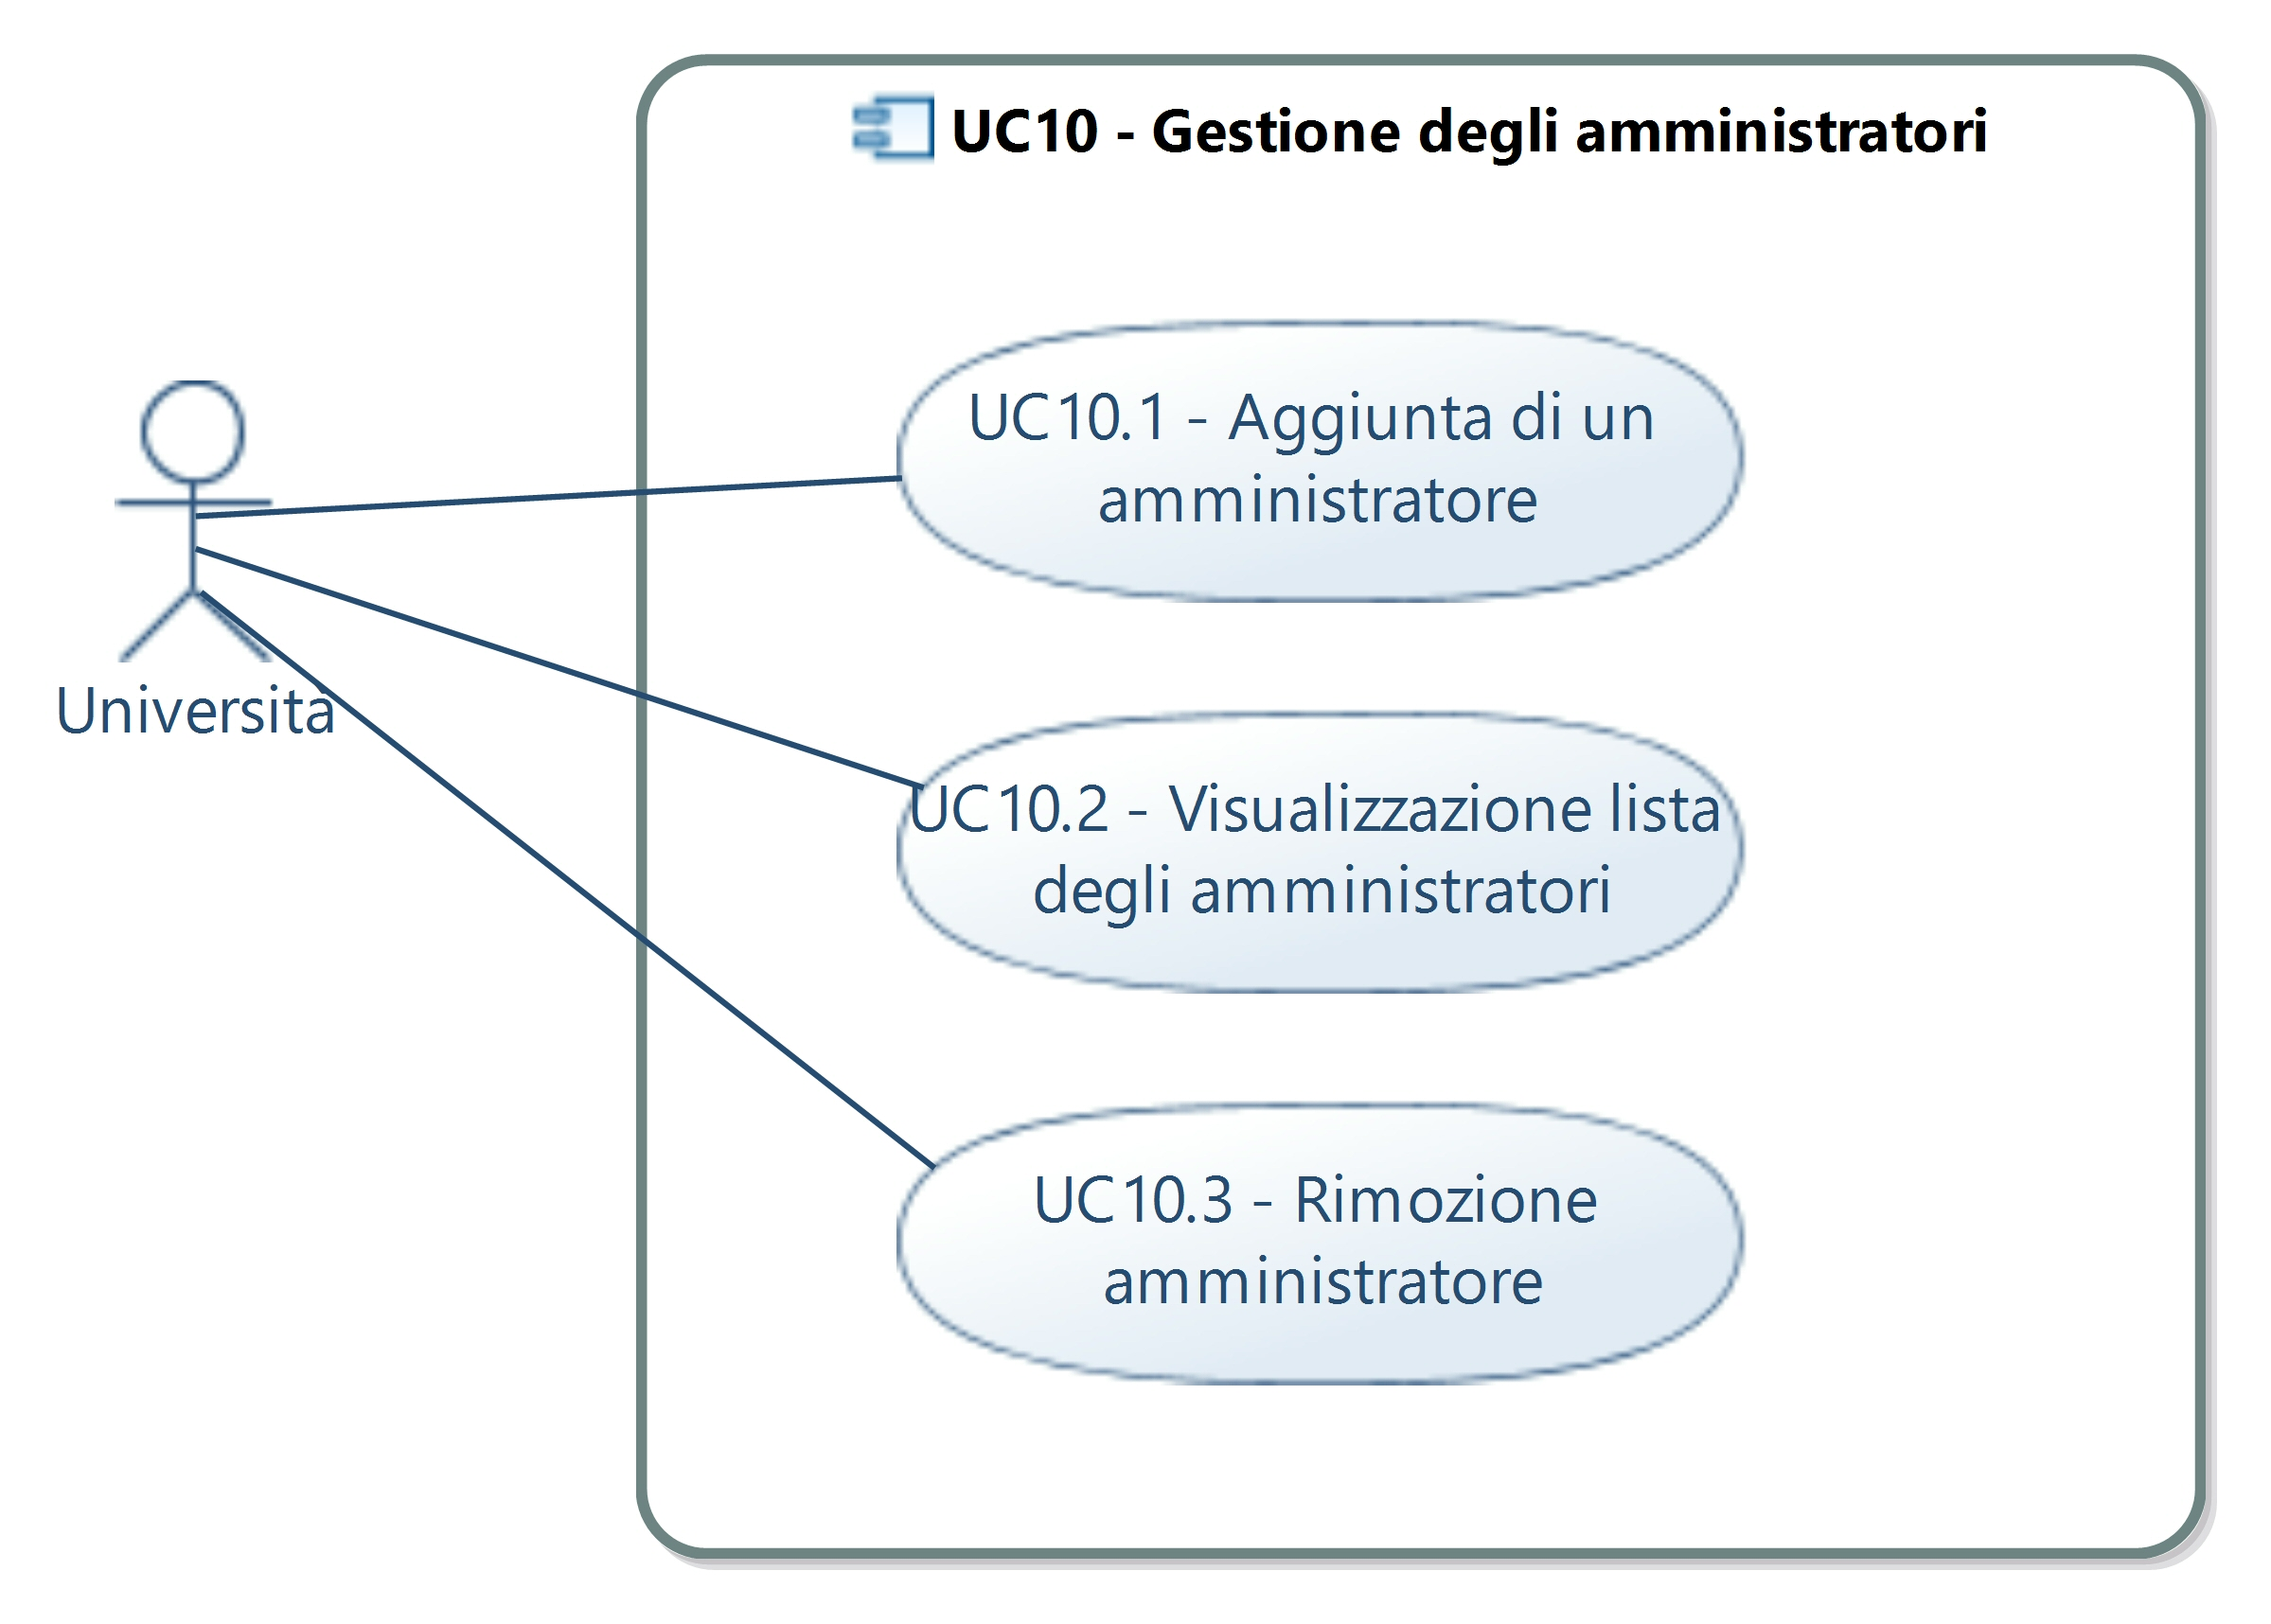
\includegraphics[width=1.0\linewidth]{UC10.jpg}
	\caption{UC10 - Gestione degli amministratori}
	\label{fig:UC10 - Gestione degli amministratori}
\end{figure}

\subsection{UC10.1 - Aggiunta di un amministratore}
\begin{itemize}
	\item \textbf{Attori primari:} università;
	\item \textbf{Scopo e descrizione:} l'utente che rappresenta l'università aggiunge un nuovo amministratore nel sistema, abilitandolo a operare come definito dal sistema;
	\item \textbf{Precondizione:} il sistema riconosce l'utente nel ruolo di rappresentante dell'università e mette a disposizione una serie di operazioni atte alla gestione degli amministratori; 
	\item \textbf{Postcondizione:} all'interno del sistema è stato aggiunto un nuovo amministratore.
\end{itemize}

\begin{figure}[H]
	\centering
	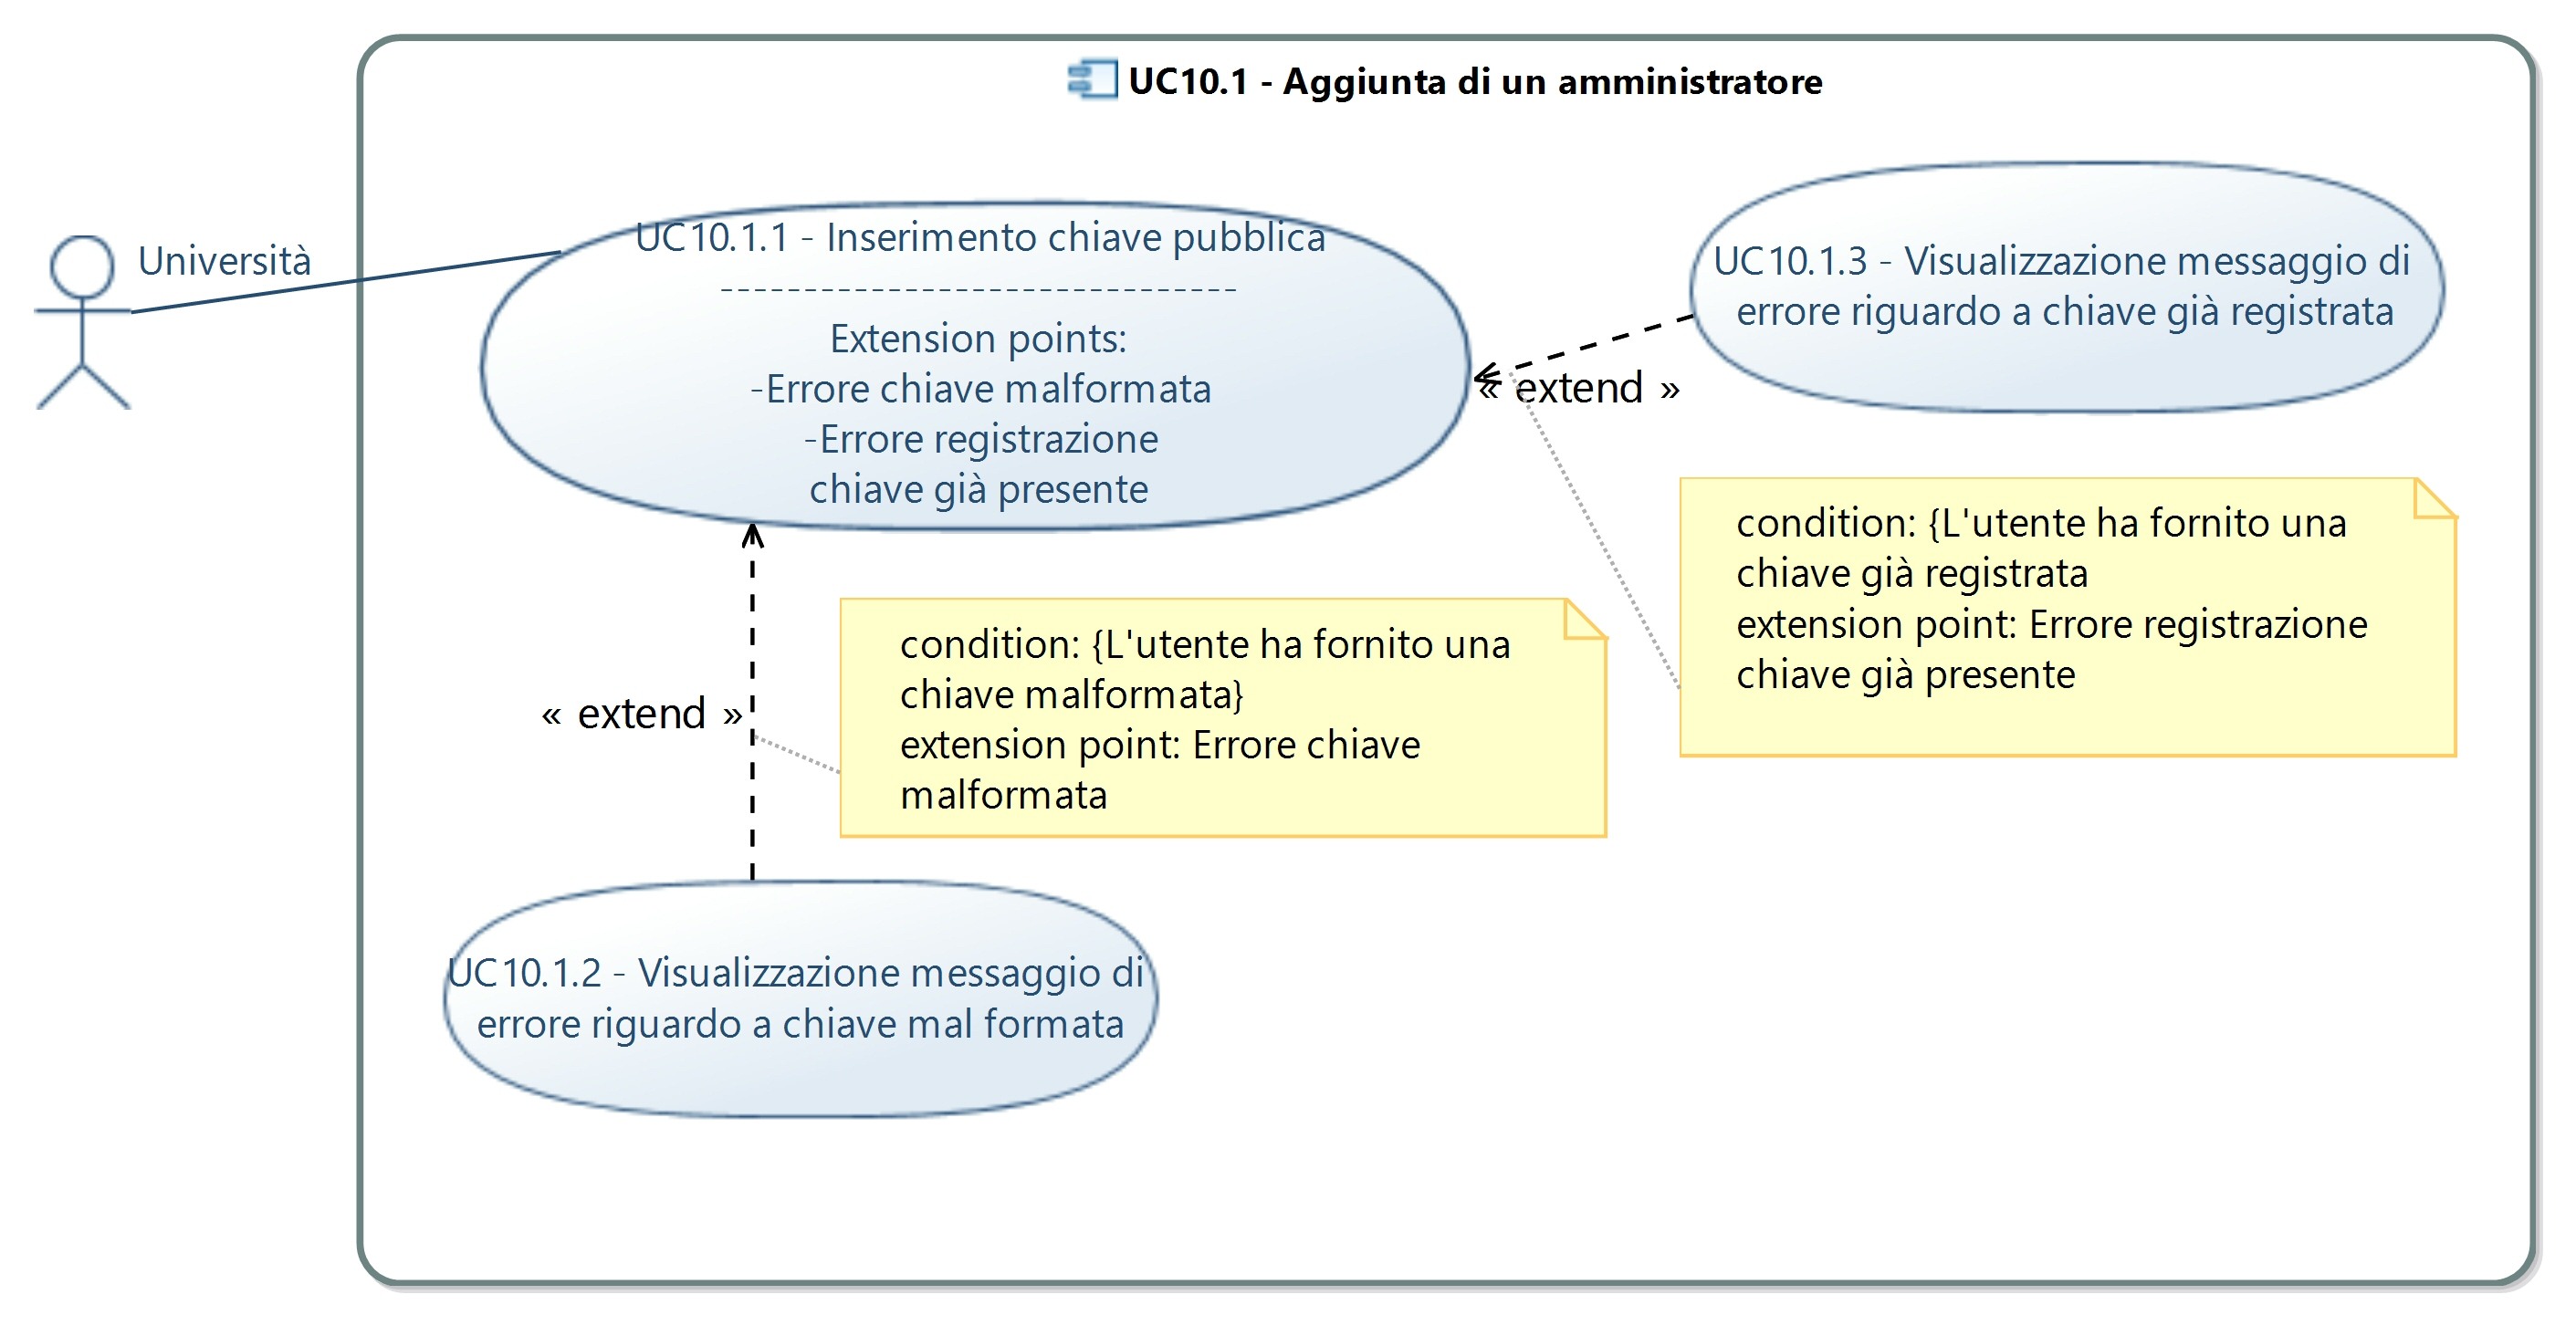
\includegraphics[width=1.0\linewidth]{UC10_1.jpg}
	\caption{UC10.1 - Aggiunta di un amministratore}
	\label{fig:UC10.1 - Aggiunta di un amministratore}
\end{figure}

\subsection{UC10.1.1 - Inserimento chiave pubblica}
\begin{itemize}
	\item \textbf{Attori primari:} università;
	\item \textbf{Scopo e Descrizione:} il sistema offre l'interfaccia per inserire la \citGloss{chiave pubblica} del nuovo amministratore;
	\item \textbf{Scenario principale:} l'utente che rappresenta l'università fornisce tramite un dispositivo di input il suo nome;	\begin{enumerate}
		\item Se la \citGloss{chiave pubblica} è mal formata l'utente viene avvisato con un relativo messaggio d'errore [UC10.1.2];
		\item Se la \citGloss{chiave pubblica} è già registrata nel sistema in un altro ruolo l'utente viene avvisato un relativo messaggio d'errore [UC10.1.3].
	\end{enumerate}
	\item \textbf{Precondizione:} il sistema offre un campo per la compilazione della \citGloss{chiave pubblica} del nuovo amministratore e rimane in attesa dell'input;
	\item \textbf{Postcondizione:} il sistema riceve la \citGloss{chiave pubblica} del nuovo amministratore attraverso il campo precedentemente fornito all'utente.
\end{itemize}
\subsection{UC10.1.2 - Visualizzazione messaggio di errore riguardo a chiave mal formata}
\begin{itemize}
	\item \textbf{Attori primari:} università;
	\item \textbf{Scopo e descrizione:} l'utente viene avvisato del fatto che ha fornito una \citGloss{chiave} mal formata, ad esempio di lunghezza invalida oppure non in caratteri esadecimali;
	\item \textbf{Scenario principale:} l'utente viene informato che la sua \citGloss{chiave} risulta mal formata, invitandolo a ricontrollarla;
	\item \textbf{Precondizione:} il sistema riceve la richiesta di registrazione di una \citGloss{chiave} mal formata;
	\item \textbf{Postcondizione:} il sistema avvisa l'utente di aver richiesto la registrazione di una \citGloss{chiave} mal formata.
\end{itemize}
\subsection{UC10.1.3 - Visualizzazione messaggio di errore riguardo a chiave già registrata}
\begin{itemize}
	\item \textbf{Attori primari:} università;
	\item \textbf{Scopo e descrizione:} l'utente viene avvisato del fatto che ha fornito una \citGloss{chiave} già registrata in un altro ruolo all'interno dell'università, in quanto il suo \citGloss{indirizzo} collide con un secondo precedentemente inserito;
	\item \textbf{Scenario principale:} l'utente viene informato che la sua \citGloss{chiave} risulta già registrata;
	\item \textbf{Precondizione:} il sistema riceve la richiesta di registrazione di una \citGloss{chiave} precedentemente registrata;
	\item \textbf{Postcondizione:} il sistema avvisa l'utente di aver richiesto la registrazione di una \citGloss{chiave} precedentemente registrata.
\end{itemize}


\subsection{UC10.2 - Visualizzazione lista degli amministratori}
\begin{itemize}
	\item \textbf{Attori primari:} università;
	\item \textbf{Scopo e descrizione:} l'utente che rappresenta l'università visualizza una lista di tutti gli amministratori;
	\item \textbf{Scenario principale:} l'utente che rappresenta l'università richiede al sistema la lista degli amministratori per poterla consultare ed eventualmente compiere altre operazioni su di essi;
	\item \textbf{Precondizione:} il sistema riconosce l'utente nel ruolo di rappresentante dell'università e mette a disposizione una serie di operazioni atte alla gestione degli amministratori; 
	\item \textbf{Postcondizione:} il sistema fornisce la lista di tutti gli amministratori presenti.
\end{itemize}

\begin{figure}[H]
	\centering
	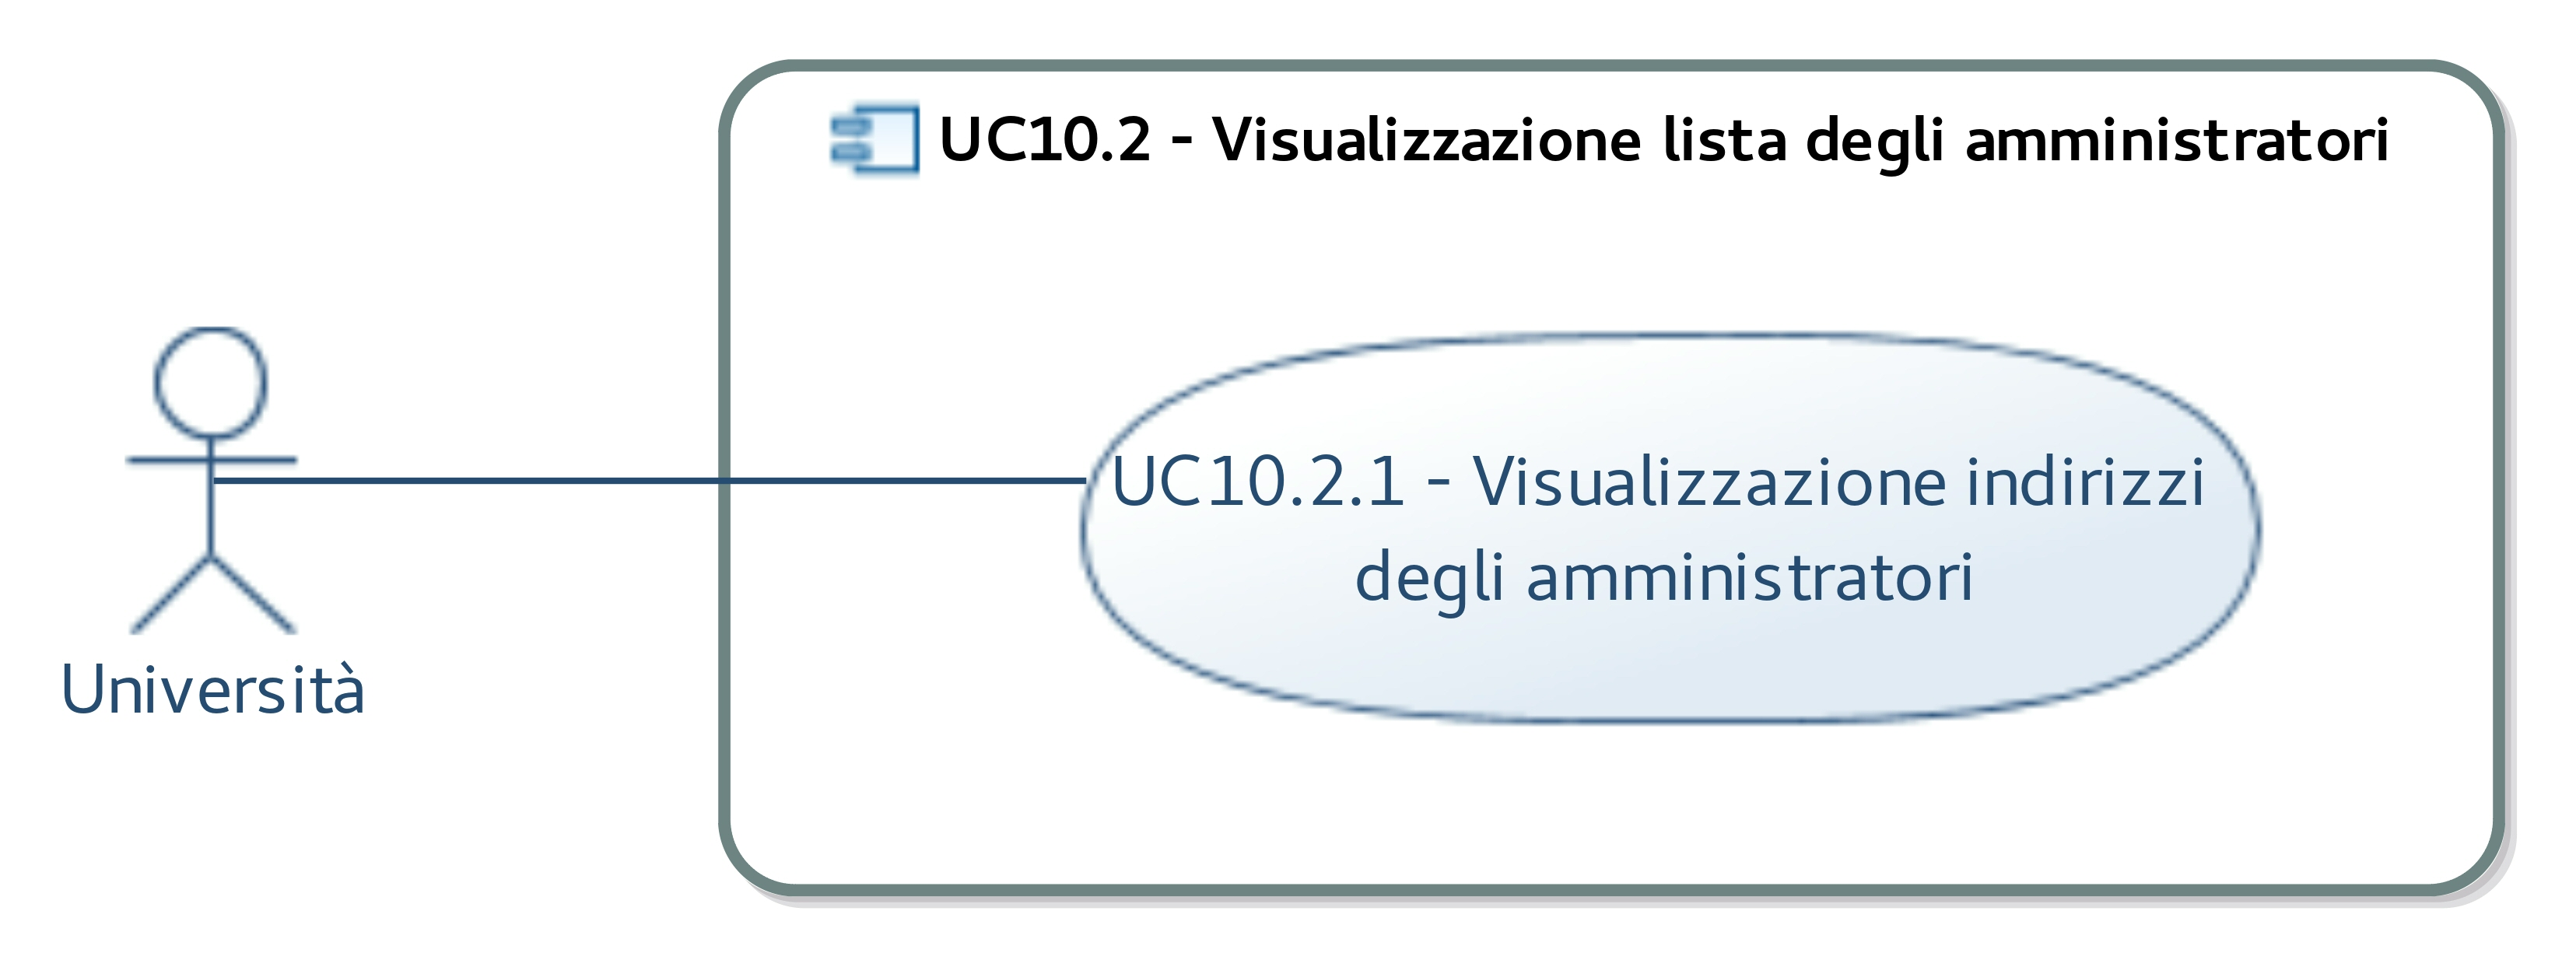
\includegraphics[width=0.7\linewidth]{UC10_2.jpg}
	\caption{UC10.2 - Visualizzazione lista degli amministratori}
	\label{UC10.2 - Visualizzazione lista degli amministratori}
\end{figure}
\subsection{UC10.2.1 - Visualizzazione indirizzi degli amministratori}
\begin{itemize}
	\item \textbf{Attori primari:} università;
	\item \textbf{Scopo e descrizione:} l'utente che rappresenta l'università visualizza per ogni amministratore il suo indirizzo;
	\item \textbf{Scenario principale:} l'utente che rappresenta l'università richiede al sistema la lista dell'indirizzo di ogni amministratore presente;
	\item \textbf{Precondizione:} il sistema riconosce l'utente nel ruolo di rappresentante dell'università, il quale richiede la visualizzazione della lista degli amministratori;
	\item \textbf{Postcondizione:} il sistema fornisce, per ogni amministratore presente, il relativo indirizzo.
\end{itemize}
\subsection{UC10.3 - Rimozione amministratore}
\begin{itemize}
	\item \textbf{Attori primari:} università;
	\item \textbf{Scopo e descrizione:} l'utente che rappresenta l'università rimuove dal sistema un amministratore;
	\item \textbf{Flusso principale degli eventi:}
	\begin{enumerate}
		\item L'utente che rappresenta l'università  visualizza la lista degli amministratori [UC10.2];
		\item L'utente che rappresenta l'università, una volta ottenuta la lista degli amministratori, individua quale desidera rimuovere [UC10.2];
		\item L'utente che rappresenta l'università richiede al sistema l'eliminazione dell'amministratore [UC10.3].
	\end{enumerate}
	\item \textbf{Precondizione:} il sistema riconosce l'utente nel ruolo di rappresentante dell'università e ha precedentemente fornito la lista degli amministratori presenti [UC10.2]; 
	\item \textbf{Postcondizione:} il sistema rimuove l'amministratore indicato.
\end{itemize}

\subsection{UC11 - Visualizzazione quantità di Gas, Ether e costo delle operazioni}
\begin{itemize}
	\item \textbf{Attori primari:} utente generico;
	\item \textbf{Attori secondari:} \citGloss{MetaMask};
	\item \textbf{Scopo e descrizione:} l'utente generico può vedere la quantità di \citGloss{Gas}, \citGloss{Ether} ed euro che andrà a utilizzare per svolgere determinate azioni;
	\item \textbf{Precondizione:} il sistema opera correttamente e riceve una richiesta di visualizzazione della pagina dei costi;
	\item \textbf{Postcondizione:} il sistema fornisce all'utente generico le informazioni da lui richieste e l'utente generico acquisisce l'informazione desiderata.
\end{itemize}

\end{document}
